% ============================================================
% Black-Litterman のビューとリスクのコツ（勉強用）
% コンパイル：tectonic BLMビューとリスクのコツ.tex   （XeTeX 系。2 回目以降は目次と参照がそろう）
% 数値・表・図は ビューとリスクのコツ_計算.py が 生成/ に作る。先にそれを実行すること:
%   （リポジトリの直下で）.venv\Scripts\python.exe 資料集\LLM-BLMビューとリスクのコツ\ビューとリスクのコツ_計算.py
% 本文は 章/ の下のファイルに分けてある。
% ============================================================
\documentclass[xelatex,ja=standard,jafont=haranoaji,a4paper,11pt,openany]{bxjsreport}
\setpagelayout*{left=22mm,right=22mm,top=22mm,bottom=25mm,footskip=11mm}

\usepackage{amsmath,amssymb,mathtools,bm}
\usepackage{booktabs,array,multirow,longtable}
\usepackage{graphicx}
\usepackage{adjustbox}
\usepackage{xcolor}
\usepackage{tikz}
\usetikzlibrary{arrows.meta,positioning,calc,fit}
\usepackage{listings}
\usepackage{enumitem}
\usepackage{caption}
\usepackage[most]{tcolorbox}
\usepackage[hidelinks,bookmarksnumbered]{hyperref}
% しおり（PDF の目次）では数式を使えないので、見出しの記号を文字に置き換える
\pdfstringdefDisableCommands{\def\Omega{Ω}\def\tau{τ}\def\Sigma{Σ}\def\Pi{Π}\def\mu{μ}\def\delta{δ}\def\lambda{λ}%
  \def\propto{∝}\def\CVaR{CVaR}\def\TE{TE}\def\IR{IR}\def\IC{IC}\def\T{ᵀ}}

\graphicspath{{生成/}}

% ---- 色（総合報告書・BLM解説と同じ）
\definecolor{c1}{HTML}{2A78D6}
\definecolor{c2}{HTML}{EB6834}
\definecolor{c3}{HTML}{1BAF7A}
\definecolor{c4}{HTML}{EDA100}
\definecolor{c7}{HTML}{6250D6}
\definecolor{ink2}{HTML}{52514E}
\definecolor{soft1}{HTML}{E4EEF9}
\definecolor{soft2}{HTML}{FBEEDF}
\definecolor{soft3}{HTML}{E3F3E9}
\definecolor{soft4}{HTML}{EEE8FA}
\definecolor{soft5}{HTML}{FDF3DA}

% ---- 計算で作った数値（\V{名前}）
% ビューとリスクのコツ_計算.py が作ったファイル（手で直さない）
\expandafter\def\csname v@idz.lam\endcsname{3.065}
\expandafter\def\csname v@idz.pidiff\endcsname{0.005}
\expandafter\def\csname v@idz.mktvar\endcsname{0.00979}
\expandafter\def\csname v@idz.mktsd\endcsname{9.89}
\expandafter\def\csname v@idz.mktprem\endcsname{3.00}
\expandafter\def\csname v@idz.pSp1\endcsname{2.836}
\expandafter\def\csname v@idz.omhl1\endcsname{0.000709}
\expandafter\def\csname v@idz.ppi1\endcsname{4.80}
\expandafter\def\csname v@idz.pSp2\endcsname{0.563}
\expandafter\def\csname v@idz.omhl2\endcsname{0.000141}
\expandafter\def\csname v@idz.ppi2\endcsname{0.58}
\expandafter\def\csname v@idz.pSp3\endcsname{3.463}
\expandafter\def\csname v@idz.omhl3\endcsname{0.000866}
\expandafter\def\csname v@idz.ppi3\endcsname{2.47}
\expandafter\def\csname v@idz.formdiff\endcsname{\ensuremath{1.7\times 10^{-16}}}
\expandafter\def\csname v@idz.lam1\endcsname{0.0364}
\expandafter\def\csname v@idz.lam2\endcsname{\ensuremath{-}0.1055}
\expandafter\def\csname v@idz.lam3\endcsname{\ensuremath{-}0.0304}
\expandafter\def\csname v@idz.hldiff\endcsname{\ensuremath{3.3\times 10^{-16}}}
\expandafter\def\csname v@idz.erdiff\endcsname{0.005}
\expandafter\def\csname v@idz.wdiff\endcsname{0.01}
\expandafter\def\csname v@idz.wsum\endcsname{103.64}
\expandafter\def\csname v@idz.impl1\endcsname{32.95}
\expandafter\def\csname v@idz.impl2\endcsname{43.06}
\expandafter\def\csname v@idz.impl3\endcsname{33.00}
\expandafter\def\csname v@idz.single\endcsname{50.0, 50.0, 50.0}
\expandafter\def\csname v@idz.omnumdiff\endcsname{0.0000}
\expandafter\def\csname v@idz.omidz1\endcsname{0.002127}
\expandafter\def\csname v@idz.omratio1\endcsname{3.00}
\expandafter\def\csname v@idz.omidz2\endcsname{0.000141}
\expandafter\def\csname v@idz.omratio2\endcsname{1.00}
\expandafter\def\csname v@idz.omidz3\endcsname{0.000466}
\expandafter\def\csname v@idz.omratio3\endcsname{0.54}
\expandafter\def\csname v@idz.ach1\endcsname{16.9}
\expandafter\def\csname v@idz.ach2\endcsname{42.0}
\expandafter\def\csname v@idz.ach3\endcsname{38.2}
\expandafter\def\csname v@idz.omjoint1\endcsname{14.49}
\expandafter\def\csname v@idz.achj1\endcsname{25.8}
\expandafter\def\csname v@idz.omjoint2\endcsname{1.03}
\expandafter\def\csname v@idz.achj2\endcsname{50.1}
\expandafter\def\csname v@idz.omjoint3\endcsname{0.00}
\expandafter\def\csname v@idz.achj3\endcsname{63.2}
\expandafter\def\csname v@idz.joint.res\endcsname{\ensuremath{1.8\times 10^{-2}}}
\expandafter\def\csname v@idz.blsd\endcsname{10.058}
\expandafter\def\csname v@idz.actrisk\endcsname{0.913}
\expandafter\def\csname v@idz.blret\endcsname{3.101}
\expandafter\def\csname v@idz.mktret\endcsname{3.037}
\expandafter\def\csname v@idz.actret\endcsname{0.063}
\expandafter\def\csname v@idz.ir\endcsname{0.069}
\expandafter\def\csname v@meu.pi\endcsname{6.3, 7.1, 7.9, 8.0, 16.5, 9.8}
\expandafter\def\csname v@meu.ppi1\endcsname{7.08}
\expandafter\def\csname v@meu.ppi2\endcsname{6.72}
\expandafter\def\csname v@meu.vsd1\endcsname{24.0}
\expandafter\def\csname v@meu.vsd2\endcsname{33.4}
\expandafter\def\csname v@meu.blspain\endcsname{8.49}
\expandafter\def\csname v@meu.mspain\endcsname{9.54}
\expandafter\def\csname v@meu.full.bl\endcsname{12.00}
\expandafter\def\csname v@meu.full.m\endcsname{12.00}
\expandafter\def\csname v@meu.full.blsd\endcsname{24.0}
\expandafter\def\csname v@meu.full.msd\endcsname{0.00}
\expandafter\def\csname v@meu.unc.blsd\endcsname{28.4}
\expandafter\def\csname v@sim.n\endcsname{400{,}000}
\expandafter\def\csname v@sim.ic\endcsname{0.100}
\expandafter\def\csname v@sim.slope.raw\endcsname{0.0100}
\expandafter\def\csname v@sim.slope.post\endcsname{1.001}
\expandafter\def\csname v@llm.months\endcsname{30}
\expandafter\def\csname v@llm.rows\endcsname{14{,}688}
\expandafter\def\csname v@llm.ic.mean\endcsname{+0.052}
\expandafter\def\csname v@llm.ic.t\endcsname{1.51}
\expandafter\def\csname v@llm.ic.pos\endcsname{14}
\expandafter\def\csname v@llm.icp.mean\endcsname{+0.055}
\expandafter\def\csname v@llm.cin.mean\endcsname{0.89}
\expandafter\def\csname v@llm.slope.mean\endcsname{+0.071}
\expandafter\def\csname v@llm.slope.t\endcsname{1.73}
\expandafter\def\csname v@llm.slope.med\endcsname{+0.067}
\expandafter\def\csname v@llm.slope.pooled\endcsname{+0.074}
\expandafter\def\csname v@llm.ratio.med\endcsname{0.124}
\expandafter\def\csname v@llm.ratio.q25\endcsname{0.042}
\expandafter\def\csname v@llm.ratio.q75\endcsname{0.543}
\expandafter\def\csname v@llm.om.mean\endcsname{\ensuremath{2.89\times 10^{-6}}}
\expandafter\def\csname v@llm.mse\endcsname{\ensuremath{3.65\times 10^{-5}}}
\expandafter\def\csname v@llm.noise\endcsname{\ensuremath{2.04\times 10^{-5}}}
\expandafter\def\csname v@llm.sdQ\endcsname{0.351}
\expandafter\def\csname v@llm.sdr\endcsname{0.411}
\expandafter\def\csname v@llm.omsd\endcsname{0.127}
\expandafter\def\csname v@llm.sd.med\endcsname{1.74}
\expandafter\def\csname v@llm.omtau.med\endcsname{\ensuremath{2.03\times 10^{-1}}}
\expandafter\def\csname v@llm.adopt.med\endcsname{83.09}
\expandafter\def\csname v@blm.tau\endcsname{0.025}
\expandafter\def\csname v@blm.delta\endcsname{2.5}
\expandafter\def\csname v@bt.te.target\endcsname{3}
\expandafter\def\csname v@bt.sample.ann\endcsname{11.5}
\expandafter\def\csname v@bt.sample.effn\endcsname{1.7}
\expandafter\def\csname v@bt.sample.adopt\endcsname{91.3}
\expandafter\def\csname v@bt.sample.te\endcsname{50.9}
\expandafter\def\csname v@bt.sample.ir\endcsname{0.16}
\expandafter\def\csname v@bt.sample.tstat\endcsname{0.25}
\expandafter\def\csname v@bt.hl.ann\endcsname{12.8}
\expandafter\def\csname v@bt.hl.effn\endcsname{1.8}
\expandafter\def\csname v@bt.hl.adopt\endcsname{79.7}
\expandafter\def\csname v@bt.hl.te\endcsname{48.0}
\expandafter\def\csname v@bt.hl.ir\endcsname{0.16}
\expandafter\def\csname v@bt.hl.tstat\endcsname{0.25}
\expandafter\def\csname v@bt.calib.ann\endcsname{\ensuremath{-}0.9}
\expandafter\def\csname v@bt.calib.effn\endcsname{13.5}
\expandafter\def\csname v@bt.calib.adopt\endcsname{43.5}
\expandafter\def\csname v@bt.calib.te\endcsname{43.4}
\expandafter\def\csname v@bt.calib.ir\endcsname{\ensuremath{-}0.16}
\expandafter\def\csname v@bt.calib.tstat\endcsname{\ensuremath{-}0.25}
\expandafter\def\csname v@bt.full.ann\endcsname{25.2}
\expandafter\def\csname v@bt.full.effn\endcsname{17.6}
\expandafter\def\csname v@bt.full.adopt\endcsname{5.6}
\expandafter\def\csname v@bt.full.te\endcsname{26.0}
\expandafter\def\csname v@bt.full.ir\endcsname{0.37}
\expandafter\def\csname v@bt.full.tstat\endcsname{0.58}
\expandafter\def\csname v@bt.fullte.ann\endcsname{17.4}
\expandafter\def\csname v@bt.fullte.effn\endcsname{41.3}
\expandafter\def\csname v@bt.fullte.adopt\endcsname{5.6}
\expandafter\def\csname v@bt.fullte.te\endcsname{5.3}
\expandafter\def\csname v@bt.fullte.ir\endcsname{\ensuremath{-}0.02}
\expandafter\def\csname v@bt.fullte.tstat\endcsname{\ensuremath{-}0.04}
\expandafter\def\csname v@bt.relte.ann\endcsname{17.4}
\expandafter\def\csname v@bt.relte.effn\endcsname{41.3}
\expandafter\def\csname v@bt.relte.adopt\endcsname{1.6}
\expandafter\def\csname v@bt.relte.te\endcsname{5.3}
\expandafter\def\csname v@bt.relte.ir\endcsname{\ensuremath{-}0.02}
\expandafter\def\csname v@bt.relte.tstat\endcsname{\ensuremath{-}0.04}
\expandafter\def\csname v@bt.mkt.ann\endcsname{17.7}
\expandafter\def\csname v@bt.mkt.effn\endcsname{51.5}
\expandafter\def\csname v@bt.mkt.adopt\endcsname{0.0}
\expandafter\def\csname v@bt.b.last\endcsname{0.073}
\expandafter\def\csname v@bt.b.zero\endcsname{6}
\expandafter\def\csname v@bt.months\endcsname{30}
\expandafter\def\csname v@unc.start\endcsname{2015-01}
\expandafter\def\csname v@unc.end\endcsname{2026-09}
\expandafter\def\csname v@unc.epu.med\endcsname{165}
\expandafter\def\csname v@unc.epu.max\endcsname{725}
\expandafter\def\csname v@unc.epu.argmax\endcsname{2025-04}
\expandafter\def\csname v@unc.gpr.med\endcsname{107}
\expandafter\def\csname v@unc.gpr.max\endcsname{330}
\expandafter\def\csname v@unc.gpr.argmax\endcsname{2026-03}
\expandafter\def\csname v@unc.cor.epu\endcsname{0.19}
\expandafter\def\csname v@unc.cor.gpr\endcsname{0.02}
\expandafter\def\csname v@unc.cor.vix\endcsname{0.66}
\expandafter\def\csname v@unc.cor.rv\endcsname{0.55}
\expandafter\def\csname v@unc.reg.n\endcsname{140}
\expandafter\def\csname v@unc.reg.epu.t\endcsname{\ensuremath{-}0.15}
\expandafter\def\csname v@unc.reg.gpr.t\endcsname{\ensuremath{-}0.38}
\expandafter\def\csname v@unc.reg.rv\endcsname{0.56}
\expandafter\def\csname v@unc.reg2.epu.t\endcsname{\ensuremath{-}1.94}
\expandafter\def\csname v@unc.reg2.vix.t\endcsname{5.45}
\expandafter\def\csname v@scen.n\endcsname{99}
\expandafter\def\csname v@scen.dgpr.sd\endcsname{24.4}
\expandafter\def\csname v@scen.depu.sd\endcsname{26.8}
\expandafter\def\csname v@eg.n\endcsname{2{,}952}
\expandafter\def\csname v@eg.ll\endcsname{\ensuremath{-}3{,}738.5}
\expandafter\def\csname v@eg.gamma\endcsname{0.124}
\expandafter\def\csname v@eg.gamma.t\endcsname{0.83}
\expandafter\def\csname v@eg.xi\endcsname{\ensuremath{-}0.157}
\expandafter\def\csname v@eg.beta\endcsname{0.9423}
\expandafter\def\csname v@eg.start\endcsname{2015-01-05}
\expandafter\def\csname v@eg.end\endcsname{2026-09-30}
\expandafter\def\csname v@eg.max\endcsname{103}
\expandafter\def\csname v@eg.argmax\endcsname{2020-03-16}
\expandafter\def\csname v@eg.mu.min\endcsname{\ensuremath{-}0.26}
\expandafter\def\csname v@eg.mu.max\endcsname{15.75}
\expandafter\def\csname v@eg.mu.med\endcsname{0.94}
\expandafter\def\csname v@eg.adopt.min\endcsname{10}
\expandafter\def\csname v@eg.adopt.argmin\endcsname{2020-02}
\expandafter\def\csname v@eg.adopt.max\endcsname{94}
\expandafter\def\csname v@eg.adopt.argmax\endcsname{2020-08}
\expandafter\def\csname v@epu.adopt.min\endcsname{19}
\expandafter\def\csname v@epu.adopt.argmin\endcsname{2025-04}
\expandafter\def\csname v@mom.start\endcsname{1927-05}
\expandafter\def\csname v@mom.end\endcsname{2026-08}
\expandafter\def\csname v@mom.sh.all\endcsname{0.45}
\expandafter\def\csname v@mom.sh.all.sc\endcsname{0.87}
\expandafter\def\csname v@mom.sh.sub\endcsname{0.49}
\expandafter\def\csname v@mom.sh.sub.sc\endcsname{0.94}
\expandafter\def\csname v@mom.dd\endcsname{\ensuremath{-}78}
\expandafter\def\csname v@mom.dd.sc\endcsname{\ensuremath{-}43}
\expandafter\def\csname v@mom.worst.month\endcsname{1932-08}
\expandafter\def\csname v@mom.worst\endcsname{\ensuremath{-}52.6}
\expandafter\def\csname v@mom.2009\endcsname{\ensuremath{-}34.4}
\expandafter\def\csname v@mom.2009.sc\endcsname{\ensuremath{-}10.2}
\expandafter\def\csname v@mom.2009.scale\endcsname{0.30}
\expandafter\def\csname v@sm.months\endcsname{128}
\expandafter\def\csname v@sm.start\endcsname{2016-01}
\expandafter\def\csname v@sm.end\endcsname{2026-08}
\expandafter\def\csname v@sm.cic.mean\endcsname{+0.011}
\expandafter\def\csname v@sm.cic.t\endcsname{0.29}
\expandafter\def\csname v@sm.cic.last\endcsname{0.014}
\expandafter\def\csname v@sm.cic.pos\endcsname{66}
\expandafter\def\csname v@sm.icv.ir\endcsname{\ensuremath{-}0.08}
\expandafter\def\csname v@sm.icv.te\endcsname{3.8}
\expandafter\def\csname v@sm.icv.t\endcsname{\ensuremath{-}0.27}
\expandafter\def\csname v@sm.icv.to\endcsname{15}
\expandafter\def\csname v@sm.icv.ann\endcsname{14.2}
\expandafter\def\csname v@sm.vol.ir\endcsname{\ensuremath{-}0.07}
\expandafter\def\csname v@sm.vol.te\endcsname{3.0}
\expandafter\def\csname v@sm.vol.t\endcsname{\ensuremath{-}0.23}
\expandafter\def\csname v@sm.vol.to\endcsname{13}
\expandafter\def\csname v@sm.vol.ann\endcsname{14.4}
\expandafter\def\csname v@sm.naive.ir\endcsname{0.17}
\expandafter\def\csname v@sm.naive.te\endcsname{15.1}
\expandafter\def\csname v@sm.naive.t\endcsname{0.57}
\expandafter\def\csname v@sm.naive.to\endcsname{34}
\expandafter\def\csname v@sm.naive.ann\endcsname{16.7}
\expandafter\def\csname v@sm.bench.ann\endcsname{14.7}
\expandafter\def\csname v@ep.J\endcsname{20{,}000}
\expandafter\def\csname v@ep.date\endcsname{2026-08-31}
\expandafter\def\csname v@ep.spread0\endcsname{0.50}
\expandafter\def\csname v@ep.tail0\endcsname{1.23}
\expandafter\def\csname v@ep.sdE0\endcsname{6.18}
\expandafter\def\csname v@ep.spread1\endcsname{1.00}
\expandafter\def\csname v@ep.tail1\endcsname{3.00}
\expandafter\def\csname v@ep.sdE1\endcsname{8.04}
\expandafter\def\csname v@ep.ens\endcsname{98.0}
\expandafter\def\csname v@ep.kl\endcsname{0.020}
\expandafter\def\csname v@ep.c.spread\endcsname{0.75}
\expandafter\def\csname v@ep.c.tail\endcsname{2.11}
\expandafter\def\csname v@ep.maxdiff\endcsname{0.001}
\expandafter\def\csname v@cop.c\endcsname{0.5}
\expandafter\def\csname v@cop.loc\endcsname{2}
\expandafter\def\csname v@cop.scale\endcsname{2}
\expandafter\def\csname v@cop.m0\endcsname{0.50}
\expandafter\def\csname v@cop.m1\endcsname{1.25}
\expandafter\def\csname v@cop.sd0\endcsname{8.75}
\expandafter\def\csname v@cop.sd1\endcsname{6.53}
\expandafter\def\csname v@cop.sk0\endcsname{\ensuremath{-}0.01}
\expandafter\def\csname v@cop.sk1\endcsname{\ensuremath{-}0.28}
\expandafter\def\csname v@cop.q05\endcsname{\ensuremath{-}9.6}
\expandafter\def\csname v@cop.q95\endcsname{10.8}
\expandafter\def\csname v@cop.q05.0\endcsname{\ensuremath{-}13.0}
\expandafter\def\csname v@cop.q95.0\endcsname{13.9}
\expandafter\def\csname v@cop.otherdiff\endcsname{0.0000}
\expandafter\def\csname v@cv.target\endcsname{0.41}
\expandafter\def\csname v@cv.mv.cvar\endcsname{7.79}
\expandafter\def\csname v@cv.cv.cvar\endcsname{7.67}
\expandafter\def\csname v@cv.mv.sd\endcsname{3.62}
\expandafter\def\csname v@cv.cv.sd\endcsname{3.62}
\expandafter\def\csname v@te.ir.hl\endcsname{0.028}
\expandafter\def\csname v@te.tau2\endcsname{0.218}
\expandafter\def\csname v@te.tau.base\endcsname{0.913}
\expandafter\def\csname v@te.ir.c90\endcsname{0.06}
\expandafter\def\csname v@te.ir.c50\endcsname{0.03}
\expandafter\def\csname v@fac.Tlong\endcsname{618}
\expandafter\def\csname v@fac.n\endcsname{139}
\expandafter\def\csname v@fac.mom.prior\endcsname{8.2}
\expandafter\def\csname v@fac.adopt120\endcsname{9.1}
\expandafter\def\csname v@fac.share\endcsname{69}
\expandafter\def\csname v@fu.pw.indep\endcsname{0.1616}
\expandafter\def\csname v@fu.best\endcsname{0.5125}
\expandafter\def\csname v@esg.w1diff\endcsname{0.000000}
\expandafter\def\csname v@stk.sig\endcsname{8}
\expandafter\def\csname v@stk.rho\endcsname{0.3}
\expandafter\def\csname v@stk.ic\endcsname{0.05}
\expandafter\def\csname v@stk.check\endcsname{0}
\expandafter\def\csname v@stk.k500.diag\endcsname{27.4}
\expandafter\def\csname v@stk.k500.true\endcsname{0.25}
\expandafter\def\csname v@stk.single\endcsname{0.25}
\expandafter\def\csname v@stk.rhoe\endcsname{0.21}
\expandafter\def\csname v@stk.common.share\endcsname{17}
\expandafter\def\csname v@stk.qlevel.sd\endcsname{0.132}
\expandafter\def\csname v@stk.rlevel.sd\endcsname{0.160}
\expandafter\def\csname v@stk.level.corr\endcsname{\ensuremath{-}0.43}
\expandafter\def\csname v@two.pi1\endcsname{7.50}
\expandafter\def\csname v@two.pi2\endcsname{4.50}
\expandafter\def\csname v@two.q\endcsname{9.50}
\expandafter\def\csname v@two.mu1\endcsname{8.50}
\expandafter\def\csname v@two.mu2\endcsname{4.88}
\expandafter\def\csname v@two.w1\endcsname{70.0}
\expandafter\def\csname v@two.w2\endcsname{40.0}
\expandafter\def\csname v@two.shift2\endcsname{0.38}
\expandafter\def\csname v@two.beta21\endcsname{0.375}
\expandafter\def\csname v@tic.momentum_12m.mean\endcsname{\ensuremath{-}0.005}
\expandafter\def\csname v@tic.momentum_12m.t\endcsname{\ensuremath{-}0.26}
\expandafter\def\csname v@tic.return_1m.mean\endcsname{\ensuremath{-}0.005}
\expandafter\def\csname v@tic.return_1m.t\endcsname{\ensuremath{-}0.31}
\expandafter\def\csname v@tic.relative_momentum_12m.mean\endcsname{0.000}
\expandafter\def\csname v@tic.relative_momentum_12m.t\endcsname{\ensuremath{-}0.02}
\expandafter\def\csname v@tic.volatility_30d.mean\endcsname{+0.002}
\expandafter\def\csname v@tic.volatility_30d.t\endcsname{0.13}
\expandafter\def\csname v@tic.beta_1y.mean\endcsname{+0.024}
\expandafter\def\csname v@tic.beta_1y.t\endcsname{0.98}
\expandafter\def\csname v@tic.pe_trailing.mean\endcsname{+0.006}
\expandafter\def\csname v@tic.pe_trailing.t\endcsname{0.37}
\expandafter\def\csname v@tic.pb.mean\endcsname{\ensuremath{-}0.006}
\expandafter\def\csname v@tic.pb.t\endcsname{\ensuremath{-}0.38}
\expandafter\def\csname v@tic.roe.mean\endcsname{+0.008}
\expandafter\def\csname v@tic.roe.t\endcsname{0.73}
\expandafter\def\csname v@tic.net_margin.mean\endcsname{+0.013}
\expandafter\def\csname v@tic.net_margin.t\endcsname{1.14}
\expandafter\def\csname v@tic.revenue_growth_yoy.mean\endcsname{+0.011}
\expandafter\def\csname v@tic.revenue_growth_yoy.t\endcsname{0.95}
\expandafter\def\csname v@tic.debt_to_equity.mean\endcsname{+0.009}
\expandafter\def\csname v@tic.debt_to_equity.t\endcsname{1.11}
\expandafter\def\csname v@tic.start\endcsname{2015-02}
\expandafter\def\csname v@tic.end\endcsname{2026-08}

\newcommand{\V}[1]{\ifcsname v@#1\endcsname\csname v@#1\endcsname\else\textbf{??#1??}\fi}
\newcommand{\tabin}[1]{\adjustbox{max width=\linewidth}{\input{生成/tab_#1.tex}}}

% ---- よく使う表記
\newcommand{\code}[1]{\texttt{#1}}
\newcommand{\SP}{S\&P500}
\newcommand{\T}{^{\top}}
\newcommand{\muBL}{\mu_{\mathrm{BL}}}
\newcommand{\wmkt}{w_{\mathrm{mkt}}}
\newcommand{\one}{\mathbf{1}}
\newcommand{\E}{\mathrm{E}}
\newcommand{\Var}{\mathrm{Var}}
\newcommand{\Cov}{\mathrm{Cov}}
\newcommand{\IC}{\mathrm{IC}}
\newcommand{\IR}{\mathrm{IR}}
\newcommand{\TE}{\mathrm{TE}}
\newcommand{\CVaR}{\mathrm{CVaR}}
\newcommand{\VaR}{\mathrm{VaR}}
\DeclareMathOperator{\diag}{diag}
\DeclareMathOperator{\tr}{tr}
\newcommand{\figref}[1]{図~\ref{#1}}
\newcommand{\tabref}[1]{表~\ref{#1}}
\newcommand{\chapref}[1]{第~\ref{#1}~章}
\newcommand{\secref}[1]{\ref{#1}~節}
\newcommand{\appref}[1]{付録~\ref{#1}}

\setlist[itemize]{leftmargin=1.6em,itemsep=0.2em,topsep=0.4em}
\setlist[enumerate]{leftmargin=1.8em,itemsep=0.2em,topsep=0.4em}
\captionsetup{font=small,labelfont=bf,skip=6pt}
\renewcommand{\arraystretch}{1.2}

% ---- 図表の置き方（余白を減らす）
\renewcommand{\topfraction}{0.85}
\renewcommand{\bottomfraction}{0.7}
\renewcommand{\textfraction}{0.1}
\renewcommand{\floatpagefraction}{0.75}
\setcounter{totalnumber}{4}

% ---- 章の見出しを小さくする
\makeatletter
\def\@makechapterhead#1{\vspace*{0.3\Cvs}{\parindent\z@\raggedright\normalfont
  \ifnum\c@secnumdepth>\m@ne\if@mainmatter{\Large\headfont\@chapapp\thechapter\@chappos}\par\nobreak\vskip0.4\Cvs\fi\fi
  \interlinepenalty\@M\LARGE\headfont #1\par\nobreak\vskip 1.5\Cvs}}
\def\@makeschapterhead#1{\vspace*{0.3\Cvs}{\parindent\z@\raggedright\normalfont
  \interlinepenalty\@M\LARGE\headfont #1\par\nobreak\vskip 1.5\Cvs}}
\makeatother

% ---- コード
\renewcommand{\lstlistingname}{リスト}
\lstset{basicstyle=\ttfamily\footnotesize,breaklines=true,columns=fullflexible,keepspaces=true,
  showstringspaces=false,frame=single,framerule=0.3pt,rulecolor=\color{black!25},backgroundcolor=\color{black!3},
  xleftmargin=3pt,xrightmargin=3pt,aboveskip=8pt,belowskip=8pt,captionpos=t,
  commentstyle=\color{ink2},keywordstyle=\color{c1},stringstyle=\color{c2!80!black}}

% ---- 囲み
\newtcolorbox{keybox}[1][要点]{enhanced,breakable,colback=soft1,colframe=c1,boxrule=0.5pt,arc=2pt,
  left=8pt,right=8pt,top=6pt,bottom=6pt,title={#1},fonttitle=\sffamily\bfseries\small,coltitle=white}
\newtcolorbox{notebox}[1][注意]{enhanced,breakable,colback=soft2,colframe=c2,boxrule=0.5pt,arc=2pt,
  left=8pt,right=8pt,top=6pt,bottom=6pt,title={#1},fonttitle=\sffamily\bfseries\small,coltitle=white}
\newtcolorbox{exbox}[1][計算例]{enhanced,breakable,colback=soft3,colframe=c3,boxrule=0.5pt,arc=2pt,
  left=8pt,right=8pt,top=6pt,bottom=6pt,title={#1},fonttitle=\sffamily\bfseries\small,coltitle=white}
\newtcolorbox{thmbox}[1][結果]{enhanced,breakable,colback=soft4,colframe=c7,boxrule=0.5pt,arc=2pt,
  left=8pt,right=8pt,top=6pt,bottom=6pt,title={#1},fonttitle=\sffamily\bfseries\small,coltitle=white}
\newtcolorbox{tipbox}[1][コツ]{enhanced,breakable,colback=soft5,colframe=c4!85!black,boxrule=0.5pt,arc=2pt,
  left=8pt,right=8pt,top=6pt,bottom=6pt,title={#1},fonttitle=\sffamily\bfseries\small,coltitle=white}
\newtcolorbox{paperbox}[1][論文]{enhanced,breakable,colback=white,colframe=ink2,boxrule=0.4pt,arc=2pt,
  left=8pt,right=8pt,top=6pt,bottom=6pt,title={#1},fonttitle=\sffamily\bfseries\small,coltitle=white}

% ---- 図の部品
\tikzset{
  box/.style={draw=#1,fill=#1!8,rounded corners=2pt,align=center,font=\footnotesize,inner sep=4pt,
              minimum height=11mm,text width=27mm},
  arr/.style={-{Stealth[length=2mm]},color=ink2,line width=0.6pt},
  lab/.style={font=\scriptsize,color=ink2},
}

\title{Black-Litterman のビューとリスクのコツ\\[6pt]
  \large ビュー $Q$・その不確かさ $\Omega$・$\tau$ の決め方を論文から整理し、\\
  本プロジェクト（LLM-BLM）のデータで確かめる}
\author{勉強用資料}
\date{2026 年 10 月}

\begin{document}
\maketitle
\setcounter{tocdepth}{1}
{\small\tableofcontents}

% ============================================================
\chapter*{この資料について}
\addcontentsline{toc}{chapter}{この資料について}

Black-Litterman モデル（以下 BL）は、市場の時価総額の比率から逆算した「均衡リターン」を出発点にして、投資家の見方（ビュー）を確信の度合いに応じて混ぜ、期待リターンを作り直す方法である。式そのものは短い。難しいのは、式に入れる値を決めることである。とくに次の 3 つは、論文でも実務でも決め方が定まっていない。

\begin{itemize}
\item \textbf{ビューの値 $Q$}：何をどれだけ上がる（下がる）と見るか。
\item \textbf{ビューの不確かさ $\Omega$}：そのビューをどれだけ信じるか。
\item \textbf{均衡の不確かさの大きさ $\tau$}：出発点の均衡リターンをどれだけ信じるか。
\end{itemize}

この資料は、この 3 つ（と、それに関わる共分散 $\Sigma$、ビューの形 $P$）の決め方の「コツ」を、論文を読んで整理し、本プロジェクト（LLM-BLM）のデータで実際に計算して確かめるものである。

\section*{ほかの資料との関係}

\begin{center}
\small
\begin{tabular}{p{3.0cm}p{10.6cm}}
\toprule
資料 & 内容 \\
\midrule
『BLM解説』（勉強用） & 平均分散最適化から BL までの基礎。He と Litterman（1999）に沿って、公式の導き方と G7 の例を手で計算する \\
『総合報告書』 & 対象論文（arXiv 2504.14345）の再現と検証、データ基盤、実験 A〜G。元の計算の問題点（ビューが 99.9\% 採用される、回答のばらつきは信頼度ではない、など） \\
この資料 & ビュー・不確かさ・$\tau$ の決め方。論文ごとの方法の整理と、その数値例。本プロジェクトの LLM の回答で $\Omega$ の決め方を比べ直す \\
\bottomrule
\end{tabular}
\end{center}

基礎は『BLM解説』と重なるところもあるが、この資料だけで読めるように、必要な式は導き直している。

\section*{依頼のときに渡された調査メモについて}

この資料は、依頼のときに渡された文章（以下「調査メモ」）を骨組みにしている。調査メモは、BL のビューとリスクを数値化する方法を、政治・マクロ経済・財務（ESG を含む）・モメンタムの 4 つのファクターに分けて整理し、ファクター版の BL、エントロピー・プーリング、トラッキングエラー付きの最適化にも触れている。

調査メモには、確かめられる主張と、確かめられない主張が混ざっている。この資料では、論文の本文または要旨で確認できたことだけを事実として書いた。確認できなかったもの、論文と食い違うものは、\appref{app:check} に一覧にした。主なものを挙げる。

\begin{itemize}
\item Sun ほか（2026）の「年率 106.58\%、シャープレシオ 2.64」は論文の数字どおりである。ただし、対象は 8 銘柄、評価期間は 117 取引日で、ビューの不確かさは単位行列と書かれている（\chapref{ch:text}）。
\item 対象論文が回答を 100 回取るのは第 2 版である。第 1 版と本プロジェクトは 30 回である。
\item 「ESG の点数で共分散を $(2-\mathrm{ESG})$ 倍に膨らませる」方法と、「景気循環のビューと CVaR を組み合わせてシャープレシオが平均 19.7\% 改善した」という研究は、出典を見つけられなかった（\chapref{ch:esg}、\chapref{ch:macro}）。
\item 「LLM の回答のばらつきが、情報の不確かさを客観的に表す」という主張は、本プロジェクトのデータでは成り立たない。回答の分散は、実際の予想の誤差の 2 乗の中央値で \V{llm.ratio.med} 倍しかない（\chapref{ch:project}）。
\end{itemize}

\section*{構成}

\begin{center}
\small
\begin{tabular}{p{2.4cm}p{11.2cm}}
\toprule
部 & 内容 \\
\midrule
第 I 部 基礎 & BL の全体像。公式の 3 通りの導き方。均衡リターンとリスク回避度。$\tau$ の意味と決め方 \\
第 II 部 $\Omega$ の決め方 & 方法の一覧。Idzorek の確信度の方法を例で再現する。He--Litterman と Meucci の流儀。予想の当たり具合（IC）から決める方法。ビューが多いときの確信の積み上がり。ビューの形（絶対・相対・順位・ファクター） \\
第 III 部 ファクターごとの数値化 & 政治と政策の不確かさ（GPR、EPU）。テキストのセンチメントと LLM。マクロとボラティリティ（EGARCH-M）。財務と ESG。モメンタム \\
第 IV 部 拡張と最適化 & エントロピー・プーリング。コピュラ・オピニオン・プーリング。CVaR の最適化。トラッキングエラーと情報レシオ \\
第 V 部 当てはめ & 本プロジェクトの LLM のビューで $\Omega$ の決め方を比べる。コツの一覧。まとめ \\
付録 & 行列の公式。調査メモの主張の確認表。論文の一覧。作り直し方。Python での実装例。用語集。参考文献 \\
\bottomrule
\end{tabular}
\end{center}

急ぐ読者は、\chapref{ch:overview}（全体像）、\chapref{ch:accuracy}（当たり具合から $\Omega$ を決める）、\chapref{ch:project}（本プロジェクトでの比較）、\chapref{ch:tips}（コツの一覧）を読めば要点がつかめる。

\section*{数字の出どころ}

本文の数値・表・図は、すべて \code{ビューとリスクのコツ\_計算.py} が計算して \code{生成/} に書き出したものである。本文に数字を手で書き写していない。使ったデータは次のとおりである（詳しくは \appref{app:rebuild}）。

\begin{itemize}
\item 本プロジェクトの DB（\code{data/blm\_2015.sqlite}）：株価、指数、セクター ETF、\SP{} の構成銘柄と時価総額、LLM の回答（実行番号 1、gpt-4o-mini、30 か月、約 44 万個）。
\item Kenneth French のデータライブラリ：Fama--French の 5 ファクターとモメンタム（月次・日次）。
\item 経済政策不確実性指数（EPU、Baker・Bloom・Davis）と地政学リスク指数（GPR、Caldara・Iacoviello）の月次の値。
\item 論文に載っている数値例（Idzorek の 8 資産、Meucci の 6 か国、対象論文の表）。
\end{itemize}

論文の数値例は、論文の表と照らし合わせて再現できることを確かめてから使った。例えば Idzorek の例では、事後の期待リターンが論文の表と最大 \V{idz.erdiff}\% の差で一致する。

\section*{記号}

\begin{center}
\small
\begin{tabular}{p{2.2cm}p{11.4cm}}
\toprule
記号 & 意味 \\
\midrule
$N$、$K$ & 資産の数、ビューの数 \\
$r$（または $X$） & 資産のリターン（無リスク金利を引いた超過リターン）。$N$ 次元 \\
$\mu$ & 期待リターン（分からない量）。$N$ 次元 \\
$\Sigma$ & リターンの共分散行列（$N\times N$） \\
$\wmkt$ & 時価総額の比率（市場ポートフォリオ） \\
$\delta$（$\lambda$） & リスク回避度。論文によって $\delta$ と $\lambda$ の両方が使われる \\
$\Pi$（$\pi$） & 均衡リターン $\Pi=\delta\Sigma\wmkt$ \\
$\tau$ & 均衡の不確かさの大きさ。事前分布 $\mu\sim\mathcal N(\Pi,\tau\Sigma)$ \\
$P$ & ビューの組み合わせを表す行列（$K\times N$）。$k$ 行目を $p_k$ と書く \\
$Q$（$v$、$q$） & ビューの値（$K$ 次元） \\
$\Omega$ & ビューの不確かさ（$K\times K$、多くは対角）。対角成分を $\omega_k$ と書く \\
$\muBL$、$M$ & 事後の期待リターンと、その不確かさ（事後の共分散） \\
$C_k$ & Idzorek の確信度（0〜100\%） \\
$c$ & Meucci の確信度（$\Omega=\frac{1}{c}P\Sigma P\T$） \\
$s$ & ビューの採用率。均衡からビューへ何割動くか（1 資産なら $s=\tau\sigma^2/(\tau\sigma^2+\omega)$） \\
IC & 予想と実際のリターンの相関（情報係数） \\
TE、IR & トラッキングエラー（ベンチマークからのずれの標準偏差）、情報レシオ（超過リターン ÷ TE） \\
\bottomrule
\end{tabular}
\end{center}

\section*{要約：この資料で確かめたこと}

\begin{keybox}[要約]
\begin{enumerate}
\item BL の結果を決めるのは、$\Omega$ と $\tau\Sigma$ の大きさの比である。1 資産・1 ビューなら、均衡からビューへ動く割合は $s=\tau\sigma^2/(\tau\sigma^2+\omega)$ になる。$\Omega$ を $\tau$ に比例させると、事後の期待リターンから $\tau$ が消える（\chapref{ch:tau}）。
\item Idzorek の確信度の方法は、閉じた式 $\omega_k=\tau p_k\Sigma p_k\T(1-C_k)/C_k$ と同じ結果になる。ただし、指定した確信度どおりに比率が動くのはビューが 1 つのときだけで、3 つ同時に入れた例では、65\% と指定したビューが \V{idz.ach3}\% しか動かなかった（\chapref{ch:idzorek}）。
\item 予想の当たり具合を IC で測れば、$\Omega$ を決められる。Meucci の市場版の BL で $\omega=\sigma^2(1/\IC^2-1)$ と置くと、Grinold の式 $\alpha=\IC\cdot\sigma\cdot z$ と同じになる。IC が 0.05 なら、採用率は 0.25\% である（\chapref{ch:accuracy}）。
\item ビューが多いときは、$\Omega$ を対角にしてはいけない。誤差の相関を無視すると、銘柄の数だけ確信が積み上がる。本プロジェクトのデータでは、1 銘柄あたり数 \% のはずの採用率が、対角の $\Omega$ では中央値 \V{bt.calib.adopt}\% になった（\chapref{ch:project}）。
\item LLM の回答のばらつきは、当たり具合を表さない。回答の分散は、実際の誤差の 2 乗の中央値の \V{llm.ratio.med} 倍で、予想を 8 倍前後信じすぎる設定になる（\chapref{ch:project}）。
\item 政治・政策の指数（EPU、GPR）は、直近のボラティリティや VIX を入れると、翌月のボラティリティを説明する力がほとんど残らなかった。$\Omega$ を伸び縮みさせる材料としては、市場のボラティリティのほうが強い（\chapref{ch:politics}）。
\item モメンタムは、ボラティリティで規模を調整すると、急落が小さくなり、シャープレシオが \V{mom.sh.all} から \V{mom.sh.all.sc} に上がった。ビューの確信度を「モメンタム自身の最近のボラティリティ」で割るのは理にかなう（\chapref{ch:momentum}）。
\item 平均のビューだけなら、エントロピー・プーリングは市場版の BL とほぼ同じ答えを出す（差は最大 \V{ep.maxdiff}\%）。違いが出るのは、順位・ボラティリティ・下落確率のような、平均以外のビューを入れたときである（\chapref{ch:ep}）。
\item 予想が正しく縮められていても、平均分散最適化はトラッキングエラーを大きく取りがちである。トラッキングエラーの上限をはっきり置くほうがよい（\chapref{ch:te}、\chapref{ch:project}）。
\end{enumerate}
\end{keybox}


\part{基礎}
% ============================================================
\chapter{Black-Litterman の全体像：何をどこで決めるか}\label{ch:overview}

この章では、BL の計算の流れをたどり、決めなければならない値を一覧にする。そのうえで、この資料の中心になる「採用率」という見方を、1 資産・1 ビューの場合で導く。

\section{平均分散最適化の弱点と、BL の考え方}

平均分散最適化は、期待リターン $\mu$ と共分散 $\Sigma$ から、リスク回避度 $\delta$ のもとで
\begin{equation}
\max_w\; w\T\mu-\frac{\delta}{2}w\T\Sigma w
\label{eq:mvobj}
\end{equation}
を解く。制約がなければ答えは $w^*=(\delta\Sigma)^{-1}\mu$ である。この式は $\mu$ の小さな違いに非常に敏感で、過去の平均リターンを $\mu$ に入れると、極端な買いと売りが並ぶ比率になる。Idzorek（2007）の 8 資産の例では、過去 60 か月の平均を使うと、米国債券が 1144\%、外国債券が $-105\%$ という比率になる（\chapref{ch:idzorek}）。$\mu$ の推定の誤差が、最適化で増幅されるためである（Michaud 1989 の言う「誤差の最大化」）。

BL は、$\mu$ を直接推定しない。まず、いまの時価総額の比率 $\wmkt$ が式~\eqref{eq:mvobj} の答えになっていると仮定して、$\mu$ を逆算する。
\begin{equation}
\Pi=\delta\Sigma\wmkt
\label{eq:pi}
\end{equation}
これを均衡リターンと呼ぶ。$\Pi$ を最適化に入れれば、答えは $\wmkt$ に戻る。つまり、ビューがなければ市場の比率を持つ。そのうえで、投資家のビューを確信の度合いに応じて混ぜ、$\Pi$ を少しだけ動かす。動かした分だけ、比率が市場からずれる。

\section{計算の流れ}

\begin{figure}[htbp]
\centering
\adjustbox{max width=\linewidth}{%
\begin{tikzpicture}[node distance=6mm and 8mm]
\node[box=c3] (w) {時価総額の比率\\$\wmkt$};
\node[box=c3,right=of w] (pi) {均衡リターン\\$\Pi=\delta\Sigma\wmkt$};
\node[box=c3,above=5mm of pi] (sig) {共分散 $\Sigma$\\リスク回避度 $\delta$};
\node[box=c4,below=12mm of w] (src) {ビューの材料\\（分析・モデル・LLM）};
\node[box=c4,right=of src] (q) {ビュー $P$, $Q$\\不確かさ $\Omega$};
\node[box=c1,right=14mm of $(pi)!0.5!(q)$] (bl) {BL の事後\\$\muBL$、$M$\\（$\tau$ を使う）};
\node[box=c1,right=of bl] (opt) {最適化\\（制約・TE）};
\node[box=c2,right=of opt] (wt) {投資比率\\$w$};
\draw[arr] (w) -- node[lab,above]{逆最適化} (pi);
\draw[arr] (sig) -- (pi);
\draw[arr] (src) -- node[lab,above]{数値化} (q);
\draw[arr] (pi) -- (bl);
\draw[arr] (q) -- (bl);
\draw[arr] (bl) -- (opt);
\draw[arr] (opt) -- (wt);
\draw[arr] (sig.east) -| (opt.north);
\end{tikzpicture}}
\caption{BL の計算の流れ。緑は市場から決まる部分、黄はビューの部分、青は混ぜる部分と最適化。共分散 $\Sigma$ は、均衡リターン、BL、最適化の 3 か所で使う。}
\label{fig:flow}
\end{figure}

\figref{fig:flow} の流れを言葉で書くと、次のようになる。

\begin{enumerate}
\item 共分散 $\Sigma$ を推定し、リスク回避度 $\delta$ を決める。
\item 時価総額の比率から、均衡リターン $\Pi$ を逆算する。
\item ビューを $P\mu=Q+\varepsilon$、$\varepsilon\sim\mathcal N(0,\Omega)$ の形に書く。
\item 均衡の不確かさ $\tau\Sigma$ とビューの不確かさ $\Omega$ の比で、$\Pi$ と $Q$ を混ぜる。結果が事後の期待リターン $\muBL$ である。
\item $\muBL$ と $\Sigma$（または事後の共分散）で最適化する。制約（空売りなし、上限、トラッキングエラー）はここで入れる。
\end{enumerate}

\section{決めるものの一覧}

\begin{table}[htbp]
\centering
\caption{BL で決めるもの。右端は、この資料で扱う章。}
\label{tab:knobs}
\small
\begin{tabular}{p{1.4cm}p{2.9cm}p{6.2cm}p{2.0cm}}
\toprule
記号 & 意味 & よく使われる決め方 & 章 \\
\midrule
$\Sigma$ & リターンの共分散 & 標本共分散、縮小推定（Ledoit--Wolf）、ファクターモデル、GARCH & \ref{ch:prior}、\ref{ch:macro} \\
$\delta$ & リスク回避度 & 市場の超過リターン ÷ 市場の分散。2.5 前後がよく使われる & \ref{ch:prior} \\
$\Pi$ & 均衡リターン & $\delta\Sigma\wmkt$。ベンチマークの比率や、ESG で調整した比率を使う例もある & \ref{ch:prior}、\ref{ch:esg} \\
$\tau$ & 均衡の不確かさ & 0.01〜0.05、$1/T$、1。$\Omega$ を $\tau$ に比例させると消える & \ref{ch:tau} \\
$P$ & ビューの形 & 絶対（1 資産）、相対（差）、順位、ファクター & \ref{ch:shape} \\
$Q$ & ビューの値 & 分析者の見方、統計モデルの予想、IC で縮めた値 & \ref{ch:accuracy}〜\ref{ch:momentum} \\
$\Omega$ & ビューの不確かさ & $\tau P\Sigma P\T$、確信度から逆算（Idzorek）、予想の誤差の分散、モデルの条件付き分散、回答のばらつき & \ref{ch:omega}〜\ref{ch:accuracy} \\
最適化 & 比率の決め方 & 制約なし、空売りなし、上限、トラッキングエラー、CVaR & \ref{ch:cvar}、\ref{ch:te} \\
\bottomrule
\end{tabular}
\end{table}

\tabref{tab:knobs} のうち、$\Sigma$ と $\delta$ は市場のデータから比較的はっきり決まる。決め方に幅があり、結果を大きく左右するのは $\tau$、$Q$、$\Omega$ である。この資料の大半は、この 3 つの話である。

\section{1 資産・1 ビューで見る「採用率」}\label{sec:adoption}

BL の公式（\chapref{ch:derive} で導く）は、1 資産・1 ビューの場合に次の形になる。資産のリターンの分散を $\sigma^2$、均衡リターンを $\pi$、ビューの値を $q$、その不確かさを $\omega$ とする。
\begin{equation}
\mu_{\mathrm{BL}}=\pi+\underbrace{\frac{\tau\sigma^2}{\tau\sigma^2+\omega}}_{s}\,(q-\pi)
\label{eq:scalar}
\end{equation}
$s$ は、均衡 $\pi$ からビュー $q$ へ何割動くかを表す。この資料では $s$ を「採用率」と呼ぶ。採用率は、2 つの不確かさの比 $\omega/(\tau\sigma^2)$ だけで決まる。
\begin{equation}
s=\frac{1}{1+\omega/(\tau\sigma^2)}
\label{eq:adoption}
\end{equation}

\begin{figure}[htbp]
\centering
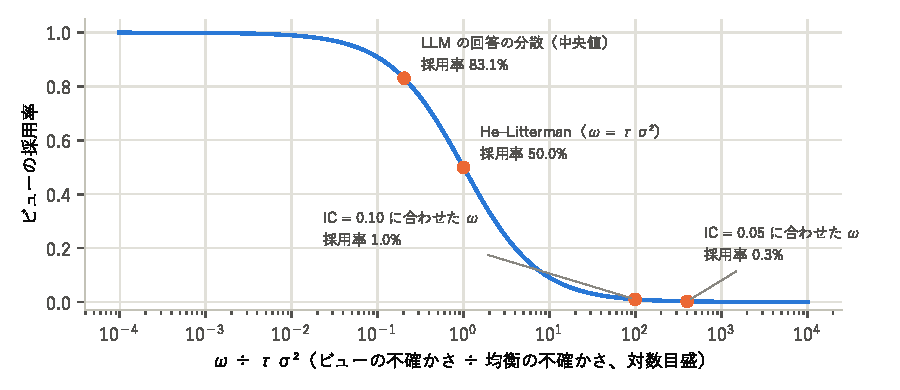
\includegraphics[width=0.92\linewidth]{fig_adoption_curve.pdf}
\caption{採用率と、2 つの不確かさの比の関係（式~\eqref{eq:adoption}）。点は、この資料で扱う設定。LLM の回答の分散は本プロジェクトのデータ（$\tau=0.025$、過去 1 年の日次の分散 $\sigma^2$ との比の中央値）。IC に合わせた $\omega$ は \chapref{ch:accuracy} の式~\eqref{eq:omega-ic} による。}
\label{fig:adoption}
\end{figure}

\figref{fig:adoption} から分かることを挙げる。

\begin{itemize}
\item He と Litterman の設定 $\omega=\tau\sigma^2$ では、採用率はちょうど 50\% である。ビューと均衡を同じ重みで扱う。
\item 本プロジェクトの LLM の回答の分散を $\omega$ に使うと、1 銘柄だけで見ても採用率は \V{llm.adopt.med}\% になる。複数の銘柄を同時に入れると、さらに高くなる（\chapref{ch:project}）。
\item 予想の当たり具合（IC）に合わせると、採用率は IC の 2 乗になる。IC が 0.05 なら 0.25\%、0.10 でも 1\% である。予想の当たり具合が現実的な水準なら、ビューはほとんど採用されないのが正しい。
\end{itemize}

採用率が 50\% と 1\% では、比率は大きく違う。$\Omega$ と $\tau$ を「なんとなく」決めると、結果の大半がその選び方で決まってしまう。これが、この資料の出発点である。

\section{大きさの感覚}\label{sec:scale}

$\tau\sigma^2$ と $\omega$ は、どちらも「期待リターンの不確かさ」の分散である。数字にしてみる。

\begin{exbox}[大きさの例（年率）]
株式の年率の標準偏差を $\sigma=20\%$ とすると、$\sigma^2=0.04$ である。$\tau=0.025$ なら $\tau\sigma^2=0.001$、その平方根は 3.2\% である。つまり事前分布は「期待リターンは均衡リターンのまわりに、標準偏差 3.2\% でばらつく」と言っている。

ビューの不確かさを、標準偏差で 3.2\% と置けば採用率は 50\%、10\% と置けば採用率は $0.001/(0.001+0.01)=9\%$、1\% と置けば 91\% である。「1 年後のリターンを ±1\% の精度で知っている」と言える投資家はいないので、91\% は信じすぎである。
\end{exbox}

単位にも注意がいる。日次・月次・年率のどれで書くかによって、$\sigma^2$ も $\omega$ も変わる。比 $\omega/(\tau\sigma^2)$ は、両方を同じ単位で書いていれば単位によらない。本プロジェクトのように「翌月の日次の平均リターン」を予想させる場合、$\Sigma$ は日次のリターンの共分散、$\omega$ も日次の平均リターンの分散でそろえる。元の実装では、日次のリターンから年率の金利を引いていた（『総合報告書』問題 5）。単位のずれは、採用率をそのまま狂わせる。

\section{調査メモの 4 つのファクターとの対応}

調査メモは、ビューと不確かさを作る材料を 4 つのファクターに分けている。この資料での扱いを\tabref{tab:factors}にまとめる。

\begin{table}[htbp]
\centering
\caption{調査メモのファクターと、この資料での扱い。}
\label{tab:factors}
\small
\begin{tabular}{p{1.8cm}p{4.2cm}p{5.0cm}p{1.4cm}}
\toprule
ファクター & ビュー $Q$ の作り方 & 不確かさ $\Omega$ の作り方 & 章 \\
\midrule
政治 & 地政学リスク・政策不確実性への感応度、シナリオ & 指数の水準で $\Omega$ を伸び縮みさせる（Han and Li 2023） & \ref{ch:politics} \\
テキスト・LLM & センチメント、LLM の予想（平均） & 回答のばらつき、確率の分布のエントロピー、複数のモデルの融合 & \ref{ch:text} \\
マクロ & 時系列モデル（EGARCH-M など）の予想 & 条件付き分散（Beach and Orlov 2007） & \ref{ch:macro} \\
財務・ESG & ファクターのプレミアム × 露出 & ファクターのプレミアムの推定誤差。ESG は共分散ではなく平均か制約で & \ref{ch:esg} \\
モメンタム & 過去のリターンの順位 & 予想の当たり具合（IC）、モメンタムのボラティリティ & \ref{ch:momentum} \\
\bottomrule
\end{tabular}
\end{table}

どのファクターでも、考えることは同じである。

\begin{enumerate}
\item ビューの値 $Q$ を、予想の当たり具合に見合った大きさにする（\chapref{ch:accuracy}）。
\item 不確かさ $\Omega$ を、実際の予想の誤差の大きさに合わせる。誤差の相関も入れる（\chapref{ch:accuracy}、\chapref{ch:project}）。
\item 最適化の段階で、ずれの大きさ（トラッキングエラー）に上限を置く（\chapref{ch:te}）。
\end{enumerate}

\begin{keybox}[この章のまとめ]
\begin{itemize}
\item BL で結果を大きく左右するのは $\tau$、$Q$、$\Omega$ の 3 つである。
\item 1 資産・1 ビューなら、均衡からビューへ動く割合（採用率）は $\tau\sigma^2/(\tau\sigma^2+\omega)$ である。
\item He--Litterman の設定では採用率は 50\%、予想の当たり具合に合わせると IC の 2 乗（多くは 1\% 未満）になる。この差が、BL の結果の差の大部分を生む。
\end{itemize}
\end{keybox}

% ============================================================
\chapter{公式の 3 通りの導き方}\label{ch:derive}

BL の公式は、少なくとも 3 通りに導ける。混合推定（一般化最小二乗）、ベイズの定理、罰則つきの最小二乗である。どれも同じ答えになるが、見え方が違う。$\Omega$ や $\tau$ の意味を考えるとき、どの見方で考えているかを意識すると混乱が減る。

\section{設定：2 段の確率モデル}

真の期待リターン $\mu$（$N$ 次元）は分からないので、確率変数として扱う。BL は 2 つの情報源を持つ。

\begin{description}[leftmargin=2em,style=nextline]
\item[均衡（事前の情報）] $\mu$ は均衡リターン $\Pi$ のまわりに散らばる。
\begin{equation}
\mu=\Pi+\eta,\qquad \eta\sim\mathcal N(0,\tau\Sigma)
\label{eq:prior}
\end{equation}
\item[ビュー（追加の情報）] $\mu$ のいくつかの組み合わせについて、値の見込みがある。
\begin{equation}
P\mu=Q+\varepsilon,\qquad \varepsilon\sim\mathcal N(0,\Omega)
\label{eq:view}
\end{equation}
\end{description}

$P$ は $K\times N$ の行列で、$k$ 行目 $p_k$ が $k$ 番目のビューの組み合わせを表す。$\eta$ と $\varepsilon$ は独立とする。$\Omega$ は多くの場合対角で、ビューどうしの誤差は独立と仮定される。この仮定は、ビューが多いときに大きな問題になる（\chapref{ch:accuracy}、\chapref{ch:project}）。

ここで扱っているのは $\mu$、つまり「期待リターン」である。実現するリターン $r$ そのものではない。$r$ は $\mu$ のまわりに $\Sigma$ で散らばる。
\begin{equation}
r=\mu+u,\qquad u\sim\mathcal N(0,\Sigma)
\label{eq:return}
\end{equation}
ビューが「期待リターンについての見込み」なのか、「来期に実現するリターンについての予想」なのかで、$\Omega$ の意味が変わる。この違いは \chapref{ch:hlmeucci} で Meucci の市場版として扱う。

\section{導き方 1：混合推定（一般化最小二乗）}

Black と Litterman の元の説明に近いのは、Theil と Goldberger（1961）の混合推定である。式~\eqref{eq:prior} と式~\eqref{eq:view} を、$\mu$ についての 2 組の「観測」とみて縦に並べる。
\begin{equation}
\underbrace{\begin{pmatrix}\Pi\\ Q\end{pmatrix}}_{y}
=\underbrace{\begin{pmatrix}I\\ P\end{pmatrix}}_{X}\mu
+\begin{pmatrix}-\eta\\ -\varepsilon\end{pmatrix},
\qquad
\Var\begin{pmatrix}\eta\\ \varepsilon\end{pmatrix}
=\underbrace{\begin{pmatrix}\tau\Sigma&0\\0&\Omega\end{pmatrix}}_{V}
\label{eq:gls-setup}
\end{equation}
これは誤差の分散が分かっている回帰なので、一般化最小二乗（GLS）で $\mu$ を推定できる。
\begin{equation}
\hat\mu=(X\T V^{-1}X)^{-1}X\T V^{-1}y
=\bigl[(\tau\Sigma)^{-1}+P\T\Omega^{-1}P\bigr]^{-1}\bigl[(\tau\Sigma)^{-1}\Pi+P\T\Omega^{-1}Q\bigr]
\label{eq:bl-info}
\end{equation}
推定値の分散は
\begin{equation}
M=(X\T V^{-1}X)^{-1}=\bigl[(\tau\Sigma)^{-1}+P\T\Omega^{-1}P\bigr]^{-1}
\label{eq:bl-M}
\end{equation}
である。式~\eqref{eq:bl-info} が BL の公式である。対象論文（Lee ほか 2025）も、この形（$y=X\mu+\varepsilon$、$V=\diag(\tau\Sigma,\Omega)$）で BL を説明している。

この見方では、$\tau\Sigma$ と $\Omega$ は「2 組の観測の誤差の分散」である。GLS は、誤差の分散の逆数で重みを付けて観測を平均する。だから、どちらの分散を小さく置くかで、どちらに寄るかが決まる。$\tau$ と $\Omega$ を同じ倍率で大きくしても、重みの比は変わらず、$\hat\mu$ は変わらない（変わるのは $M$ だけ）。この性質が、$\tau$ が「消える」理由である（\chapref{ch:tau}）。

\section{導き方 2：ベイズの定理}

式~\eqref{eq:prior} を事前分布 $\mu\sim\mathcal N(\Pi,\tau\Sigma)$、式~\eqref{eq:view} を尤度 $Q\mid\mu\sim\mathcal N(P\mu,\Omega)$ と読む。事後分布の密度は、両者の積に比例する。
\begin{equation}
f(\mu\mid Q)\propto\exp\Bigl\{-\tfrac12(\mu-\Pi)\T(\tau\Sigma)^{-1}(\mu-\Pi)-\tfrac12(P\mu-Q)\T\Omega^{-1}(P\mu-Q)\Bigr\}
\label{eq:posterior-density}
\end{equation}
指数の中を $\mu$ について整理する。$\mu$ の 2 次の項と 1 次の項を集めると
\begin{equation}
-\tfrac12\mu\T\underbrace{\bigl[(\tau\Sigma)^{-1}+P\T\Omega^{-1}P\bigr]}_{H}\mu
+\mu\T\underbrace{\bigl[(\tau\Sigma)^{-1}\Pi+P\T\Omega^{-1}Q\bigr]}_{h}+(\mu\text{ によらない項})
\end{equation}
となる。平方完成すると $-\frac12(\mu-H^{-1}h)\T H(\mu-H^{-1}h)$ の形になるので（\appref{app:formulas}）、事後分布は正規分布で、
\begin{equation}
\mu\mid Q\sim\mathcal N\bigl(H^{-1}h,\;H^{-1}\bigr)
\end{equation}
である。平均 $H^{-1}h$ は式~\eqref{eq:bl-info}、分散 $H^{-1}$ は式~\eqref{eq:bl-M} と同じである。

この見方では、$\tau\Sigma$ は事前の不確かさ、$\Omega$ はビューの不確かさで、事後の精度（分散の逆数）は 2 つの精度の和 $H=(\tau\Sigma)^{-1}+P\T\Omega^{-1}P$ になる。情報が足し算で増える、という読み方ができる。

ただし、Meucci（2010）が指摘するように、BL の「ベイズ」は標準的なベイズ推定とは少し違う。過去のリターンのデータで $\mu$ を更新するわけではない。事前分布は均衡の理屈から決め、尤度はビューから決めている。どちらも、データから推定した分布ではない。

\section{導き方 3：罰則つき最小二乗}

事後分布の平均は、事後の密度を最大にする点でもある。式~\eqref{eq:posterior-density} の指数の符号を変えると、次の最小化問題になる。
\begin{equation}
\muBL=\arg\min_\mu\;\Bigl\{(\mu-\Pi)\T(\tau\Sigma)^{-1}(\mu-\Pi)+(P\mu-Q)\T\Omega^{-1}(P\mu-Q)\Bigr\}
\label{eq:penalized}
\end{equation}
第 1 項は「均衡から離れることへの罰則」、第 2 項は「ビューに合わないことへの罰則」である。リッジ回帰の罰則の付け方と同じ構造で、$\tau$ と $\Omega$ はそれぞれの罰則の強さを決める。

Kolm と Ritter（2017）は、BL の最適化とベイズ回帰の対応を正確に書き、仮定をすべて並べたうえで、もっとも一般的な形を示した。彼らの整理の利点は、「何に対して事前分布を置き、何を観測とみるか」を自由に選べることである。$\mu$ の代わりにファクターのリスクプレミアムに事前分布を置けば、ファクター版の BL になる（\chapref{ch:shape}）。実現ボラティリティに対するビュー（分散スワップの例）も同じ枠組みで扱える、と述べている。

\section{2 つの形：情報形と更新形}\label{sec:forms}

式~\eqref{eq:bl-info} は、$N\times N$ の逆行列を 2 回使う。行列の公式（Woodbury の公式、\appref{app:formulas}）を使うと、次の形に書き換えられる。
\begin{align}
\muBL&=\Pi+\tau\Sigma P\T\bigl(P\tau\Sigma P\T+\Omega\bigr)^{-1}(Q-P\Pi)\label{eq:bl-update}\\
M&=\tau\Sigma-\tau\Sigma P\T\bigl(P\tau\Sigma P\T+\Omega\bigr)^{-1}P\tau\Sigma\label{eq:M-update}
\end{align}
この資料では、式~\eqref{eq:bl-info} を「情報形」、式~\eqref{eq:bl-update} を「更新形」と呼ぶ。

更新形の利点は 3 つある。

\begin{enumerate}
\item 逆行列は $K\times K$ の 1 つだけで済む。ビューの数が資産の数より少なければ速い。
\item $(\tau\Sigma)^{-1}$ を使わないので、$\Sigma$ が逆行列を持たない（データが足りない）場合でも計算できる。
\item $\Omega=0$（100\% の確信）でも計算できる。情報形は $\Omega^{-1}$ を使うので、$\Omega=0$ では使えない。
\end{enumerate}

本プロジェクトのコード（\code{blm/black\_litterman.py}）は、$P=I$ の更新形 $\Pi+\tau\Sigma(\tau\Sigma+\Omega)^{-1}(Q-\Pi)$ を使っている。元の実装は、情報形を疑似逆行列で計算していた。

\begin{exbox}[3 つの形が同じ値になることの確認]
Idzorek の 8 資産の例（\chapref{ch:idzorek}）で、情報形・更新形・混合推定の 3 通りで事後の期待リターンを計算すると、差は最大 \V{idz.formdiff}（計算の丸めの範囲）だった。
\end{exbox}

\section{更新形の読み方：ビューの「驚き」が相関を通じて広がる}

更新形~\eqref{eq:bl-update} は、次のように読める。

\begin{enumerate}
\item $Q-P\Pi$ は、ビューが均衡からどれだけずれているか（驚き）である。均衡がすでにビューと同じことを言っていれば、驚きは 0 で、何も変わらない。
\item $(P\tau\Sigma P\T+\Omega)^{-1}$ は、驚きを「どれだけ信じるか」で割り引く。$\Omega$ が大きければ割引が大きい。
\item $\tau\Sigma P\T$ は、割り引いた驚きを、すべての資産に配る。ビューの組み合わせ $p_k$ と相関の高い資産ほど大きく動く。
\end{enumerate}

3 番目のため、ビューに含まれない資産の期待リターンも動く。Idzorek の例では、ビューは 8 資産のうち 7 資産にしか触れていないが、事後の期待リターンは 8 資産すべてで変わる（新興国株式も均衡から動く）。

\begin{exbox}[2 資産で手計算する]
資産 1（年率の標準偏差 20\%）と資産 2（15\%）、相関 0.5、時価総額の比率 60\% と 40\%、$\delta=2.5$、$\tau=0.05$ とする。均衡リターンは $\Pi=\delta\Sigma\wmkt$ から、資産 1 が \V{two.pi1}\%、資産 2 が \V{two.pi2}\% である。

資産 1 だけに「均衡より 2\% 高い \V{two.q}\%」という絶対ビューを置き、He--Litterman の $\omega=\tau\sigma_1^2$ とする。更新形で計算すると、資産 1 の期待リターンは \V{two.mu1}\%（均衡とビューのちょうど中間、採用率 50\%）になる。資産 2 にはビューがないが、期待リターンは \V{two.mu2}\% に上がる。上がった幅 \V{two.shift2}\% は、資産 1 の上がった幅 1\% に、資産 2 の資産 1 への回帰の係数 $\Sigma_{21}/\Sigma_{11}=\V{two.beta21}$ を掛けたものである。

比率は、資産 1 が \V{two.w1}\%（60\% から増えた）、資産 2 は \V{two.w2}\% のまま動かない。資産 2 の期待リターンは上がったのに比率が動かないのは、その上がり方が「資産 1 と相関しているから上がった分」だけで、資産 2 自身の魅力が増えたわけではないからである（次の節）。
\end{exbox}

\section{比率が動くのはビューのある資産だけ}\label{sec:hl-property}

期待リターンはすべての資産で動くのに、制約のない最適化の比率は、ビューのある資産でしか動かない。これは He と Litterman（1999）の主結果の 1 つである。確かめる。共分散 $\Sigma$ で最適化すると（$\Sigma+M$ を使う場合は『BLM解説』第 5 章）、
\begin{align}
w^*&=(\delta\Sigma)^{-1}\muBL
=(\delta\Sigma)^{-1}\Pi+(\delta\Sigma)^{-1}\tau\Sigma P\T(P\tau\Sigma P\T+\Omega)^{-1}(Q-P\Pi)\notag\\
&=\wmkt+P\T\Lambda,\qquad \Lambda=\frac{\tau}{\delta}\bigl(P\tau\Sigma P\T+\Omega\bigr)^{-1}(Q-P\Pi)
\label{eq:hl-weights}
\end{align}
となる。$\Sigma^{-1}$ と $\Sigma$ が打ち消し合い、比率の変化は $P$ の行の重み付きの和 $P\T\Lambda$ になる。ビューに含まれない資産の列は $P$ でゼロなので、その比率は動かない。$\Lambda_k$ は、$k$ 番目のビューのポートフォリオをどれだけ足すかを表す。

\begin{exbox}[Idzorek の例での $\Lambda$]
He--Litterman の $\Omega$ で計算すると、$\Lambda=(\V{idz.lam1},\ \V{idz.lam2},\ \V{idz.lam3})$ である。$\wmkt+P\T\Lambda$ は、最適化で得た比率と最大 \V{idz.hldiff} の差で一致する。2 番目のビュー（外国債券 $-$ 米国債券）の $\Lambda_2$ が負なのは、ビューの値 0.25\% が、均衡の差 0.58\% より小さいからである。「外国債券が米国債券を上回る」というビューなのに、比率は米国債券のほうへ動く。
\end{exbox}

この性質は、制約（空売りなし、全額投資）を入れると崩れる。また、ビューがないのに比率を動かしたい資産（ビューのある資産と相関が高い資産）があるなら、その資産についてもビューを明示するべきだ、と Idzorek は述べている。

\section{事後の不確かさと、予測の共分散}\label{sec:posterior-cov}

最適化に使う共分散には 2 つの選び方がある。

\begin{itemize}
\item $\Sigma$：リターンの散らばりだけを使う。
\item $\Sigma+M$：期待リターンの不確かさ $M$ を足す。来期のリターンの予測分布は、$\mu$ の不確かさを含めて $r\sim\mathcal N(\muBL,\Sigma+M)$ になるからである。
\end{itemize}

ビューがまったくないとき（$\Omega\to\infty$）、$M=\tau\Sigma$ なので、予測の共分散は $(1+\tau)\Sigma$ になる。$\Sigma+M$ で最適化すると、比率は $\wmkt/(1+\tau)$ になり、全額は投資しない。He と Litterman はこの形で結果を示している。$\tau$ が小さければ違いは小さいが、$\tau=1$ のような値を使うと大きく効く（\chapref{ch:tau}）。

\section{極端な場合}

\begin{center}
\small
\begin{tabular}{p{3.0cm}p{5.1cm}p{5.1cm}}
\toprule
場合 & 事後の期待リターン $\muBL$ & 事後の不確かさ $M$ \\
\midrule
$\Omega\to\infty$（ビューを信じない） & $\Pi$（均衡のまま） & $\tau\Sigma$ \\
$\Omega\to0$（100\% 信じる） & $\Pi+\Sigma P\T(P\Sigma P\T)^{-1}(Q-P\Pi)$。ビューの組み合わせについては $P\muBL=Q$ & ビューの方向だけ 0 になる。$\tau\Sigma-\tau\Sigma P\T(P\Sigma P\T)^{-1}P\Sigma$ \\
$\tau\to0$（均衡を完全に信じる） & $\Pi$ & 0 \\
$\Omega=\tau P\Sigma P\T$（He--Litterman） & $\tau$ によらない & $\tau$ に比例 \\
\bottomrule
\end{tabular}
\end{center}

$\Omega\to0$ のときの式は、$\tau$ を含まない。100\% 信じるビューは、$\tau$ にかかわらず満たされる。これは、正規分布の条件付き期待値（$P\mu=Q$ という条件を付けたときの $\mu$ の期待値）と同じ形である。Meucci はこの形を「シナリオ分析」と呼ぶ（\chapref{ch:hlmeucci}）。

\begin{keybox}[この章のまとめ]
\begin{itemize}
\item BL の公式は、混合推定（GLS）、ベイズの定理、罰則つき最小二乗の 3 通りに導け、どれも同じ答えになる。
\item どの見方でも、$\tau\Sigma$ と $\Omega$ は「均衡とビューの誤差の分散」で、その比が結果を決める。
\item 更新形 $\Pi+\tau\Sigma P\T(P\tau\Sigma P\T+\Omega)^{-1}(Q-P\Pi)$ は、逆行列が小さく、$\Omega=0$ でも使える。
\item 期待リターンは相関を通じてすべての資産で動くが、制約のない最適化の比率は、ビューのある資産でしか動かない（$w^*=\wmkt+P\T\Lambda$）。
\end{itemize}
\end{keybox}

% ============================================================
\chapter{事前分布：均衡リターン、リスク回避度、共分散}\label{ch:prior}

BL の出発点は、ビューがないときに持つべき比率と、そのときの期待リターンである。この章では、均衡リターン $\Pi$ の作り方、リスク回避度 $\delta$ の決め方、共分散 $\Sigma$ の推定を扱う。ビューの話に入る前に、ここを固めておく理由は単純で、$\Pi$ と $\Sigma$ がずれていると、どんなにうまくビューを作っても、出発点からずれた比率になるからである。

\section{逆最適化}

平均分散最適化~\eqref{eq:mvobj} の制約のない答えは $w^*=(\delta\Sigma)^{-1}\mu$ である。これを逆に解いて、「$\wmkt$ が答えになるような $\mu$」を求めたのが均衡リターン $\Pi=\delta\Sigma\wmkt$ である（Sharpe 1974 の「比率から期待リターンを推し量る」考え方）。

均衡リターンには、次の性質がある。

\begin{enumerate}
\item $\Pi$ を最適化に入れると、比率は $\wmkt$ に戻る。同じ $\Sigma$ と $\delta$ を使う限り、$\Sigma$ の推定に誤りがあっても、ビューのないときの比率は $\wmkt$ のままである。$\Sigma$ の誤りは、$\Pi$ と最適化の両方に同じように入り、打ち消し合う。
\item 市場全体の期待リターンは $\wmkt\T\Pi=\delta\,\wmkt\T\Sigma\wmkt=\delta\sigma_m^2$ である。$\delta$ を決めることは、市場のリスクプレミアムを決めることと同じである。
\item 資産ごとには $\Pi=\beta\cdot(\delta\sigma_m^2)$ と書ける。$\beta=\Sigma\wmkt/\sigma_m^2$ は、市場ポートフォリオに対する各資産のベータである。つまり $\Pi$ は CAPM の期待リターンである。
\end{enumerate}

1 番目の性質は重要である。BL の比率が市場からずれるのは、ビューがあるときだけである。逆に言うと、ビューがないのに比率が市場からずれていたら、$\Pi$ と最適化で使う $\Sigma$ や $\delta$ が食い違っているか、制約が効いている。本プロジェクトの元の実装では、均衡リターンの単位が誤っていた（日次のリターンから年率の金利を引いていた）が、ビューが 99.9\% 採用されていたため、結果にはほとんど影響しなかった（『総合報告書』問題 5）。均衡がどうであっても結果が変わらないこと自体が、BL が働いていない証拠だった。

\section{リスク回避度 $\delta$ の決め方}

$\delta$ は、市場ポートフォリオの期待超過リターンを、その分散で割ったものである。
\begin{equation}
\delta=\frac{\E[r_m]-r_f}{\sigma_m^2}
\label{eq:delta}
\end{equation}
Idzorek（2007）の例では、市場のリスクプレミアムを 3\%、市場の分散を $\wmkt\T\Sigma\wmkt=\V{idz.mktvar}$（標準偏差 \V{idz.mktsd}\%）として、$\delta\approx3.07$ を得ている。この資料で論文の表から逆算すると $\delta=\V{idz.lam}$ で、均衡リターンは論文の表と最大 \V{idz.pidiff}\% の差で一致した。He と Litterman（1999）は $\delta=2.5$ を使い、本プロジェクトも $\delta=2.5$ を使っている。PyPortfolioOpt にも、市場の価格から式~\eqref{eq:delta} で $\delta$ を求める関数がある。

\begin{tipbox}[コツ：$\delta$ は期間によらない]
式~\eqref{eq:delta} の分子と分母は、どちらも期間に比例して大きくなる（年率なら日次の約 252 倍）。だから、日次のリターンで計算しても年率で計算しても、$\delta$ は同じになる。$\delta=2.5$ は、日次の $\Sigma$ に使っても年率の $\Sigma$ に使ってもよい。ずれるのは、$\Pi$ と $\Sigma$ と $Q$ と $\Omega$ の単位がそろっていないときである。
\end{tipbox}

$\delta$ を大きくすると、$\Pi$ 全体が比例して大きくなる。$Q$ を固定したまま $\delta$ を変えると、驚き $Q-P\Pi$ が変わるので、BL の結果も変わる。$\delta$ を変えたら、$Q$ の決め方（とくに $\Pi$ からの差として決めている場合）も見直す必要がある。

\section{回帰のベータと、黙示のベータ}

BL の文献では、$\Pi$ を「CAPM のリターン」と呼ぶことが多い。Idzorek は、これが混乱のもとになると注意している。ふつうの CAPM のリターンは、過去のリターンを回帰して得たベータを使う。$\Pi$ は、時価総額の比率と共分散から計算した「黙示のベータ」を使う。両者は違う。

Idzorek の例では、世界の市場の指数（UBS GSMI）に対する回帰のベータで作った期待リターンと、$\Pi$ の相関は 99.8\% だった。それでも、それぞれを最適化に入れた比率の相関は 66\% にとどまり、外国債券の比率は大きく違った。期待リターンのわずかな違いが比率を大きく動かす、平均分散最適化の性質がそのまま出ている。BL で $\Pi$ を使うのは、比率を $\wmkt$ に戻すためである。回帰のベータの CAPM を使うと、この性質が失われる。

\section{何を「市場」とするか}

$\wmkt$ に何を使うかも決める必要がある。

\begin{itemize}
\item \textbf{投資対象の中での時価総額の比率}：本プロジェクトは、判断日の \SP{} の構成銘柄のうち、ビューと株価がそろう銘柄の時価総額を合計 1 にそろえて使っている。
\item \textbf{浮動株調整後の比率}：指数の実際の比率に近い。Idzorek は代わりの候補として挙げている。
\item \textbf{ベンチマークの比率}：運用の目標がベンチマークなら、その比率を使うのが自然である。BL の結果は、ベンチマークからの能動的な傾きとして読める（\chapref{ch:te}）。
\item \textbf{等金額の比率}：等金額を出発点にすれば、$\Pi$ は「等金額を最適にする期待リターン」になる。
\item \textbf{ESG などで調整した比率}：Alpern と Rachev（2025）は、ダウ平均の比率と ESG の点数に比例する比率を $w_{\mathrm{eq}}=(1-\lambda)w_C+\lambda w_\xi$ で混ぜている（\chapref{ch:esg}）。
\end{itemize}

どれを使っても計算はできるが、意味が変わる。$\wmkt$ を変えることは、「ビューがないときに持つ比率」を変えることである。

\section{均衡は「縮小推定の目標」でもある}

Meucci（2010）は、BL の事前分布を縮小推定の一種として説明している。過去の平均リターン $\hat\mu$ は非常に不正確な推定値なので、何かの目標 $\pi_0$ に向かって縮める。
\begin{equation}
\mu(s)=(1-s)\hat\mu+s\,\pi_0,\qquad 0\le s\le 1
\end{equation}
BL の事前分布は、目標を均衡 $\Pi$ にして、$s=1$（過去の平均をまったく使わない）にした極端な場合とみなせる。過去の平均の標準誤差は $\Sigma/T$ なので、事前分布 $\mathcal N(\Pi,\tau\Sigma)$ と比べると $\tau\approx1/T$ が 1 つの目安になる（\chapref{ch:tau}）。

この見方をとると、均衡以外の目標（ゼロ、全資産の平均、ファクターモデルの予想）も自然に考えられる。Black と Litterman 自身も、早い段階で目標を変えた版を検討していた。アクティブ運用では、事前の期待超過リターンを 0（ベンチマークに対して中立）と置くのが自然である（\chapref{ch:te}）。

\section{共分散 $\Sigma$ の推定}\label{sec:cov}

$\Sigma$ は BL の 3 か所（均衡、混ぜ方、最適化）で使う。推定の方法はいくつかある。

\begin{description}[leftmargin=2em,style=nextline]
\item[標本共分散] 過去 $T$ 日のリターンの共分散。資産の数 $N$ がデータの数 $T$ 以上だと、逆行列が存在しない。\SP{} の約 500 銘柄に対して 1 年（約 252 日）は足りない。元の実装は、約 20 日分で約 490 銘柄の共分散を作っていた（『総合報告書』問題 6）。
\item[縮小推定] 標本共分散 $S$ を単純な構造の行列 $F$ に寄せる：$\hat\Sigma=(1-a)S+aF$。Ledoit と Wolf（2004）の方法は、寄せる強さ $a$ をデータから決める。本プロジェクトの「直した計算」はこれを使っている。
\item[ファクターモデル] $r=Bf+\epsilon$ と置くと $\Sigma=BFB\T+D$（$F$ はファクターの共分散、$D$ は個別の分散の対角行列）。推定するものが減り、逆行列も安定する。Kolm と Ritter、Spears ほか（2023）の BL--APT はこの形である。この資料のセクター ETF の例では、Fama--French の 6 ファクターが分散の平均 \V{fac.share}\% を説明した（\chapref{ch:esg}）。
\item[指数加重] 新しいデータに大きな重みを付ける。Meucci の説明では、BL の $\Sigma$ は過去のリターンの指数平滑で推定されている。
\item[時変の共分散] GARCH などで、明日の共分散を予想する。Sun・Wu・De（2023）は年金の資産配分で、VARMA と GARCH から長期の共分散を作り、従来の BL よりシャープレシオが改善したと報告している（\chapref{ch:macro}）。
\end{description}

\begin{tipbox}[コツ：$\Sigma$ は「どこで使うか」で選ぶ]
\begin{itemize}
\item 均衡と最適化で同じ $\Sigma$ を使えば、ビューのないときの比率は必ず $\wmkt$ になる。この一貫性は崩さない。
\item 混ぜ方（$\tau\Sigma$ と $\Omega$ の比）でも同じ $\Sigma$ を使う。$\Omega$ を $\Sigma$ に比例させる場合（\chapref{ch:hlmeucci}）、ここがずれると採用率がずれる。
\item ボラティリティが急に変わる時期には、$\Sigma$ を長い期間で推定し、$\Omega$ を短い期間のボラティリティで伸び縮みさせると、採用率が大きく動く（\chapref{ch:macro}）。意図してそうするのでなければ、両方を同じ速さで動かす。
\end{itemize}
\end{tipbox}

\section{単位をそろえる}

本プロジェクトのように、ビューが「翌月の日次の平均リターン」のとき、すべてを日次でそろえる。

\begin{center}
\small
\begin{tabular}{p{3.2cm}p{10.4cm}}
\toprule
量 & 単位 \\
\midrule
$\Sigma$ & 日次のリターンの共分散（過去 252 取引日） \\
$\Pi$ & $\delta\Sigma\wmkt$。日次の超過リターン \\
$Q$ & LLM の予想（日次の平均リターン）から、日次に直した無リスク金利を引いたもの \\
$\Omega$ & 日次の平均リターンの不確かさの分散 \\
$\tau$ & 単位なし（$\tau\Sigma$ が日次の平均リターンの不確かさの分散） \\
\bottomrule
\end{tabular}
\end{center}

ここで 1 つ問題がある。$\Sigma$ は「1 日のリターンの散らばり」だが、$Q$ は「1 か月の日次リターンの平均」の予想である。1 か月（約 21 日）の平均の散らばりは、1 日の散らばりの $1/21$ である。$\tau\Sigma$ をどう解釈するかで、$\Omega$ の適切な大きさが変わる。この点は、ビューが期待値についてのものか実現値についてのものかという問題と重なるので、\chapref{ch:hlmeucci} と \chapref{ch:accuracy} で詳しく扱う。

\begin{keybox}[この章のまとめ]
\begin{itemize}
\item 均衡リターン $\Pi=\delta\Sigma\wmkt$ は、黙示のベータによる CAPM の期待リターンである。同じ $\Sigma$ で最適化すれば、ビューのないときの比率は $\wmkt$ に戻る。
\item $\delta$ は市場のリスクプレミアム ÷ 市場の分散で、期間によらない。2.5〜3 程度がよく使われる。
\item 均衡は、過去の平均を縮める目標と見ることもできる。この見方から $\tau\approx1/T$ という目安が出てくる。
\item $\Sigma$ は 3 か所で同じものを使い、単位（日次・月次・年率）をそろえる。
\end{itemize}
\end{keybox}

% ============================================================
\chapter{$\tau$ の意味と決め方}\label{ch:tau}

$\tau$ は、BL でいちばん誤解されやすい係数である。Walters は、$\tau$ の意味と効き方が多くの利用者を混乱させている、と書いている。文献に出てくる値も 0.01 から 1 まで幅がある。この章では、$\tau$ が何を表し、いつ効いていつ消えるのかを整理し、決め方の選択肢を比べる。

\section{$\tau$ の 2 つの役割}

$\tau$ は 2 か所に出てくる。

\begin{enumerate}
\item \textbf{混ぜ方}：事後の期待リターン $\muBL=\Pi+\tau\Sigma P\T(P\tau\Sigma P\T+\Omega)^{-1}(Q-P\Pi)$ では、$\tau\Sigma$ と $\Omega$ の比として効く。
\item \textbf{事後の不確かさ}：$M=\tau\Sigma-\cdots$ と、予測の共分散 $\Sigma+M$ では、$\tau$ そのものの大きさが効く。
\end{enumerate}

1 番目の役割では比だけが効くので、$\Omega$ をどう決めるかによって、$\tau$ が効いたり消えたりする。2 番目の役割は、最適化で $\Sigma+M$ を使うときだけ効く。

\section{文献に出てくる値}

\begin{table}[htbp]
\centering
\caption{文献での $\tau$ の値と決め方。}
\label{tab:tau-lit}
\small
\begin{tabular}{p{3.8cm}p{2.6cm}p{6.6cm}}
\toprule
文献 & 値 & 考え方 \\
\midrule
Black and Litterman（1992） & 0 に近い値 & 平均の不確かさはリターンの不確かさよりずっと小さい（Idzorek による紹介） \\
Lee（2000） & 0.01〜0.05 & そのうえで、目標のトラッキングエラーに合うように調整する（Idzorek による紹介） \\
He and Litterman（1999） & 0.05 & $\Omega=\tau\diag(P\Sigma P\T)$ と組み合わせる \\
Idzorek（2007） & 0.025 & 同上。確信度の方法では $\tau$ は結果に効かない \\
Satchell and Scowcroft（2000） & 1 がよく使われる & $\tau$ を確率変数とするモデルも提案 \\
Blamont and Firoozye（2003） & $\approx1/T$ & $\tau\Sigma$ を均衡リターンの推定の標準誤差とみる \\
Meucci（2010） & $\approx1/T$ & 実際には (0, 1) の範囲で用途に合わせて調整。数値例は 0.4 \\
PyPortfolioOpt & 0.05（既定） & 既定の $\Omega$ や Idzorek の方法では $\tau$ は消える \\
対象論文（Lee ほか 2025、第 2 版） & 検証期間で選ぶ & $\tau_{\mathrm{init}}=$ 平均($\Omega$) ÷ 平均($\Sigma$) を中心に 0.5〜1.5 倍の 5 点からシャープレシオで選ぶ \\
本プロジェクト & 0.025 & 元論文の第 1 版に合わせた \\
O'Toole（2017） & 調整する & $\tau$ は暗黙のアクティブリスクの大きさと直結しており、目標のアクティブリスクに合わせて決められる \\
Allaj（2013） & 推定する & 横断面と時系列の回帰から $\tau$ を推定する \\
\bottomrule
\end{tabular}
\end{table}

\tabref{tab:tau-lit} の値は 2 桁近く違う。しかし、多くの場合、$\Omega$ の決め方と組み合わせると、結果の違いは見た目ほど大きくない。次の節で理由を見る。

\section{$\Omega$ を $\tau$ に比例させると、$\tau$ は消える}\label{sec:tau-cancel}

He と Litterman は $\Omega=\tau\diag(P\Sigma P\T)$ と置いた。$\Omega$ が $\tau$ に比例していれば、$\Omega=\tau\Omega_0$ と書ける。更新形に入れると、
\begin{equation}
\muBL=\Pi+\tau\Sigma P\T\bigl(\tau P\Sigma P\T+\tau\Omega_0\bigr)^{-1}(Q-P\Pi)
=\Pi+\Sigma P\T\bigl(P\Sigma P\T+\Omega_0\bigr)^{-1}(Q-P\Pi)
\label{eq:tau-cancel}
\end{equation}
となり、$\tau$ は約分されて消える。Idzorek は、$\tau$ を 0.025 から 15 に変えても事後の期待リターンが変わらないことを、例で確かめている。PyPortfolioOpt の説明にも、既定の $\Omega$ や Idzorek の方法では「$\tau$ の値は効かない」と書かれている。

\begin{table}[htbp]
\centering
\caption{Idzorek の例で $\tau$ を変えたときの、先進国株式の事後の期待リターン $\mu$ と、その不確かさ $\sqrt{M}$（年率 \%）。左の 2 列は $\Omega=\tau\diag(P\Sigma P\T)$（$\tau$ に比例）、右の 3 列は $\Omega$ を $\tau=0.025$ のときの値に固定したもの。「$Q$ への移動」は、均衡 4.80\% からビュー 5.25\% までの何割動いたか。}
\label{tab:tau}
\tabin{tau}
\end{table}

\tabref{tab:tau} の左の 2 列のとおり、$\Omega$ を $\tau$ に比例させると、事後の期待リターンは $\tau$ によらず同じである。変わるのは事後の不確かさ $\sqrt{M}$ だけで、$\sqrt\tau$ に比例して大きくなる。

\section{$\Omega$ を固定すると、$\tau$ が採用率を決める}

$\Omega$ を $\tau$ と無関係に決めると、話が変わる。\tabref{tab:tau} の右の 3 列と\figref{fig:tau}は、$\Omega$ を固定して $\tau$ だけを動かした結果である。$\tau$ が小さいと均衡のまま、大きいとビューのほうへ動く。

\begin{figure}[htbp]
\centering
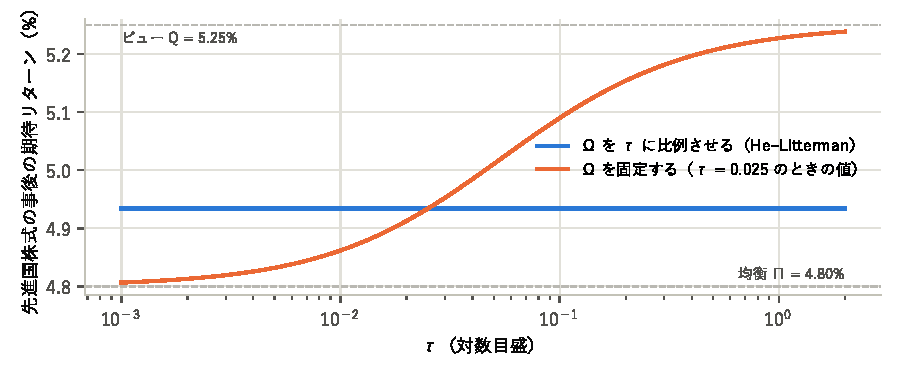
\includegraphics[width=0.92\linewidth]{fig_tau.pdf}
\caption{Idzorek の例で $\tau$ を動かしたときの、先進国株式の事後の期待リターン。$\Omega$ を $\tau$ に比例させると（青）一定、$\Omega$ を固定すると（橙）$\tau$ とともにビューへ近づく。}
\label{fig:tau}
\end{figure}

$\Omega$ を外から決める方法は多い。予想の誤差の分散、モデルの条件付き分散、LLM の回答のばらつきなどである（\chapref{ch:omega}）。そのどれでも、$\tau$ はビューの採用率を直接決める係数になる。本プロジェクトの $\tau=0.025$ も、そういう係数として働いている。

対象論文の第 2 版は、検証用の 3 か月で $\tau$ を選び直している。出発点の $\tau_{\mathrm{init}}$ は、$\Omega$ の平均と $\Sigma$ の平均の比である。1 資産で考えると、$\tau=\omega/\sigma^2$ なら採用率はちょうど 50\% になるので、$\tau_{\mathrm{init}}$ は「採用率がおよそ半分になる $\tau$」である。そこから 0.5〜1.5 倍の 5 点を試し、シャープレシオがいちばん高いものを使う。考え方は理解できるが、3 か月（隔週の見直しで約 6 回）の成績で選ぶと、偶然の当たり外れに合わせてしまうおそれが大きい。

\section{$\tau\approx1/T$ の意味}

過去 $T$ 期のリターンから平均を推定すると、その推定値の共分散は $\Sigma/T$ である。均衡リターンを「$T$ 期分のデータで推定した平均と同じくらい確か」とみなせば、$\tau\Sigma=\Sigma/T$、つまり $\tau=1/T$ になる。

\begin{center}
\small
\begin{tabular}{lll}
\toprule
$\tau$ & 年次のデータに直すと & 月次のデータに直すと \\
\midrule
0.05 & 20 年分 & 1 年 8 か月分 \\
0.025 & 40 年分 & 3 年 4 か月分 \\
0.01 & 100 年分 & 8 年 4 か月分 \\
1 & 1 年分 & 1 か月分 \\
\bottomrule
\end{tabular}
\end{center}

ここで、$\Sigma$ の期間（年次か月次か）によって読み方が変わることに注意する。$\tau=0.025$ は、年率の $\Sigma$ と組み合わせれば「40 年分の年次データと同じ確かさ」、月次の $\Sigma$ と組み合わせれば「40 か月分の月次データ」である。$\tau\Sigma$ の大きさ（期待リターンの不確かさの分散）は、どちらも同じで、年率に直すと標準偏差で $\sqrt{0.025}\times20\%\approx3.2\%$（市場の年率の標準偏差を 20\% とした場合）である。「均衡リターンの見込みが年率 ±3\% 程度は外れうる」という程度の確かさで、感覚的にも妥当な水準である。

$\tau=1$ は、均衡リターンが 1 期分のリターンと同じくらい不確かという意味で、年率なら「期待リターンは ±20\% 外れうる」と言っていることになる。均衡をほとんど信じない設定で、ビューが強く効く。

\section{$\tau$ と事後の共分散}

最適化で $\Sigma+M$ を使う場合、$\tau$ は比率の大きさにも効く。ビューがないとき $\Sigma+M=(1+\tau)\Sigma$ なので、比率は $\wmkt/(1+\tau)$ になる。$\tau=0.05$ なら 95.2\%、$\tau=1$ なら 50\% しか危険資産に投資しない。Meucci は、この「ビューのない事後が事前と一致しない」性質をパズルとして取り上げ、ビューを期待値ではなく実現値についてのものと読み替えた市場版の BL で解いた（\chapref{ch:hlmeucci}）。市場版では $\tau$ がそもそも出てこない。

\section{$\tau$ でトラッキングエラーを合わせる}\label{sec:tau-te}

Idzorek は、Lee（2000）が $\tau$ を 0.01〜0.05 に置いたうえで、目標のトラッキングエラー（ベンチマークからのずれの標準偏差）に合うように調整している、と紹介している。O'Toole（2017）も、$\tau$ は BL に暗黙に含まれるアクティブリスクの大きさと直接つながっており、目標のアクティブリスクから $\tau$ を決められる、と論じている。

$\Omega$ を固定して $\tau$ を動かせば、ビューの採用率が変わり、比率の傾きの大きさ（トラッキングエラー）が変わる。Idzorek の例で計算すると（\figref{fig:te} の左）、$\tau=0.025$ のときのトラッキングエラーは年率 \V{te.tau.base}\% で、2\% に合わせるには $\tau\approx\V{te.tau2}$ が必要になる。

この決め方の利点は、意味の分かりにくい $\tau$ を、運用で意味のある量（ずれの許容幅）に置き換えられることである。欠点は、「どれだけずれてよいか」と「ビューをどれだけ信じるか」を混ぜてしまうことである。ビューの当たり具合が悪いのに、許容幅が大きいからといって採用率を上げるのは筋が悪い。当たり具合は $\Omega$ で、ずれの許容幅は最適化の制約で、別々に決めるほうがよい（\chapref{ch:te}）。

\section{2 つの参照モデル}

Walters の整理では、BL の使い方には大きく 2 つの流儀がある。

\begin{description}[leftmargin=2em,style=nextline]
\item[標準的な参照モデル] $\mu$ を確率変数とし、$\mu\sim\mathcal N(\Pi,\tau\Sigma)$ を真面目に使う。事後の共分散 $\Sigma+M$ で最適化する。$\tau$ の大きさそのものが意味を持つので、慎重に決める必要がある。
\item[もう 1 つの参照モデル] 事後の期待リターンだけを使い、最適化には $\Sigma$ を使う。$\Omega$ を $\tau$ に比例させることが多く、その場合 $\tau$ は結果に効かない。
\end{description}

実務の多く（Idzorek、PyPortfolioOpt、本プロジェクト）は後者である。後者を使うなら、「$\tau$ は何がよいか」と悩む必要はほとんどない。悩むべきは $\Omega$（または、$\Omega$ を固定したときの $\tau\Sigma$ との比）である。

\begin{tipbox}[コツ：$\tau$ の決め方]
\begin{enumerate}
\item まず、$\Omega$ を何に比例させるかを決める。$\Omega$ を $\tau P\Sigma P\T$ に比例させるなら、$\tau$ はどの値でもよい（0.025 か 0.05 で十分）。
\item $\Omega$ を外から決める（誤差の分散、回答のばらつき、モデルの分散など）なら、$\tau$ は採用率を決める係数である。採用率が当たり具合に見合う大きさになるように、$\tau$（または $\Omega$ の倍率）を決める（\chapref{ch:accuracy}）。
\item 最適化で $\Sigma+M$ を使うなら、$\tau$ は比率の大きさにも効く。$\tau=1$ のような大きな値は避ける。
\item 少ない期間の成績で $\tau$ を選ばない。選んだ $\tau$ が、採用率としてどれくらいの値になっているかを確かめる。
\end{enumerate}
\end{tipbox}

\begin{keybox}[この章のまとめ]
\begin{itemize}
\item $\tau$ は、混ぜ方では $\Omega$ との比として、事後の共分散では大きさそのものとして効く。
\item $\Omega$ を $\tau$ に比例させると、事後の期待リターンから $\tau$ が消える。
\item $\Omega$ を外から決めると、$\tau$ が採用率を直接決める。本プロジェクトの $\tau=0.025$ はこの係数である。
\item $\tau\approx1/T$ は「均衡が何期分のデータと同じ確かさか」という読み方である。年率の $\Sigma$ で $\tau=0.025$ は、期待リターンの不確かさが年率で約 ±3\% という水準に当たる。
\end{itemize}
\end{keybox}


\part{ビューの不確かさ $\Omega$ の決め方}
% ============================================================
\chapter{$\Omega$ の決め方の全体像}\label{ch:omega}

$\Omega$ は、BL でいちばん抽象的で、いちばん結果を左右する入力である。Idzorek は、$\Omega$ の決め方には「誰にでも通じる答え」がない、という Litterman（2003）の言葉を引いている。Herold（2003）は、ビューごとに確率分布を決めなければならないことが BL の最大の難しさで、そのため BL は計量的な運用者にしか使えない、と述べている。

この章では、$\Omega$ の決め方を一覧にし、どれを選ぶときにも確かめるべき 3 つの点をまとめる。個々の方法は次の章から詳しく見る。

\section{$\Omega$ が表すもの}

$\Omega$ は、ビューの式 $P\mu=Q+\varepsilon$ の誤差 $\varepsilon$ の共分散である。言葉にすると「ビューの値 $Q$ が、本当の値 $P\mu$ からどれくらい外れうるか」である。対角成分 $\omega_k$ は $k$ 番目のビューの外れの大きさ（分散）、非対角成分は 2 つのビューの外れが同じ向きに出やすいかどうかを表す。

ここで「本当の値」が何を指すかで、$\Omega$ の大きさの意味が変わる。

\begin{itemize}
\item \textbf{元の BL}：ビューは期待リターン $\mu$ についてのもの。$\omega_k$ は「期待リターンの見込みの外れ」で、来期の実際のリターンの外れより小さい。
\item \textbf{Meucci の市場版}：ビューは来期に実現するリターン $r$ についてのもの。$\omega_k$ は「来期のリターンの予想の外れ」で、実現するリターンの散らばりまで含む（\chapref{ch:hlmeucci}）。
\end{itemize}

LLM や統計モデルの「来月のリターンの予想」は、ふつう後者である。予想の誤差を実際の結果と比べて測るなら、測れるのは後者の外れである。元の BL の式に入れるなら、実現値の散らばりの分を差し引いて考える必要がある（\chapref{ch:accuracy}）。

\section{決め方の一覧}

\begin{table}[htbp]
\centering
\caption{$\Omega$ の決め方。「$\tau$」の列は、その方法で $\tau$ が事後の期待リターンに効くかどうか。}
\label{tab:omega-methods}
\small
\begin{tabular}{p{2.3cm}p{3.3cm}p{0.8cm}p{4.0cm}p{1.8cm}}
\toprule
方法 & 式 & $\tau$ & 考え方・特徴 & 章・文献 \\
\midrule
He--Litterman & $\omega_k=\tau\,p_k\Sigma p_k\T$ & 消える & ビューと均衡を同じ重みで扱う。ビュー 1 つなら採用率 50\% & \ref{ch:hlmeucci}、He and Litterman 1999 \\
Meucci の確信度 & $\Omega=\frac1c P\Sigma P\T$ & --- & 市場版。ビューの誤差の相関を、ビューのポートフォリオの相関と同じとする & \ref{ch:hlmeucci}、Meucci 2010 \\
Idzorek の確信度 & $\omega_k=\tau p_k\Sigma p_k\T\frac{1-C_k}{C_k}$ & 消える & 0〜100\% の確信度から逆算。閉じた式は Walters による & \ref{ch:idzorek}、Idzorek 2007 \\
幅で決める & $\omega_k=(\text{幅の標準偏差})^2$ & 効く & 「$Q_k$ から ±$x$\% くらい外れうる」を分散に直す & \ref{ch:omega} \\
当たり具合（IC） & $\omega=\sigma^2(1/\IC^2-1)$ & --- & 過去の予想の当たり具合から決める。Grinold の式と同じ & \ref{ch:accuracy}、Grinold 1994 \\
誤差の分散 & $\omega=\Var(Q-r)-\text{実現値の散らばり}$ & 効く & 過去の予想の外れを直接測る & \ref{ch:accuracy} \\
モデルの予測分散 & 回帰の残差分散、GARCH の条件付き分散 & 効く & モデルが出す不確かさをそのまま使う。モデルの当たり具合の確認が要る & \ref{ch:macro}、Beach and Orlov 2007、Han and Li 2023 \\
回答のばらつき & 同じ質問への $N$ 個の回答の分散 & 効く & 対象論文の方法。当たり具合とは別物 & \ref{ch:text}、\ref{ch:project} \\
分布のエントロピー & $\omega=\omega_{\min}+(\omega_{\max}-\omega_{\min})H/\log3$ & 効く & 強気・中立・弱気の確率から & \ref{ch:text}、Florencio 2026 \\
複数の情報源の融合 & 精度加重、共分散の交差 & --- & 同じ資産への複数の予想をまとめる & \ref{ch:text}、Spears ほか 2023 \\
\bottomrule
\end{tabular}
\end{table}

\tabref{tab:omega-methods} の方法は、大きく 3 つに分けられる。

\begin{enumerate}
\item \textbf{比べる相手に合わせる}（He--Litterman、Meucci、Idzorek）：$\Omega$ を、均衡の不確かさや市場のボラティリティを基準にした倍率で決める。倍率を確信度という言葉で表す。何かの当たり具合を測っているわけではない。
\item \textbf{当たり具合を測る}（IC、誤差の分散）：過去の予想と実際の結果を比べて、外れの大きさを測る。データが必要だが、「どれだけ信じてよいか」に直接答える。
\item \textbf{作り方から出てくる不確かさを使う}（モデルの予測分散、回答のばらつき、エントロピー）：予想を作る道具が出す不確かさを使う。自動で決まるので便利だが、その不確かさが実際の外れと合っているかは別に確かめる必要がある。
\end{enumerate}

3 番目は、調査メモが「不確かさの内生化」「客観的な較正」と高く評価している方法である。しかし、道具が出す不確かさと実際の外れが合っている保証はない。本プロジェクトの LLM では、回答の分散は実際の外れの約 8 分の 1 だった（\chapref{ch:project}）。3 番目の方法を使うときは、2 番目の方法で確かめ、必要なら倍率を直す、という 2 段の手順にするのがよい。

\section{どの方法でも確かめる 3 つの点}

\begin{description}[leftmargin=2em,style=nextline]
\item[1. 単位] $\Omega$ と $\tau\Sigma$ は同じ単位（日次・月次・年率）で書かれているか。$Q$ が平均リターンなら、$\Omega$ も平均リターンの不確かさか。
\item[2. 大きさの基準] 1 つのビューの採用率は $s=\tau p\Sigma p\T/(\tau p\Sigma p\T+\omega)$ である。その値は、予想の当たり具合に見合っているか。He--Litterman の 50\% は、当たり具合とは関係なく決まった値である。
\item[3. 相関] $\Omega$ を対角にしてよいか。ビューの外れどうしに相関があるのに対角にすると、ビューの数だけ確信が積み上がる。
\end{description}

3 番目は見落とされやすい。次の節で例を挙げる。

\section{対角の $\Omega$ が確信を積み上げる}\label{sec:diag-trap}

同じ 1 つの情報源から、たくさんの資産についてのビューを作るとする。例えば、LLM に全銘柄の翌月のリターンを聞く。予想の外れには、銘柄ごとの部分と、全銘柄に共通する部分（「この月は全体に楽観的すぎた」）がある。共通する部分は、銘柄の数を増やしても平均で消えない。

ところが $\Omega$ を対角にすると、BL は外れが銘柄ごとに独立だと扱う。独立な外れは平均すると小さくなるので、「全銘柄の平均的な水準」についての確信は、銘柄の数に比例して強くなる。$K$ 個のビューが同じ大きさの独立な外れ $\omega$ を持つとき、その平均の外れの分散は $\omega/K$ である。$K=500$ なら 500 分の 1 である。実際の外れに共通部分があれば、この確信は根拠がない。

\begin{exbox}[本プロジェクトのデータでの例]
本プロジェクトの LLM の予想を、過去の当たり具合で較正して、1 銘柄だけなら採用率が 5〜7\% になるように $\Omega$ を置く（\chapref{ch:project}）。この $\Omega$ を対角にすると、約 490 銘柄を同時に入れたときの採用率は中央値で \V{bt.calib.adopt}\% になった。$\Omega$ を $\Sigma$ に比例させる（外れが市場と同じ相関を持つとする）と、採用率は設定どおり \V{bt.full.adopt}\% になった。
\end{exbox}

どれだけ積み上がるかは、\chapref{ch:stacking} で式にして確かめる。対策は 2 つある。

\begin{enumerate}
\item \textbf{$\Omega$ に相関を入れる}：Meucci の $\Omega=\frac1c P\Sigma P\T$ のように、外れの相関をビューのポートフォリオの相関と同じにする。$P=I$ なら $\Omega\propto\Sigma$ で、事後の期待リターンは $\Pi+s(Q-\Pi)$ と、すべての銘柄で同じ割合だけ動く。
\item \textbf{共通部分をビューから外す}：相対ビュー（銘柄どうしの差）や、平均を引いたビューにする。全体の水準についての見込みは、ビューに入れないか、別の 1 つのビューとして、それに見合った不確かさで入れる（\chapref{ch:shape}）。
\end{enumerate}

\section{選び方の流れ}

\begin{figure}[htbp]
\centering
\begin{tikzpicture}[node distance=5mm and 6mm,
  q/.style={draw=c1,fill=c1!8,rounded corners=2pt,align=center,font=\footnotesize,inner sep=3pt,text width=36mm,minimum height=9mm},
  a/.style={draw=c3,fill=c3!8,rounded corners=2pt,align=center,font=\footnotesize,inner sep=3pt,text width=38mm,minimum height=9mm}]
\node[q] (q1) {過去の予想と結果の\\記録があるか};
\node[a,right=16mm of q1] (a1) {IC・誤差の分散で較正\\（\chapref{ch:accuracy}）};
\node[q,below=of q1] (q2) {予想はモデルや LLM が\\自動で出すか};
\node[a,right=16mm of q2] (a2) {道具の不確かさを使い、\\記録がたまったら較正};
\node[q,below=of q2] (q3) {人の見方で、確信度を\\言葉で言えるか};
\node[a,right=16mm of q3] (a3) {Idzorek の確信度\\（\chapref{ch:idzorek}）};
\node[a,below=of q3] (a4) {He--Litterman（採用率 50\%）\\か、Meucci の $c$ で控えめに};
\node[q,right=16mm of a4,text width=44mm] (q4) {ビューが多いか（10 個以上）\\→ 相関を入れる、平均を外す};
\draw[arr] (q1) -- node[lab,above]{ある} (a1);
\draw[arr] (q1) -- node[lab,right]{ない} (q2);
\draw[arr] (q2) -- node[lab,above]{はい} (a2);
\draw[arr] (q2) -- node[lab,right]{いいえ} (q3);
\draw[arr] (q3) -- node[lab,above]{はい} (a3);
\draw[arr] (q3) -- node[lab,right]{いいえ} (a4);
\draw[arr,dashed] (a1.east) -- ++(5mm,0) |- (q4.east);
\end{tikzpicture}
\caption{$\Omega$ の決め方の選び方。どの方法を選んでも、ビューが多いときは相関の扱いを確かめる。}
\label{fig:omega-flow}
\end{figure}

\figref{fig:omega-flow} の考え方は、「測れるなら測る、測れないなら控えめに置く」である。確信度を言葉で決める方法は、測れないときの次善の策である。測れるデータがあるのに確信度を言葉で決めるのは、情報を捨てていることになる。

\begin{keybox}[この章のまとめ]
\begin{itemize}
\item $\Omega$ の決め方は、比べる相手に合わせるもの、当たり具合を測るもの、道具が出す不確かさを使うもの、の 3 つに分けられる。
\item どの方法でも、単位、大きさの基準（採用率）、相関の 3 点を確かめる。
\item ビューが多いのに $\Omega$ を対角にすると、共通の外れが無視され、確信が銘柄の数だけ積み上がる。相関を入れるか、共通部分をビューから外す。
\end{itemize}
\end{keybox}

% ============================================================
\chapter{Idzorek の確信度の方法}\label{ch:idzorek}

Idzorek の論文 \textit{A Step-by-Step Guide to the Black-Litterman Model: Incorporating User-Specified Confidence Levels}（初稿 2002 年、2004 年版、2007 年に Satchell 編の本の 1 章として出版）は、BL の入力の作り方を、8 資産の例で 1 段ずつ示した。いまも実務でいちばんよく参照される解説の 1 つである。この論文の新しい提案は、$\Omega$ を「0〜100\% の確信度」から決める方法である。

この章では、論文の例を表の数字どおりに再現し、確信度の方法が閉じた式になることを示す。そのうえで、論文では触れられていない注意点（ビューが複数あると、指定した確信度どおりには比率が動かない）を確かめる。

\section{例の設定}

例の資産は 8 つの資産クラスである。論文の表 5 の共分散（過去 60 か月の超過リターン）と、時価総額の比率を\tabref{tab:idz-inputs}に示す。

\begin{table}[htbp]
\centering
\caption{Idzorek の例の入力（年率 \%）。$\Pi$（論文）は論文の表 1 の値。右端は、論文の表から逆算した $\lambda=\V{idz.lam}$ で $\lambda\Sigma\wmkt$ を計算し直したもの。}
\label{tab:idz-inputs}
\tabin{idz_inputs}
\end{table}

論文は、市場のリスクプレミアム 3\% を市場の分散で割って $\lambda\approx3.07$ としている。逆算した $\lambda=\V{idz.lam}$ で $\Pi$ を計算し直すと、論文の表との差は最大 \V{idz.pidiff}\% で、表の丸めの範囲である。市場の標準偏差は \V{idz.mktsd}\%、期待超過リターンは \V{idz.mktprem}\% になる。

論文はまず、均衡以外の期待リターンを最適化に入れると何が起きるかを見せている。過去 60 か月の平均リターンを使うと、米国債券 1144\%、外国債券 $-105\%$、先進国株式 $-104\%$ という比率になる。回帰のベータの CAPM を使うと、均衡との相関は 99.8\% なのに、比率との相関は 66\% にとどまる。均衡リターン $\Pi$ を使えば、比率は時価総額の比率に戻る。

\section{3 つのビュー}

論文のビューは次の 3 つである。

\begin{enumerate}
\item 先進国株式（米国以外）の超過リターンは 5.25\% になる（確信度 25\%）。
\item 外国債券は米国債券を 0.25\% 上回る（確信度 50\%）。
\item 米国の大型・小型グロースは、米国の大型・小型バリューを 2\% 上回る（確信度 65\%）。
\end{enumerate}

\begin{table}[htbp]
\centering
\caption{3 つのビュー。$p_k\Pi$ は均衡が示すビューの値。$\omega^{\mathrm{HL}}$ は He--Litterman の $\tau p_k\Sigma p_k\T$（$\tau=0.025$）、$\omega^{\mathrm{Idz}}$ は確信度 $C_k$ から決めた値。}
\label{tab:idz-views}
\tabin{idz_views}
\end{table}

\tabref{tab:idz-views} の $p_k\Pi$ と $Q_k$ を比べると、ビューの「向き」が分かる。

\begin{itemize}
\item ビュー 1：均衡は \V{idz.ppi1}\%、ビューは 5.25\% なので、強気のビューである。
\item ビュー 2：均衡の差は \V{idz.ppi2}\%、ビューは 0.25\% なので、外国債券について\textbf{弱気}のビューである。言葉では「外国債券が上回る」だが、均衡が示す差より小さいので、比率は米国債券へ動く。
\item ビュー 3：均衡の差は \V{idz.ppi3}\%、ビューは 2\% なので、これもグロースについて\textbf{弱気}である。
\end{itemize}

ビューの言葉の向きと、比率が動く向きが逆になりうる。ビューは「均衡と比べてどうか」で効く、ということを忘れないようにしたい。

\subsection*{相対ビューの重みの付け方}

ビュー 3 は 4 つの資産を含む。$P$ の行の重みの付け方には 2 つの流儀がある。

\begin{itemize}
\item \textbf{等しい重み}（Satchell and Scowcroft 2000）：グロースの 2 資産に $+0.5$ ずつ、バリューの 2 資産に $-0.5$ ずつ。
\item \textbf{時価総額の重み}（Idzorek）：大型と小型の時価総額は 9 対 1 なので、$+0.9$、$+0.1$、$-0.9$、$-0.1$。
\end{itemize}

等しい重みでは、時価総額が 9 分の 1 しかない小型株の比率が大型株と同じだけ動き、意図しない大きなずれが生じる。Idzorek は時価総額の重みを勧めている。この資料の計算も時価総額の重みを使う。

\section{He--Litterman の $\Omega$ で計算する}

まず、He と Litterman の $\Omega=\diag(\tau p_k\Sigma p_k\T)$（$\tau=0.025$）で計算する。結果を\tabref{tab:idz-result}に示す。

\begin{table}[htbp]
\centering
\caption{事後の期待リターン $\mu$ と比率 $w$（年率 \%）。HL は He--Litterman の $\Omega$、Idz は Idzorek の確信度（25\%、50\%、65\%）から決めた $\Omega$、100\% は $\Omega=0$。比率は制約のない最適化 $w=(\lambda\Sigma)^{-1}\mu$。}
\label{tab:idz-result}
\tabin{idz_result}
\end{table}

HL の列は、論文の表 6 と、期待リターンで最大 \V{idz.erdiff}\%、比率で最大 \V{idz.wdiff}\% の差で一致する。読み取れることを挙げる。

\begin{itemize}
\item 期待リターンは 8 資産すべてで動くが、比率が動くのはビューのある 7 資産だけで、新興国株式は時価総額の比率のままである（\secref{sec:hl-property}）。
\item ビュー 1 は絶対ビューなので、比率の合計が \V{idz.wsum}\% になり、100\% を超える。全額投資の制約がある運用なら、絶対ビューは扱いに注意がいる。
\item 論文の表 8 の事前の指標も再現できる。BL の比率の標準偏差は \V{idz.blsd}\%、時価総額の比率からのずれ（アクティブリスク）は \V{idz.actrisk}\% である。ビューは比率を少ししか動かしていない。
\end{itemize}

\section{黙示の確信度}

Idzorek は、まず「いまの $\Omega$ は、確信度で言うと何 \% に当たるか」を測った。そのために、$\Omega=0$（100\% の確信）のときの比率 $w_{100\%}$ を計算し、
\begin{equation}
\text{黙示の確信度}=\frac{\hat w-\wmkt}{w_{100\%}-\wmkt}
\label{eq:implied-conf}
\end{equation}
を資産ごとに求める。100\% 信じたときの傾きに対して、実際には何割傾いたか、である。

He--Litterman の $\Omega$ では、3 つのビューの黙示の確信度は \V{idz.impl1}\%、\V{idz.impl2}\%、\V{idz.impl3}\% になる（論文では 32.94\%、43.06\%、33.02\%）。ビューを 1 つずつ入れた場合は、どのビューも 50\% である（\V{idz.single}）。ビューが 1 つなら、He--Litterman の $\Omega$ は「確信度 50\%」と同じだ、ということである。3 つ同時に入れると 50\% からずれるのは、ビューどうしが相関していて、互いの効き方に影響するからである。

いずれにせよ、ユーザーが言った確信度（25\%、50\%、65\%）は、He--Litterman の $\Omega$ では無視されている。Idzorek はこれを問題とし、確信度から $\Omega$ を決める方法を提案した。

\section{Idzorek の方法の手順}

ビュー $k$ ごとに、次の手順で $\omega_k$ を決める。

\begin{enumerate}
\item ビュー $k$ だけを 100\% 信じたときの期待リターン $\mu_{k,100\%}=\Pi+\tau\Sigma p_k\T(p_k\tau\Sigma p_k\T)^{-1}(Q_k-p_k\Pi)$ を計算する。
\item その比率 $w_{k,100\%}=(\lambda\Sigma)^{-1}\mu_{k,100\%}$ を計算する。
\item 100\% のときの傾き $D_{k,100\%}=w_{k,100\%}-\wmkt$ を求める。
\item 確信度 $C_k$ を掛けて、目標の傾き $C_k D_{k,100\%}$ を求める。
\item 目標の比率 $w_{k,\%}=\wmkt+C_kD_{k,100\%}$ を求める。
\item ビュー $k$ だけを $\omega_k$ で入れたときの比率 $w_k(\omega_k)$ が、目標の比率にもっとも近くなる $\omega_k$ を探す（差の 2 乗和を最小にする）。
\item すべてのビューの $\omega_k$ を並べて $\Omega$ を作り、BL の公式で事後の期待リターンを計算する。
\end{enumerate}

この手順では $\tau$ の値は結果に効かない。Idzorek はこれを利点として挙げている。

\section{閉じた式になる}\label{sec:idz-closed}

手順 6 は数値で探すように書かれているが、実は答えが式で書ける。ビュー $k$ だけを入れたとき、比率の傾きは式~\eqref{eq:hl-weights} から
\begin{equation}
w_k(\omega_k)-\wmkt=p_k\T\,\frac{\tau}{\lambda}\,\frac{Q_k-p_k\Pi}{\tau p_k\Sigma p_k\T+\omega_k}
\end{equation}
である。$\omega_k=0$ のときとの比は
\begin{equation}
\frac{w_k(\omega_k)-\wmkt}{w_{k,100\%}-\wmkt}=\frac{\tau p_k\Sigma p_k\T}{\tau p_k\Sigma p_k\T+\omega_k}
\end{equation}
で、ビューに含まれるすべての資産で同じ値になる。これが $C_k$ に等しくなるのは
\begin{equation}
\boxed{\;\omega_k=\tau\,p_k\Sigma p_k\T\cdot\frac{1-C_k}{C_k}\;}
\label{eq:idz-closed}
\end{equation}
のときである。目標の比率にちょうど一致するので、手順 6 の差の 2 乗和は 0 になる。この式は Walters の解説（2014）にあり、PyPortfolioOpt の Idzorek の方法も、Walters の閉じた式を使うと説明している。

\begin{exbox}[数値で確かめる]
論文の手順 6 のとおりに数値で $\omega_k$ を探すと、式~\eqref{eq:idz-closed} との差は最大 \V{idz.omnumdiff}\% だった。$\omega_k$ は\tabref{tab:idz-views}の右端の列で、He--Litterman の値と比べると、ビュー 1（確信度 25\%）は \V{idz.omratio1} 倍、ビュー 2（50\%）は \V{idz.omratio2} 倍、ビュー 3（65\%）は \V{idz.omratio3} 倍である。確信度 50\% が He--Litterman と同じになることも確かめられる。
\end{exbox}

式~\eqref{eq:idz-closed} から分かることを挙げる。

\begin{itemize}
\item $C_k$ は、ビューが 1 つのときの採用率 $s$ そのものである（式~\eqref{eq:adoption}）。Idzorek の確信度は「均衡からビューへ何割動かしたいか」を直接言っていることになる。
\item $C_k=50\%$ は He--Litterman と同じ。$C_k\to100\%$ で $\omega_k\to0$、$C_k\to0$ で $\omega_k\to\infty$。
\item $\omega_k$ は $\tau$ に比例するので、$\tau$ は消える。
\end{itemize}

\section{ビューが複数あると、確信度どおりには動かない}\label{sec:idz-multi}

手順 1〜6 は、ビューを 1 つずつ扱っている。手順 7 で 3 つを同時に入れたとき、それぞれのビューの傾きは確信度どおりになるだろうか。式~\eqref{eq:implied-conf} で確かめた結果を\tabref{tab:idz-conf}に示す。

\begin{table}[htbp]
\centering
\caption{黙示の確信度。「1 つだけ」はビューを 1 つずつ入れた場合、「3 つ同時」はすべてを入れた場合。分母の 100\% の傾きは、それぞれ同じ条件（1 つだけ、3 つ同時）で $\Omega=0$ にしたもの。}
\label{tab:idz-conf}
\tabin{idz_conf}
\end{table}

\begin{figure}[htbp]
\centering
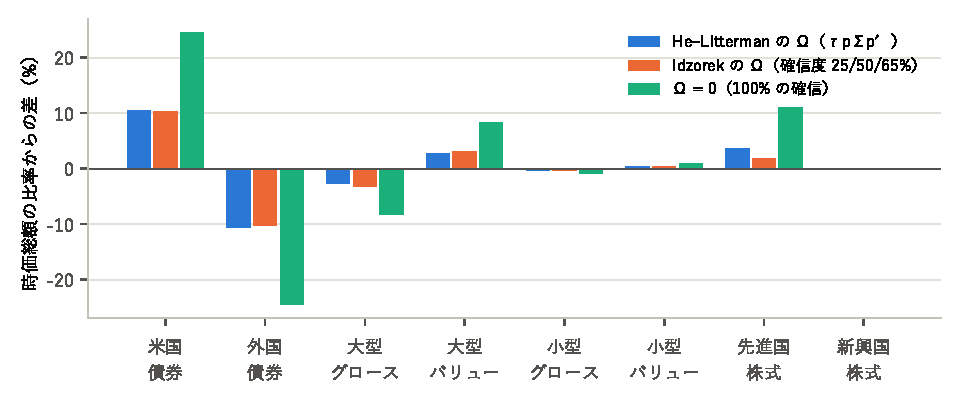
\includegraphics[width=0.95\linewidth]{fig_idz_tilts.pdf}
\caption{3 つのビューを同時に入れたときの、時価総額の比率からの差。Idzorek の $\Omega$（確信度 25/50/65\%）でも、傾きは 100\% のときの 25/50/65\% にはならない。}
\label{fig:idz-tilts}
\end{figure}

3 つを同時に入れると、確信度 25\% のビュー 1 は \V{idz.ach1}\%、50\% のビュー 2 は \V{idz.ach2}\%、65\% のビュー 3 は \V{idz.ach3}\% しか傾かなかった（\figref{fig:idz-tilts}）。指定どおりにならない理由は、事後の式の $(P\tau\Sigma P\T+\Omega)^{-1}$ にある。ビューのポートフォリオどうしが相関していると、この逆行列の非対角成分を通じて、あるビューの驚きが別のビューの傾きを打ち消したり強めたりする。例では、先進国株式（ビュー 1）とグロース・バリューの差（ビュー 3）がどちらも株式で、共分散を持つ。

これは Idzorek の方法の誤りではない。論文は、確信度を「ビューごとの傾きの目安」として決める方法を提案しており、組み合わせたときの傾きまでは約束していない。ただ、利用者は「65\% と言ったのだから 65\% 動く」と考えがちなので、注意がいる。

3 つ同時の傾きを確信度に合わせたいなら、3 つの $\omega_k$ をまとめて探す方法が考えられる。この例で探すと、$\omega=(\V{idz.omjoint1},\ \V{idz.omjoint2},\ \V{idz.omjoint3})\times10^{-4}$ で、3 つのビューの傾きはそれぞれ \V{idz.achj1}\%、\V{idz.achj2}\%、\V{idz.achj3}\% になった（目標との差の最大は \V{idz.joint.res}）。ビュー 3 の $\omega$ はほぼ 0、つまり 100\% の確信まで上げても、傾きは 65\% に届かなかった。ほかのビューとの相関に打ち消されるためで、確信度の組み合わせによっては、3 つを同時に合わせることはできない。

そもそも、確信度は「ビューをどれだけ信じるか」であって、「比率をどれだけ動かすか」ではない。後者に無理に合わせると、相関によって打ち消し合うビューの確信を、根拠なく高く置くことになる（例では 100\% にまで上がった）。比率の動きを確信度に合わせることにこだわらず、確信度は 1 つずつの採用率として決め、組み合わせたときの動きは黙示の確信度で確かめるのがよい。

\section{確信度をどう決めるか}

Idzorek は、確信度を決める材料として、ビューを作ったモデルや分析者の過去の当たり具合、ビューと均衡の差の大きさなどを挙げている。さらに、複数の分析者からビューを集めるなら、それぞれの情報係数（IC、予想と実際の相関）に応じて確信度を決めれば、腕のよい分析者を重く扱える、と述べている（Grinold and Kahn 1999 の IC）。

ここで、確信度を当たり具合から決めると、どんな数字になるかを先に見ておく（詳しくは \chapref{ch:accuracy}）。予想と実際のリターンの相関が IC のとき、予想に合わせて期待リターンを動かすべき割合は、おおよそ $\IC^2$ である。IC は、腕のよい運用者でも 0.05〜0.10 程度とされる（『総合報告書』の Grinold の式の節）。つまり、当たり具合に見合う確信度は 0.25〜1\% である。人が言葉で選ぶ 25\%、50\%、65\% は、当たり具合の点では 2 桁大きい。

\begin{notebox}[確信度の言葉と、当たり具合の数字]
「65\% 確信している」という言葉は、多くの人にとって「かなり自信がある」程度の意味である。しかし BL の確信度は「均衡からビューへ 65\% 動かす」という意味になる。来月のリターンの予想で、均衡から 65\% 動かしてよいほど当たる予想は、ほとんどない。確信度を言葉で決めるときは、その値が採用率として妥当かを、当たり具合の数字（IC）と照らし合わせるとよい。
\end{notebox}

\section{結果を確かめて調整する}

Idzorek は、計算した比率と期待リターンを見て、$\tau$ や $\omega_k$ を調整する「微調整」も勧めている。その目安として、Bevan と Winkelmann（1998）の経験則を紹介している。BL の比率の事前の情報レシオ（超過リターン ÷ アクティブリスク）を計算し、2.0 を超えていたら、ビューの重みを下げる（$\tau$ を下げる）。例の BL の比率の事前の情報レシオは 0.07 程度で、目安を大きく下回る。

情報レシオ 2.0 は、上限としてはかなり緩い。事後の情報レシオが 0.5 を超える運用は優秀とされる。事前の情報レシオが 1 を大きく超えるなら、ビューを信じすぎていないか疑うほうがよい（\chapref{ch:te}）。

\begin{tipbox}[コツ：Idzorek の方法を使うとき]
\begin{enumerate}
\item 確信度 $C_k$ は、ビューが 1 つのときの採用率である。閉じた式 $\omega_k=\tau p_k\Sigma p_k\T(1-C_k)/C_k$ で計算すればよく、数値で探す必要はない。
\item ビューの向きは、言葉ではなく均衡との差で決まる。$Q_k$ と $p_k\Pi$ を並べて確かめる。
\item 相対ビューの重みは時価総額で付ける。等しい重みは小さい資産を大きく動かす。
\item ビューが複数あると、比率は確信度どおりには動かない。黙示の確信度を計算して確かめる。
\item 確信度を言葉で決めるときは、当たり具合（IC の 2 乗）と比べて大きすぎないかを確かめる。
\end{enumerate}
\end{tipbox}

\begin{keybox}[この章のまとめ]
\begin{itemize}
\item Idzorek の 8 資産の例は、論文の表の数字どおりに再現できる。
\item 確信度の方法は、閉じた式 $\omega_k=\tau p_k\Sigma p_k\T(1-C_k)/C_k$ と同じで、$C_k$ はビュー 1 つのときの採用率である。
\item 3 つのビューを同時に入れると、確信度 25/50/65\% のビューは \V{idz.ach1}/\V{idz.ach2}/\V{idz.ach3}\% しか動かなかった。ビューの相関が互いの効き方を変えるためである。
\item 当たり具合から見ると、妥当な確信度は 1\% 前後で、言葉で選ぶ値より 2 桁小さい。
\end{itemize}
\end{keybox}

% ============================================================
\chapter{He--Litterman の $\Omega$ と Meucci の流儀}\label{ch:hlmeucci}

この章では、比べる相手に合わせて $\Omega$ を決める 2 つの流儀を扱う。He と Litterman（1999）の $\Omega=\tau\diag(P\Sigma P\T)$ と、Meucci（2005、2010）の $\Omega=\frac1c P\Sigma P\T$ である。後者は、ビューを「期待リターン」ではなく「実現するリターン」についてのものと読み替えた「市場版の BL」と組になっている。LLM や統計モデルの予想は実現するリターンの予想なので、市場版の考え方はこの資料の後半で何度も使う。

\section{He--Litterman の $\Omega$}

He と Litterman は、ビューの不確かさを、ビューのポートフォリオの分散に比例させた。
\begin{equation}
\Omega=\diag\bigl(P\,\tau\Sigma\,P\T\bigr),\qquad \omega_k=\tau\,p_k\Sigma p_k\T
\label{eq:hl-omega}
\end{equation}
この置き方の意味は、「ビューの見込みの外れは、均衡の見込みの外れと同じくらい」である。ビューが 1 つなら採用率は 50\%、ビューと均衡のちょうど中間をとる。

この置き方の利点は 3 つある。

\begin{enumerate}
\item $\tau$ が消える（\secref{sec:tau-cancel}）。
\item ビューのポートフォリオのリスクが大きいほど、ビューの不確かさも大きくなる。ボラティリティの高い資産の 1\% と、低い資産の 1\% を同じ重みで扱わずに済む。
\item 単位を気にしなくてよい。$\Sigma$ と同じ単位で $\Omega$ が決まる。
\end{enumerate}

欠点は、当たり具合とまったく関係がないことである。予想がほとんど当たらなくても、よく当たっても、採用率は 50\% になる。He と Litterman の論文の目的は、BL の比率の形を直感的に説明することで、$\Omega$ の値を正しく決めることではなかった。この置き方は、説明のための「中立な既定値」と考えるのがよい。

\section{Meucci の確信度 $c$}

Meucci は $\Omega$ を、ビューのポートフォリオの共分散全体に比例させた。
\begin{equation}
\Omega=\frac1c\,P\Sigma P\T
\label{eq:meucci-omega}
\end{equation}
$c\in(0,\infty)$ は、ビュー全体への確信の度合いである。He--Litterman との違いは 2 つある。

\begin{itemize}
\item \textbf{非対角を残す}：$P\Sigma P\T$ の非対角成分（ビューのポートフォリオどうしの共分散）をそのまま使う。ビューの外れが、ビューのポートフォリオと同じように相関する、という仮定である。
\item \textbf{$\tau$ を含まない}：市場版の BL（次の節）と組み合わせるので、比べる相手は $\tau\Sigma$ ではなく $\Sigma$ そのものである。$c=1$ なら「ビューの外れは、市場の 1 期分の散らばりと同じくらい」となる。
\end{itemize}

ビューごとに確信の度合いを変えたいときは、
\begin{equation}
\Omega=\frac1c\,\diag(u)\,P\Sigma P\T\,\diag(u)
\label{eq:meucci-u}
\end{equation}
とする。$u_k$ が大きいビューほど不確かである。

\subsection*{言葉のビューを数字に直す}

Meucci は、「強気」「弱気」のような言葉だけのビューを数字に直す方法も示している。
\begin{equation}
v_k=(P\pi)_k+\eta_k\sqrt{(P\Sigma P\T)_{kk}},\qquad \eta_k\in\{-\beta,-\alpha,+\alpha,+\beta\}
\label{eq:meucci-eta}
\end{equation}
$\eta_k$ は「とても弱気」「弱気」「強気」「とても強気」を表し、典型的には $\alpha=1$、$\beta=2$ である。つまり、ビューの値を「均衡から、ビューのポートフォリオの標準偏差の何倍ずれるか」で決める。

この置き方は、ビューの大きさをボラティリティで測るので、資産によって大きさの感覚が変わらない。ただし、$\alpha=1$ は「1 標準偏差」で、1 年のリターンの予想としてはかなり大きい（年率 20\% の株式なら 20\%）。ビューの大きさは、当たり具合に合わせて小さく取るのが安全である（\chapref{ch:accuracy}）。

\section{市場版の BL：ビューを実現値についてのものとみる}

Meucci は、元の BL の事後分布に 2 つの「パズル」があると指摘した。

\begin{enumerate}
\item ビューをまったく信じないとき（$\Omega\to\infty$）、事後の予測分布は $\mathcal N(\pi,(1+\tau)\Sigma)$ になり、事前の市場のモデル $\mathcal N(\pi,\Sigma)$ に戻らない。
\item ビューを 100\% 信じても（$\Omega\to0$）、事後の予測の共分散は $\Sigma$ の部分を残し、決して退化しない。ビューの方向にも散らばりが残る。
\end{enumerate}

どちらも、元の BL ではビューが期待値 $\mu$ についてのもので、実現値の散らばり $\Sigma$ には触れないことから来ている。理屈としては一貫しているが、実務家の直感とは合わない。

Meucci は、ビューを市場の実現値 $X$ そのものについてのものとみる版を示した。$\mu$ を確率変数とせず $\mu=\pi$ とし、
\begin{equation}
X\sim\mathcal N(\pi,\Sigma),\qquad V\mid x\sim\mathcal N(Px,\Omega)
\end{equation}
とする。ビューの値 $v$ を観測したときの $X$ の事後分布は、正規分布の条件付けで求まる（\appref{app:formulas}）。
\begin{align}
\mu_{\mathrm{mBL}}&=\pi+\Sigma P\T\bigl(P\Sigma P\T+\Omega\bigr)^{-1}(v-P\pi)\label{eq:mbl-mu}\\
\Sigma_{\mathrm{mBL}}&=\Sigma-\Sigma P\T\bigl(P\Sigma P\T+\Omega\bigr)^{-1}P\Sigma\label{eq:mbl-sigma}
\end{align}
元の BL の更新形と比べると、$\tau\Sigma$ が $\Sigma$ に置き換わっただけである。違いは次のとおりである。

\begin{itemize}
\item $\tau$ が出てこない。
\item 事後の共分散に $\Sigma$ を足す必要がない。
\item $\Omega\to\infty$ で事前 $\mathcal N(\pi,\Sigma)$ に戻り、$\Omega\to0$ で正規分布の条件付き分布（シナリオ分析）になる。
\end{itemize}

\section{Meucci の 6 か国の例}

Meucci の論文の例は、6 か国の株価指数（イタリア、スペイン、スイス、カナダ、アメリカ、ドイツ）である。年率の標準偏差、相関、時価総額の比率が論文に載っている。$\lambda=1.2$ で $\pi=2\lambda\Sigma w$ を計算すると、$\pi=(\V{meu.pi})\%$ になる（論文は約 6、7、9、8、17、10\%。入力が丸められているため、スイスは少し違う）。論文は $\tau=0.4$ を使う。ビューは次の 2 つで、確信度は $c=1$（$\Omega=P\Sigma P\T$）である。

\begin{enumerate}
\item スペインの指数は年率 12\% 上がる（均衡は \V{meu.ppi1}\%）。
\item アメリカとドイツの差は年率 $-10\%$ になる（均衡は \V{meu.ppi2}\%）。
\end{enumerate}

\begin{table}[htbp]
\centering
\caption{Meucci の 6 か国の例（年率 \%）。$\mu_{\mathrm{BL}}$、$\sigma_{\mathrm{BL}}$ は元の BL（$\tau=0.4$、共分散は $\Sigma+M$）、$\mu_{\mathrm{mBL}}$、$\sigma_{\mathrm{mBL}}$ は市場版。$w^*$ は空売りなし・全額投資で $w\T\mu-\lambda w\T\Sigma w$（$\lambda=1.2$）を最大にした比率。}
\label{tab:meucci}
\tabin{meucci}
\end{table}

\tabref{tab:meucci} から分かることを挙げる。

\begin{itemize}
\item スペインの期待リターンは、元の BL で \V{meu.blspain}\%、市場版で \V{meu.mspain}\% になる。同じ $\Omega$ でも、比べる相手が $\tau\Sigma$（元の BL）か $\Sigma$（市場版）かで、採用率が違う。$\tau=0.4<1$ なので元の BL のほうが均衡寄りである。
\item 標準偏差は、元の BL では $\Sigma+M$ で大きくなり、市場版ではビューの分だけ小さくなる。
\item 市場版の比率は、スペインとドイツが増え、アメリカが減る。Meucci の論文の図（スペインは低リスクの側で増え、ドイツはどのリスク回避度でも増え、アメリカは減る）と同じ向きである。
\item 元の BL（共分散は $\Sigma+M$）では、アメリカが減った分がほかの国に広く分かれ、ドイツはほとんど変わらない。同じビューでも、比べる相手と最適化に使う共分散で、比率の動き方は変わる。
\end{itemize}

\subsection*{100\% 信じたとき}

$\Omega\to0$ にすると、スペインの期待リターンは、元の BL でも市場版でも \V{meu.full.bl}\%（ビューの値そのもの）になる。違うのは標準偏差で、元の BL では \V{meu.full.blsd}\% のまま、市場版では \V{meu.full.msd}\%（スペインの値が確定する）になる。ビューをまったく信じないとき、元の BL のスペインの標準偏差は $\sqrt{1+\tau}$ 倍の \V{meu.unc.blsd}\% になり、事前の 24.0\% に戻らない。Meucci の言う 2 つのパズルが、数字で確かめられる。

\subsection*{言葉のビュー}

\begin{table}[htbp]
\centering
\caption{Meucci の式~\eqref{eq:meucci-eta} で、言葉のビューを数字に直したもの（年率 \%、$\alpha=1$、$\beta=2$）。}
\label{tab:meucci-eta}
\tabin{meucci_eta}
\end{table}

\tabref{tab:meucci-eta} のとおり、「強気」のスペインは $\V{meu.ppi1}+\V{meu.vsd1}$\% になる。1 標準偏差は、1 年の期待リターンのずれとしては大きい。このまま $c=1$ で入れると、ビューの影響はかなり強く出る。

\section{どちらを使うか}

\begin{center}
\small
\begin{tabular}{p{2.6cm}p{5.2cm}p{5.2cm}}
\toprule
 & 元の BL & 市場版の BL \\
\midrule
ビューの対象 & 期待リターン $\mu$ & 来期に実現するリターン $X$ \\
比べる相手 & $\tau\Sigma$ & $\Sigma$ \\
$\tau$ & 必要（$\Omega\propto\tau$ なら消える） & 不要 \\
最適化の共分散 & $\Sigma$ または $\Sigma+M$ & $\Sigma_{\mathrm{mBL}}$ \\
向いているビュー & 長い期間の期待リターンの見込み（「この 5 年の平均はこうだろう」） & 来期の予想（「来月はこうなるだろう」）、シナリオ \\
$\Omega$ を測るには & 期待値の外れなので、実現値と比べるときは実現値の散らばりを差し引く & 実現値と比べた予想の外れをそのまま使える \\
\bottomrule
\end{tabular}
\end{center}

LLM の「翌月の日次の平均リターン」の予想は、来期の実現値の予想である。過去の予想と実際の結果を比べて測った外れは、そのまま市場版の $\Omega$ になる。元の BL の式を使い続ける場合は、実現値の散らばりの分を差し引いてから $\Omega$ にするか、$\tau$ を「1 か月の平均の散らばり」に合わせて読み替える必要がある（\chapref{ch:accuracy}）。

\begin{tipbox}[コツ：比べる相手を意識する]
\begin{itemize}
\item He--Litterman の $\Omega$ は採用率 50\% の既定値で、当たり具合とは関係がない。説明や比較の出発点として使い、運用の値としては見直す。
\item 予想の外れを実際の結果で測るなら、ビューは実現値についてのもので、市場版の式（$\tau$ なし）が自然である。
\item ビューが多いときは、Meucci の $\Omega=\frac1c P\Sigma P\T$ のように非対角を残すと、確信の積み上がりを防げる。
\end{itemize}
\end{tipbox}

\begin{keybox}[この章のまとめ]
\begin{itemize}
\item He--Litterman の $\Omega=\tau\diag(P\Sigma P\T)$ は、ビュー 1 つなら採用率 50\% の中立な既定値である。
\item Meucci の $\Omega=\frac1cP\Sigma P\T$ は、ビューの外れに相関を持たせ、市場版の BL と組になる。
\item 市場版の BL は、ビューを来期の実現値についてのものとみる。$\tau$ が不要で、ビューを信じないときは事前に、100\% 信じるときは条件付き分布に、それぞれ一致する。
\end{itemize}
\end{keybox}

% ============================================================
\chapter{予想の当たり具合から $\Omega$ を決める}\label{ch:accuracy}

ここまでの方法（He--Litterman、Meucci、Idzorek）は、$\Omega$ を何かとの比で決めていた。この章では、$\Omega$ を予想の当たり具合から決める。過去の予想と実際の結果の記録があれば、「どれだけ信じてよいか」はデータで答えられる。

中心になる結果は次のとおりである。Meucci の市場版の BL で、ビューの不確かさを $\omega=\sigma^2(1/\IC^2-1)$ と置くと、事後の期待リターンは Grinold の式 $\alpha=\IC\cdot\sigma\cdot z$ とちょうど一致する。運用の実務で昔から使われている「予想を当たり具合で縮める」式と、BL は同じものだということである。

\section{当たり具合を測る 3 つの量}

予想 $q_i$ と、その後に実現したリターン $r_i$ の組（銘柄 $i=1,\dots,N$、時点 $t=1,\dots,T$）があるとする。当たり具合の測り方は 3 つある。

\begin{description}[leftmargin=2em,style=nextline]
\item[情報係数（IC）] 予想と実際の相関 $\IC=\mathrm{corr}(q,r)$。順位相関で測ることも多い。大きさの単位によらない。
\item[較正の傾き $b$] 実際を予想に回帰したときの傾き $b=\Cov(q,r)/\Var(q)$。予想の大きさまで含めた当たり具合で、$b=\IC\cdot\sigma_r/\sigma_q$ の関係がある。
\item[誤差の 2 乗の平均（MSE）] $\E[(q-r)^2]$。予想の外れの大きさそのもの。
\end{description}

$b=1$ なら、予想の大きさはちょうどよい。$b<1$ なら予想は大きすぎ（自信過剰）、$b>1$ なら小さすぎ（控えめすぎ）、$b<0$ なら向きが逆である。BL に入れるときに必要なのは、この 3 つのうち $b$（または IC と、予想と実際の散らばりの比）である。

\section{Grinold の式}

Grinold（1994）は、予想の点数を期待リターンに直す式として、
\begin{equation}
\alpha_i=\IC\cdot\sigma_i\cdot z_i
\label{eq:grinold}
\end{equation}
を示した（論文の題名は \textit{Alpha is Volatility Times IC Times Score}）。$z_i$ は銘柄 $i$ の点数を平均 0、標準偏差 1 にそろえたもの、$\sigma_i$ はその銘柄のリターンの標準偏差（ここでは特異リスクに限らず、予想する期間のリターンの標準偏差とする）、$\alpha_i$ は期待リターンの、市場の見込みからのずれである。

この式は、予想 $q$ と実際 $r$ が 2 変量正規分布に従うときの条件付き期待値そのものである。
\begin{equation}
\E[r\mid q]=\E[r]+\mathrm{corr}(q,r)\,\sigma_r\,\frac{q-\E[q]}{\sigma_q}=\E[r]+\IC\cdot\sigma_r\cdot z
\end{equation}
つまり Grinold の式は、「予想を見たあとで、実現するリターンの平均はどうなるか」を、回帰で答えたものである。予想がほとんど当たらないなら（IC が小さいなら）、期待リターンはほとんど動かない。

IC は、優れた運用者でも 0.05 前後とされる。月次の標準偏差が 8\% の銘柄なら、点数が 1 標準偏差高い銘柄の期待リターンは $0.05\times8\%=0.4\%$ しか上がらない。

\section{市場版の BL と Grinold の式は同じ}\label{sec:grinold-bl}

市場版の BL（\chapref{ch:hlmeucci}）で、1 資産・1 ビューの場合を考える。来期のリターン $x$ は $\mathcal N(\pi,\sigma^2)$ に従い、ビュー $v$ は $x$ に外れ $\varepsilon\sim\mathcal N(0,\omega)$ が乗ったもの、つまり $v=x+\varepsilon$ とする。事後の期待値は、式~\eqref{eq:mbl-mu} から
\begin{equation}
\E[x\mid v]=\pi+\frac{\sigma^2}{\sigma^2+\omega}(v-\pi)
\label{eq:mbl-scalar}
\end{equation}
である。この設定で予想 $v$ と実際 $x$ の相関を計算すると、$\Cov(v,x)=\sigma^2$、$\Var(v)=\sigma^2+\omega$ なので、
\begin{equation}
\IC=\mathrm{corr}(v,x)=\frac{\sigma}{\sqrt{\sigma^2+\omega}},\qquad
\IC^2=\frac{\sigma^2}{\sigma^2+\omega}
\end{equation}
となる。式~\eqref{eq:mbl-scalar} の採用率は、ちょうど $\IC^2$ である。逆に解くと
\begin{equation}
\boxed{\;\omega=\sigma^2\Bigl(\frac{1}{\IC^2}-1\Bigr)\;}
\label{eq:omega-ic}
\end{equation}
である。さらに、予想を標準化した点数 $z=(v-\pi)/\sqrt{\sigma^2+\omega}=(v-\pi)\,\IC/\sigma$ を使うと、
\begin{equation}
\E[x\mid v]-\pi=\IC^2\,(v-\pi)=\IC^2\cdot\frac{\sigma z}{\IC}=\IC\cdot\sigma\cdot z
\end{equation}
となり、Grinold の式~\eqref{eq:grinold} と一致する。

\begin{thmbox}[市場版の BL と Grinold の式]
予想の外れの分散を $\omega=\sigma^2(1/\IC^2-1)$ と置いた市場版の BL の事後の期待リターンは、Grinold の式 $\pi+\IC\cdot\sigma\cdot z$ に等しい。このときの採用率は $\IC^2$ である。
\end{thmbox}

\begin{table}[htbp]
\centering
\caption{IC と、それに見合う採用率・$\omega$。「生の予想の広がり」は、$v=x+\varepsilon$ の設定で予想の標準偏差が実際の何倍か。右端は、月次の標準偏差 8\% の銘柄で、点数が 1 標準偏差高いときの期待リターンの上乗せ（月次 \%）。}
\label{tab:ic}
\tabin{ic}
\end{table}

\tabref{tab:ic} のとおり、IC が 0.05 なら採用率は 0.25\%、$\omega$ は $\sigma^2$ の 399 倍である。He--Litterman の採用率 50\% は IC で言えば 0.71 に当たる。来月のリターンを予想して IC が 0.7 になることは、まずない。

\subsection*{シミュレーションで確かめる}

$v=x+\varepsilon$ の設定で、IC が 0.10 になるように \V{sim.n} 組の $(x,v)$ を作った（\figref{fig:ic-sim}）。実際の IC は \V{sim.ic} である。

\begin{figure}[htbp]
\centering
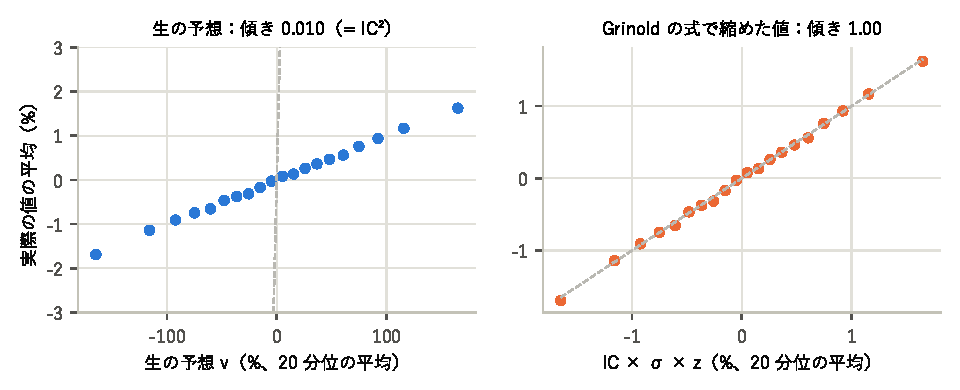
\includegraphics[width=0.95\linewidth]{fig_ic_sim.pdf}
\caption{予想の 20 分位ごとの、実際の値の平均。左：生の予想 $v$ は、実際の値に対して大きすぎる（傾き $\approx\IC^2$）。右：Grinold の式で縮めた値は、実際の値と傾き 1 で並ぶ。破線は 45 度の線。}
\label{fig:ic-sim}
\end{figure}

生の予想 $v$ に対する実際の値の傾きは \V{sim.slope.raw} で、$\IC^2=0.01$ に一致する。生の予想を期待リターンとしてそのまま使うと、100 倍の自信過剰になる。Grinold の式で縮めた値の傾きは \V{sim.slope.post} で、ほぼ 1 である。BL の言葉で言えば、正しい採用率で混ぜると、予想は「較正された」状態になる。

\section{元の BL に直す}

元の BL（$\tau$ を使う形）で同じ採用率にするには、$\tau\sigma^2/(\tau\sigma^2+\omega)=\IC^2$ から
\begin{equation}
\omega=\tau\sigma^2\Bigl(\frac{1}{\IC^2}-1\Bigr)
\label{eq:omega-ic-tau}
\end{equation}
と置けばよい。Idzorek の確信度で言えば $C=\IC^2$ である。この $\omega$ は $\tau$ に比例するので、$\tau$ は消える。

ここで注意が 1 つある。式~\eqref{eq:omega-ic} と式~\eqref{eq:omega-ic-tau} は、1 資産・1 ビューで採用率を合わせたものである。ビューが多く、$\Omega$ を対角にすると、ビューの相関を通じて採用率が変わる（\secref{sec:diag-trap}）。複数のビューで「どの銘柄も同じ割合 $s$ だけ動かす」には、$\Omega$ を $\Sigma$ に比例させる。
\begin{equation}
\Omega=\tau\Bigl(\frac1s-1\Bigr)P\Sigma P\T\quad\Longrightarrow\quad
\muBL=\Pi+s\,\Sigma P\T(P\Sigma P\T)^{-1}(Q-P\Pi)
\label{eq:omega-prop}
\end{equation}
$P=I$（すべての銘柄に絶対ビュー）なら $\muBL=\Pi+s(Q-\Pi)$ で、すべての銘柄が同じ割合だけビューへ動く。

\section{較正の傾きで測る}\label{sec:slope}

実際には、IC と予想の大きさ（予想の標準偏差）は別々にずれる。LLM の予想のように、予想の散らばりが実際の散らばりと無関係に決まっている場合、IC だけで縮めても大きさが合わない。このときは、較正の傾き $b$ を直接測り、それを採用率にするのが簡単である。

\begin{enumerate}
\item 時点ごとに、予想 $q_{it}$ と実際 $r_{it}$ から、その時点の平均を引く（全体の水準の当たり外れを除き、銘柄間の差だけを見る）。
\item すべての時点をまとめて、実際を予想に回帰した傾き $b=\sum_{i,t}\tilde q_{it}\tilde r_{it}\big/\sum_{i,t}\tilde q_{it}^2$ を求める（$\tilde{}$ は平均を引いたもの）。
\item 判断日より前の時点だけで $b$ を計算する（先読みしない）。データがないうちは $b=0$（均衡のまま）とする。
\item $b$ を 0 から 1 の範囲に収め、式~\eqref{eq:omega-prop} の $s$ として使う。$b\le0$ なら、ビューは使わない。
\end{enumerate}

本プロジェクトの LLM の予想で計算すると、月ごとの傾きの平均は \V{llm.slope.mean}（$t$ 値 \V{llm.slope.t}）、30 か月をまとめた傾きは \V{llm.slope.pooled} だった（\chapref{ch:project}）。予想の散らばりのうち、実際の差につながっているのは 7\% 程度で、残りは雑音である。

\subsection*{推定の誤差}

$b$ や IC も推定値なので、誤差がある。月ごとの横断面の IC は、月によって大きくぶれる。本プロジェクトでは、月ごとの順位相関の平均が \V{llm.ic.mean}、$t$ 値が \V{llm.ic.t} だった。この $t$ 値から逆算すると、月ごとの IC の標準偏差は 0.19 程度で、平均 0.05 を $t$ 値 2 で確かめるには約 55 か月分のデータが要る。

推定値が不確かなときは、推定値をそのまま使うより、0 に寄せて使うほうが安全である。例えば、傾きの推定値 $\hat b$ と、その標準誤差 $\mathrm{se}$ から、$\hat b\cdot\max\{0,1-\mathrm{se}^2/\hat b^2\}$ のように縮める（$t$ 値が小さいほど 0 に近づく）。この資料の計算（\chapref{ch:project}）では、簡単のため縮めずに使ったが、データが少ない時期は $b$ が 0 になる月が多かった（30 か月のうち \V{bt.b.zero} か月）。

\section{誤差の分散から測る（元の BL）}

元の BL で、ビューが期待リターン $\mu$ についてのものだとすると、ビューの外れの分散 $\omega$ は「$Q$ と $\mu$ の差」の分散である。しかし $\mu$ は見えない。見えるのは実現したリターンの平均 $\bar r$ で、$\bar r=\mu+\eta$、$\eta$ の分散は $\sigma^2/n$（$n$ は平均した日数）である。$Q$ の外れと $\eta$ が独立なら、
\begin{equation}
\E[(Q-\bar r)^2]=\omega+\frac{\sigma^2}{n}
\quad\Longrightarrow\quad
\hat\omega=\overline{(Q-\bar r)^2}-\overline{\sigma^2/n}
\label{eq:omega-err}
\end{equation}
で $\omega$ を推定できる。右辺の第 2 項は、たとえ $\mu$ を完全に知っていても避けられない外れである。

\begin{exbox}[本プロジェクトのデータ]
LLM の予想（翌月の日次の平均リターン）について、30 か月の平均で計算すると、誤差の 2 乗の平均は \V{llm.mse}、避けられない外れ $\sigma^2/n$ の平均は \V{llm.noise} だった。差の $\hat\omega$ は約 $1.6\times10^{-5}$ で、標準偏差に直すと 1 日あたり 0.4\% 程度である。一方、LLM の回答の分散の平均は \V{llm.om.mean} で、$\hat\omega$ の 5 分の 1 以下だった。回答の分散を $\Omega$ にすると、外れを 5 分の 1 以下に見積もることになる。
\end{exbox}

この方法の弱点は、引き算をするので推定が不安定なことである。避けられない外れが大きいと、差が負になることもある。そのときは、予想は「平均を知らないのと同じくらい」しか当たっていない、という意味で、ビューを使わないのが正しい。

\section{基本法則とビューの数}

Grinold と Kahn の「アクティブ運用の基本法則」は、事前の情報レシオを
\begin{equation}
\IR\approx\IC\sqrt{\mathrm{BR}}
\end{equation}
と近似する。BR（breadth）は、1 年あたりの独立な予想の数である。IC が小さくても、独立な予想がたくさんあれば、情報レシオは大きくなる。500 銘柄を毎月予想するなら $\mathrm{BR}=6000$、$\IC=0.05$ で $\IR\approx3.9$ という計算になる。

この計算は「予想の外れが銘柄ごと・月ごとに独立」という仮定に強く依存する。実際には、同じ情報源から作った予想の外れは相関し、独立な予想の数ははるかに少ない。BL で $\Omega$ を対角にすると、まさにこの仮定を置いたことになり、ビューの数だけ確信が積み上がる（\secref{sec:diag-trap}）。事前の情報レシオが 1 を大きく超えたら、独立の仮定を疑うのがよい。

\begin{tipbox}[コツ：当たり具合から $\Omega$ を決める]
\begin{enumerate}
\item 予想と実際の記録を残す。それが $\Omega$ を決める唯一の確かな材料である。
\item 採用率は、較正の傾き $b$（または $\IC^2$）にする。市場版なら $\omega=\sigma^2(1/\IC^2-1)$、元の BL なら $\omega=\tau\sigma^2(1/\IC^2-1)$。
\item ビューが多いときは、$\Omega$ を $P\Sigma P\T$ に比例させ、どのビューも同じ割合で動かす。対角にしない。
\item 傾きは判断日より前のデータだけで測り、データが少ないうちは 0 に寄せる。
\item 事前の情報レシオが 1 を大きく超えたら、確信を積み上げすぎていないか確かめる。
\end{enumerate}
\end{tipbox}

\begin{keybox}[この章のまとめ]
\begin{itemize}
\item 当たり具合は、IC、較正の傾き $b$、誤差の 2 乗の平均で測れる。BL に必要なのは $b$（または $\IC^2$）である。
\item 市場版の BL で $\omega=\sigma^2(1/\IC^2-1)$ と置くと、Grinold の式 $\IC\cdot\sigma\cdot z$ と一致し、採用率は $\IC^2$ になる。IC が 0.05 なら 0.25\% である。
\item 元の BL では、誤差の 2 乗の平均から、避けられない外れ $\sigma^2/n$ を引いた値が $\omega$ の推定値になる。
\item 基本法則 $\IR\approx\IC\sqrt{\mathrm{BR}}$ も、対角の $\Omega$ も、外れが独立という仮定に頼っている。
\end{itemize}
\end{keybox}

% ============================================================
\chapter{ビューが多いときの確信の積み上がり}\label{ch:stacking}

\secref{sec:diag-trap} で、ビューが多いのに $\Omega$ を対角にすると、確信が積み上がると述べた。本プロジェクトの結果（\chapref{ch:project}）でも、1 銘柄なら採用率 5〜7\% のはずの設定が、約 490 銘柄を同時に入れると中央値 \V{bt.calib.adopt}\% になった。この章では、この現象を簡単なモデルで式にし、どれだけ積み上がるのか、どう防ぐのかを示す。最後に、本プロジェクトの予想の外れに、どれくらい共通の部分があるかを測る。

\section{等相関のモデル}

$K$ 個の資産があり、どの 2 つの資産のリターンの相関も $\rho$、標準偏差はどれも $\sigma$ とする。共分散は
\begin{equation}
\Sigma=\sigma^2\bigl[(1-\rho)I+\rho\,\one\one\T\bigr]
\end{equation}
である。すべての資産に絶対ビューがあり（$P=I$）、ビューの外れも、どの 2 つの間でも相関 $\rho_e$、分散 $\omega$ を持つとする。
\begin{equation}
\Omega_{\mathrm{true}}=\omega\bigl[(1-\rho_e)I+\rho_e\,\one\one\T\bigr]
\end{equation}
ここで、市場版の BL（\chapref{ch:hlmeucci}）を考える。1 資産だけなら、\chapref{ch:accuracy} のとおり、$\omega=\sigma^2(1/\IC^2-1)$ と置けば採用率は $\IC^2$ になる。

\section{平均の方向と、差の方向}

$\Sigma$ も $\Omega_{\mathrm{true}}$ も「$aI+b\one\one\T$」の形なので、同じ固有ベクトルを持つ。1 つは全資産の平均の方向 $\one/\sqrt K$、残りの $K-1$ 個は平均からの差の方向（$\one$ に直交する方向）である。それぞれの方向の固有値は次のとおりである。

\begin{center}
\small
\begin{tabular}{lll}
\toprule
 & 平均の方向 & 差の方向 \\
\midrule
$\Sigma$ & $\sigma^2(1-\rho+\rho K)$ & $\sigma^2(1-\rho)$ \\
$\Omega_{\mathrm{true}}$ & $\omega(1-\rho_e+\rho_eK)$ & $\omega(1-\rho_e)$ \\
対角と仮定した $\Omega=\omega I$ & $\omega$ & $\omega$ \\
\bottomrule
\end{tabular}
\end{center}

市場版の BL の事後の平均は $\pi+\Sigma(\Sigma+\Omega)^{-1}(v-\pi)$ で、行列 $\Sigma(\Sigma+\Omega)^{-1}$ は、それぞれの方向で「$\Sigma$ の固有値 ÷（$\Sigma$ の固有値 $+$ $\Omega$ の固有値）」を掛ける。これが、その方向の採用率である。

\begin{align}
s_{\text{平均}}^{\text{対角}}&=\frac{\sigma^2(1-\rho+\rho K)}{\sigma^2(1-\rho+\rho K)+\omega}
&s_{\text{平均}}^{\text{正しい}}&=\frac{\sigma^2(1-\rho+\rho K)}{\sigma^2(1-\rho+\rho K)+\omega(1-\rho_e+\rho_eK)}\\
s_{\text{差}}^{\text{対角}}&=\frac{\sigma^2(1-\rho)}{\sigma^2(1-\rho)+\omega}
&s_{\text{差}}^{\text{正しい}}&=\frac{\sigma^2(1-\rho)}{\sigma^2(1-\rho)+\omega(1-\rho_e)}
\end{align}

この式から、次のことが読み取れる。

\begin{itemize}
\item \textbf{対角の $\Omega$ では、平均の方向の採用率が $K$ とともに 1 に近づく}。分子は $K$ に比例して大きくなるのに、分母の $\omega$ は一定だからである。外れが独立なら、$K$ 個のビューの平均は外れが $1/K$ に小さくなるので、これは正しい。外れに共通の部分があれば、正しくない。
\item \textbf{外れの相関を正しく入れれば、平均の方向の採用率は頭打ちになる}。$K\to\infty$ で $s_{\text{平均}}^{\text{正しい}}\to\sigma^2\rho/(\sigma^2\rho+\omega\rho_e)$ である。
\item \textbf{$\rho_e=\rho$ なら、$K$ によらず $\sigma^2/(\sigma^2+\omega)=\IC^2$ になる}。外れの相関がリターンの相関と同じ、というのは $\Omega\propto\Sigma$ のことで、Meucci の $\Omega=\frac1c P\Sigma P\T$（$P=I$）にほかならない。
\item \textbf{差の方向では、対角の $\Omega$ はむしろ控えめになる}。外れに共通の部分があると、差の方向の外れは $\omega(1-\rho_e)$ と小さくなる。銘柄間の差の予想は、全体の水準の予想より確かである。
\end{itemize}

\section{数値で見る}

月次の標準偏差 $\sigma=\V{stk.sig}\%$、リターンの相関 $\rho=\V{stk.rho}$、1 銘柄の IC を \V{stk.ic} とし（$\omega=\sigma^2(1/\IC^2-1)$、1 銘柄の採用率は \V{stk.single}\%）、ビューの数 $K$ と外れの相関 $\rho_e$ を変えた。分解の式の値は、$K=50$ の $\Sigma(\Sigma+\Omega)^{-1}$ を行列のまま計算した値と、差 \V{stk.check} で一致した。

\begin{table}[htbp]
\centering
\caption{ビューの数 $K$ と外れの相関 $\rho_e$ を変えたときの採用率（\%）。「対角」は外れを独立と仮定した $\Omega=\omega I$、「正しい」は外れの相関を入れた $\Omega_{\mathrm{true}}$。}
\label{tab:stack}
\tabin{stack}
\end{table}

\begin{figure}[htbp]
\centering
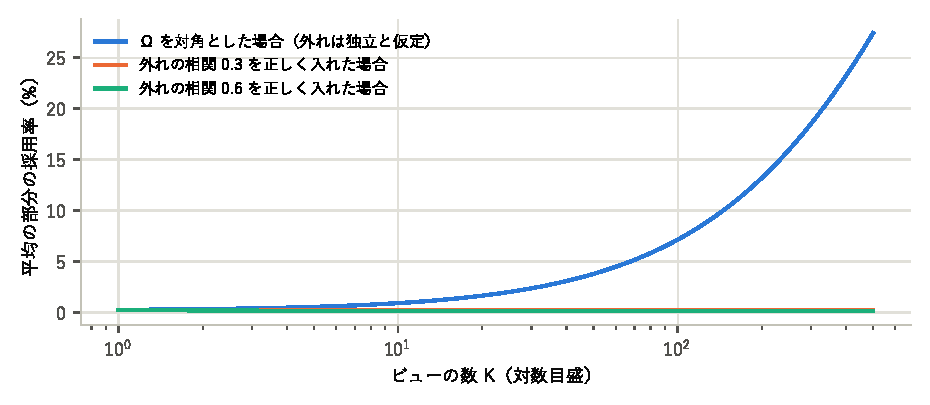
\includegraphics[width=0.92\linewidth]{fig_stack.pdf}
\caption{ビューの数と、平均の方向の採用率。外れが独立と仮定すると（青）、ビューが増えるほど全体の水準を強く信じる。外れの相関を正しく入れると（橙・緑）、採用率は増えない。}
\label{fig:stack}
\end{figure}

\tabref{tab:stack} と\figref{fig:stack} のとおり、外れの相関が 0.3 のとき、正しい採用率は $K$ によらず \V{stk.k500.true}\% だが、対角の $\Omega$ では $K=500$ で \V{stk.k500.diag}\% になる。100 倍以上の積み上がりである。

\section{本プロジェクトの外れの共通部分}

本プロジェクトの LLM の予想の外れ（予想 $-$ 翌月の実際）に、どれくらい共通の部分があるかを測った。判断日ごとの外れの平均の分散と、銘柄ごとの外れの分散の比から、等相関のモデルの $\rho_e$ を推定すると、約 \V{stk.rhoe} だった。外れの分散のうち、月ごとの共通の部分が占める割合は \V{stk.common.share}\% 程度である。

さらに、判断日ごとの予想の平均（LLM が見込む「全体の水準」）と、翌月の実際の平均の相関は \V{stk.level.corr} で、負だった。予想の平均の散らばり（日次 \V{stk.qlevel.sd}\%）は、実際の平均の散らばり（日次 \V{stk.rlevel.sd}\%）と同じくらいの大きさなのに、向きが合っていない。30 か月しかないので確かなことは言えないが、少なくとも「全体の水準の予想を数百倍に積み上げて信じる」根拠は、データにない。

\section{どう防ぐか}

\begin{enumerate}
\item \textbf{$\Omega$ を $\Sigma$ に比例させる}：$\Omega=\tau(1/s-1)P\Sigma P\T$（市場版なら $(1/s-1)P\Sigma P\T$）。外れの相関をリターンの相関と同じとみなす。どの方向にも採用率 $s$ がかかり、積み上がらない。本プロジェクトの計算（\chapref{ch:project}）の「$\Sigma$ に比例」の版である。
\item \textbf{全体の水準と差を分ける}：予想から判断日ごとの平均を引いて相対ビューにし、全体の水準は（入れるなら）別の 1 つのビューとして、それに見合う不確かさで入れる（\chapref{ch:shape}）。本プロジェクトのように全体の水準の予想が当たっていないなら、入れないのがよい。
\item \textbf{外れの共分散を推定する}：過去の外れから、共通の部分（ファクター）と個別の部分を推定し、$\Omega$ を「ファクターの構造」で作る。データが十分にあれば、もっとも正確である。
\end{enumerate}

\begin{keybox}[この章のまとめ]
\begin{itemize}
\item ビューの外れに共通の部分があるのに $\Omega$ を対角にすると、全体の水準への確信がビューの数に比例して積み上がる。例では、500 個のビューで採用率が 0.25\% から \V{stk.k500.diag}\% になった。
\item 外れの相関をリターンの相関と同じにする（$\Omega\propto\Sigma$）と、ビューの数によらず採用率は $\IC^2$ のままになる。
\item 銘柄間の差の予想は、全体の水準の予想より確かである。相対ビューにして、全体の水準は別に扱う。
\item 本プロジェクトの予想の外れの相関は約 \V{stk.rhoe} で、全体の水準の予想は翌月の実際と負の相関（\V{stk.level.corr}）だった。
\end{itemize}
\end{keybox}

% ============================================================
\chapter{ビューの形：絶対・相対・順位・ファクター}\label{ch:shape}

同じ情報でも、ビューの形（行列 $P$）の選び方で、BL の結果は変わる。この章では、ビューの形の選択肢と、それぞれが何を変えるのかを整理する。とくに、LLM の予想のように「全体に楽観的すぎる」「全体に悲観的すぎる」といった癖がある予想では、相対ビューにするだけで、その癖を取り除ける。

\section{絶対ビュー}

1 つの資産の期待リターンを直接言うビューである。$p_k$ は、その資産の位置だけが 1 で、ほかは 0 の行ベクトルになる。対象論文と本プロジェクトは、全銘柄に絶対ビューを置き、$P=I$ としている。

絶対ビューには、銘柄ごとの差の情報と、全体の水準の情報が混ざっている。例えば、全銘柄の予想が一律に 0.1\% 高ければ、それは「市場全体が上がる」というビューである。BL はそれを、すべての銘柄の期待リターンを上げる方向に使い、制約のない最適化なら、市場ポートフォリオを買い増す（合計が 100\% を超える）。全額投資の制約があると、その情報は使い道がなく、ベータの高い銘柄に寄せるなど、意図しない形で比率に出る。

\section{相対ビュー}

2 つ以上の資産の差を言うビューである。$p_k$ の和は 0 で、上回る側に正、下回る側に負の重みを置く。相対ビューは、全体の水準についての情報を含まない。運用者の多くは、「A は B より良い」という形で考えることが多いので、相対ビューのほうが自然だと Idzorek は述べている。

重みの付け方は、\chapref{ch:idzorek} で見たとおり、時価総額の重み（Idzorek）と等しい重み（Satchell and Scowcroft）がある。時価総額の重みのほうが、小さい資産を不必要に大きく動かさずに済む。

\subsection*{LLM の予想を相対ビューにする}

対象論文の第 2 版は、LLM ごとに「投資スタイル」があり、それが成績を決めると結論している。論文の表 4 によると、回答の平均は、Gemma が $-0.38$\%、Qwen が $+0.10$\%、Llama が $+0.18$\%、GPT-4o-mini が $+0.13$\%（いずれも日次）で、Gemma は全体に悲観的だった。論文は、上昇相場では楽観的なモデルが勝ったと述べている。

これは、絶対ビューの「全体の水準」の部分が成績を決めた、ということである。全体の水準の予想は、市場全体の方向を当てる予想で、1 本の予想にすぎない（独立な予想の数が少ない）。それを数百のビューに分けて入れ、$\Omega$ を対角にすると、確信が数百倍に積み上がる（\secref{sec:diag-trap}）。

対策は、ビューから全体の水準を取り除くことである。

\begin{enumerate}
\item \textbf{平均を引く}：各時点で予想の平均（または時価総額加重の平均）を引き、$\tilde Q=Q-\bar Q\one$ を相対ビューとして使う。$P=I-\frac1N\one\one\T$（または時価総額の重みで引く形）になる。
\item \textbf{ペアやグループの差にする}：「上位 10\% の平均は下位 10\% の平均を上回る」のような、少数のロング・ショートのビューにまとめる。
\item \textbf{全体の水準は別の 1 つのビューにする}：市場全体の方向について言いたいことがあれば、市場ポートフォリオについての 1 つのビューとして、それに見合う不確かさで入れる。
\end{enumerate}

1 番目の $P=I-\frac1N\one\one\T$ は階数が $N-1$ で、$P\tau\Sigma P\T$ は逆行列を持たない。$\Omega$ が正定値なら、更新形の $(P\tau\Sigma P\T+\Omega)^{-1}$ は計算できる。

\subsection*{全体の水準が比率に効くのはいつか}

全体の水準の癖がいつ比率を動かすかは、$\Omega$ の形と、最適化の制約で決まる。

\begin{itemize}
\item \textbf{$\Omega\propto\Sigma$ で、全額投資の制約があるとき}：事後の期待リターンは $\Pi+s(Q-\Pi)$ で、$Q$ を一律に $c$ だけ上げると、すべての銘柄の期待リターンが $sc$ だけ一律に上がる。全額投資（比率の和が 1）なら、一律の上乗せは目的関数に定数を足すだけで、比率は変わらない。全体の水準の癖は、自動的に打ち消される（\chapref{ch:project} で確かめた）。
\item \textbf{$\Omega$ が対角のとき}：一律の上乗せ $c\one$ は、事後では $c\,\tau\Sigma(\tau\Sigma+\Omega)^{-1}\one$ になり、銘柄ごとに違う大きさで配られる。市場との共分散が大きい（ベータの高い）銘柄ほど大きく上がる。楽観的な予想は高ベータの銘柄への傾きに、悲観的な予想は低ベータの銘柄への傾きになる。上昇相場で楽観的な LLM が勝った、という対象論文の「スタイル」の結果は、この仕組みで説明できる。
\item \textbf{全額投資の制約がないとき}：全体の水準の上げ下げは、そのまま市場への投資額の増減になる。
\end{itemize}

相対ビューにする（平均を引く）のは、とくに $\Omega$ が対角の場合や、全額投資の制約がない場合に大切である。

\section{ポートフォリオへのビュー}

セクターや国、スタイルなど、資産のまとまりについてのビューである。$p_k$ はそのまとまりの比率（時価総額の重み）になる。「エネルギーのセクターは市場を 2\% 上回る」なら、エネルギー株の時価総額の比率から市場の比率を引いた行になる。

まとまりについてのビューは、個別の銘柄のビューより当たりやすいとは限らないが、個別の雑音が平均で消えるので、外れの分散は小さくなる。また、ビューの数が少ないので、$\Omega$ の相関の扱いも簡単になる。月次レポートのような、セクターや国の単位で書かれた情報は、この形にすると素直に入る（『総合報告書』の「月次レポートの読み取り」の章）。

\section{順位のビュー}

予想の値には自信がないが、順番には意味がある、という場合がある。Almgren と Chriss（2006）は、期待リターンの順序だけが分かっているときの最適なポートフォリオを考え、順序と矛盾しない期待リターンの集合の「中心」を使う方法を示した。Meucci（2010）は、順位のような「緩い」ビューを扱える方法として、Almgren and Chriss とエントロピー・プーリング（\chapref{ch:ep}）を挙げている。

実務でよく使われる簡単な方法は、順位を正規分布の点数に直し、Grinold の式で大きさを決めることである。
\begin{equation}
z_i=\Phi^{-1}\!\left(\frac{\mathrm{rank}_i-0.375}{N+0.25}\right),\qquad
\alpha_i=\IC\cdot\sigma_i\cdot z_i
\end{equation}
$\Phi^{-1}$ は標準正規分布の分位点（Blom の近似）。順位の当たり具合（順位相関の IC）だけで、期待リターンの大きさが決まる。LLM に数値ではなく順位や区分（強気・中立・弱気）を答えさせる場合にも使える。

\section{ファクターへのビュー}

資産の数が多いとき、すべての資産にビューを置くのは大変で、外れの相関の扱いも難しい。ファクター（市場、規模、バリュー、モメンタムなど）についてのビューにすれば、数が少なく、意味も分かりやすい。

\subsection*{ファクターモデルの BL}

資産のリターンがファクターモデル
\begin{equation}
r=Bf+\epsilon,\qquad f\sim\mathcal N(\mu_f,F),\qquad \epsilon\sim\mathcal N(0,D)
\end{equation}
に従うとする。$B$ は露出（$N\times L$）、$\mu_f$ はファクターのリスクプレミアムである。Kolm と Ritter（2017）は、裁定価格理論（APT）の文脈で、$\mu_f$ に事前分布 $\mathcal N(\xi,V)$ を置き、ファクターについてのビュー $P_f\mu_f=Q_f+\varepsilon_f$ で更新する形を詳しく扱っている。Spears ほか（2023）はこれを BL--APT と呼び、階層ベイズのモデルとして書き直した。

ファクターのプレミアムの事後分布は、ふつうの BL と同じ形である。
\begin{align}
\mu_f^{\mathrm{post}}&=\xi+VP_f\T(P_fVP_f\T+\Omega_f)^{-1}(Q_f-P_f\xi)\\
V^{\mathrm{post}}&=V-VP_f\T(P_fVP_f\T+\Omega_f)^{-1}P_fV
\end{align}
資産の期待リターンは $B\mu_f^{\mathrm{post}}$、予測の共分散は $B(F+V^{\mathrm{post}})B\T+D$ になる。Spears ほかは、この予測分布のもとでの最適な比率を、行列の公式を使って閉じた形で書いている。

ファクターへのビューの利点は次のとおりである。

\begin{itemize}
\item ビューの数が少ない（数個〜数十個）。外れの相関も、ファクターの共分散 $F$ を使えば自然に入る。
\item 1 つのビューが、露出 $B$ を通じて全資産に一貫した形で効く。
\item ファクターのプレミアムには長い歴史のデータがあるので、事前分布 $\xi$、$V$ と、ビューの当たり具合を測りやすい。
\end{itemize}

数値例は \chapref{ch:esg} で、セクター ETF と Fama--French のファクターを使って示す。

\subsection*{ほかの拡張}

Meucci（2009）は、資産のリターンではなく、一般的なリスクファクター（金利、ボラティリティなど、損益に非線形に効くもの）にビューを置き、ストレステストにも使える形に拡張した。Cheung（2013）の Augmented BL は、ファクターへのビューを中心にした BL で、ファクターのランキングに頼らずに、ファクターに基づくポートフォリオを作る方法を示している。

\section{外部の変数へのビュー}

ビューを置く対象は、投資する資産でなくてもよい。Meucci（2010）は、マクロ経済の変数のような「外部の要因」についてのビューを、相関を通じて資産のリターンに反映させる使い方を、BL では扱えず COP やエントロピー・プーリングなら扱える例として挙げている。実は、市場版の BL でも、外部の変数 $g$ を資産のリターン $X$ と一緒に並べた $(X,g)$ の正規分布を考えれば、$g$ へのビューで $X$ を条件付けられる。

\begin{equation}
\E[X\mid g=v]=\pi_X+\Sigma_{Xg}\,\Sigma_{gg}^{-1}(v-\pi_g)
\end{equation}
これは、$g$ への回帰の係数で $X$ を動かすことと同じである。\chapref{ch:politics} で、地政学リスク指数の変化を外部の変数にした例を示す。

\section{ビューの数と、ビューどうしの関係}

\begin{itemize}
\item \textbf{ビューの数}：$K\le N$ である必要はないが、$K$ が多いほど、外れの相関の扱いが重要になる。
\item \textbf{同じことを言うビュー}：例えば「A は 5\%」「B は 3\%」「A$-$B は 2\%」の 3 つは、3 つ目が前の 2 つから決まる。外れが独立だと扱うと、同じ情報を 2 回数えることになる。
\item \textbf{矛盾するビュー}：「A$-$B は 2\%」「A$-$B は $-1\%$」のように食い違うビューは、不確かさに応じた平均になる。食い違いが大きいなら、どちらかの不確かさを見直す（\chapref{ch:text} の融合の方法）。
\item \textbf{計算の安定性}：$P\Sigma P\T$ がほぼ特異（ビューのポートフォリオがほとんど同じ）だと、100\% に近い確信で計算が不安定になる。
\end{itemize}

\begin{tipbox}[コツ：ビューの形]
\begin{enumerate}
\item 全体の水準と銘柄間の差は、別々に考える。銘柄間の差は相対ビュー（平均を引く）、全体の水準は市場への 1 つのビューにする。
\item 相対ビューの重みは時価総額で付ける。
\item 予想の値に自信がないときは、順位を点数に直し、IC で大きさを決める。
\item 資産が多いときは、ファクターへのビューを検討する。数が少なく、相関も自然に入る。
\item 同じ情報を 2 回数えていないか、ビューを並べて確かめる。
\end{enumerate}
\end{tipbox}

\begin{keybox}[この章のまとめ]
\begin{itemize}
\item 絶対ビューは、銘柄間の差と全体の水準を混ぜて持つ。LLM の「スタイル」（全体の楽観・悲観）は、この全体の水準の部分である。
\item 相対ビュー（平均を引く、ペアにする）にすれば、全体の水準の癖を取り除ける。
\item ファクターへのビューは、数が少なく、相関が自然に入り、データで当たり具合を測りやすい。
\item 外部の変数へのビューも、資産と一緒の正規分布を考えれば、市場版の BL で扱える。
\end{itemize}
\end{keybox}


\part{ファクターごとの数値化}
% ============================================================
\chapter{政治と政策の不確かさ}\label{ch:politics}

戦争やテロ、選挙、関税、規制の変更は、株価を大きく動かす。調査メモは、地政学リスク指数（GPR）や経済政策不確実性指数（EPU）を使って、こうした政治のファクターを BL のビューと不確かさに変換する方法を論じている。この章では、まず指数の作り方を論文に沿って確かめ、次に BL への入れ方を 3 通りに分けて、それぞれを本プロジェクトのデータ（2015〜2026 年）で試す。

\section{地政学リスク指数（GPR）}

\begin{paperbox}[Caldara and Iacoviello（2022）, \textit{Measuring Geopolitical Risk}, American Economic Review 112(4)]
\begin{itemize}
\item \textbf{作り方}：新聞の記事のうち、悪い地政学的な出来事に触れた記事の割合を、月ごとに数える。最近の指数（1985 年から）は、アメリカ・イギリス・カナダの 10 紙（Chicago Tribune、Daily Telegraph、Financial Times、Globe and Mail、Guardian、Los Angeles Times、New York Times、USA Today、Wall Street Journal、Washington Post）の電子版を検索する。1900 年からの長い指数は、3 紙の紙面の記録を使う。
\item \textbf{検索の 8 区分}：戦争の脅威、平和への脅威、軍備の増強、核の脅威、テロの脅威（ここまで「脅威」）と、戦争の開始、戦争の激化、テロの実行（「行動」）。1 語だけの検索は誤りが多いので、2 つの語の組み合わせや、近くに現れる語で検索する。
\item \textbf{分解}：「脅威」の区分から GPRT、「行動」の区分から GPRA を作れる。
\item \textbf{確かめ方}：人が記事を読んで作った物語の記録や、さまざまな頑健性の確認で、自動の指数が意味のある動きをしていることを示す。
\item \textbf{結果}：1985〜2019 年のデータで、地政学リスクのショックは、投資と雇用の長く続く低下をもたらす。悪影響は、脅威と実際の出来事の両方から来る。
\end{itemize}
\end{paperbox}

指数は 2021 年 10 月に改訂され、検索の語が少し変わり、最近の指数は 1985〜2019 年の平均が 100 になるようにそろえられている。この資料で使ったデータ（\V{unc.start}〜\V{unc.end}）では、GPR の中央値は \V{unc.gpr.med}、最大は \V{unc.gpr.argmax} の \V{unc.gpr.max} だった。

\section{経済政策不確実性指数（EPU）}

\begin{paperbox}[Baker, Bloom and Davis（2016）, \textit{Measuring Economic Policy Uncertainty}, Quarterly Journal of Economics 131(4)]
\begin{itemize}
\item \textbf{作り方}：アメリカの主要な 10 紙（USA Today、Miami Herald、Chicago Tribune など）で、「経済」の語、「政策」の語（議会、財政赤字、連邦準備制度、立法、規制、ホワイトハウスなど）、「不確実」の語の 3 つをすべて含む記事の数を、月ごとに数える。新聞ごとに記事の総数で割り、標準化して平均し、1985〜2009 年の平均が 100 になるようにそろえる。
\item \textbf{確かめ方}：12,000 本の記事を人が読む監査を行い、自動の分類と比べた。政策の語の選び方も、この監査の結果で決めた。
\item \textbf{長い歴史}：6 紙の記録で 1900 年までさかのぼる。1931 年の終わりから大きく上がり、1960 年代から上がり続けている。
\item \textbf{結果}：接戦の大統領選挙、湾岸戦争、9.11、リーマン・ブラザーズの破綻、2011 年の債務上限の争いなどで急上昇する。企業の単位では、政策の不確実性は株価の変動を大きくし、政策に敏感な業種（防衛、医療、インフラ）の投資と雇用を減らす。
\end{itemize}
\end{paperbox}

この資料のデータでは、EPU の中央値は \V{unc.epu.med}、最大は \V{unc.epu.argmax} の \V{unc.epu.max} だった。\figref{fig:unc-series} に、EPU と GPR の内訳の推移を示す。

\begin{figure}[htbp]
\centering
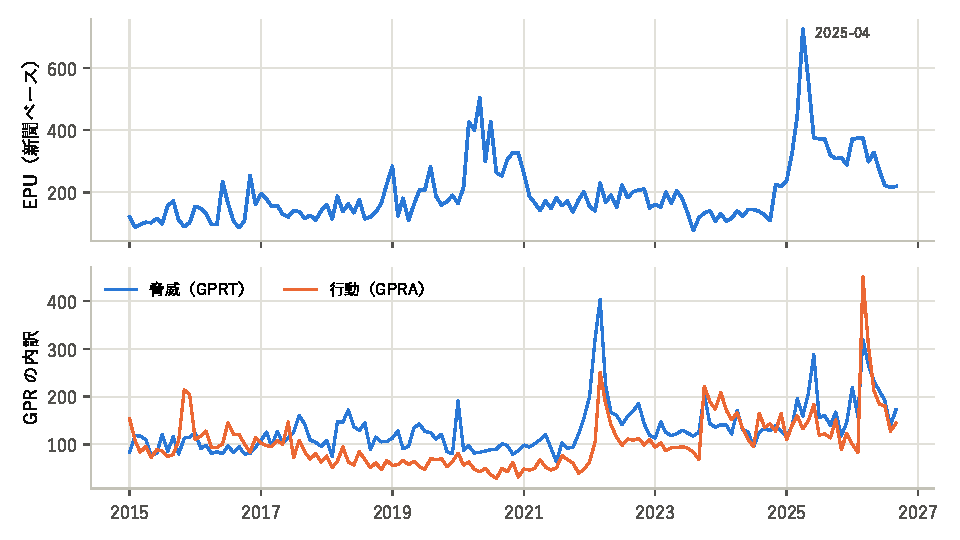
\includegraphics[width=0.95\linewidth]{fig_unc_series.pdf}
\caption{経済政策不確実性指数（上）と、地政学リスク指数の内訳（下：脅威 GPRT と行動 GPRA）。月次、\V{unc.start}〜\V{unc.end}。}
\label{fig:unc-series}
\end{figure}

\section{企業ごとの政治リスク}

\begin{paperbox}[Hassan, Hollander, van Lent and Tahoun（2019）, \textit{Firm-Level Political Risk: Measurement and Effects}, Quarterly Journal of Economics 134(4)]
\begin{itemize}
\item \textbf{作り方}：上場企業の四半期の決算説明会の書き起こしで、政治に関する話題にどれだけの時間が割かれ、それがリスクや不確実性と結びついているかを数える。政治の文章（教科書、新聞の政治面、政治の演説など）とそれ以外の文章を比べて、政治の文章に特に多い 2 語の組み合わせ（bigram）を選び、それがリスクを表す語の近くに現れる回数を数える。
\item \textbf{データ}：この資料で確かめた NBER の版では、2002〜2016 年に、アメリカで上場する 9,478 社が行った 175,797 回の決算説明会である。
\item \textbf{結果}：政治リスクの大部分は、業種や時期では説明できない企業ごとのもので、ばらつきが大きい。政治リスクが高い企業は、投資と採用を減らし、ロビー活動や献金を増やす。
\end{itemize}
\end{paperbox}

調査メモは、この方法を応用した分析として「約 7,000 社の 24 万件を超える決算説明会」から企業ごとの地政学リスクのセンチメントを取り出し、航空・運輸が悪影響を受け、防衛が恩恵を受けることを捉えた、と書いている。この資料では、その数字と結果を述べた論文を確認できなかった（\appref{app:check}）。企業ごとの政治リスクの測り方としては、上の論文が出発点になる。

\section{政治リスクは期待リターンに効くか}

政治の不確かさが、期待リターン（リスクプレミアム）とボラティリティの両方に効くことは、理論と実証の両方で論じられている。

\begin{itemize}
\item Pástor と Veronesi（2012、2013）は、政府の政策の不確かさが株価にリスクプレミアムを要求させ、ボラティリティと銘柄間の相関を高めることを、理論のモデルで示した。
\item Brogaard と Detzel（2015）は、EPU が資産価格に織り込まれたリスクの要因であることを実証し、EPU の上昇が同時点のリターンの低下と、その後のリターンの上昇（リスクプレミアム）に結びつくことを報告している。
\end{itemize}

BL の言葉に直すと、政治の不確かさが高まったときには、(1) 期待リターンの見込み（$Q$）が変わりうる、(2) リターンの散らばり（$\Sigma$）が大きくなる、(3) 予想の外れ（$\Omega$）も大きくなる、の 3 つが起きうる。以下、それぞれを順に見る。

\section{入れ方 1：感応度からビューを作る}

調査メモは、資産のリターンと GPR・EPU の時系列モデル（VAR など）を作り、ショックへの反応（インパルス応答）を測って、それをビュー $Q$ にする方法を挙げている。もっとも簡単な形は、市場のリターンを入れたうえで、指数の変化への感応度を回帰で測ることである。
\begin{equation}
r_{s,t}-r_{f,t}=a_s+\beta_{s}^{\mathrm{mkt}}(r_{m,t}-r_{f,t})+\beta_s^{\mathrm{EPU}}\Delta\log\mathrm{EPU}_t+\beta_s^{\mathrm{GPR}}\Delta\log\mathrm{GPR}_t+e_{s,t}
\end{equation}
セクター ETF の月次リターンで推定した結果を\tabref{tab:unc-sector}に示す。

\begin{table}[htbp]
\centering
\caption{セクター ETF の月次超過リターンの、EPU・GPR の変化への感応度（2015〜2026 年）。「+10\%」の列は、指数が 10\% 上がった月のリターンの違い（\%）。$t$ 値は White の標準誤差による。}
\label{tab:unc-sector}
\tabin{unc_sector}
\end{table}

感応度の $t$ 値は、ほとんどが 2 を下回る。公益は EPU と GPR の上昇月にやや強く、金融とエネルギーは EPU の上昇月にやや弱いが、偶然と区別できる大きさではない。月次で 10 年分のデータでは、セクターの政治の感応度ははっきり測れない。

仮に感応度が測れたとしても、ビューにするには「来月、指数がどう動くか」の予想が必要になる。指数の変化を予想するのは、株価を予想するのと同じくらい難しい。感応度からビューを作る方法は、次の「シナリオ」の形で使うほうが素直である。

\section{入れ方 2：シナリオとして入れる}

「もし地政学リスクが 50\% 高まったら」というシナリオを、外部の変数へのビューとして入れる（\chapref{ch:shape}）。セクターの超過リターンと指数の変化を並べた変数 $(X,g)$ の共分散を、全セクターの ETF がそろう 2018 年 7 月からの \V{scen.n} か月で推定し、市場版の BL で $g=\log1.5$（50\% の上昇）という条件を付ける。均衡のずれは 0 とした。

\begin{table}[htbp]
\centering
\caption{指数の 50\% 上昇を外部の変数へのビューとして入れたときの、セクターの期待リターンの変化（月次 \%）。「確実」は $\Omega\to0$（シナリオ分析）、「$c=1$」は $\Omega$ を指数の変化の分散と同じにしたもの。指数の月次の変化の標準偏差は、GPR が \V{scen.dgpr.sd}\%、EPU が \V{scen.depu.sd}\%。}
\label{tab:unc-scen}
\tabin{unc_scen}
\end{table}

\tabref{tab:unc-scen} のとおり、GPR が 50\% 上がるシナリオでは、公益を除く全セクターが月次で 0.5〜2\% 下がる。EPU のシナリオでは、エネルギー、金融、資本財が大きく下がり、ヘルスケアと公益はほとんど動かない。

ただし、この数字は「過去 8 年あまりの相関がこれからも続くなら」という条件付きである。GPR の変化とセクターのリターンの相関は $-0.24$〜0 と小さく、推定の誤差も大きい。シナリオの結果は、確実（$\Omega\to0$）で入れるより、$c=1$ のように控えめに入れ、ストレステストとして比率の変化を確かめる使い方が向いている。Meucci が BL の市場版を「シナリオ分析」と結びつけたのは、この使い方である。

\section{入れ方 3：不確かさ $\Omega$ を伸び縮みさせる}

調査メモがもっとも強調しているのは、政治の不確かさが高い時期に $\Omega$ を大きくして、ビューの確信度を自動的に下げる、という使い方である。

\begin{paperbox}[Han and Li（2023）, \textit{The impact of global economic policy uncertainty on portfolio optimization: A Black--Litterman approach}, International Review of Financial Analysis 86]
\begin{itemize}
\item 世界の経済政策不確実性（GEPU）が、世界の資産配分に非対称に効くことを調べる。
\item 二重に非対称な GARCH-MIDAS（DAGM）のモデルで、GEPU のショックが、世界の株式、債券、商品、クリーンエネルギー、ビットコインの長期のボラティリティに与える影響を推定する。
\item GEPU に基づくボラティリティを、BL の投資家のビューの不確かさとして使う。
\item 標本外の検証で、GEPU に基づくモデルは、多くの場合に従来の基準よりリスク調整後のリターンが高かった。
\end{itemize}
\end{paperbox}

この方法が働くには、「政治の不確かさが高い時期には、予想が外れやすい（ボラティリティが高い）」ことが必要である。本プロジェクトのデータで、月末の指数の水準が、翌月の \SP{} の実現ボラティリティ（日次リターンの標準偏差の年率）を予想できるかを調べた。

\begin{table}[htbp]
\centering
\caption{翌月の \SP{} の実現ボラティリティ（対数）の回帰（\V{unc.reg.n} か月）。説明変数は、当月の実現ボラティリティ、EPU、GPR の対数。}
\label{tab:unc-reg}
\tabin{unc_reg}
\end{table}

結果は次のとおりである。

\begin{itemize}
\item 単独の相関では、EPU は翌月のボラティリティと \V{unc.cor.epu}、GPR は \V{unc.cor.gpr} の相関を持つ。当月の実現ボラティリティは \V{unc.cor.rv}、VIX は \V{unc.cor.vix} である。
\item 当月の実現ボラティリティを入れると、EPU の $t$ 値は \V{unc.reg.epu.t}、GPR は \V{unc.reg.gpr.t} で、追加の説明力はない（\tabref{tab:unc-reg}）。
\item VIX を入れると、VIX の $t$ 値は \V{unc.reg2.vix.t} で強く、EPU は \V{unc.reg2.epu.t} とむしろ負になった。
\end{itemize}

少なくとも、翌月という短い期間では、政治の指数は市場のボラティリティ（直近の実現値や VIX）にない情報をほとんど持っていない。新聞の記事の数より、市場の価格のほうが早く、正確に不確かさを映しているためと考えられる。Han と Li の方法が長期のボラティリティの成分（MIDAS）を使っているのは、政策の不確かさが効くのは月次より長い期間だ、という見方と整合する。

それでも EPU で $\Omega$ を伸び縮みさせたらどうなるかを、\chapref{ch:macro} の\figref{fig:adoption-time}に示した。EPU の中央値で採用率 50\% になるように置くと、関税をめぐる不確実性が急上昇した 2025 年 4 月には、採用率は \V{epu.adopt.min}\% まで下がる。仕組みとしては働くが、上のとおり、その時期に予想が本当に外れやすいかの裏付けは弱い。

\section{調査メモの記述について}

調査メモは、GPR の「脅威」（GPRT）を不確かさ $\Omega$ を大きくする合図に、「行動」（GPRA）を防衛・エネルギーなどのセクターへの方向のビューに使う、という表を示している。この対応は、Caldara と Iacoviello の論文にはない。論文が示しているのは、脅威と行動の両方が実体経済に悪影響を与えることである。表は、調査メモの提案として読むのがよい。この資料のデータでは、脅威と行動の区別に入る前に、指数そのものが翌月のボラティリティやセクターの差をほとんど説明しなかった。

\begin{tipbox}[コツ：政治のファクターを使うとき]
\begin{enumerate}
\item 感応度を推定して来月のビューにするのは難しい。指数の変化そのものを予想しなければならないうえ、感応度の推定の誤差も大きい。
\item 「もし地政学リスクが高まったら」という問いには、市場版の BL のシナリオ（外部の変数へのビュー）で答える。結果はストレステストとして使い、確実なビューとして入れない。
\item $\Omega$ を伸び縮みさせるなら、まず市場のボラティリティ（直近の実現値、VIX）を使う。政治の指数は、それに加えて説明力があるかを確かめてから使う。
\item 政策の不確かさが効くのは、月次より長い期間かもしれない。期間の長いビューや、長期のボラティリティの成分と組み合わせる。
\end{enumerate}
\end{tipbox}

\begin{keybox}[この章のまとめ]
\begin{itemize}
\item GPR と EPU は、新聞の記事の割合から作る月次の指数である。企業ごとの政治リスクは、決算説明会の書き起こしから測れる（Hassan ほか 2019）。
\item 本プロジェクトのデータ（2015〜2026 年）では、セクターの感応度ははっきりせず、指数は翌月のボラティリティを市場の指標以上には説明しなかった。
\item 政治のファクターは、シナリオ分析と、長い期間の不確かさの見込みに使うのが向いている。
\end{itemize}
\end{keybox}

% ============================================================
\chapter{テキストのセンチメントと LLM}\label{ch:text}

ニュース、掲示板、決算説明会の文章からビューを作る研究は、BERT のような言語モデルの登場で増え、最近は大規模言語モデル（LLM）に直接リターンを予想させる研究も出てきた。本プロジェクトもその 1 つを再現している。この章では、代表的な研究を、ビュー $Q$ と不確かさ $\Omega$ をどう作っているかに注目して読み、そのうえで、LLM の回答のばらつきを $\Omega$ に使うことの是非を考える。

\section{テキストからビューを作る流れ}

どの研究も、おおむね次の流れである。

\begin{enumerate}
\item 文章を集め、銘柄と日付に結びつける。
\item 文章を数値にする（辞書で数える、BERT で分類する、LLM に聞く）。
\item 数値を予想リターンに直す（回帰、LSTM などの予測モデル、価格のシミュレーション、LLM の回答そのもの）。
\item 予想をビュー $Q$ にし、不確かさ $\Omega$ を決める。
\end{enumerate}

研究によって工夫があるのは 2 と 3 で、4 の $\Omega$ は簡単に済ませているものが多い。ところが、BL の結果を大きく決めるのは 4 である（\chapref{ch:overview}）。

\section{BERT のセンチメントをビューにした研究}

\begin{paperbox}[Colasanto, Grilli, Santoro and Villani（2022）, \textit{BERT's sentiment score for portfolio optimization: a fine-tuned view in Black and Litterman model}, Neural Computing and Applications 34]
\begin{itemize}
\item Financial Times の記事のセンチメントの極性の点数を、BL の新しいビューとして使う。
\item 記事が出たあとの数取引時間の価格の経路をモンテカルロ法でシミュレーションし、得られた価格を利回りに直して、時間ごとの価格に基づく「動的な」最適化のビューにする。
\item センチメントを使わないビュー（初めのポートフォリオを変えない）と比べる。
\end{itemize}
本文は確認できず、要旨の範囲で記した。
\end{paperbox}

\begin{paperbox}[Sun, Fu and Liu（2026）, \textit{Investor sentiment and stock portfolio construction: A study based on the Black-Litterman model}, PLOS ONE 21(9)]
\begin{itemize}
\item \textbf{データ}：上海 50 指数の 8 銘柄（保利発展、中国聯通、恒瑞医薬、伊利、中国建築、中国銀行、中国石化、中微公司）について、投資家の掲示板（東方財富の股吧）の書き込みを 2022 年 7 月〜2024 年 12 月に集め、自動投稿や重複を除いて 387,953 件。
\item \textbf{センチメント}：辞書の方法と、中国語 BERT を 3 区分（悪い・中立・良い）に微調整した方法。閲覧数と返信数で重み付けして、銘柄ごとの日次の指数にする。BERT の正解率は、学習に使った領域の検証データで 74.69\%、掲示板の書き込み 1,000 件を人が付けた正解と比べると 52.3\% だった。
\item \textbf{予想}：始値・高値・安値・終値・出来高とセンチメントを LSTM に入れ、対数リターンを予想する。2022 年 7 月〜2024 年 7 月で学習、2024 年 7 月 11 日〜12 月 31 日で検証。
\item \textbf{BL}：LSTM の予想を絶対ビュー $Q$ にし、ビューの不確かさは $8\times8$ の単位行列と書かれている。事前の共分散は過去 200 取引日。毎日見直し、117 取引日で評価。
\item \textbf{結果}：取引費用なしで、BERT のビューの BL は年率 106.58\%、シャープレシオ 2.64、ソルティノレシオ 4.18。辞書とセンチメントなしの BL より良く、取引費用を入れても最も高い年率リターンを保った。
\item \textbf{限界}（著者による）：書き込みは個人投資家が中心、文章の雑音、汎用の BERT の限界、滑りや比率の上限を入れていない、8 銘柄・1 期間だけ。
\end{itemize}
\end{paperbox}

調査メモは、この論文の年率 106.58\%、シャープレシオ 2.64、ソルティノレシオ 4.18 を「極めて優れた」成績として紹介している。数字は論文どおりだが、次の条件を添えて読む必要がある。

\begin{itemize}
\item 評価期間は 117 取引日（約 5 か月半）で、その終わりの 2024 年秋は中国株が大きく上がった時期である。年率に直した 106\% は、5 か月余りの上昇を 1 年に引き延ばした数字である。
\item 銘柄は 8 つだけで、どの銘柄を選ぶかで結果が大きく変わりうる。
\item ビューの不確かさが単位行列だとすると、日次の対数リターン（$10^{-4}$ 程度の分散）に対して $\Omega$ の対角が 1 なので、ビューはほとんど採用されないはずである。単位が違う（パーセントで書いている、など）のか、別の扱いをしているのか、本文の範囲では確認できなかった。$\Omega$ の大きさは結果を左右するので、再現するならここを最初に確かめる必要がある。
\item センチメントの分類器の正解率は、実際の書き込みでは 52.3\%（3 区分でのでたらめは 33\%）だった。
\end{itemize}

\begin{paperbox}[Mantshimuli and Muteba Mwamba（2025）, \textit{Enhancing portfolio optimization with multi-LLM sentiment aggregation: A Black-Litterman integration approach}, Investment Management and Financial Innovations 22(3)]
\begin{itemize}
\item 金融向けに微調整した 3 つの LLM のセンチメントの点数を、LSTM で 1 つの「メタ LLM」の点数にまとめ、BL の投資家のビューにする。
\item \SP{} の銘柄で検証し、年率 31.22\%（時価総額加重は 24.57\%）、シャープレシオ 3.02、オメガレシオ 2.48、ジェンセンのアルファ 1.95\% と報告している。単一の LLM のポートフォリオより良かった。
\item 要旨の範囲では、検証期間や取引費用は分からなかった。
\end{itemize}
\end{paperbox}

\section{対象論文：LLM の予想と回答のばらつき}

\begin{paperbox}[Lee, Kim, Kim, Kim and Lee（2025）, \textit{LLM-Enhanced Black-Litterman Portfolio Optimization}, CIKM 2025 FinAI ワークショップ（arXiv 2504.14345 第 2 版）]
\begin{itemize}
\item \textbf{データ}：2025 年 3 月 26 日時点の \SP{} の時価総額上位 50 銘柄。2024 年 6 月〜2025 年 6 月の 13 か月を、検証用 3 か月と評価用 10 か月に分ける。2 週間ごとに見直す。
\item \textbf{LLM}：Gemma-7B、Qwen-2-7B、LLaMA-3.1-8B、GPT-4o-mini。いずれも学習データの締め切りが評価期間より前。
\item \textbf{質問}：過去 2 週間の日次リターン、セクターと \SP{} の日次リターン、会社の情報を渡し、次の 2 週間の日次の平均リターンを 1 つの数で答えさせる。
\item \textbf{ビュー}：各銘柄について 100 回聞き、回答の平均を $Q$、回答の分散を $\Omega$ の対角にする。$P=I$（全銘柄に絶対ビュー）。
\item \textbf{$\tau$}：検証期間で、平均($\Omega$) ÷ 平均($\Sigma$) を中心に 0.5〜1.5 倍の 5 点を試し、シャープレシオで選ぶ。最適化は $w\T\Sigma w-\lambda w\T r$（$\lambda=0.1$）を、全額投資・空売りなしで最小化。取引費用は比率の変化の 0.1\%。
\item \textbf{結果}：年率の成長率は Qwen 28.11\%、Llama 27.51\%、Gemma 15.90\%、GPT 7.68\%、等金額 19.07\%、平均分散 6.07\%。年率のシャープレシオは Llama 1.23、Qwen 1.06。
\item \textbf{解釈}：LLM ごとに一貫した「投資スタイル」（Gemma は悲観、Qwen は控えめな楽観、Llama は大きく散らばる強い確信）があり、成績はそのスタイルと相場の向きが合うかで決まる。
\end{itemize}
\end{paperbox}

本プロジェクトは、この論文の第 1 版（30 回、1 か月の予想）を、全銘柄・30 か月に広げて再現した（『総合報告書』）。調査メモが紹介している「100 回の反復」は第 2 版の設定である。

論文は、回答の分散を $\Omega$ にすることで「確信度が自動で較正される」と述べている。調査メモはさらに進んで、「LLM の出力の統計的なばらつきが、市場の政治的・定性的な情報の不確かさを直接表している」「人が恣意的に決めていた確信度を、テキストデータの内在的なエントロピーから客観的に導出できる」と評価している。次の節で、この主張を検討する。

\section{回答のばらつきは何を測っているか}

同じ質問を何度も聞いたときの回答の散らばりは、LLM が次の語を確率的に選ぶ仕組み（温度 temperature によるサンプリング）から生まれる。散らばりの大きさは、次のようなもので決まる。

\begin{itemize}
\item \textbf{温度の設定}：温度を 0 に近づければ、回答はほとんど同じになる。本プロジェクトは温度 1.0 で聞いている。温度を変えれば $\Omega$ が変わり、BL の結果が変わる。
\item \textbf{質問の書き方}：出力の形式（数値だけ、桁数）や、渡す数値の単位で、散らばり方が変わる。対象論文の第 2 版は、リターンを 100 倍（パーセント）にして渡している。
\item \textbf{入力の値の散らばり}：本プロジェクトでは、回答の散らばりは、渡した月の値動きの大きさと順位相関 0.73 で連動していた（『総合報告書』問題 3）。値動きが大きい銘柄ほど、回答もばらつく。
\end{itemize}

どれも「予想がどれだけ当たるか」とは別のものである。LLM の確信の表明が実際の正しさと合わないことは、言語モデルの研究でも繰り返し報告されている。例えば Xiong ほか（2024）は、LLM に自分の確信度を言わせると、多くの場合に自信過剰になることを示した。Kadavath ほか（2022）は、選択式の問題では大きなモデルの確率がおおむね較正されていることを示したが、それは答えが決まっている問題の話で、来月の株価のように誰にも分からないものの予想とは事情が違う。

本プロジェクトのデータでは、回答の分散と、実際の予想の外れ（誤差の 2 乗）の比は、銘柄・月ごとの中央値で \V{llm.ratio.med}（四分位で \V{llm.ratio.q25}〜\V{llm.ratio.q75}）だった（\chapref{ch:project}）。回答の散らばりは実際の外れの約 8 分の 1 で、BL はその分だけ予想を信じすぎる。

\begin{notebox}[回答のばらつきの使い方]
回答のばらつきが、外れやすさの「順番」の手がかりになる可能性は残る（ばらつく銘柄ほど外れやすい、など）。しかし大きさは合っていない。使うなら、ばらつきの順番だけを使い、大きさは当たり具合で較正する。例えば、$\omega_i=k\cdot(\text{回答の分散}_i)$ として、倍率 $k$ を過去の予想の外れから決める（\chapref{ch:accuracy}）。
\end{notebox}

\section{確率の分布からビューを作る}

LLM に数値を直接答えさせる代わりに、「強気・中立・弱気」の確率を答えさせる方法もある。Florencio（2026）は、論理の述語を確率で表す「neural predicate」の考え方で、この確率から BL の $P$、$q$、$\Omega$ を作る理論の枠組みを提案している。

\begin{itemize}
\item \textbf{ビューの値}：強気の確率を $p_b$、弱気を $p_r$、中立を $p_n$ とし、強気・弱気のときのリターンを $r_{\mathrm{bull}}$、$r_{\mathrm{bear}}$ とする。$q_i=p_b\,r_{\mathrm{bull}}+p_r\,r_{\mathrm{bear}}+p_n\,\Pi_i$（中立なら均衡のまま）。
\item \textbf{不確かさ}：確率の分布のエントロピー $H$ を使う。$\omega_i=\omega_{\min}+(\omega_{\max}-\omega_{\min})\,H/\log3$。分布が 1 つの区分に集中していれば（$H=0$）$\omega_{\min}$、3 区分に均等なら（$H=\log3$）$\omega_{\max}$。$\omega_{\min}$、$\omega_{\max}$ は $\tau\Sigma_{ii}$ の倍数にして、事前の不確かさと単位をそろえる。
\item \textbf{複数の述語の組み合わせ}：述語ごとの $(q,\omega)$ を精度（$1/\omega$）で加重平均し、述語どうしの食い違い（$q$ の分散）が大きいほど $\omega$ を大きくする。
\end{itemize}

\begin{table}[htbp]
\centering
\caption{確率の分布からビューを作る例（月次 \%）。$r_{\mathrm{bull}}=2\%$、$r_{\mathrm{bear}}=-2\%$、$\Pi_i=0.6\%$、$\sigma_i=8\%$、$\tau=0.05$、$\omega/\tau\sigma^2$ を 1〜20 の範囲でエントロピーに比例させた（倍率はこの資料が例として置いたもの）。}
\label{tab:stance}
\tabin{stance}
\end{table}

\tabref{tab:stance} のとおり、確率が強気に集中した銘柄 A は、エントロピーが小さく採用率が高い。3 区分に均等な銘柄 D は、ビューの値も均衡に近く、採用率も低い。仕組みとしては分かりやすい。

ただし、ここでもエントロピーは「LLM がどれだけ迷っているか」であって、「当たり具合」ではない。$\omega_{\min}$、$\omega_{\max}$ をどう置くかで採用率は自由に変わるので、結局は過去の当たり具合で決める必要がある。LLM の確率そのものが較正されているかも確かめる必要がある。本プロジェクトの実験 G（リスクプレミアムの有無の確率を聞く）では、確率の読み取りは使えるが、なめらかではなかった（『総合報告書』）。

\section{複数のモデルの予想をまとめる}

LLM を複数使えば、同じ銘柄について複数のビューが得られる。Spears、Zohren、Roberts（2023）は、同じ資産への複数のビュー（とその不確かさ）をまとめる「融合」の方法を、BL の文脈で整理した。

\begin{description}[leftmargin=2em,style=nextline]
\item[精度加重（PW）] 外れが独立なら、分散の逆数で重み付けして平均するのが最適。まとめた分散は $(\sum_s\hat\Sigma_s^{-1})^{-1}$ で、情報源の数だけ小さくなる。
\item[共分散の交差（CI）] 外れの相関が分からないとき、逆行列の凸結合 $\hat\Sigma^{-1}=\sum_s\omega_s\hat\Sigma_s^{-1}$（$\sum\omega_s=1$）を使う。相関がどうであっても、不確かさを小さく見積もりすぎない（一貫性がある）が、慎重すぎることがある。
\item[逆の共分散の交差（ICI）] CI より慎重さを抑えつつ一貫性を保つ方法。2 つずつまとめる。
\item[共分散の和集合（CU）] どれかの情報源が誤っている（不確かさを小さく言っている）可能性があるときに使う。まとめた分散が、各情報源の分散に平均のずれを足したものを含むようにする。
\end{description}

彼らは、ARIMA、ブースティング、ガウス過程の 3 つのモデルのビューを、BL--APT（\chapref{ch:shape}）で 1992〜2022 年の米国株に当てはめた。年ごとのシャープレシオの中央値は、融合の方法で PW 0.11、CU 0.16、CI 0.38、ICI 0.48 と並び、相関を考える方法のほうが良かった（ただし \SP{} を持ち続けるほうが全体として優れていた）。

\subsection*{外れの相関が大事}

対象論文の表 5 には、4 つの LLM の予想の誤差の 2 乗の平均（MSE）が載っている。これで精度加重の重みを計算すると\tabref{tab:fusion-w}のようになる。

\begin{table}[htbp]
\centering
\caption{対象論文の表 5 の MSE と、精度加重（$1/\mathrm{MSE}$ に比例）の重み。}
\label{tab:fusion-w}
\tabin{fusion_w}
\end{table}

外れが独立なら、まとめた MSE は \V{fu.pw.indep} になり、いちばん良い Qwen（\V{fu.best}）の 3 分の 1 以下になる。しかし、4 つの予想の外れは独立ではない。同じ過去のデータを見て予想し、同じ実現値と比べているので、実現値の側の予想できない動きは、4 つの外れに共通に入る。

\begin{table}[htbp]
\centering
\caption{外れの相関 $\rho$（すべての組で同じとした）を変えたときの、まとめた MSE。「最適な組み合わせ」は、相関を知っていて、重みの和が 1 の範囲で MSE を最小にしたもの（負の重みも許す）。}
\label{tab:fusion-rho}
\tabin{fusion_rho}
\end{table}

\tabref{tab:fusion-rho} のとおり、相関が 0.8 を超えると、精度加重でまとめた MSE は、いちばん良い単独の予想より悪くなる。相関を知っていれば改善の余地はあるが、そのときの重みは大きな正と負の組み合わせになり、相関の推定の誤差に敏感になる。複数の LLM をまとめるときは、独立を仮定した精度加重を避け、CI のような慎重な方法を使うか、それぞれの予想の過去の当たり具合で重みを決める（相関も過去の外れから測る）のがよい。

\begin{tipbox}[コツ：テキストや LLM からビューを作るとき]
\begin{enumerate}
\item 論文の成績は、評価期間の長さ、銘柄の数、取引費用、$\Omega$ の大きさを確かめてから読む。
\item LLM の回答のばらつきやエントロピーは、外れやすさの順番の手がかりにはなりうるが、大きさは当たり具合で較正する。
\item LLM の「スタイル」（全体の楽観・悲観）は相対ビューで取り除き、銘柄間の差だけを使う（\chapref{ch:shape}）。
\item 複数の LLM をまとめるときは、外れの相関を考える。独立を仮定した精度加重は確信を過大にする。
\item 温度や質問の書き方を変えたら、ばらつきの大きさも変わる。設定を変えるたびに較正し直す。
\end{enumerate}
\end{tipbox}

\begin{keybox}[この章のまとめ]
\begin{itemize}
\item テキストからビューを作る研究は、センチメントや予想の作り方に工夫があり、$\Omega$ は簡単に済ませているものが多い。
\item Sun ほか（2026）の年率 106.58\% は、8 銘柄・117 取引日・$\Omega$ が単位行列という条件の結果である。
\item LLM の回答のばらつきは、温度や質問の書き方で決まり、当たり具合を表さない。本プロジェクトでは実際の外れの約 8 分の 1 だった。
\item 複数の LLM の予想は、外れが強く相関するので、独立を仮定してまとめると確信が過大になる。
\end{itemize}
\end{keybox}

% ============================================================
\chapter{マクロ経済とボラティリティ}\label{ch:macro}

金利、インフレ、景気の局面などのマクロ経済の情報は、資産クラスの期待リターンとリスクの両方に効く。BL では、マクロの情報を (1) 時系列モデルの予想としてビュー $Q$ に入れる、(2) ボラティリティの予想として $\Omega$ や $\Sigma$ に入れる、という 2 通りに使える。この章では、ボラティリティのモデル（GARCH の仲間）を使う研究を読み、本プロジェクトのデータで EGARCH-M を推定して、両方の使い方を試す。

\section{研究の例}

\begin{paperbox}[Beach and Orlov（2007）, \textit{An application of the Black--Litterman model with EGARCH-M-derived views for international portfolio management}, Financial Markets and Portfolio Management 21(2)]
\begin{itemize}
\item BL を世界の株式の配分に当てはめる。新しい点は、GARCH の仲間のモデル（EGARCH-M）から作ったビューを BL の入力にすることである。
\item このポートフォリオは、市場の均衡の比率や、Markowitz の最適な比率に基づくポートフォリオより高いリターンを上げた。
\end{itemize}
本文は確認できず、要旨の範囲で記した。調査メモは、この論文の平均の式（マクロ変数を含む）、1 期先の条件付き分散をそのまま $\Omega$ の対角にすること、$\tau$ を 0.005 と 0.01 にしたことを書いているが、この資料では確認できなかった。
\end{paperbox}

\begin{paperbox}[Duqi, Franci and Torluccio（2014）, \textit{The Black--Litterman model: the definition of views based on volatility forecasts}, Applied Financial Economics 24(19)]
\begin{itemize}
\item EGARCH-M でボラティリティを予想し、その予想をビューを決める入力にする。
\item 株価のリターンの時系列に見られる経験的な規則性と、運用者のその規則性への見方を組み合わせることを目指す。
\item EGARCH に基づく入力で、かなりの利点がありうる配分が得られた、と述べている（要旨の範囲）。
\end{itemize}
\end{paperbox}

\begin{paperbox}[Sun, Wu and De（2023）, \textit{A Novel Black-Litterman Model with Time-Varying Covariance for Optimal Asset Allocation of Pension Funds}, Mathematics 11(6)]
\begin{itemize}
\item 年金の資産配分は長期の問題なので、長期のリスクとリターンの見込みが要る。長期の共分散は推定が難しい（データが少ない、短期の共分散を積み上げると変化を取りこぼす）。
\item 資産のリターンを VARMA、共分散を GARCH でモデル化し、短期の共分散を長期の見込みに直して BL に使う（TVC-BL）。
\item 従来の BL と比べ、リスク回避度 1、1.5、3 で、シャープレシオがそれぞれ 13.0\%、10.5\%、12.8\% 高かった。
\end{itemize}
\end{paperbox}

\chapref{ch:politics} の Han と Li（2023）も、GARCH-MIDAS で政策の不確実性に応じたボラティリティを作り、ビューの不確かさに使う研究である。Teplova ほか（2023）は、ARMA-GARCH とコピュラから作った期待リターンをビューにしている（\chapref{ch:cop}）。

\section{EGARCH-M}

EGARCH（Nelson 1991）は、分散の対数をモデル化するので、分散が負にならず、下落と上昇で反応が違う（下落のあとにボラティリティが大きく上がる）ことを表せる。平均の式に条件付きの標準偏差を入れたものが EGARCH-M（M は in-Mean、Engle、Lilien、Robins 1987 の ARCH-M の考え方）である。この資料では次の形を使う。
\begin{align}
r_t&=c+\gamma\,\sigma_t+\varepsilon_t,\qquad \varepsilon_t=\sigma_tz_t,\quad z_t\sim\mathcal N(0,1)\label{eq:egarch-mean}\\
\log\sigma_t^2&=\omega+\beta\log\sigma_{t-1}^2+\alpha\bigl(|z_{t-1}|-\E|z|\bigr)+\xi z_{t-1}\label{eq:egarch-var}
\end{align}
$\gamma$ はリスクの見返り（リスクが高いほど期待リターンが高いか）、$\alpha$ はショックの大きさへの反応、$\xi$ は向きへの反応（負なら下落で分散が大きく上がる）、$\beta$ は持続性である。平均の式に何を入れるか（$\sigma_t$、$\sigma_t^2$、$\log\sigma_t^2$）や、マクロ変数を入れるかは、研究によって違う。

\subsection*{\SP{} の日次リターンで推定する}

本プロジェクトの DB の \SP{} の日次の超過リターン（13 週の財務省証券の利回りを引く、パーセント表示）で、\V{eg.start}〜\V{eg.end} の \V{eg.n} 日について、正規分布の最尤法で推定した。

\begin{table}[htbp]
\centering
\caption{EGARCH-M の推定値（\SP{} の日次超過リターン、\%）。標準誤差は対数尤度の数値の 2 階微分から。対数尤度は \V{eg.ll}。}
\label{tab:egarch}
\tabin{egarch}
\end{table}

\begin{figure}[htbp]
\centering
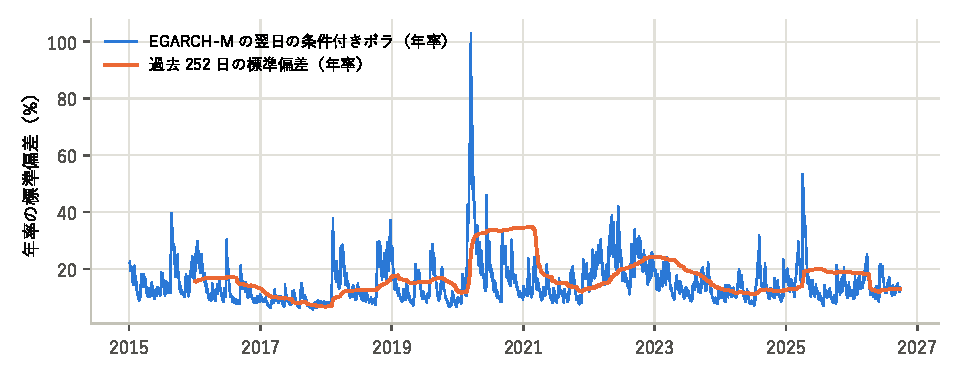
\includegraphics[width=0.95\linewidth]{fig_egarch_vol.pdf}
\caption{EGARCH-M の翌日の条件付きボラティリティ（年率）と、過去 252 日の標準偏差（年率）。}
\label{fig:egarch-vol}
\end{figure}

\tabref{tab:egarch} から分かることを挙げる。

\begin{itemize}
\item 向きへの反応 $\xi=\V{eg.xi}$ は、$t$ 値で $-8$ 程度とはっきり負である。下落の日のあとに、ボラティリティが大きく上がる。
\item 持続性 $\beta=\V{eg.beta}$。ボラティリティの高い状態はしばらく続くが、数週間で戻る。
\item リスクの見返り $\gamma=\V{eg.gamma}$ の $t$ 値は \V{eg.gamma.t} で、0 と区別できない。
\end{itemize}

\figref{fig:egarch-vol} の条件付きボラティリティは、\V{eg.argmax} に年率 \V{eg.max}\% まで上がった。過去 252 日の標準偏差は、その動きにかなり遅れてついていく。

\section{平均の式をそのままビューにすると}

EGARCH-M の平均の式~\eqref{eq:egarch-mean} は、翌日の期待リターン $c+\gamma\sigma_{t+1}$ を出す。これを 21 倍して翌月の予想にすると、中央値は \V{eg.mu.med}\% だが、最小 \V{eg.mu.min}\%、最大 \V{eg.mu.max}\% と、ボラティリティが高い時期に極端に大きくなる。$\gamma>0$ の推定値のもとでは、「危ないときほど期待リターンが高い」という予想になるからである。

これは理屈としては「リスクの高いときにはリスクプレミアムが高い」を表しているが、$\gamma$ は有意でなく、推定の誤差が大きい。このまま BL のビューにすると、危機のさなかに強い強気のビューを置くことになる。マクロのモデルの平均の式からビューを作るときは、

\begin{itemize}
\item 平均の式の係数が有意かを確かめる。有意でなければ、平均の予想は使わない（均衡のまま）。
\item 予想が過去の範囲から大きく外れる時期は、ビューを入れないか、上限を置く。
\item 予想の当たり具合（IC、較正の傾き）を、過去のデータで確かめてから採用率を決める（\chapref{ch:accuracy}）。
\end{itemize}

ことが必要である。

\section{条件付き分散で $\Omega$ を決める}

調査メモは、EGARCH-M の 1 期先の条件付き分散を $\Omega$ の対角にすれば、ボラティリティが急に上がる局面では自動的にビューの確信が下がり、均衡のほうへ戻る「自己修復」の仕組みになる、と述べている。この考え方を確かめる。

採用率は、$\Omega$ と $\tau\Sigma$ の比で決まる。$\Omega$ を条件付き分散 $\sigma_{t+1|t}^2$ に比例させ、$\tau\Sigma$ を過去 252 日の分散 $v_{252,t}$ に比例させると、比例の定数をそろえたとき、採用率は
\begin{equation}
s_t=\frac{v_{252,t}}{v_{252,t}+\sigma^2_{t+1|t}}
\end{equation}
となる。ふだん（2 つが同じくらい）は 50\% である。

\begin{figure}[htbp]
\centering
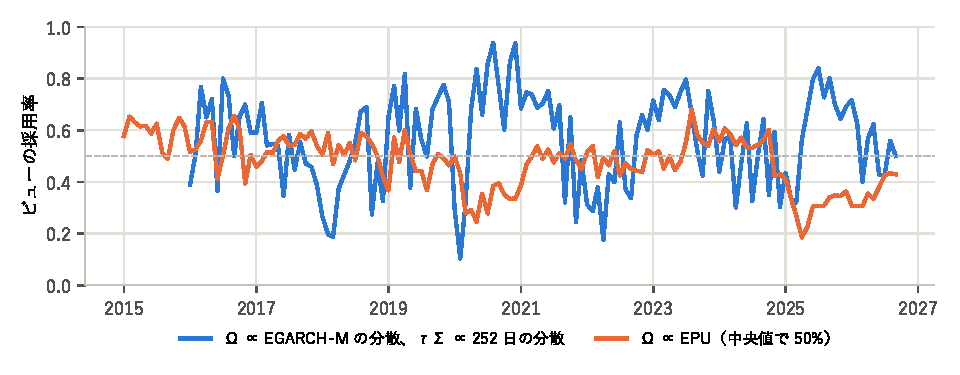
\includegraphics[width=0.95\linewidth]{fig_adoption_time.pdf}
\caption{$\Omega$ をボラティリティの見込みで伸び縮みさせたときの採用率（月末）。青は EGARCH-M の条件付き分散と過去 252 日の分散の比、橙は EPU の水準（中央値で 50\%）。}
\label{fig:adoption-time}
\end{figure}

\figref{fig:adoption-time} の青の線は、次のことを示している。

\begin{itemize}
\item ボラティリティが急に上がった 2020 年 2 月末には、条件付き分散が過去 252 日の分散をはるかに上回り、採用率は \V{eg.adopt.min}\% まで下がった。調査メモの言う「自己修復」である。
\item ところが、危機のあとの 2020 年 8 月には、過去 252 日の分散に危機の時期が含まれる一方で、条件付き分散は下がっているため、採用率は \V{eg.adopt.max}\% まで上がった。危機が去った直後に、ビューをいちばん強く信じる設定になる。
\end{itemize}

採用率の動きは、$\Omega$ と $\Sigma$ を「どれだけ速く動かすか」の差から生まれている。$\Sigma$ も GARCH のような速い見込みで動かせば、2 つは同じように動き、採用率はほとんど変わらない。逆に、$\Sigma$ を長い期間で推定したまま $\Omega$ だけを速く動かすと、危機の始まりでビューを捨て、危機の直後にビューを強く信じることになる。

これが望ましいかどうかは、ビューの当たり具合が局面でどう変わるかによる。危機の直後に予想が当たりやすいという根拠がなければ、意図しない動きである。

\begin{tipbox}[コツ：ボラティリティで $\Omega$ を動かすとき]
\begin{enumerate}
\item 採用率を動かしているのは $\Omega$ と $\tau\Sigma$ の比である。$\Omega$ だけを動かすと、$\Sigma$ との速さの違いがそのまま採用率の動きになる。
\item 「ボラティリティが高いときは予想が外れやすい」だけなら、$\Omega$ と $\Sigma$ を同じ速さで動かすので十分である。採用率は変わらず、比率の傾きはリスクに応じて小さくなる。
\item 「ボラティリティが高いときは、予想の当たり具合（IC）そのものが下がる」と考えるなら、それを過去のデータで確かめ、IC の変化として採用率に入れる。
\end{enumerate}
\end{tipbox}

\section{景気の局面のビュー}

調査メモは、景気循環の局面（拡大、後退など）を特定し、その局面での各資産クラスの過去の平均超過リターンをビューにし、CVaR を最小にする最適化と組み合わせた「CVaR-BL-MCV」というモデルが、年金の配分でシャープレシオを平均 19.7\% 改善した、と紹介している。この資料では、この名前のモデルと数字を述べた論文を見つけられなかった（\appref{app:check}）。近い研究として、上の Sun・Wu・De（2023）の TVC-BL（シャープレシオが 10.5〜13.0\% 改善）と、CVaR を使う BL の研究（\chapref{ch:cop}、\chapref{ch:cvar}）がある。

局面のビューを作るときの一般的な注意を挙げる。

\begin{itemize}
\item \textbf{局面の数が少ない}：アメリカの景気後退は、戦後で十数回しかない。局面ごとの平均リターンは、少ない例の平均で、誤差が大きい。$\Omega$ はその誤差に見合う大きさにする。
\item \textbf{局面の判定の先読み}：景気後退の公式の日付（NBER）は、数か月から 1 年以上あとに発表される。過去の検証で公式の日付を使うと、その時点では分からなかった情報を使うことになる。判定には、その時点で手に入ったデータだけを使う。
\item \textbf{局面の確率}：局面がはっきりしない時期は、局面ごとのビューを確率で重み付けし、局面の不確かさも $\Omega$ に入れる。
\end{itemize}

\section{マクロのファクターモデル}

マクロの変数をファクターとして使い、ファクターへのビューを置く方法もある（\chapref{ch:shape}）。Chen、Roll、Ross（1986）は、鉱工業生産、インフレの予想外の変化、長短金利差、信用スプレッドなどが、株式のリターンに価格付けされたファクターであることを示した。「景気が予想より強い」というビューを鉱工業生産のファクターに置けば、各資産への影響は露出を通じて一貫した形で決まる。ファクターのプレミアムの事前分布と当たり具合を、長いデータで測れるのも利点である。

\begin{keybox}[この章のまとめ]
\begin{itemize}
\item マクロのモデルは、平均の予想（$Q$）とボラティリティの予想（$\Omega$、$\Sigma$）の両方に使える。
\item \SP{} の EGARCH-M では、下落への非対称な反応ははっきりしていたが、リスクの見返り $\gamma$ は有意でなかった。平均の式をビューにすると、危機の時期に極端な強気になる。
\item 条件付き分散で $\Omega$ だけを動かすと、危機の始まりに採用率が \V{eg.adopt.min}\% まで下がる一方、危機の直後に \V{eg.adopt.max}\% まで上がる。$\Omega$ と $\Sigma$ の速さをそろえるかどうかを意識して決める。
\item 景気の局面のビューは、局面の数の少なさと、判定の先読みに注意する。
\end{itemize}
\end{keybox}

% ============================================================
\chapter{財務と ESG}\label{ch:esg}

財務のデータ（割安さ、収益性、投資）と ESG の点数は、銘柄の性質を表す情報である。BL では、こうした性質を (1) ファクターのプレミアムと露出からビューを作る、(2) 均衡や事前分布の目標を調整する、(3) 共分散やリスクの側を調整する、のいずれかで入れられる。この章では、Fama--French のファクターへのビューを数値例で示し、ESG については、調査メモの「共分散を ESG の点数で膨らませる」方法を検討する。

\section{ファクターのプレミアムからビューを作る}

Fama と French（1993、2015）のファクターモデルは、株式のリターンを、市場、規模（SMB）、割安さ（HML）、収益性（RMW）、投資（CMA）のファクターで説明する。これにモメンタム（Carhart 1997）を加えた 6 ファクターがよく使われる。

ファクターを使ってビューを作る方法は 2 つある。

\begin{enumerate}
\item \textbf{銘柄ごとの絶対ビュー}：露出 $B$ とファクターのプレミアムの見込み $\hat\mu_f$ から、$Q=B\hat\mu_f$ を作る。調査メモの「Fama--French の回帰の結果をビューにする」はこの形である。ただし、ファクターの見込みが外れると全銘柄の予想が同じ向きに外れるので、$\Omega$ を対角にしてはいけない（外れの共分散は $B\,\Var(\hat\mu_f)\,B\T$）。
\item \textbf{ファクターへのビュー}：ファクターのプレミアム $\mu_f$ に事前分布を置き、ファクターへのビューで更新する（\chapref{ch:shape}、Kolm and Ritter 2017）。外れの相関が自然に入る。
\end{enumerate}

ここでは 2 番目の方法を、本プロジェクトのセクター ETF（データが長くそろう 9 セクター）と、Kenneth French のデータの 6 ファクターで試す。

\subsection*{設定}

\begin{itemize}
\item \textbf{露出 $B$}：セクター ETF の月次の超過リターンを、6 ファクターに回帰して推定する（2015 年 2 月〜2026 年 8 月の \V{fac.n} か月）。6 ファクターは、セクターの分散の平均 \V{fac.share}\% を説明する。
\item \textbf{事前分布}：ファクターのプレミアムの事前の平均 $\xi$ は、1963 年 7 月〜2014 年 12 月の \V{fac.Tlong} か月の平均（評価期間と重ならない）。モメンタムは年率 \V{fac.mom.prior}\% である。事前の不確かさは $V=F_{\mathrm{long}}/T_{\mathrm{eff}}$（$F_{\mathrm{long}}$ は同じ期間のファクターの共分散）とし、$T_{\mathrm{eff}}$ を変えて事前分布の強さを変える。
\item \textbf{ビュー}：「これからの 12 か月、モメンタムのプレミアムは 0 になる」（モメンタムの急落を心配する、という見方）。不確かさは、12 か月の平均の標準誤差 $\omega=F_{\mathrm{mom}}/12$ とした。
\end{itemize}

\begin{table}[htbp]
\centering
\caption{事前分布の強さ $T_{\mathrm{eff}}$ と、モメンタムへのビューの効き方（年率 \%）。右の 5 列は、ほかのファクターのプレミアムの事後の変化。$T_{\mathrm{eff}}=\V{fac.Tlong}$ は 1963〜2014 年の全データを信じる場合。}
\label{tab:fac-prior}
\tabin{fac_prior}
\end{table}

\tabref{tab:fac-prior} から分かることを挙げる。

\begin{itemize}
\item 事前分布を全データの長さ（$T_{\mathrm{eff}}=\V{fac.Tlong}$ か月）で信じると、12 か月分の見込みのビューの採用率は 1.9\% しかない。50 年分の平均は、1 年分の見込みでは動かない。$\tau\approx1/T$ の考え方（\chapref{ch:tau}）を、ファクターの単位で見たものである。
\item $T_{\mathrm{eff}}=120$（10 年分の確かさ）なら採用率は \V{fac.adopt120}\%、36 か月なら 25\% になる。ファクターのプレミアムは時代とともに変わるので、全データを信じすぎないほうがよい、という判断で $T_{\mathrm{eff}}$ を短くする。
\item モメンタムのプレミアムを下げるビューは、ほかのファクターのプレミアムも動かす。事前の不確かさ $V$ がファクターの共分散に比例しているため、モメンタムと負の相関を持つ市場やバリューのプレミアムが少し上がる。
\end{itemize}

\begin{table}[htbp]
\centering
\caption{$T_{\mathrm{eff}}=120$ のときの、セクターの期待超過リターン（年率 \%）。事前は $B\xi$、事後は $B\mu_f^{\mathrm{post}}$（ファクターで説明できない部分は 0 とした）。}
\label{tab:fac-assets}
\tabin{fac_assets}
\end{table}

\tabref{tab:fac-assets} のとおり、モメンタムへの露出が負のエネルギー（モメンタムの $\beta$ が $-0.36$）は期待リターンが上がり、露出が正の公益は下がる。1 つのファクターへのビューが、露出を通じて全セクターに一貫した形で効く。変化の大きさは年率で 0.5\% 以下と小さいが、これは事前分布が強く、ビューの採用率が 9\% 程度だからである。

\begin{tipbox}[コツ：ファクターへのビュー]
\begin{enumerate}
\item ファクターのプレミアムには長い歴史があるので、事前分布をデータで作れる。ただし、全データをそのまま信じると、どんなビューもほとんど効かない。プレミアムが時代とともに変わることを考えて、事前分布の強さ（$T_{\mathrm{eff}}$）を決める。
\item ビューの不確かさは、ビューの期間の平均の標準誤差（$F/\text{月数}$）が出発点になる。
\item 銘柄ごとのビュー $Q=B\hat\mu_f$ にするなら、外れの共分散 $B\,\Var(\hat\mu_f)B\T$ を $\Omega$ に入れる。対角にしない。
\end{enumerate}
\end{tipbox}

\section{割安さ・収益性などの銘柄の指標}

本プロジェクトは、銘柄ごとの PER、PBR、ROE、売上の伸びなどの指標を DB に持っている（『総合報告書』の「銘柄の指標」の章）。こうした指標をビューにするには、次の手順が素直である。

\begin{enumerate}
\item 指標をセクターの中で順位にし、点数 $z$ に直す（業種によって意味が変わる指標は、業種の中で比べる）。
\item 過去のデータで、点数と翌月のリターンの IC を測る。
\item Grinold の式 $\alpha=\IC\cdot\sigma\cdot z$ で期待リターンのずれにし、$\Omega$ は $\omega=\sigma^2(1/\IC^2-1)$（市場版）、または $\Omega\propto\Sigma$ で採用率 $\IC^2$ にする（\chapref{ch:accuracy}）。
\end{enumerate}

LLM に指標を渡して予想させても、予想はほとんど変わらなかった（『総合報告書』実験 D）。指標をビューにするなら、LLM を通さず、統計的な点数として直接入れるほうが、当たり具合を測りやすい。

\subsection*{本プロジェクトの指標の当たり具合}

本プロジェクトの DB の銘柄の指標（\code{stock\_metrics}）で、各月末の指標の順位と、翌月のリターンの順位相関（IC）を測った。期間は \V{tic.start}〜\V{tic.end} の月末、対象はその時点の \SP{} の構成銘柄である。割安さは、PER・PBR が低いほど高い点数になる向きにした。

\begin{table}[htbp]
\centering
\caption{銘柄の指標の IC（翌月のリターンとの順位相関の、月ごとの値の平均）。採用率は $\IC^2$、右端は Grinold の式で、月次の標準偏差 8\% の銘柄の点数が 1 標準偏差離れているときの期待リターンのずれ（月次 \%）。}
\label{tab:stock-ic}
\tabin{stock_ic}
\end{table}

\begin{figure}[htbp]
\centering
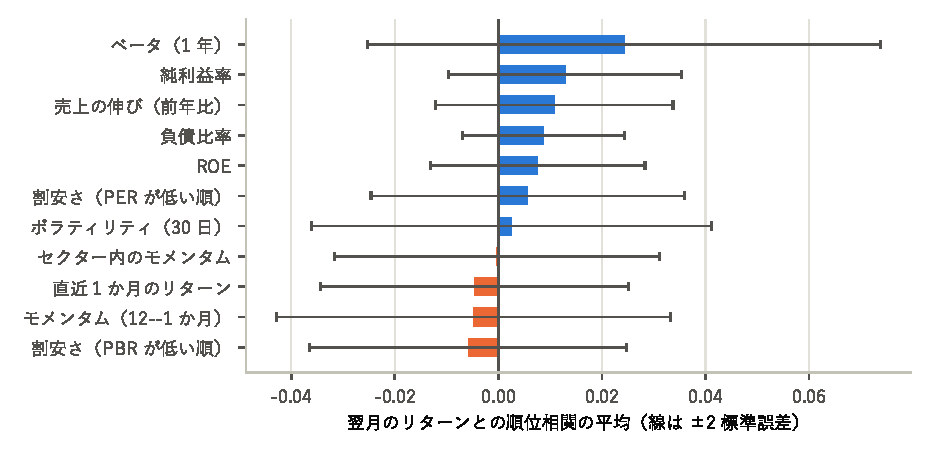
\includegraphics[width=0.9\linewidth]{fig_stock_ic.pdf}
\caption{銘柄の指標の IC の平均と、その ±2 標準誤差。}
\label{fig:stock-ic}
\end{figure}

\tabref{tab:stock-ic} と\figref{fig:stock-ic} のとおり、どの指標も IC の平均は絶対値で 0.025 以下で、$t$ 値が 2 を超えるものはなかった。いちばん大きいのはベータ（\V{tic.beta_1y.mean}、$t$ 値 \V{tic.beta_1y.t}）で、上昇相場の多かった期間に、市場に敏感な銘柄が少し勝ったことを表しているにすぎない。12--1 か月のモメンタムは \V{tic.momentum_12m.mean}、割安さ（PER）は \V{tic.pe_trailing.mean} で、この期間の大型株では、よく知られたファクターも単独ではほとんど効いていない。

この表は、BL のビューの大きさについて、はっきりした教訓を与える。単独の指標の IC が 0.01 程度なら、採用率は 0.01\% のオーダーで、期待リターンはほとんど動かすべきでない。指標を組み合わせて IC を上げるか、効く局面を見分けられない限り、「指標を見て期待リターンを大きく動かす」のは、当たり具合に見合わない。逆に、本プロジェクトの LLM の予想の IC（30 か月で 0.05 程度）は、この表のどの指標より大きい。ただし期間が短く、偶然と区別できない（\chapref{ch:project}）。

\section{ESG を BL に入れる方法}

ESG の点数は、期待リターンの情報か、リスクの情報か、それとも投資家の好み（制約）か。答えによって、入れ方が変わる。

\begin{description}[leftmargin=2em,style=nextline]
\item[好み・制約として] Pedersen、Fitzgibbons、Pomorski（2021）は、ESG を気にする投資家の最適な比率を「ESG 効率的フロンティア」で表した。ESG の点数を、ポートフォリオの平均の ESG の点数の下限などの制約として最適化に入れるのが、いちばん素直である。
\item[期待リターンの目標として] Alpern と Rachev（2025）は、ESG の点数を、期待リターンの Stein 型の縮小推定の目標として使う（$m_i=(1-\lambda)\mu_i+\lambda\xi_i$、$\xi_i$ は ESG の点数）。さらに、均衡の比率を、ダウ平均の比率と ESG の点数に比例する比率の混合 $w_{\mathrm{eq}}=(1-\lambda)w_C+\lambda w_\xi$ にする。リスクは、正規逆ガウス分布（NIG）の多変量版で CVaR を測る。2017〜2021 年のダウ平均の 28 銘柄で、回転率に罰則を付けた戦略のいくつかが年率 40〜45\% になったと報告しているが、多くの組み合わせを試した結果で、標本外の検証は ESG のデータが短いためにできていないと著者自身が述べている。
\item[共分散の構造として] Zuber（2017）の修士論文は、BL の共分散の構造を変えて、ESG の点数に応じて比率を動かす方法を提案している。
\end{description}

\section{共分散を ESG で膨らませる案}\label{sec:esg-penalty}

調査メモは、ESG の点数（0〜1、1 が最高）を使って、共分散を
\begin{equation}
\tilde\Sigma_{ij}=\Sigma_{ij}\sqrt{(2-\mathrm{ESG}_i)(2-\mathrm{ESG}_j)}
\label{eq:esg-penalty}
\end{equation}
と膨らませ、BL の $\Sigma$ に使う方法を紹介している。点数が 1 の銘柄はそのまま、0 の銘柄は分散が 2 倍になる。この資料では、この式を提案した論文を見つけられなかった（\appref{app:check}）。ここでは、式の性質を確かめる。

式~\eqref{eq:esg-penalty} は、$D=\diag(\sqrt{2-\mathrm{ESG}_i})$ として $\tilde\Sigma=D\Sigma D$ と書ける。各銘柄の標準偏差を $\sqrt{2-\mathrm{ESG}_i}$ 倍にし、相関は変えない、という操作である。

\subsection*{均衡と最適化で同じ $\tilde\Sigma$ を使うと、何も変わらない}

BL の手順どおりに、均衡リターンも $\tilde\Pi=\delta\tilde\Sigma\wmkt$ で作り直すと、ビューがないときの比率は $(\delta\tilde\Sigma)^{-1}\tilde\Pi=\wmkt$ で、時価総額の比率のままである。\chapref{ch:prior} で見たとおり、$\Sigma$ に何をしても、均衡と最適化で同じものを使う限り、出発点の比率は変わらない。調査メモの「最適化はボラティリティの制約を避けるために低 ESG の銘柄の比率を自動的に減らす」は、この場合には起きない。

\subsection*{均衡を元の $\Sigma$ のままにすると、比率が動く}

均衡リターンを元の $\Sigma$ で作り（$\Pi=\delta\Sigma\wmkt$）、最適化だけを $\tilde\Sigma$ で行うと、比率は動く。これは、「ESG の低い銘柄は、市場が思っているより危ない」という見方を入れたことになる。

\begin{table}[htbp]
\centering
\caption{4 資産の例（標準偏差 20〜30\%、相関 0.5、$\delta=2.5$）。(1) 均衡も最適化も $\tilde\Sigma$、(2) 均衡は $\Sigma$、最適化は $\tilde\Sigma$（空売りなし・全額投資）。採用率は、各資産に絶対ビューを 1 つずつ置き、$\omega=0.04^2$、$\tau=0.05$ で固定したときの 1 資産あたりの値。右端は Alpern--Rachev の比率の混合（$\lambda=0.25$）。}
\label{tab:esg}
\tabin{esg}
\end{table}

\tabref{tab:esg} の (1) の列は時価総額の比率と一致し（差は最大 \V{esg.w1diff}\%）、(2) の列では、ESG の低い資産 D の比率が 0 になり、高い資産 A が増える。

\subsection*{ビューの採用率は、ESG の低い銘柄で上がる}

もう 1 つ、意図と逆の効果がある。$\Omega$ を外から固定していると、$\tau\tilde\Sigma$ が大きくなった銘柄ほど、均衡の不確かさが大きくなり、ビューの採用率が上がる（\tabref{tab:esg} の採用率の 2 列）。ESG の低い銘柄 D では、採用率が 73.8\% から 84.2\% に上がる。「ESG の低い銘柄は危ないので控えめに」という意図に反して、その銘柄についてのビュー（強気でも弱気でも）を強く信じることになる。

\begin{tipbox}[コツ：ESG を入れるとき]
\begin{enumerate}
\item ESG を共分散で表すなら、均衡を作る $\Sigma$ と最適化の $\Sigma$ のどちらに入れるのかをはっきりさせる。両方に入れると何も変わらない。
\item $\Omega$ を固定したまま共分散を膨らませると、その銘柄のビューの採用率が上がる。意図と逆になりうる。
\item ESG が投資家の好みなら、制約（ポートフォリオの平均の点数の下限、除外）で入れるのが素直である。期待リターンの情報だと考えるなら、ビューや均衡の目標として入れ、当たり具合を確かめる。
\end{enumerate}
\end{tipbox}

\begin{keybox}[この章のまとめ]
\begin{itemize}
\item ファクターへのビューは、露出を通じて全資産に一貫して効き、外れの相関も自然に入る。事前分布を長いデータで信じすぎると、ビューはほとんど効かない。
\item 銘柄の指標は、IC を測ってから Grinold の式で期待リターンに直すのが素直である。
\item 共分散を ESG で膨らませる案は、均衡と最適化で同じ共分散を使うと効かず、均衡を元のままにすると比率が動く。$\Omega$ を固定していると、ESG の低い銘柄のビューを強く信じる方向に働く。
\end{itemize}
\end{keybox}

% ============================================================
\chapter{モメンタム}\label{ch:momentum}

モメンタムは、過去によく上がった銘柄が、その後もしばらく上がりやすいという傾向である。研究の歴史が長く、ビューの材料として使いやすい一方で、まれに大きく崩れる（急落する）。この章では、モメンタムの性質と急落を Kenneth French のデータで確かめ、急落を和らげるボラティリティの調整を再計算する。そのうえで、セクターのモメンタムを BL のビューにして試す。最後に、LLM の予想が先月の値動きの写しになっていること（『総合報告書』）を、モメンタムの観点から読み直す。

\section{モメンタムの研究}

\begin{itemize}
\item Jegadeesh と Titman（1993）は、過去 3〜12 か月によく上がった銘柄を買い、下がった銘柄を売る戦略が、その後 3〜12 か月にわたって利益を上げることを示した。直近の 1 か月は、逆に戻りやすい（短期の反転、Jegadeesh 1990）ので、過去 12 か月から直近 1 か月を除いた「12--1 か月」のリターンで順位を付けるのがふつうである。
\item Carhart（1997）は、これをファクター（UMD）にし、投資信託の成績の説明に使った。Kenneth French のデータのモメンタム・ファクターも、時価総額と過去のリターン（12〜2 か月前）で分けた 6 つのポートフォリオから作られている。
\item Asness、Moskowitz、Pedersen（2013）は、モメンタムが国や資産クラスを越えて見られ、割安さ（バリュー）のファクターと負の相関を持つことを示した。
\end{itemize}

\section{急落}

\begin{paperbox}[Daniel and Moskowitz（2016）, \textit{Momentum Crashes}, Journal of Financial Economics 122(2)]
モメンタムの大きな損失は、まれだが集中して起きる。急落は、市場が大きく下がり、ボラティリティが高い「パニックの状態」のあとで、市場が反発する時期に起きる。下がり続けた銘柄（ベータが高くなっている）が、反発の局面で大きく上がるためである。急落は、ある程度予想できる。
\end{paperbox}

\begin{table}[htbp]
\centering
\caption{モメンタム・ファクターの最悪の月（月次 \%）と、ボラティリティで調整した場合。調整の倍率は、前月末までの 126 取引日の実現ボラティリティから決めた（次の節）。}
\label{tab:mom-worst}
\tabin{mom_worst}
\end{table}

\tabref{tab:mom-worst} のとおり、最悪の月は \V{mom.worst.month} の \V{mom.worst}\% である。2009 年 4 月の \V{mom.2009}\% は、リーマン・ショックのあとの反発の局面で、Daniel と Moskowitz の言う急落の典型である。

\section{ボラティリティで規模を調整する}

\begin{paperbox}[Barroso and Santa-Clara（2015）, \textit{Momentum Has Its Moments}, Journal of Financial Economics 116(1)]
モメンタムのリスク（ボラティリティ）は時期によって大きく変わり、しかも予想しやすい。前月までの 126 取引日の日次リターンから実現ボラティリティを見積もり、目標のボラティリティ（年率 12\%）÷ 見積もり、の倍率でポジションの大きさを決める。1927〜2011 年で、シャープレシオは 0.53 から 0.97 に上がり、急落のリスクが大きく下がった。
\end{paperbox}

この方法を、Kenneth French の日次と月次のモメンタム・ファクターで再計算した。月 $t$ の倍率は、前月末までの 126 取引日の日次リターンの 2 乗の平均に 21 を掛けた月次の分散 $\hat\sigma_t^2$ から、$0.12/\sqrt{12}\,/\,\hat\sigma_t$ とした。

\begin{table}[htbp]
\centering
\caption{モメンタム・ファクターの成績と、ボラティリティで調整した場合（年率 \%、シャープレシオはリスクフリーを引かない比）。尖度は超過尖度。}
\label{tab:mom-bsc}
\tabin{mom_bsc}
\end{table}

\begin{figure}[htbp]
\centering
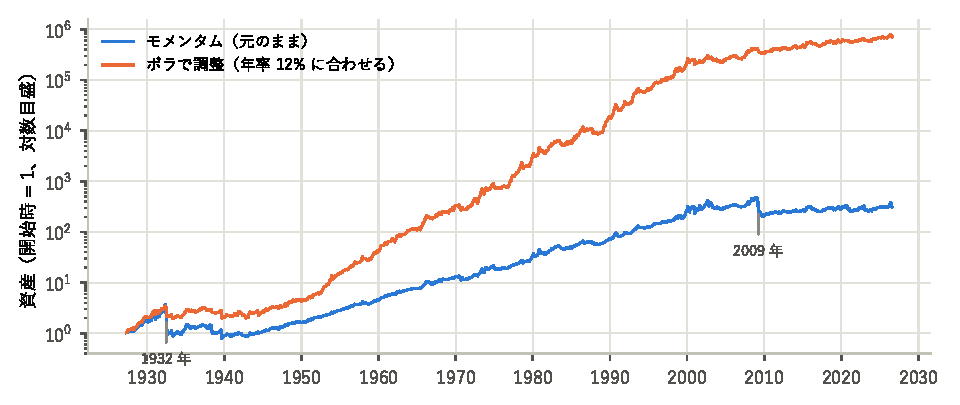
\includegraphics[width=0.95\linewidth]{fig_mom_long.pdf}
\caption{モメンタム・ファクターの累積（対数目盛）。ボラティリティで調整すると、1932 年と 2009 年の急落が小さくなり、長期の成長も大きくなる。}
\label{fig:mom-long}
\end{figure}

\tabref{tab:mom-bsc} と\figref{fig:mom-long} から分かることを挙げる。

\begin{itemize}
\item 1927〜2011 年では、シャープレシオは \V{mom.sh.sub} から \V{mom.sh.sub.sc} に上がった。Barroso と Santa-Clara の 0.53 から 0.97 とほぼ同じである（期間の始まりと、データの版がわずかに違う）。
\item 全期間（\V{mom.start}〜\V{mom.end}）でも、\V{mom.sh.all} から \V{mom.sh.all.sc} に上がった。最大の下落は \V{mom.dd}\% から \V{mom.dd.sc}\% に縮んだ。
\item 2009 年 4 月の倍率は \V{mom.2009.scale} で、損失は \V{mom.2009}\% から \V{mom.2009.sc}\% になった。急落の前に、すでにボラティリティが高くなっていたので、ポジションが小さくなっていた。
\item 2015 年以降のモメンタムは弱く、調整前のシャープレシオは 0.2 程度である。
\end{itemize}

\subsection*{BL の言葉で言うと}

ボラティリティで規模を調整することは、BL では「モメンタムのビューの確信度を、モメンタム自身の最近のボラティリティに応じて変える」ことに当たる。モメンタムの期待リターン（平均）はボラティリティほど大きく変わらないので、ボラティリティの高い時期にはシャープレシオが下がり、ビューの採用率を下げるのが理にかなう。\chapref{ch:macro} で見た「$\Omega$ だけを速く動かす」と違い、ここでは「ボラティリティの高い時期には予想（モメンタムの順位）の価値が下がる」という裏付けがある。

\section{取引戦略をビューにする研究}

\begin{itemize}
\item Fabozzi、Focardi、Kolm（2006）は、モメンタムのような取引戦略を BL のビューとして組み込む枠組みを示した（\textit{Incorporating Trading Strategies in the Black--Litterman Framework}, Journal of Trading 1(2)）。この資料では本文を確認できなかった。
\item Bessler、Opfer、Wolff（2017）は、過去のデータから作るビュー（標本に基づく BL）を、世界の株式・債券・商品の指数（1993〜2011 年）に当てはめた。BL のポートフォリオは、1/N、平均分散、Bayes--Stein、最小分散のどれよりも、標本外のシャープレシオが高かった。リスク回避度、投資の制約、取引費用を変えても同じだった。理由として、期待リターンの見込みが安定し、推定の誤差が小さく、回転率が低いことを挙げている。
\end{itemize}

\section{セクターのモメンタムを BL で試す}

本プロジェクトのセクター ETF（最大 11 セクター）で、モメンタムのビューを BL に入れて検証した。

\begin{itemize}
\item \textbf{期間}：判断日は 2016 年 1 月〜2026 年 8 月の各月末（\V{sm.months} か月）。翌月のリターンで評価する。
\item \textbf{ベンチマーク}：その日の \SP{} の構成銘柄の時価総額をセクターごとに合計した比率（ETF のあるセクターだけ）。
\item \textbf{均衡}：$\Sigma$ は過去 252 日の日次リターンの縮小推定を 21 倍した月次の共分散。$\delta=2.5$。
\item \textbf{点数}：12--1 か月のモメンタムを、セクターの間で標準化した $z$。
\item \textbf{IC}：その月までに分かっている、点数と翌月のリターン（セクターの平均を引く）の相関の平均。最初は 0.05 を 24 か月分の重みで混ぜ、負なら 0 とする。
\end{itemize}

比べた戦略は 3 つである。

\begin{enumerate}
\item \textbf{IC で縮めたビュー}：$\mu=\Pi+\IC_t\cdot\sigma\cdot z$（Grinold の式。市場版の BL で $\omega=\sigma^2(1/\IC^2-1)$ と同じ）。
\item \textbf{IC ＋ ボラティリティで調整}：上の $\IC_t$ に、モメンタム・ファクターのボラティリティの倍率（前の節、上限 1.5）を掛ける。
\item \textbf{過去の平均がそのまま続く}：$\mu=\Pi+(\text{12--1 か月のリターン})/11$。過去 11 か月の月平均のリターンが、そのまま来月も続くとみる（採用率 100\%）。
\end{enumerate}

どれも、空売りなし・全額投資で $\mu\T w-\frac{\delta}{2}w\T\Sigma w$ を最大にした。

\begin{figure}[htbp]
\centering
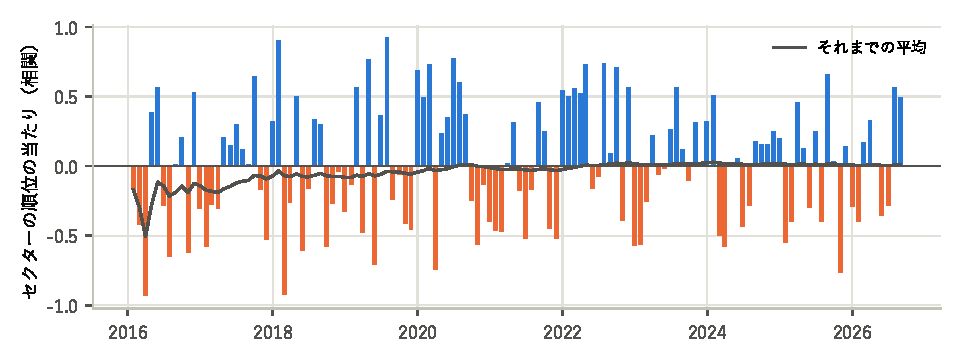
\includegraphics[width=0.95\linewidth]{fig_secmom_ic.pdf}
\caption{セクターのモメンタムの当たり具合（月ごとの、点数と翌月のリターンの相関）と、それまでの平均。}
\label{fig:secmom-ic}
\end{figure}

\begin{table}[htbp]
\centering
\caption{セクターのモメンタムの BL（\V{sm.start}〜\V{sm.end}、年率 \%）。TE と IR はベンチマークに対するもの、$t$ 値は月次の超過リターンの平均の $t$ 値、回転率は月平均、実質数は $1/\sum w^2$ の平均。}
\label{tab:secmom}
\tabin{secmom}
\end{table}

\begin{figure}[htbp]
\centering
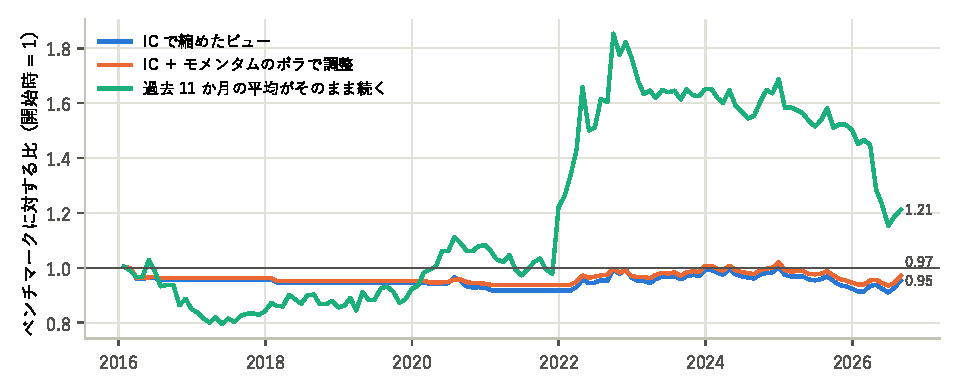
\includegraphics[width=0.95\linewidth]{fig_secmom_cum.pdf}
\caption{ベンチマークに対する累積の比。}
\label{fig:secmom-cum}
\end{figure}

結果は次のとおりである。

\begin{itemize}
\item セクターのモメンタムの当たり具合は、平均 \V{sm.cic.mean}（$t$ 値 \V{sm.cic.t}、128 か月のうち \V{sm.cic.pos} か月がプラス）で、ほとんど 0 だった（\figref{fig:secmom-ic}）。セクターは 10 前後しかないので、月ごとの相関は $\pm1$ の近くまで大きくぶれる。
\item IC で縮めたビューは、採用率がほとんど 0 になるので、ベンチマークに近い比率になった。TE は \V{sm.icv.te}\%、IR は \V{sm.icv.ir}（$t$ 値 \V{sm.icv.t}）。ボラティリティで調整した版も同じような結果である。
\item 過去の平均がそのまま続くとみる戦略は、実質 1 セクター程度に集中し、TE は \V{sm.naive.te}\% と大きい。2022 年に大きく勝ち（この年はエネルギーのセクターが大きく上がった）、その後に負けを重ねた（\figref{fig:secmom-cum}）。IR は \V{sm.naive.ir}（$t$ 値 \V{sm.naive.t}）で、偶然と区別できない。
\end{itemize}

当たり具合が 0 に近いビューを正しく縮めると、BL はほとんど何もしない。これは失敗ではなく、BL が設計どおりに働いた結果である。逆に、縮めずに入れた戦略の大きな勝ち負けは、ビューの価値ではなく、集中の結果である。

\section{LLM の予想と短期の反転}

『総合報告書』で見たとおり、本プロジェクトの LLM の予想は、渡した月の平均リターンとの相関が平均 \V{llm.cin.mean} で、先月の値動きをほぼ写している。これは「直近 1 か月の値動きがそのまま続く」という、1 か月のモメンタムの予想である。

モメンタムの研究は、12--1 か月のモメンタムを使い、直近の 1 か月をわざわざ除く。個別の銘柄では、直近 1 か月によく上がった銘柄は翌月に戻りやすい（短期の反転、Jegadeesh 1990、Lehmann 1990）からである。LLM の予想は、この反転とは逆の向きに賭けていることになる。

ただし、本プロジェクトの DB で 2015〜2026 年の \SP{} の構成銘柄を調べると、直近 1 か月のリターンと翌月のリターンの順位相関は \V{tic.return_1m.mean}（$t$ 値 \V{tic.return_1m.t}）で、反転も継続もほとんど見られなかった（\chapref{ch:esg} の\tabref{tab:stock-ic}）。12--1 か月のモメンタムも \V{tic.momentum_12m.mean} で、効いていない。LLM の予想の当たり具合は弱い正（順位相関 \V{llm.ic.mean}）で、少なくとも 2024〜2026 年には反転に負けてはいなかった。それでも、「先月の写し」のビューに大きな確信を置く根拠は、モメンタムの研究からも、この期間のデータからも出てこない。

\begin{tipbox}[コツ：モメンタムのビュー]
\begin{enumerate}
\item 順位は 12--1 か月のリターンで付ける。直近の 1 か月は、個別の銘柄では反転しやすい。
\item ビューの大きさは IC で決める。モメンタムの IC は時期によって大きく変わり、最近 10 年は弱い。
\item モメンタム自身の最近のボラティリティが高いときは、確信度を下げる（Barroso and Santa-Clara の倍率）。急落は、下げ相場のあとの反発で起きやすい。
\item 勝ち組と負け組の差（相対ビュー）で入れ、市場全体の方向の賭けを混ぜない。
\item 縮めずに入れると、比率は少数の資産に集中し、成績は集中の結果になる。
\end{enumerate}
\end{tipbox}

\begin{keybox}[この章のまとめ]
\begin{itemize}
\item モメンタムは、まれに大きく急落する（最悪の月は \V{mom.worst}\%）。急落は、下げ相場のあとの反発の局面で起きる。
\item 実現ボラティリティで規模を調整すると、シャープレシオは \V{mom.sh.all} から \V{mom.sh.all.sc} に上がり、最大の下落は \V{mom.dd}\% から \V{mom.dd.sc}\% に縮んだ。BL では、確信度をモメンタムのボラティリティで動かすことに当たる。
\item セクターのモメンタムは 2016〜2026 年にはほとんど当たらず、正しく縮めた BL はベンチマークの近くにとどまった。
\item LLM の「先月の写し」の予想は、1 か月のモメンタムの賭けで、個別株の短期の反転とは逆の向きである。
\end{itemize}
\end{keybox}


\part{正規分布を越える拡張と、最適化での使い方}
% ============================================================
\chapter{エントロピー・プーリング}\label{ch:ep}

BL は、市場もビューも正規分布で、ビューは期待リターンの線形の組み合わせ、という枠の中で働く。実際には、リターンの分布は裾が厚く、左右対称でもない。言いたいビューも、「A は B より上」（順位）、「この資産のボラティリティは今より大きい」、「10\% 以上下がる確率は 3\%」のように、平均の線形の組み合わせではないことが多い。

Meucci（2008）のエントロピー・プーリング（Fully Flexible Views）は、こうしたビューを、どんな分布の市場にも入れられる方法である。この章では、考え方と解き方を説明し、セクター ETF の例で計算する。

\section{BL の枠を越える必要}

Meucci（2010）は、BL とその拡張が扱えることを\tabref{tab:meucci-cap}のように整理している。

\begin{table}[htbp]
\centering
\caption{BL と拡張が扱えること（Meucci 2010 の表を日本語にしたもの）。BL：元の BL と市場版、AC：Almgren and Chriss（2006）、QG：Qian and Gorman（2001）、P：Pezier（2007）、M：Meucci（2009）、COP：コピュラ・オピニオン・プーリング（Meucci 2006）、EP：エントロピー・プーリング（Meucci 2008）。}
\label{tab:meucci-cap}
\small
\begin{tabular}{lccccccc}
\toprule
 & BL & AC & QG & P & M & COP & EP \\
\midrule
正規分布の市場と線形のビュー & $\checkmark$ & & $\checkmark$ & $\checkmark$ & $\checkmark$ & $\checkmark$ & $\checkmark$ \\
シナリオ分析 & $\checkmark$ & & $\checkmark$ & $\checkmark$ & $\checkmark$ & $\checkmark$ & $\checkmark$ \\
相関のストレステスト & & & $\checkmark$ & $\checkmark$ & $\checkmark$ & & $\checkmark$ \\
非線形の価格付け（デリバティブ） & & & & & $\checkmark$ & $\checkmark$ & $\checkmark$ \\
外部の要因（マクロなど） & & & & & $\checkmark$ & $\checkmark$ & $\checkmark$ \\
部分的な指定 & & & & $\checkmark$ & $\checkmark$ & & $\checkmark$ \\
正規分布でない市場 & & & & & & $\checkmark$ & $\checkmark$ \\
複数の利用者 & & & & & & $\checkmark$ & $\checkmark$ \\
非線形のビュー & & & & & & & $\checkmark$ \\
価格付けの重いデリバティブ & & & & & & & $\checkmark$ \\
緩い制約（順位） & & $\checkmark$ & & & & & $\checkmark$ \\
\bottomrule
\end{tabular}
\end{table}

エントロピー・プーリングは、表のすべての列に印が付く。仕組みは単純で、市場の分布を多数のシナリオで表し、ビューを満たすように「シナリオの確率」だけを変える。

\section{シナリオと確率}

事前の市場の分布を、$J$ 個のシナリオ $x_1,\dots,x_J$（各 $N$ 次元）と、その確率 $p_1,\dots,p_J$ で表す。シナリオは、過去のリターンそのものでも、モンテカルロ法で作ったものでもよい。正規分布である必要はない。

事後の分布は、同じシナリオに新しい確率 $q_1,\dots,q_J$ を付けたものとする。シナリオの値は変えないので、デリバティブのように価格付けの計算が重いものでも、計算し直す必要がない。

\section{相対エントロピーの最小化}

ビューは、確率 $q$ についての条件として書く。例を挙げる。

\begin{center}
\small
\begin{tabular}{p{4.4cm}p{9.2cm}}
\toprule
ビュー & $q$ についての条件 \\
\midrule
A の期待リターンは 1\% & $\sum_j q_j x_{j,A}=0.01$ \\
A の期待リターンは B 以上（順位） & $\sum_j q_j(x_{j,A}-x_{j,B})\ge0$ \\
A の標準偏差は 1.3 倍（平均は固定） & $\sum_j q_jx_{j,A}=m_A$、$\sum_j q_jx_{j,A}^2=m_A^2+(1.3\sigma_A)^2$ \\
A が $-10\%$ 以下になる確率は 3\% & $\sum_j q_j\,\one\{x_{j,A}\le-0.10\}=0.03$ \\
A と B の相関（平均・分散を固定） & $\sum_j q_jx_{j,A}x_{j,B}=$ 目標の値 \\
\bottomrule
\end{tabular}
\end{center}

どれも $q$ の線形の式（等式か不等式）になる。ビューを満たす $q$ はたくさんあるので、その中から、事前の確率 $p$ に「いちばん近い」ものを選ぶ。近さは相対エントロピー（カルバック・ライブラーの情報量）で測る。
\begin{equation}
\min_{q}\;\sum_{j=1}^J q_j\log\frac{q_j}{p_j}
\quad\text{s.t.}\quad Hq=h,\quad Gq\le g,\quad \sum_j q_j=1
\label{eq:ep}
\end{equation}
相対エントロピーは、「事前の分布から見て、事後の分布がどれだけ意外か」を表す。ビューを満たすのに必要な最小限だけ、確率を動かすことになる。

\section{双対で解く}

式~\eqref{eq:ep} は、変数がシナリオの数 $J$（数万）だけあるが、条件の数 $K$（数個）は少ない。ラグランジュの未定乗数 $\lambda$ を使って、小さな問題に直せる（\appref{app:formulas}）。等式の条件をまとめて $Aq=b$（$\sum q_j=1$ も含む）と書くと、ラグランジュ関数は
\begin{equation}
L(q,\lambda)=\sum_j q_j(\log q_j-\log p_j)+\lambda\T(Aq-b)
\end{equation}
である。$q_j$ で微分して 0 とおくと
\begin{equation}
\log q_j-\log p_j+1+a_j\T\lambda=0\quad\Longrightarrow\quad q_j(\lambda)=p_j\exp\bigl(-1-a_j\T\lambda\bigr)
\label{eq:ep-q}
\end{equation}
となる（$a_j$ は $A$ の $j$ 列目）。これを $L$ に戻すと、双対の関数 $g(\lambda)=-\sum_j q_j(\lambda)-\lambda\T b$ が得られ、これを最大にすればよい。$-g$ は凸で、勾配は $b-Aq(\lambda)$ と簡単に書けるので、準ニュートン法などで $K$ 次元の問題として速く解ける。不等式の条件は、対応する $\lambda$ を 0 以上に制限すれば扱える。

式~\eqref{eq:ep-q} は、事後の確率が「事前の確率 × 条件の式の指数」になることを示している。例えば、平均のビューだけなら $q_j\propto p_j\exp(-\lambda x_{j,A})$ で、ビューの方向のシナリオの確率を指数的に上げる（指数的な傾け、exponential tilting）。

\section{確信度とオピニオン・プーリング}

ビューを 100\% は信じないとき、Meucci は事前と事後の確率を混ぜる。
\begin{equation}
p^{(c)}=(1-c)\,p+c\,q,\qquad 0\le c\le1
\label{eq:ep-pool}
\end{equation}
$c$ は確信度である。複数の人がそれぞれビューを持つときは、それぞれの事後の確率を、信頼の重みで混ぜる（オピニオン・プーリング）。混ぜた確率のもとでの期待値は、事前と事後の期待値の $c$ による内分になる。

\section{数値例：セクター ETF}

\chapref{ch:momentum} のセクター ETF の、最後の判断日（\V{ep.date}）の入力を使う。事前の分布は、平均を均衡リターン $\Pi$（月次）、共分散を $\Sigma$（月次）とする自由度 5 の多変量 $t$ 分布で、裾の厚い分布である。ここから \V{ep.J} 個のシナリオを作り、確率は等しく $1/J$ とした。

ビューは次の 3 つである。

\begin{enumerate}
\item \textbf{順位}：情報技術（XLK）の期待リターンは、公益（XLU）を月 1\% 以上上回る（不等式）。事前の差は \V{ep.spread0}\%。
\item \textbf{ボラティリティ}：エネルギー（XLE）の標準偏差は、事前の 1.3 倍になる（平均は事前のまま）。事前は月次 \V{ep.sdE0}\%。
\item \textbf{下落の確率}：金融（XLF）が月に $-10\%$ 以下になる確率は 3\% である。事前は \V{ep.tail0}\%。
\end{enumerate}

\begin{table}[htbp]
\centering
\caption{エントロピー・プーリングの結果（月次 \%）。「平均のみ」は、ビュー 1 を等式（差がちょうど 1\%）にして、それだけを入れたときの平均の変化。EP はエントロピー・プーリング、BL は同じビューを市場版の BL（$\Omega\to0$）で入れたもの。}
\label{tab:ep}
\tabin{ep}
\end{table}

\begin{figure}[htbp]
\centering
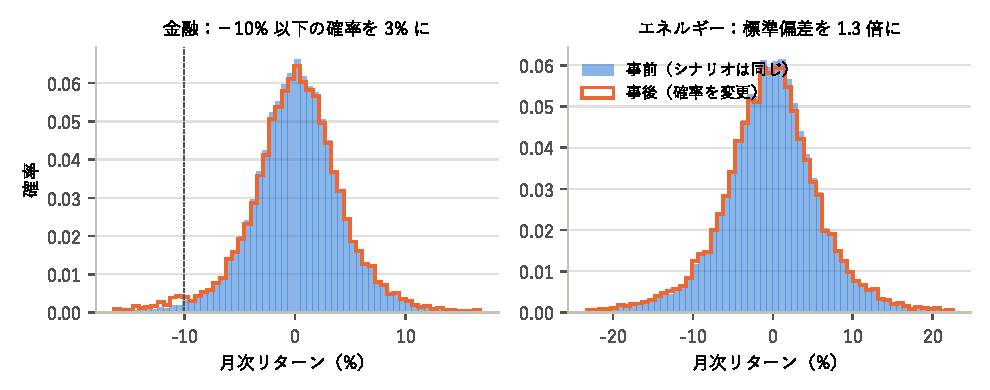
\includegraphics[width=0.95\linewidth]{fig_ep.pdf}
\caption{同じシナリオの、事前の確率（塗り）と事後の確率（線）。左：金融の $-10\%$ 以下の確率を上げると、左の裾の確率が増える。右：エネルギーの標準偏差を上げると、両方の裾の確率が増える。}
\label{fig:ep}
\end{figure}

結果は次のとおりである（\tabref{tab:ep}、\figref{fig:ep}）。

\begin{itemize}
\item 3 つのビューはすべて満たされた。情報技術と公益の差は \V{ep.spread1}\%、金融の下落の確率は \V{ep.tail1}\%、エネルギーの標準偏差は \V{ep.sdE1}\% になった。
\item ビューのない資産の分布も動く。金融の下落の確率を上げると、金融と一緒に下がりやすいシナリオの確率が上がるので、ほとんどのセクターで下落の確率が上がり、平均が下がる。一方、情報技術を押し上げる順位のビューの影響で、情報技術と連動しやすい資本財は平均が上がった。相関の構造は、シナリオを通じてそのまま保たれる。
\item 相対エントロピーは \V{ep.kl}、確率の偏りを表す有効なシナリオの割合（$\exp(-\sum q\log q)/J$）は \V{ep.ens}\% で、確率の変え方は穏やかだった。
\item 確信度 $c=0.5$ で混ぜると、差は \V{ep.c.spread}\%、下落の確率は \V{ep.c.tail}\% になる。
\end{itemize}

\section{平均のビューなら、BL とほぼ同じ}

ビュー 1 を「差がちょうど 1\%」という等式にして、それだけを入れると、エントロピー・プーリングによる平均の変化は、市場版の BL を $\Omega\to0$ で使ったときの変化と、最大 \V{ep.maxdiff}\% の差で一致した（\tabref{tab:ep} の右の 2 列）。

Meucci は、正規分布の市場に線形の平均のビューを入れる場合、エントロピー・プーリングが BL の結果を再現することを示している。今回の事前分布は $t$ 分布だが、平均の条件付けは楕円形の分布ならほぼ同じ形になる。エントロピー・プーリングは BL を置き換えるものではなく、BL を含む広い枠組みである。違いが出るのは、順位、ボラティリティ、裾の確率のような、平均以外のビューを入れたときである。

\section{使うときの注意}

\begin{itemize}
\item \textbf{シナリオの数}：裾のビュー（下落の確率など）は、裾に十分なシナリオがないと満たせないか、少数のシナリオに確率が集中する。有効なシナリオの割合が小さくなったら、シナリオを増やすか、ビューを弱める。
\item \textbf{満たせないビュー}：シナリオの範囲の外のビュー（すべてのシナリオで $-5\%$ より上なのに、「$-10\%$ 以下の確率は 3\%」）は満たせない。双対の解が発散したら、まずこれを疑う。
\item \textbf{不確かさの扱い}：エントロピー・プーリングのビューは、それ自体には不確かさを持たない（満たすか満たさないか）。不確かさは、式~\eqref{eq:ep-pool} の確信度 $c$ で入れる。$c$ も、当たり具合から決めるのが望ましい（\chapref{ch:accuracy}）。
\item \textbf{確率の変化を見る}：事後の確率 $q/p$ の分布を見て、一部のシナリオに極端な重みが付いていないかを確かめる。
\end{itemize}

\begin{tipbox}[コツ：エントロピー・プーリング]
\begin{enumerate}
\item 平均のビューだけなら、BL で十分である。順位、ボラティリティ、裾の確率、相関のビューを入れたいときに使う。
\item 事前のシナリオは、裾の厚さを表せるもの（過去のリターン、$t$ 分布、GARCH のシミュレーション）にする。
\item ビューの不確かさは、確信度 $c$ で事前と事後を混ぜて入れる。
\item 有効なシナリオの割合を確かめ、確率が一部に集中していないかを見る。
\end{enumerate}
\end{tipbox}

\begin{keybox}[この章のまとめ]
\begin{itemize}
\item エントロピー・プーリングは、シナリオの値を変えずに確率だけを変え、ビューを満たす中で事前にいちばん近い（相対エントロピーが最小の）分布を選ぶ。
\item 双対で解けば、条件の数だけの小さな凸の問題になる。事後の確率は、事前の確率に条件の式の指数を掛けたものになる。
\item 順位・ボラティリティ・裾の確率のビューを、裾の厚い分布に入れられる。平均のビューだけなら、BL とほぼ同じ答えになる。
\end{itemize}
\end{keybox}

% ============================================================
\chapter{コピュラ・オピニオン・プーリングと、正規分布でない BL}\label{ch:cop}

エントロピー・プーリングより前に、Meucci（2006）は、正規分布でない市場にビューを入れる方法として、コピュラ・オピニオン・プーリング（COP）を示した。ビューを「値」ではなく「分布」で表し、市場の依存の構造（コピュラ）を保ったまま、ビューの分布を混ぜる方法である。この章では COP の手順を例で示し、そのあと、正規分布でない市場で BL を使う研究（安定分布、コピュラと CVaR、正規分布の混合）を紹介する。

\section{コピュラ}

多変量の分布は、各変数の分布（周辺分布）と、変数どうしのつながり方（コピュラ）に分けて考えられる（Sklar の定理）。各変数を自分の累積分布関数で変換した $U_k=F_k(X_k)$（0〜1 の一様分布になる「順位」）の同時分布がコピュラである。

正規分布の相関は、つながり方のうち、平均的な連動しか表さない。正規分布のコピュラでは、極端に大きく下がるときの連動（裾の依存）は 0 に近づく。実際の市場では、暴落のときにほとんどの資産が一緒に下がる。$t$ 分布のコピュラや、2 変数ずつのコピュラを積み上げる vine コピュラは、この裾の依存を表せる。モメンタムの急落（\chapref{ch:momentum}）のような事象のリスクを測るには、裾の依存が重要になる。

\section{COP の手順}

Meucci の COP は、次の 5 段の手順である。

\begin{enumerate}
\item \textbf{事前の市場}：市場のリターンのシナリオ $X$ を、モンテカルロ法などで $J$ 個作る。分布は何でもよい。
\item \textbf{ビューの座標に回す}：ビューの行列 $P$（$K\times N$）に、残りの方向を表す行 $P_\perp$ を足して、正則な $N\times N$ の行列 $\bar P$ を作る。$V=\bar PX$ の最初の $K$ 個がビューの変数である。
\item \textbf{ビューの分布と確信度}：ビュー $k$ ごとに、ビューの変数の主観的な分布 $\hat F_k$ と確信度 $c_k$ を決め、事前の分布 $F_k$ と混ぜる。
\begin{equation}
\tilde F_k=(1-c_k)\,F_k+c_k\,\hat F_k
\end{equation}
\item \textbf{コピュラを保って置き換える}：各シナリオのビューの変数の順位 $U_k=F_k(V_k)$ はそのままにして、新しい分布の分位点 $\tilde V_k=\tilde F_k^{-1}(U_k)$ に置き換える。順位が変わらないので、ビューの変数とほかの変数のつながり方（コピュラ）は保たれる。
\item \textbf{元の座標に戻す}：$\tilde X=\bar P^{-1}\tilde V$。
\end{enumerate}

ビューを分布で言えるので、「スプレッドは 2\% くらいだが、外れるときは大きく外れる」（裾の厚いビュー）や、「上には大きく、下には小さく」（非対称なビュー）も入れられる。

Meucci 自身は、のちに COP について「場当たり的な操作に頼っている」と述べ、エントロピー・プーリングでその問題を解いた、と位置づけている（Meucci 2010）。とくに、2 段目の補う行 $P_\perp$ の選び方に、決まった答えがない。

\section{数値例}

\chapref{ch:ep} と同じセクター ETF の事前のシナリオ（自由度 5 の多変量 $t$ 分布、\V{ep.J} 個）を使う。ビューは、情報技術と公益の差（スプレッド）について、自由度 4、中心 \V{cop.loc}\%、尺度 \V{cop.scale}\% の $t$ 分布とし、確信度は $c=\V{cop.c}$ とした。補う行は、ビューの行に直交する正規直交の行とした。

\begin{figure}[htbp]
\centering
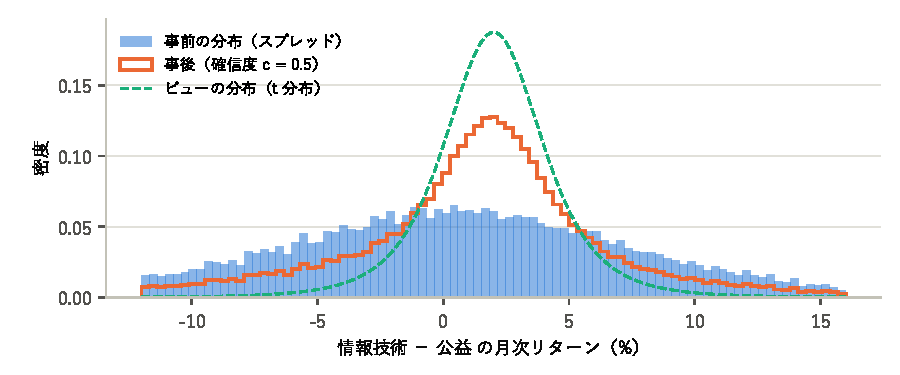
\includegraphics[width=0.92\linewidth]{fig_cop.pdf}
\caption{情報技術 $-$ 公益のスプレッドの、事前の分布、ビューの分布、COP の事後の分布（確信度 0.5）。}
\label{fig:cop}
\end{figure}

\begin{table}[htbp]
\centering
\caption{COP と市場版の BL の、各セクターの期待リターンの変化（月次 \%）。市場版の BL は、スプレッドの平均を COP の事後の平均と同じ値にする条件を付けたもの。}
\label{tab:cop}
\tabin{cop}
\end{table}

結果は次のとおりである（\figref{fig:cop}、\tabref{tab:cop}）。

\begin{itemize}
\item スプレッドの平均は \V{cop.m0}\% から \V{cop.m1}\% に、標準偏差は \V{cop.sd0}\% から \V{cop.sd1}\% になった。事後の分布は、事前の広い分布とビューの尖った分布の混合で、中心が尖り、裾は事前の厚さを残す。5\% 点は \V{cop.q05.0}\% から \V{cop.q05}\% に、95\% 点は \V{cop.q95.0}\% から \V{cop.q95}\% に縮んだ。
\item 期待リターンが動いたのは、情報技術（$+$）と公益（$-$）だけで、ほかのセクターの変化は最大 \V{cop.otherdiff}\% だった。補う行をビューに直交させたので、ほかの方向の変数がそのまま残ったためである。
\item 市場版の BL で同じ大きさの平均の変化を入れると、相関を通じてほかのセクターも動く（情報技術と相関の高い一般消費財や資本財は上がり、公益に近い生活必需品や不動産は下がる）。
\end{itemize}

COP と BL のどちらの動き方が正しい、ということはない。「ほかの資産には何も言っていない」と考えるなら COP のように動かさず、「ほかの資産も、相関に応じて同じ情報の影響を受けるはず」と考えるなら BL のように動かす。COP では補う行の選び方で、この振る舞いを選べる。エントロピー・プーリングでは、平均だけを条件にすれば BL に近い動き方になる（\chapref{ch:ep}）。

\section{正規分布でない市場での BL の研究}

\begin{paperbox}[Giacometti, Bertocchi, Rachev and Fabozzi（2007）, \textit{Stable distributions in the Black--Litterman approach to asset allocation}, Quantitative Finance 7(4)]
均衡の議論を、裾の厚い安定分布の市場に拡張した（Meucci 2010 による紹介）。BL のビューを、裾のリスクの指標（VaR、CVaR）の計算に入れる方法も論じている。
\end{paperbox}

\begin{paperbox}[Teplova, Mikova, Munir and Pivnitskaya（2023）, \textit{Black-Litterman model with copula-based views in mean-CVaR portfolio optimization framework with weight constraints}, Economic Change and Restructuring 56(1)]
\begin{itemize}
\item 10 の国際的な ETF の日次データ（2012〜2022 年）。
\item ARMA-GARCH とコピュラから作った期待リターンを投資家のビューの代わりに使い、リスクは CVaR で測る。多変量のつながりは、柔軟な R-vine コピュラで表す。
\item コピュラに基づく BL（CBL）、コピュラ-CVaR、平均分散、等金額を、比率の上限 30\%、40\%、50\% のもとで、標本外で比べる。ビューへの確信のパラメータ $\tau$ も変える。
\item CBL は裾のリスクが小さく、リスク調整後のリターンが高かった。コピュラ-CVaR は回転率と損益分岐点で優れていた。$\tau$ の値は結果に大きく効いた。
\end{itemize}
\end{paperbox}

\begin{itemize}
\item Alpern と Rachev（2025）は、BL で期待リターンを作り、リスクは多変量のアフィン一般化双曲型分布（正規逆ガウス分布）で CVaR として測った（\chapref{ch:esg}）。
\item 株式のリターンを正規分布の混合で表し、市場の均衡を逆最適化で取り込み、CVaR を最小にする研究もある（\textit{Incorporating Black-Litterman Views in Portfolio Construction when Stock Returns are a Mixture of Normals}, arXiv 1706.03287）。
\end{itemize}

これらの研究に共通するのは、「期待リターンは BL（またはビューに基づく方法）で作り、リスクは裾を表せる分布で測る」という分業である。期待リターンの推定の誤差を BL で抑えつつ、正規分布の仮定が最も効く裾のリスクは、別のモデルに任せる。

\begin{tipbox}[コツ：正規分布でない市場]
\begin{enumerate}
\item 期待リターンは BL で、裾のリスクは $t$ 分布やコピュラのシナリオで、と分けて考える。
\item 暴落のときの連動（裾の依存）を表したいなら、正規分布のコピュラではなく、$t$ コピュラや vine コピュラを使う。
\item COP では、ビューに含まれない資産をどう動かすか（補う行の選び方）を意識して決める。
\item ビューを分布で言えるのが COP の利点である。裾の厚いビューや非対称なビューを入れたいときに使う。
\end{enumerate}
\end{tipbox}

\begin{keybox}[この章のまとめ]
\begin{itemize}
\item COP は、ビューの変数の分布を、事前の分布と主観的な分布の混合に置き換え、コピュラ（順位のつながり）は保つ。
\item 例では、スプレッドの分布は中心が尖り、裾の厚さは残った。補う行をビューに直交させると、ほかの資産は動かない。
\item 正規分布でない市場での BL の研究は、期待リターンを BL で作り、リスクを裾の厚い分布や CVaR で測る、という分業をとるものが多い。
\end{itemize}
\end{keybox}

% ============================================================
\chapter{CVaR で最適化する}\label{ch:cvar}

BL の事後の期待リターンができたら、比率を決める最適化が必要である。ふつうは分散をリスクとするが、裾の損失を気にするなら、CVaR（条件付きバリュー・アット・リスク）をリスクにできる。調査メモも、景気の局面のビューと CVaR を組み合わせる研究や、モメンタムの急落に CVaR で備える方法に触れている。この章では、CVaR の最適化の仕組みと、BL と組み合わせるときの注意をまとめる。

\section{VaR と CVaR}

ポートフォリオの損失を $L$ とする。信頼水準 $\beta$（例えば 95\%）の VaR は、損失が $1-\beta$ の確率でしか超えない水準である。CVaR は、損失が VaR を超えたときの損失の平均である。
\begin{equation}
\VaR_\beta=\min\{\ell:\Pr(L\le\ell)\ge\beta\},\qquad
\CVaR_\beta=\E[L\mid L\ge\VaR_\beta]
\end{equation}
この式は分布が連続な場合のもので、シナリオのような離散の分布では、「損失の大きい側の確率 $1-\beta$ の部分の平均」と定義する（次の節の式はこの定義と一致する）。VaR は「どこまで損するか」の境目しか見ないが、CVaR は境目を超えた先の大きさも見る。さらに、VaR は 2 つのポートフォリオを合わせたときのリスクが、それぞれのリスクの和を超えることがあり（劣加法性を満たさない）、分散投資の効果を正しく表さない。CVaR は劣加法性を含む「整合的なリスク尺度」の条件（Artzner ほか 1999）を満たす。

\section{Rockafellar と Uryasev の定式化}

Rockafellar と Uryasev（2000）は、CVaR を次の最小化の値として書けることを示した。
\begin{equation}
\CVaR_\beta(w)=\min_\zeta\Bigl\{\zeta+\frac{1}{1-\beta}\E\bigl[(L(w)-\zeta)^+\bigr]\Bigr\}
\label{eq:ru}
\end{equation}
最小にする $\zeta$ は VaR である。リターンのシナリオ $x_1,\dots,x_J$ と確率 $q_j$ があれば、損失は $L_j=-x_j\T w$ で、CVaR の最小化は線形計画になる。
\begin{equation}
\min_{w,\zeta,u}\;\zeta+\frac{1}{1-\beta}\sum_j q_ju_j
\quad\text{s.t.}\quad u_j\ge-x_j\T w-\zeta,\quad u_j\ge0,\quad \sum_iw_i=1,\quad w\ge0
\label{eq:ru-lp}
\end{equation}
期待リターンの下限や比率の上限も、線形の制約として足せる。変数はシナリオの数だけ増えるが、線形計画なので数万のシナリオでも解ける。

\section{BL と組み合わせる}

BL と CVaR の組み合わせ方は 2 つある。

\begin{enumerate}
\item \textbf{期待リターンだけ BL}：BL の事後の期待リターン $\muBL$ を目的関数や制約に使い、CVaR はリスクのモデル（過去のリターン、$t$ 分布、GARCH とコピュラのシミュレーション）のシナリオで測る。Teplova ほか（2023）、Alpern と Rachev（2025）はこの形である。Alpern と Rachev は、$\alpha\,w\T\muBL-(1-\alpha)\CVaR$ に回転率の罰則を足した目的関数を使っている。
\item \textbf{事後の分布ごと}：エントロピー・プーリングや COP で、ビューを入れた事後のシナリオ（確率）を作り、そのシナリオで期待リターンも CVaR も測る。
\end{enumerate}

\section{数値例}

\chapref{ch:ep} のエントロピー・プーリングの事後の確率（3 つのビューを入れたもの）のもとで、期待リターンをベンチマーク（セクターの時価総額の比率）と同じ月 \V{cv.target}\% 以上に保ちながら、分散を最小にする比率と、CVaR（95\%）を最小にする比率を比べた。比率の上限は、Teplova ほかにならって 30\%、40\%、50\% を試した。

\begin{table}[htbp]
\centering
\caption{エントロピー・プーリングの事後の確率のもとでの、分散の最小化と CVaR の最小化（月次 \%）。期待リターンはベンチマークと同じ水準以上。下の 4 行は事後の確率で測ったリスク。}
\label{tab:cvar}
\tabin{cvar}
\end{table}

\tabref{tab:cvar} から分かることを挙げる。

\begin{itemize}
\item 分散の最小化（上限 40\%）と CVaR の最小化（上限 40\%）の比率は似ている。CVaR の最小化は、CVaR を \V{cv.mv.cvar}\% から \V{cv.cv.cvar}\% にわずかに下げ、標準偏差はほとんど変わらなかった（\V{cv.mv.sd}\% と \V{cv.cv.sd}\%）。上限 50\% は効いておらず、40\% と同じ比率になった。
\item どちらも、ベンチマークより CVaR と標準偏差がかなり小さい。期待リターンを同じに保ちながら、リスクの小さいセクター（生活必需品など）と、期待リターンの高いセクター（情報技術）の組み合わせに寄せている。
\item 上限を 30\% に下げると、情報技術が上限に張り付き、残りが別のセクターに分かれる。上限は比率の形を大きく変える。
\end{itemize}

\section{楕円分布では、分散と CVaR は同じ答えになる}

分散の最小化と CVaR の最小化が似た比率になったのは偶然ではない。リターンが正規分布や $t$ 分布のような楕円分布に従うなら、ポートフォリオの CVaR は
\begin{equation}
\CVaR_\beta(w)=-w\T\mu+k_\beta\sqrt{w\T\Sigma w}
\end{equation}
の形になる（$k_\beta$ は分布と $\beta$ だけで決まる定数）。期待リターンを固定すれば、CVaR の最小化は標準偏差の最小化と同じになる。今回の事前分布は $t$ 分布で、エントロピー・プーリングで確率を少し変えたため、事後は楕円分布からわずかにずれ、答えもわずかにずれた。

CVaR を使う意味があるのは、分布が非対称なとき（オプション、信用リスク、モメンタムの急落）や、裾の依存が正規分布と違うときである。株式のセクターのように、おおむね楕円分布とみなせる資産では、分散の最小化で十分なことが多い。

\section{推定の誤差}

CVaR は、分布の裾の少数のシナリオで決まる。95\% の CVaR なら、全体の 5\% のシナリオの平均である。推定に使えるシナリオが少ないと、CVaR の推定は不安定で、最適な比率も大きく揺れる。Alpern と Rachev は、BL の期待リターンと CVaR を組み合わせた戦略で回転率が大きくなりすぎ、回転率の制約を強めて対処している。Teplova ほかは、コピュラ-CVaR の戦略のほうが回転率が低く、取引費用を考えた損益分岐点で有利だったと報告している。

\section{調査メモの CVaR-BL-MCV について}

調査メモは、景気循環のビュー（MCV）と CVaR を組み合わせた「CVaR-BL-MCV」が、年金の資産配分でシャープレシオを平均 19.7\% 改善した、と紹介し、CVaR の定義式を示している。定義式は Rockafellar と Uryasev の式~\eqref{eq:ru} と同じ形である。モデルと数字の出典は、この資料では確認できなかった（\appref{app:check}）。

\begin{tipbox}[コツ：CVaR を使うとき]
\begin{enumerate}
\item 期待リターンは BL で作り、CVaR はリスクのモデルのシナリオで測る、と分けて考える。
\item 楕円分布に近い資産では、分散の最小化とほとんど同じ答えになる。非対称な資産や、裾の連動が強い局面で使う。
\item 裾のシナリオの数を十分に取る（95\% の CVaR なら、裾に数百以上）。
\item 比率が揺れやすいので、回転率の制約や罰則を一緒に入れる。
\end{enumerate}
\end{tipbox}

\begin{keybox}[この章のまとめ]
\begin{itemize}
\item CVaR は、VaR を超えた損失の平均で、整合的なリスク尺度である。Rockafellar と Uryasev の定式化で、シナリオから線形計画として最小化できる。
\item BL と組み合わせるときは、期待リターンを BL で、リスクを裾の厚いシナリオで測るのが基本である。
\item 楕円分布なら、CVaR の最小化は分散の最小化と同じ答えになる。例でも、両者の比率は近かった。
\end{itemize}
\end{keybox}

% ============================================================
\chapter{トラッキングエラーと情報レシオ}\label{ch:te}

機関投資家の運用の多くは、ベンチマーク（市場の指数など）に対して、どれだけ上回るかで評価される。そのとき、リスクは比率の絶対的な散らばりではなく、ベンチマークからのずれ（トラッキングエラー、TE）で測る。BL の結果は、時価総額の比率からの「能動的な傾き」なので、TE の言葉と相性がよい。この章では、TE と情報レシオ（IR）を BL と組み合わせる方法と、その落とし穴をまとめる。

\section{能動運用の言葉}

ベンチマークの比率を $w_b$、ポートフォリオの比率を $w$ とし、差 $w_a=w-w_b$ を能動的な比率と呼ぶ。

\begin{center}
\small
\begin{tabular}{p{2.8cm}p{4.2cm}p{6.0cm}}
\toprule
量 & 式 & 意味 \\
\midrule
超過リターン & $w_a\T r$ & ベンチマークをどれだけ上回ったか \\
期待超過リターン & $w_a\T\alpha$ & 期待で何 \% 上回るか（$\alpha$ はベンチマークに対する期待リターンのずれ） \\
トラッキングエラー & $\sqrt{w_a\T\Sigma w_a}$ & 超過リターンの標準偏差 \\
情報レシオ & $w_a\T\alpha/\sqrt{w_a\T\Sigma w_a}$ & TE 1 単位あたりの期待超過リターン \\
\bottomrule
\end{tabular}
\end{center}

事前（予想）の TE・IR と、事後（実績）の TE・IR は違う。事前の値はモデルの $\Sigma$ と $\alpha$ で計算し、事後の値は実際の超過リターンから計算する。両者がずれるのはふつうのことで、そのずれ方を確かめるのが大事である（\secref{sec:te-project}）。

\section{BL の結果は能動的な傾き}

制約のない最適化では、BL の比率は $w^*=\wmkt+P\T\Lambda$ だった（\secref{sec:hl-property}）。ベンチマークを時価総額の比率とすれば、能動的な比率は $P\T\Lambda$ で、ビューのポートフォリオの組み合わせになる。その TE は $\sqrt{\Lambda\T P\Sigma P\T\Lambda}$ である。Idzorek の例では、He--Litterman の $\Omega$ で TE は \V{idz.actrisk}\% だった（\chapref{ch:idzorek}）。

\section{TE を罰則にした最適化}

ビューから得た期待リターンのずれを $\alpha=\muBL-\Pi$ とし、能動的な比率を
\begin{equation}
\max_{w_a}\;w_a\T\alpha-\frac{\lambda_A}{2}w_a\T\Sigma w_a\qquad\text{s.t.}\quad \one\T w_a=0
\label{eq:active-opt}
\end{equation}
で決める。$\lambda_A$ は TE への回避度である。調査メモの目的関数 $w\T\muBL-\lambda_{TE}w_a\T\Sigma w_a$ も同じ形である。この問題は閉じた形で解ける（\appref{app:formulas}）。
\begin{equation}
w_a^*=\frac{1}{\lambda_A}h,\qquad h=\Sigma^{-1}\alpha-\frac{\one\T\Sigma^{-1}\alpha}{\one\T\Sigma^{-1}\one}\Sigma^{-1}\one
\end{equation}
$h$ の TE は、最大の情報レシオ
\begin{equation}
\IR^*=\sqrt{\alpha\T\Sigma^{-1}\alpha-\frac{(\one\T\Sigma^{-1}\alpha)^2}{\one\T\Sigma^{-1}\one}}
\label{eq:ir-star}
\end{equation}
に等しい。$\lambda_A$ を変えても、能動的な比率の向き $h$ は変わらず、大きさだけが変わる。TE の目標 $\TE^*$ を決めれば、$\lambda_A=\IR^*/\TE^*$、期待超過リターンは $\IR^*\cdot\TE^*$ である。

つまり、能動運用の最適化は 2 つの部分に分かれる。

\begin{enumerate}
\item \textbf{向き}：$\alpha$ と $\Sigma$ で決まる（ビューの中身）。
\item \textbf{大きさ}：TE の目標で決まる（どれだけずれてよいか）。
\end{enumerate}

BL の $\Omega$ や $\tau$ は、$\alpha$ の大きさを通じて $\IR^*$ を決める。ビューを信じすぎると $\alpha$ が大きくなり、事前の $\IR^*$ が大きく見える。

\section{TE だけで最適化すると、総リスクが増える}

Roll（1992）は、TE を最小にしながら期待超過リターンを最大にするポートフォリオ（TE の効率的フロンティア）が、平均分散の意味では効率的でなく、ベンチマークよりベータが大きく、総リスクも大きくなりやすいことを示した。期待リターンの高い資産は、多くの場合ベータも高いので、$\alpha$ に沿って傾けると、市場への露出も一緒に増えるためである。Jorion（2003）は、TE の制約に加えて総リスク（ポートフォリオのボラティリティ）の制約を置くことを勧めている。

Idzorek の例で確かめた。

\begin{table}[htbp]
\centering
\caption{Idzorek の例での能動運用の最適化。$\alpha=\muBL-\Pi$。「$\beta$ のずれ」は、TE 2\% の能動的な比率のベンチマークに対するベータ。右端は、ベータのずれを 0 にする制約を足した場合の最大の IR。}
\label{tab:te}
\tabin{te}
\end{table}

\tabref{tab:te} のとおり、この例では、能動的な比率のベータのずれは小さく（$\pm0.05$ 以内）、ベータを 0 に固定しても最大の IR はほとんど変わらない。ビューが債券と株式の両方にまたがり、ベータの高い資産だけに偏っていないためである。ビューが株式の一部に集中しているときは、ベータのずれを確かめる必要がある。

\subsection*{IR の値について}

He--Litterman の $\Omega$ で、最大の IR は \V{te.ir.hl} である。Idzorek の論文の表 8 の情報レシオ 0.0699 とは定義が違う。論文の値は、残差リターン（ベータで調整した超過リターン）を残差リスクで割ったもので、ポートフォリオの期待リターンには事後の値を、ベンチマークの期待リターンには均衡の値を使っている。この資料の値は、$\alpha=\muBL-\Pi$ を使い、ベンチマークに対する超過リターンを TE で割ったものである。どちらで測っても、この例のビューの事前の IR は 0.1 に届かない。

\section{TE をどうやって合わせるか}

TE を目標に合わせる方法は 2 つある。

\begin{description}[leftmargin=2em,style=nextline]
\item[$\tau$（や確信度）で合わせる] Lee（2000）の方法（Idzorek による紹介）や O'Toole（2017）の考え方。$\Omega$ を固定して $\tau$ を動かすと、BL の傾きの TE が変わる（\figref{fig:te} の左）。Idzorek の例では、$\tau=0.025$ で TE は \V{te.tau.base}\%、2\% にするには $\tau\approx\V{te.tau2}$ が必要である。
\item[最適化の制約で合わせる] $\Omega$ と $\tau$ はビューの当たり具合で決め、TE の大きさは最適化の制約（$\sqrt{w_a\T\Sigma w_a}\le\TE^*$）か罰則で決める。
\end{description}

\begin{figure}[htbp]
\centering
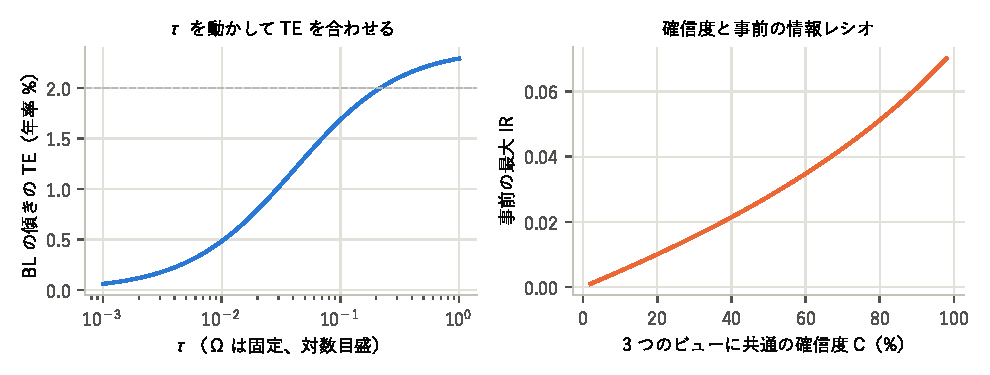
\includegraphics[width=0.95\linewidth]{fig_te.pdf}
\caption{Idzorek の例。左：$\Omega$ を固定して $\tau$ を動かしたときの、BL の傾きの TE。右：3 つのビューに共通の確信度 $C$（Idzorek の方法）と、事前の最大の IR。}
\label{fig:te}
\end{figure}

\figref{fig:te} の右のとおり、確信度を上げると事前の IR は上がる。確信度 50\% で \V{te.ir.c50}、90\% で \V{te.ir.c90} である。確信度を上げることは、TE を増やすだけでなく、「ずれ 1 単位あたりの見込み」も大きく見せる。$\tau$ で TE を合わせると、ずれの許容幅の都合で確信度を変えることになり、事前の IR が実力以上に大きく見えたり小さく見えたりする。この資料では、2 番目（$\Omega$ は当たり具合、TE は制約）を勧める。

\section{情報レシオの目安}

\begin{itemize}
\item Bevan と Winkelmann（1998）は、BL の比率の事前の IR が 2.0 を超えたら、ビューの重みを下げるよう勧めている（Idzorek による紹介）。
\item 実績の IR は、0.5 あれば優秀、1.0 なら例外的とされる。基本法則 $\IR\approx\IC\sqrt{\mathrm{BR}}$ で、IC 0.05 なら、独立な賭けが年に 100 回で IR 0.5 になる。
\item 事前の IR が 1 を大きく超えるなら、$\Omega$ が小さすぎる（ビューを信じすぎている）か、$\Omega$ を対角にして確信を積み上げている（\secref{sec:diag-trap}）可能性を疑う。
\end{itemize}

\section{本プロジェクトの TE}\label{sec:te-project}

\chapref{ch:project} で、本プロジェクトの LLM のビューを、較正した採用率で入れたうえで、事前の TE を年率 \V{bt.te.target}\% 以内にする制約を付けて最適化した。30 か月の実績の TE は \V{bt.fullte.te}\% で、目標を大きく上回った。制約を付けない場合の実績の TE は \V{bt.full.te}\% だったので、制約はずれを大きく減らしたが、目標どおりにはならなかった。

事前の TE が実績より小さく出るのは、次の理由による。

\begin{itemize}
\item 共分散は過去 252 日の縮小推定で、急な変動や個別の銘柄のニュースを捉えきれない。
\item 比率が毎月大きく入れ替わるので、月ごとに違う能動的な比率の TE を平均することになる。
\item 数百の銘柄に小さな比率を張ると、個別リスクの推定の誤差が積み上がる。
\end{itemize}

TE の制約を付けるときは、事前の目標を、実績が目標に収まるように控えめに置く（例えば実績の目標の半分程度）か、実績を見ながら調整する必要がある。

\begin{tipbox}[コツ：TE と IR]
\begin{enumerate}
\item ビューの中身（向き）と、ずれの大きさ（TE）は別々に決める。$\Omega$ は当たり具合で、TE は制約で。
\item 事前の IR が 1 を大きく超えたら、ビューを信じすぎていないか疑う。
\item TE だけで最適化すると、ベータや総リスクが増えることがある。ベータのずれと総リスクも確かめる。
\item 事前の TE は実績より小さく出やすい。実績の TE を見て、事前の目標を調整する。
\end{enumerate}
\end{tipbox}

\begin{keybox}[この章のまとめ]
\begin{itemize}
\item BL の結果は、時価総額の比率からの能動的な傾きで、その TE と IR で評価できる。
\item TE を罰則にした最適化の答えは、向き（$\alpha$ と $\Sigma$）と大きさ（TE の目標）に分かれる。最大の IR は $\alpha$ の大きさ、つまり $\Omega$ で決まる。
\item $\tau$ で TE を合わせると、確信度と許容幅を混ぜてしまう。$\Omega$ は当たり具合で、TE は制約で決めるのがよい。
\item 本プロジェクトでは、事前の TE を 3\% に制限しても、実績の TE は \V{bt.fullte.te}\% だった。
\end{itemize}
\end{keybox}


\part{本プロジェクトへの当てはめ}
% ============================================================
\chapter{本プロジェクトの LLM のビューで確かめる}\label{ch:project}

この章では、ここまでのコツを本プロジェクトのデータに当てはめる。LLM の予想の当たり具合を測り、回答のばらつきと実際の外れを比べ、$\Omega$ の決め方を 7 通りに変えて 30 か月の比率を計算し直す。

\section{データと設定}

\begin{itemize}
\item \textbf{LLM の回答}：実行番号 1（gpt-4o-mini、温度 1.0、1 銘柄あたり 30 回）。判断日は 2024 年 3 月 28 日〜2026 年 8 月 31 日の各月末の \V{llm.months} 回。各判断日の \SP{} の構成銘柄について、その月の日次リターンを渡し、翌月の日次の平均リターンを答えさせた。
\item \textbf{実際の結果}：判断日の翌月の日次リターンの平均（15 日以上のデータがある銘柄）。銘柄と月の組は \V{llm.rows} 個。
\item \textbf{BL}：本プロジェクトのコード（\code{blm/}）をそのまま使う。共分散は過去 252 取引日の縮小推定、$\delta=\V{blm.delta}$、$\tau=\V{blm.tau}$、$P=I$、最適化は空売りなし・全額投資。
\end{itemize}

\section{当たり具合}

\begin{table}[htbp]
\centering
\caption{判断日ごとの当たり具合。順位相関と相関は予想と翌月の実際の相関、傾き $b$ は実際を予想に回帰した傾き、入力との相関は予想と渡した月の平均リターンの相関、右端は回答の分散 ÷ 誤差の 2 乗の中央値。}
\label{tab:llm-monthly}
\small
\tabin{llm_monthly}
\end{table}

\begin{figure}[htbp]
\centering
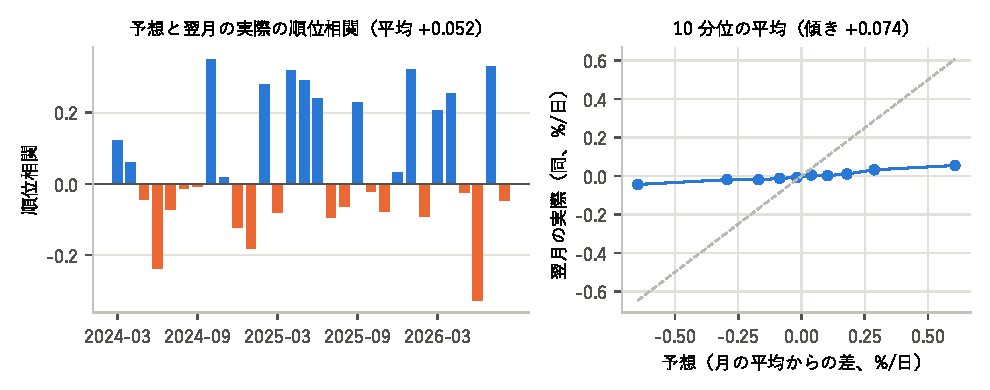
\includegraphics[width=0.95\linewidth]{fig_llm_ic.pdf}
\caption{左：判断日ごとの、予想と翌月の実際の順位相関。右：判断日ごとに平均を引いた予想の 10 分位ごとの、翌月の実際（同じく平均を引いたもの）。破線は 45 度の線。}
\label{fig:llm-ic}
\end{figure}

\tabref{tab:llm-monthly} と\figref{fig:llm-ic} から分かることを挙げる。

\begin{itemize}
\item 順位相関の平均は \V{llm.ic.mean}（$t$ 値 \V{llm.ic.t}、30 か月のうちプラスは \V{llm.ic.pos} か月）。相関（Pearson）の平均は \V{llm.icp.mean}。値としては、優れた運用者の目安（0.05 前後）と同じくらいだが、偶然と区別できるほどではない。
\item 傾き $b$ の平均は \V{llm.slope.mean}（$t$ 値 \V{llm.slope.t}）、30 か月をまとめると \V{llm.slope.pooled}。予想の散らばりのうち、翌月の差につながっているのは 7\% 程度である。\figref{fig:llm-ic} の右の 10 分位の点は、45 度の線よりずっと寝ている。
\item 予想と渡した月の平均リターンの相関は \V{llm.cin.mean}。予想は、ほぼ先月の値動きの写しである（『総合報告書』問題 2）。
\end{itemize}

予想の散らばり（判断日ごとの標準偏差の平均）は日次 \V{llm.sdQ}\%、実際の翌月の平均リターンの散らばりは \V{llm.sdr}\% で、大きさは近い。しかし、相関が 0.05 程度なので、予想を期待リターンとしてそのまま使うと、十数倍の自信過剰になる（傾き 0.07 の逆数は約 14）。

\section{回答のばらつきと、実際の外れ}

\begin{figure}[htbp]
\centering
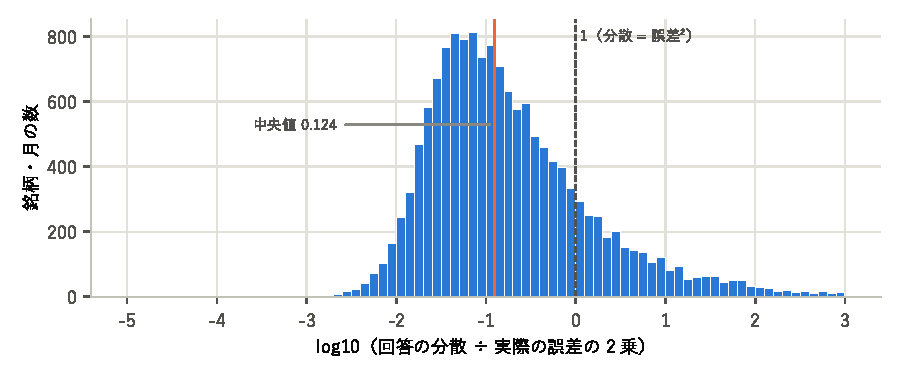
\includegraphics[width=0.92\linewidth]{fig_llm_ratio.pdf}
\caption{回答の分散 ÷ 実際の誤差の 2 乗（銘柄・月ごと、対数）。1（破線）なら、ばらつきが外れの大きさと合っている。}
\label{fig:llm-ratio}
\end{figure}

回答の分散と、実際の予想の外れ（予想 $-$ 翌月の実際）の 2 乗の比は、中央値で \V{llm.ratio.med}、四分位で \V{llm.ratio.q25}〜\V{llm.ratio.q75} だった（\figref{fig:llm-ratio}）。回答の標準偏差の中央値は日次 \V{llm.omsd}\% で、実際の外れ（誤差の 2 乗の平均の平方根で日次 0.6\% 前後）よりずっと小さい。

\chapref{ch:accuracy} の式~\eqref{eq:omega-err} で、避けられない外れ（翌月の日次リターンの平均そのものの散らばり）を差し引いても、外れの分散は回答の分散の平均の 5 倍以上だった。回答のばらつきを $\Omega$ にすると、外れを 5〜8 分の 1 に見積もることになる。

\section{1 銘柄で見た採用率}

回答の分散を、$\tau\Sigma$ の対角（$\tau=0.025$、過去 1 年の日次の分散）と比べると、比の中央値は \V{llm.omtau.med} で、1 銘柄だけで見た採用率は \V{llm.adopt.med}\% になる（\chapref{ch:overview} の\figref{fig:adoption}）。当たり具合から見た妥当な採用率（傾き 0.07 程度）の 10 倍以上である。

\section{$\Omega$ の決め方を変えて計算し直す}

$\Omega$ の決め方を次の 7 通りにして、30 か月の比率を計算し直した。

\begin{enumerate}
\item \textbf{回答の分散（元の方法）}：$\Omega=\diag(\text{回答の分散})$。本プロジェクトの「直した計算」と同じ。
\item \textbf{He--Litterman}：$\Omega=\tau\diag(\Sigma)$。1 銘柄なら採用率 50\%。
\item \textbf{傾きで較正（対角）}：$\Omega=\tau\diag(\Sigma)(1/b_t-1)$。1 銘柄なら採用率 $b_t$。
\item \textbf{傾きで較正（$\Sigma$ に比例）}：$\Omega=\tau\Sigma(1/b_t-1)$。どの銘柄も採用率 $b_t$ で、$\muBL=\Pi+b_t(Q-\Pi)$。
\item \textbf{同上 ＋ TE \V{bt.te.target}\% 以内}：4 と同じ期待リターンで、事前の TE を年率 \V{bt.te.target}\% 以内に制限する。
\item \textbf{相対ビュー ＋ TE \V{bt.te.target}\% 以内}：予想と均衡から、それぞれの時価総額加重の平均を引いた差だけを使い（$\muBL=\Pi+b_t[(Q-\wmkt\T Q)-(\Pi-\wmkt\T\Pi)]$）、5 と同じ TE の上限を置く。
\item \textbf{時価総額加重}：ベンチマーク。
\end{enumerate}

$b_t$ は、判断日 $t$ より前に結果が分かっている月だけで計算した傾き（月ごとに平均を引いてまとめる）で、0〜1 に収めた。最初の数か月はデータがなく、$b_t=0$（均衡のまま）である。30 か月のうち \V{bt.b.zero} か月が $b_t=0$ で、最後の判断日の $b_t$ は \V{bt.b.last} だった。

\begin{table}[htbp]
\centering
\caption{$\Omega$ の決め方と、30 か月の比率の性質と成績（年率 \%）。採用率は銘柄ごとの $(\muBL-\Pi)/(Q-\Pi)$ の中央値、実質銘柄数は $1/\sum w^2$ の平均、指数との差は $\frac12\sum|w-\wmkt|$ の平均、TE・IR は時価総額加重に対する実績、回転率は月平均。}
\label{tab:blm-omega}
\tabin{blm_omega}
\end{table}

\begin{figure}[htbp]
\centering
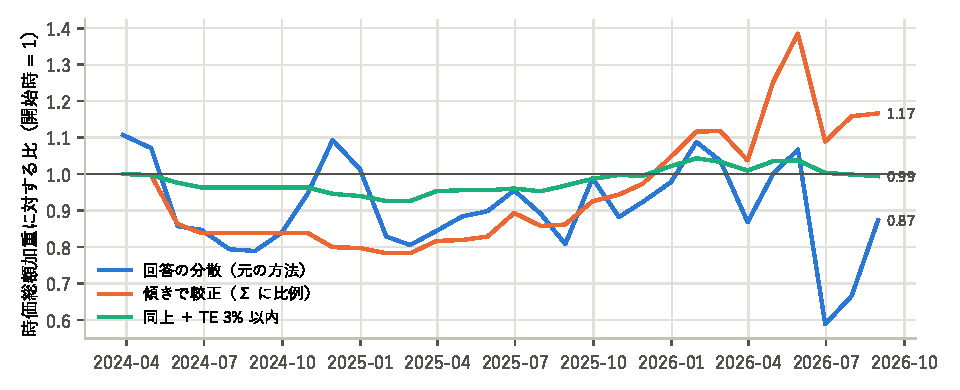
\includegraphics[width=0.95\linewidth]{fig_blm_omega.pdf}
\caption{時価総額加重に対する累積の比（30 か月）。}
\label{fig:blm-omega}
\end{figure}

\begin{figure}[htbp]
\centering
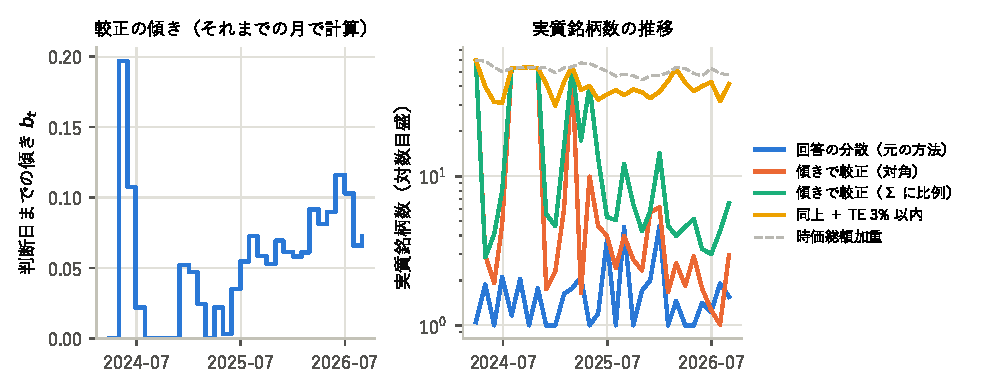
\includegraphics[width=0.98\linewidth]{fig_blm_omega_time.pdf}
\caption{左：判断日までに分かっている月だけで計算した較正の傾き $b_t$。右：比率の実質銘柄数の推移（対数目盛）。}
\label{fig:blm-omega-time}
\end{figure}

\figref{fig:blm-omega-time} の左のとおり、較正の傾き $b_t$ は、最初の 2 か月はデータがないので 0 である。結果が 1〜2 か月分しかない時期には 0.2 まで跳ね、その後しばらくは負の傾きを 0 に切り上げた 0 が続き、2025 年の半ば以降は 0.05〜0.12 の範囲に落ち着いた。少ない月から推定した傾きは大きく揺れるので、データが少ないうちは 0 に寄せて使うほうがよい（\secref{sec:slope}）。

右のとおり、回答の分散を $\Omega$ にした元の方法では、比率は毎月 1〜4 銘柄に集中する。較正した版は、$b_t=0$ の月には均衡のままなので時価総額加重と同じ比率（約 50 銘柄）になり、$b_t$ が正の月には、対角の $\Omega$ では数銘柄、$\Sigma$ に比例させても数銘柄〜十数銘柄に集中する。TE の上限を付けると、どの月も 30〜50 銘柄に収まる。採用率を正しく縮めても、TE の上限がなければ比率は集中する、ということが月ごとにも確かめられる。

\section{結果の読み方}

\tabref{tab:blm-omega} と\figref{fig:blm-omega} の読み方を、$\Omega$ の決め方ごとに述べる。

\begin{description}[leftmargin=2em,style=nextline]
\item[回答の分散・He--Litterman] 採用率は中央値で \V{bt.sample.adopt}\%、\V{bt.hl.adopt}\%。比率は実質 \V{bt.sample.effn}〜\V{bt.hl.effn} 銘柄に集中し、TE は年率 50\% 前後になった。BL というより、LLM の予想をそのまま期待リターンにした平均分散最適化で、成績は集中の結果である。He--Litterman の「ビューと均衡を半々」でも、約 490 銘柄を対角の $\Omega$ で入れると、採用率は 50\% を大きく超える。
\item[傾きで較正（対角）] 1 銘柄なら採用率 5〜7\% のはずが、中央値は \V{bt.calib.adopt}\% になった。約 490 個のビューの外れを独立と扱ったため、全体の水準（その月の予想の平均）への確信が積み上がった（\secref{sec:diag-trap}）。比率は実質 \V{bt.calib.effn} 銘柄、TE は \V{bt.calib.te}\% で、まだ大きい。
\item[傾きで較正（$\Sigma$ に比例）] 採用率は設定どおり \V{bt.full.adopt}\% になった。比率は実質 \V{bt.full.effn} 銘柄まで分散したが、TE は \V{bt.full.te}\% と、まだ大きい。期待リターンのずれが正しく縮められても、$\delta=2.5$ の平均分散最適化は、個別の銘柄に大きく賭ける。
\item[TE \V{bt.te.target}\% 以内] 比率は実質 \V{bt.fullte.effn} 銘柄で、時価総額加重（51.5 銘柄）に近づいた。年率リターンは \V{bt.fullte.ann}\%（時価総額加重は \V{bt.mkt.ann}\%）、リスクとシャープレシオも時価総額加重とほぼ同じになった。実績の TE は \V{bt.fullte.te}\% で、事前の目標を上回った（\secref{sec:te-project}）。
\item[相対ビュー ＋ TE] 結果は、5 の版とすべての指標で同じになった。$\Omega\propto\Sigma$ のもとでは、相対ビューとの違いは全銘柄の期待リターンへの一律の上乗せだけで、全額投資の制約があれば比率は変わらないからである（\chapref{ch:shape}）。採用率の列が \V{bt.relte.adopt}\% と小さく見えるのは、全体の水準の分を除いた差で測っているためである。全体の水準の癖が比率に効くのは、$\Omega$ が対角の場合（上の 1〜3）で、そこでは楽観・悲観が高ベータ・低ベータの銘柄への傾きとして現れる仕組みになっている。
\end{description}

\begin{notebox}[成績の差は偶然と区別できない]
30 か月の超過リターンの $t$ 値は、どの方法でも絶対値で 0.6 未満だった（較正・$\Sigma$ 比例で \V{bt.full.tstat}、TE 制約つきで \V{bt.fullte.tstat}）。この表から「どの方法が勝つか」は言えない。言えるのは、$\Omega$ の決め方で、採用率、集中、TE という比率の性質が大きく変わる、ということである。
\end{notebox}

\section{なぜ較正しても TE が大きいのか}

較正した採用率 5.6\% で、期待リターンのずれはどれくらいになるか。予想のずれ $Q-\Pi$ の散らばりは日次 0.35\% 程度（年率に直すと 80\% を超える）なので、5.6\% を掛けても年率で 5\% 前後のずれが残る。個別の銘柄の年率の特異リスクを 25\% とすると、制約のない最適化の能動的な比率は、1 銘柄あたりおおよそ $\alpha/(\delta\sigma^2)=0.05/(2.5\times0.0625)\approx30\%$ になる。数百の銘柄に、このような大きさの賭けが並べば、空売りなしの制約があっても TE は大きくなる。

つまり、$\delta=2.5$ は「市場全体のリスク」への回避度としては妥当でも、「ベンチマークからのずれ」への回避度としては小さすぎる。能動運用では、ずれへの回避度を別に（ずっと大きく）置くか、TE の上限を置く必要がある（\chapref{ch:te}）。

\section{限界}

\begin{itemize}
\item \textbf{期間が短い}：30 か月では、IC が 0.05 程度の予想の価値は確かめられない（\chapref{ch:accuracy} の推定の誤差）。
\item \textbf{モデルが 1 つ}：gpt-4o-mini だけである。対象論文のように複数のモデルで違う「スタイル」が出るかは、この比較では分からない。
\item \textbf{傾きの推定}：$b_t$ は少ない月から推定しており、最初の数か月は 0 だった。データがたまれば安定するが、それまでは 0 に寄せた値を使うのが安全である。
\item \textbf{取引費用}：この比較には入れていない。回転率は月 60〜100\% と大きく、費用を入れると成績はさらに下がる。
\item \textbf{先読み}：gpt-4o-mini の学習データの締め切り（2023 年 10 月）は、判断日（2024 年 3 月以降）より前である。ただし、構成銘柄の選び方などの先読みは『総合報告書』の議論のとおりで、ここでは扱っていない。
\end{itemize}

\section{本プロジェクトへの提案}

\begin{enumerate}
\item \textbf{較正の仕組みを組み込む}：DB には予想（\code{llm\_views}）と株価がそろっているので、判断日ごとに、それまでの月の傾き $b_t$（と IC）を計算して保存する。$\Omega$ はこの $b_t$ から決める。
\item \textbf{$\Omega$ を $\Sigma$ に比例させる}：$\Omega=\tau\Sigma(1/b_t-1)$ にすれば、事後の期待リターンは $\Pi+b_t(Q-\Pi)$ で、採用率が設定どおりになる。対角の $\Omega$ は使わない。
\item \textbf{相対ビューにする}：予想から判断日ごとの平均を引き、全体の水準の癖（楽観・悲観）を取り除く（\chapref{ch:shape}）。$\Omega\propto\Sigma$ と全額投資の組み合わせなら自動的に打ち消されるが、$\Omega$ を対角にする場合や、制約を変える場合に備えて、ビューの段階で取り除いておくのが安全である。
\item \textbf{TE の上限を置く}：事前の TE の上限を置く。実績が目標を上回るので、事前の目標は控えめにする。
\item \textbf{設定を変えたら較正し直す}：温度、質問、モデルを変えると、予想の散らばりも当たり具合も変わる。
\item \textbf{評価の指標}：成績（リターン）だけでなく、IC、傾き、回答の分散と誤差の比、採用率、実質銘柄数、TE を毎回記録する。
\end{enumerate}

\begin{keybox}[この章のまとめ]
\begin{itemize}
\item LLM の予想の当たり具合は、順位相関 \V{llm.ic.mean}、傾き \V{llm.slope.pooled} で、弱い正だった。
\item 回答の分散は、実際の外れの 2 乗の中央値の \V{llm.ratio.med} 倍で、予想を 8 倍前後信じすぎる設定になる。
\item $\Omega$ を傾きで較正し、$\Sigma$ に比例させると、採用率は設定どおり（\V{bt.full.adopt}\%）になった。対角のままだと \V{bt.calib.adopt}\% に積み上がった。
\item 較正しても、平均分散最適化は大きな TE を取る。TE の上限を置くと、比率は時価総額加重に近づいた。
\item 30 か月では、成績の差は偶然と区別できない。
\end{itemize}
\end{keybox}

% ============================================================
\chapter{LLM に聞くときの質問の設計}\label{ch:prompt}

BL のビューを LLM から作るとき、$\Omega$ の決め方だけでなく、LLM に「何を、どの形で聞くか」も結果を左右する。この章では、『総合報告書』の実験（D〜G）と先行研究の整理、この資料の結果をつなげて、BL に入れやすい質問の形をまとめる。

\section{本プロジェクトの実験で分かったこと}

『総合報告書』の実験の総合考察は、入力と質問の形を変えた 4 つの実験で、同じ性質がくり返し現れたとまとめている。

\begin{center}
\small
\begin{tabular}{p{0.9cm}p{5.0cm}p{7.0cm}}
\toprule
 & 変えたこと & 予想が沿っていたもの \\
\midrule
既存 & 1 か月分の日次リターンの列を渡す & 渡した月の平均リターン（相関 0.89） \\
D & 日次リターンを要約した指標に置き換え、財務の指標を足す & 直近 1 か月のリターン、12 か月のモメンタム \\
E & 考慮する比率を明言する & 直近 1 か月のリターン。値動きを 0\% にすると成長率 \\
F & 3 ターンの会話にし、答えを 5 段階にする & 直近 1 か月のリターン、または 12 か月のモメンタム（より強く） \\
G & 銘柄の数字を渡さず、リスクの種類ごとに聞く & 市場の直近 1 か月のリターンと VIX。セクターはセクターのモメンタム \\
\bottomrule
\end{tabular}
\end{center}

gpt-4o-mini は、渡された数字の中から「直近の値動き」に当たるものを見つけ、その向きに答える。ほかにも、次のことが分かっている。

\begin{itemize}
\item PER や ROE のような水準の指標は、どの条件でも予想に使われなかった。
\item 30 個の回答はそろいすぎていて、ばらつきは当たり具合を表さない。会話にするとさらにそろい、確率を直接読んでも 1 つの答えに集中する。
\item 銘柄の予想は 76\% がプラスで、リスクプレミアムはほぼ毎月「付く」と答える一方、セクターを指数と比べる問いでは 72\% が「指数より低い」と答えた。問いの形で偏りの向きが変わる。
\end{itemize}

先行研究も同じ方向の結果を示している（『総合報告書』の先行研究の章による）。Chen、Green、Gulen、Zhou（2024）は、LLM の株価の予想が直近の成績に重みを置きすぎ、楽観に偏ることを報告した。数値の時系列を LLM に予想させても良くならないという報告（Tan ほか 2024 など）がある一方、ニュースの見出しやニュースの判定のように、文章を読ませる使い方では成果が報告されている（Lopez-Lira and Tang、Anic ほか 2025）。財務諸表の分析で成果を報告した Kim, Muhn and Nikolaev（2024）は、2025 年 2 月に著者がデータと分析の不整合を理由に取り下げたので、根拠には使わない（2026 年 10 月 19 日に訂正）。

\section{BL の側から見た「良いビュー」}

ここまでの章の結果から、BL に入れやすいビューの条件をまとめる。

\begin{enumerate}
\item \textbf{当たり具合が測れる}：同じ形の予想を、同じ条件で、毎月記録できる。IC と較正の傾きが測れる（\chapref{ch:accuracy}）。
\item \textbf{全体の水準の癖を取り除ける}：楽観・悲観の偏りは全体の水準に出る。相対ビューにできる形がよい（\chapref{ch:shape}）。
\item \textbf{外れの相関が小さい}：銘柄ごとに独立な情報（銘柄ごとのニュースなど）に基づく予想は、外れが相関しにくい。同じ入力（市場の値動き）からすべての銘柄を予想すると、外れが共通になる（\chapref{ch:stacking}）。
\item \textbf{統計モデルにない情報を持つ}：直近の値動きのなぞりは、統計モデルで作れる（そして、この期間はほとんど当たっていない、\chapref{ch:esg}）。LLM を使う価値は、文章のような、統計モデルが扱いにくい情報にある。
\end{enumerate}

\section{聞き方の選択肢と、BL での扱い}

\begin{table}[htbp]
\centering
\caption{LLM への聞き方と、BL での扱い。}
\label{tab:prompt-forms}
\small
\begin{tabular}{p{2.3cm}p{3.2cm}p{3.4cm}p{3.4cm}}
\toprule
聞き方 & 例 & $Q$ の作り方 & $\Omega$ の作り方 \\
\midrule
数値 & 翌月の日次の平均リターン & 平均を引いて相対ビューにし、傾き $b$ で縮める & $\Omega\propto\Sigma$、採用率 $b$ \\
順位・区分 & セクター内の 5 分位、上位・下位 & 区分を点数 $z$ にし、$\IC\cdot\sigma\cdot z$ & 区分の IC から（市場版で $\omega=\sigma^2(1/\IC^2-1)$） \\
確率 & 強気・中立・弱気の確率 & 確率で重み付けた値（\chapref{ch:text}） & エントロピーで順番を付け、大きさは当たり具合で較正 \\
相対の差 & 「この銘柄はセクターを上回るか」 & 差のビュー（$P$ の行の和が 0） & 差の予想の当たり具合から \\
シナリオ & 「関税が上がったら、どのセクターが下がるか」 & 外部の変数へのビュー（\chapref{ch:politics}） & ストレステストとして控えめに（$c\le1$） \\
文章の判定 & 「このニュースはモメンタムの流れを支持するか」 & 統計のビューの採否・大きさの調整 & 判定の当たり具合から \\
\bottomrule
\end{tabular}
\end{table}

\tabref{tab:prompt-forms} のどの聞き方でも、$\Omega$ を LLM 自身に言わせることはしていない。LLM に確信の度合いを言わせると自信過剰になりやすい（Xiong ほか 2024）うえ、本プロジェクトでは回答のばらつきも当たり具合と合わなかった。確信の大きさは、記録した予想と結果から、こちらで測る。

\section{質問を作るときのコツ}

\begin{description}[leftmargin=2em,style=nextline]
\item[直近の値動きだけを渡さない] 渡せば、それをなぞる。値動きのビューが欲しいなら、LLM を通さず統計で作る。LLM には、値動きでは分からない情報（文章）を渡す。
\item[相対で聞く] 「上がるか」ではなく「セクター（や市場）を上回るか」と聞く。全体の水準の楽観・悲観が、答えに入りにくくなる。
\item[数値より順位や区分で聞く] 数値は桁が壊れやすく（実験 E）、単位の取り違えも起きる。区分なら、区分ごとの当たり具合を測って点数にすればよい。
\item[単位と形式をはっきりさせる] 数値で聞くなら、小数か百分率かを明記し、構造化した出力（JSON の形式など）にする。本プロジェクトの元のプロンプトは「percentage change」と書きながら小数を渡していた。
\item[温度と回数を固定し、記録する] 温度、回答の回数、プロンプトの版、モデルの版を、予想と一緒に保存する。どれかを変えたら、当たり具合を測り直す。回答を何回か取って平均するのは、$Q$ の雑音を減らすためで、$\Omega$ を作るためではない。
\item[予想の期間を考える] 1 か月先は、値動きの雑音が大きく、当たり具合が測りにくい。四半期や半年先のほうが、文章の情報が効く余地がある（その分、評価に時間がかかる）。
\item[未来の情報を混ぜない] モデルの知識の期限より後の期間で評価する。「過去の時点のつもりで答えて」という指示では、記憶からの答えを防げないという報告がある（『総合報告書』の先行研究の章）。
\item[複数のモデルは、外れの相関を測ってからまとめる] モデルを増やしても、同じ入力を見ている限り、外れは強く相関する（\chapref{ch:text}）。
\end{description}

\section{記録と評価の仕組み}

BL に LLM のビューを入れるなら、次の量を毎月記録し、一覧で見られるようにしておくとよい。

\begin{center}
\small
\begin{tabular}{p{4.0cm}p{9.6cm}}
\toprule
量 & 何を見るか \\
\midrule
IC（順位相関）と傾き $b$ & 予想が当たっているか。$b$ は採用率の材料 \\
入力との相関 & 予想が入力（直近の値動きなど）のなぞりになっていないか \\
予想の平均と実際の平均 & 全体の水準の癖（楽観・悲観）。相関が負なら全体の水準は入れない \\
回答の分散 ÷ 誤差の 2 乗 & 道具が出す不確かさが当たり具合と合っているか \\
外れの共通部分（$\rho_e$） & 対角の $\Omega$ が許されるか \\
採用率・実質銘柄数・TE & BL がどれだけ動いているか。成績の大部分はここで決まる \\
\bottomrule
\end{tabular}
\end{center}

本プロジェクトの DB には、予想（\code{llm\_views}）、株価、比率（\code{portfolio\_weights}）がそろっている。この表の量は、この資料の計算スクリプトの E、E2、S の節と同じ方法で、毎月計算できる。

\begin{keybox}[この章のまとめ]
\begin{itemize}
\item gpt-4o-mini は、渡された数字の中の直近の値動きをなぞる。予想は楽観に偏り、回答のばらつきは当たり具合を表さない。
\item BL に入れやすいのは、当たり具合が測れ、相対にでき、外れの相関が小さく、統計モデルにない情報を持つビューである。
\item 確信の大きさは LLM に言わせず、記録した予想と結果から測る。
\item 相対で、順位や区分で、単位をはっきりさせて聞き、設定を記録する。
\end{itemize}
\end{keybox}

% ============================================================
\chapter{ビューとリスクのコツ（一覧）}\label{ch:tips}

この章は、ここまでのコツを、使う順に並べたものである。各項目の末尾の括弧は、詳しく扱った章である。

\section{始める前に}

\begin{enumerate}[label=\textbf{\arabic*.},leftmargin=2.2em]
\item \textbf{採用率で考える。} BL の結果を決めるのは、$\Omega$ と $\tau\Sigma$ の比である。1 資産・1 ビューなら、均衡からビューへ動く割合は $s=\tau\sigma^2/(\tau\sigma^2+\omega)$。どの設定でも、まず $s$ がいくつになっているかを計算する（\ref{ch:overview}）。
\item \textbf{単位をそろえる。} $\Sigma$、$\Pi$、$Q$、$\Omega$ は、同じ期間（日次・月次・年率）の、同じ種類（超過リターン）の量で書く。無リスク金利の単位にも注意する（\ref{ch:prior}）。
\item \textbf{予想と結果の記録を残す。} $\Omega$ を決める唯一の確かな材料は、過去の予想と実際の結果の比較である。BL を動かす前から、記録を残す仕組みを作る（\ref{ch:accuracy}、\ref{ch:project}）。
\end{enumerate}

\section{事前分布（均衡・リスク回避度・共分散）}

\begin{enumerate}[label=\textbf{\arabic*.},leftmargin=2.2em,resume]
\item \textbf{均衡と最適化で同じ $\Sigma$ と $\delta$ を使う。} そうすれば、ビューがないときの比率は必ず時価総額の比率になる。ビューがないのに比率が動いていたら、どこかが食い違っている（\ref{ch:prior}）。
\item \textbf{$\delta$ は市場のリスクプレミアム ÷ 市場の分散。} 2.5〜3 程度がよく使われ、期間によらない（\ref{ch:prior}）。
\item \textbf{$\Sigma$ は推定できる形で作る。} 銘柄がデータの日数より多いなら、縮小推定かファクターモデルを使う。数週間のデータで数百銘柄の共分散を作らない（\ref{ch:prior}）。
\item \textbf{「市場」が何かを決める。} 時価総額の比率、浮動株調整後、ベンチマーク、等金額のどれを出発点にするかで、BL の意味が変わる（\ref{ch:prior}）。
\end{enumerate}

\section{$\tau$}

\begin{enumerate}[label=\textbf{\arabic*.},leftmargin=2.2em,resume]
\item \textbf{$\Omega$ が $\tau$ に比例するなら、$\tau$ は何でもよい。} He--Litterman や Idzorek の方法では、事後の期待リターンから $\tau$ が消える（\ref{ch:tau}）。
\item \textbf{$\Omega$ を外から決めるなら、$\tau$ は採用率の係数。} 回答の分散やモデルの分散を $\Omega$ にするなら、$\tau$ を変えると採用率が直接変わる。$\tau$ を決めることは、確信の度合いを決めることである（\ref{ch:tau}）。
\item \textbf{$\tau\approx1/T$ で大きさの感覚をつかむ。} 年率の $\Sigma$ で $\tau=0.025$ は、期待リターンの不確かさが年率で約 ±3\%（市場の標準偏差 20\% のとき）（\ref{ch:tau}）。
\item \textbf{少ない期間の成績で $\tau$ を選ばない。} 数か月の検証で $\tau$ を選ぶと、偶然に合わせてしまう（\ref{ch:tau}）。
\end{enumerate}

\section{ビューの値 $Q$}

\begin{enumerate}[label=\textbf{\arabic*.},leftmargin=2.2em,resume]
\item \textbf{ビューは均衡と比べて効く。} 言葉で「上回る」でも、均衡が示す差より小さければ、比率は逆に動く。$Q_k$ と $p_k\Pi$ を並べる（\ref{ch:idzorek}）。
\item \textbf{予想は当たり具合で縮める。} Grinold の式 $\alpha=\IC\cdot\sigma\cdot z$。生の予想の大きさのまま使うと、$1/\IC^2$ 倍の自信過剰になる（\ref{ch:accuracy}）。
\item \textbf{モデルの平均の式は、係数が有意か確かめる。} EGARCH-M のリスクの見返りのように有意でない係数で作ったビューは、危機のときに極端な値になる（\ref{ch:macro}）。
\item \textbf{順位しか信じられないなら、順位を点数に直す。} 正規分布の点数にして、順位の IC で大きさを決める（\ref{ch:shape}）。
\end{enumerate}

\section{ビューの不確かさ $\Omega$}

\begin{enumerate}[label=\textbf{\arabic*.},leftmargin=2.2em,resume]
\item \textbf{測れるなら測る。} 過去の記録があるなら、較正の傾き $b$（または $\IC^2$）を採用率にする。市場版なら $\omega=\sigma^2(1/\IC^2-1)$、元の BL なら $\omega=\tau\sigma^2(1/\IC^2-1)$（\ref{ch:accuracy}）。
\item \textbf{ビューが多いときは、$\Omega$ を対角にしない。} 外れの共通の部分を無視すると、ビューの数だけ確信が積み上がる。$\Omega\propto P\Sigma P\T$ にするか、共通の部分をビューから外す。本プロジェクトでは、対角の $\Omega$ で採用率が \V{bt.calib.adopt}\% に積み上がった（\ref{ch:omega}、\ref{ch:project}）。
\item \textbf{道具が出す不確かさは、そのまま使わない。} LLM の回答のばらつき、分布のエントロピー、モデルの予測分散は、外れやすさの順番の手がかりにはなりうるが、大きさは当たり具合で較正する。本プロジェクトでは、回答の分散は外れの約 8 分の 1 だった（\ref{ch:text}、\ref{ch:project}）。
\item \textbf{Idzorek の確信度は、ビュー 1 つのときの採用率。} 閉じた式 $\omega_k=\tau p_k\Sigma p_k\T(1-C_k)/C_k$ で計算できる。ビューが複数あると確信度どおりには動かない（\ref{ch:idzorek}）。
\item \textbf{言葉の確信度は、当たり具合と照らし合わせる。} 来月のリターンの予想なら、当たり具合に見合う確信度は 1\% 前後で、言葉で選ぶ 25〜65\% より 2 桁小さい（\ref{ch:idzorek}、\ref{ch:accuracy}）。
\item \textbf{ボラティリティで $\Omega$ を動かすなら、$\Sigma$ との速さの違いに注意する。} $\Omega$ だけを速く動かすと、危機の直後にビューをいちばん強く信じることになる（\ref{ch:macro}）。
\item \textbf{複数の予想をまとめるときは、外れの相関を考える。} 同じ実現値と比べる予想の外れは強く相関する。独立を仮定した精度加重は確信を過大にする（\ref{ch:text}）。
\end{enumerate}

\section{ビューの形}

\begin{enumerate}[label=\textbf{\arabic*.},leftmargin=2.2em,resume]
\item \textbf{全体の水準と銘柄間の差を分ける。} LLM の楽観・悲観の癖は全体の水準の部分である。銘柄間の差は相対ビューに、全体の水準は市場への 1 つのビューにする。$\Omega$ が対角だと、全体の水準の癖は高ベータ・低ベータの銘柄への傾きとして比率に入り込む（\ref{ch:shape}、\ref{ch:project}）。
\item \textbf{相対ビューの重みは時価総額で付ける。} 等しい重みは小さい資産を大きく動かす（\ref{ch:idzorek}）。
\item \textbf{資産が多いなら、ファクターへのビューを考える。} 数が少なく、相関が自然に入り、当たり具合も長いデータで測れる。ただし、事前分布を全データで信じすぎると、ビューはほとんど効かない（\ref{ch:shape}、\ref{ch:esg}）。
\item \textbf{外部の変数へのビューは、シナリオとして使う。} 地政学リスクやマクロの変数への条件付けは、市場版の BL で計算できる。ストレステストとして使い、確実なビューとしては入れない（\ref{ch:politics}）。
\end{enumerate}

\section{ファクターごとの注意}

\begin{enumerate}[label=\textbf{\arabic*.},leftmargin=2.2em,resume]
\item \textbf{政治：} 指数そのものより、シナリオと長い期間の不確かさに使う。短い期間の不確かさは、市場のボラティリティ（直近の実現値、VIX）のほうが強い（\ref{ch:politics}）。
\item \textbf{テキスト・LLM：} 成績の数字は、期間・銘柄の数・費用・$\Omega$ の大きさを確かめてから読む。温度や質問を変えたら較正し直す（\ref{ch:text}）。
\item \textbf{マクロ：} 景気の局面のビューは、局面の数の少なさと、判定の先読みに注意する（\ref{ch:macro}）。
\item \textbf{財務・ESG：} 指標は IC を測ってから点数にする。ESG を共分散で表すなら、均衡と最適化のどちらに入れるかを決める。両方に入れると効かず、$\Omega$ を固定していると低 ESG の銘柄のビューを強く信じる方向に働く（\ref{ch:esg}）。
\item \textbf{モメンタム：} 12--1 か月で順位を付け、モメンタム自身のボラティリティが高いときは確信度を下げる。直近 1 か月の写しは、個別株の短期の反転と逆の向きの賭けである（\ref{ch:momentum}）。
\end{enumerate}

\section{最適化}

\begin{enumerate}[label=\textbf{\arabic*.},leftmargin=2.2em,resume]
\item \textbf{ビューの中身と、ずれの大きさを分ける。} $\Omega$ は当たり具合で、TE は制約で決める。$\tau$ で TE を合わせない（\ref{ch:te}）。
\item \textbf{能動運用では TE の上限を置く。} 正しく縮めた期待リターンでも、$\delta=2.5$ の平均分散最適化は個別の銘柄に大きく賭ける（\ref{ch:project}）。
\item \textbf{事前の TE は実績より小さく出る。} 実績を見て、事前の目標を調整する（\ref{ch:te}、\ref{ch:project}）。
\item \textbf{TE だけで最適化すると、ベータと総リスクが増えることがある。} ベータのずれと総リスクも確かめる（\ref{ch:te}）。
\item \textbf{裾のリスクを気にするなら、期待リターンは BL、リスクは裾の厚いシナリオで。} 楕円分布なら CVaR は分散と同じ答えになる（\ref{ch:cvar}）。
\item \textbf{平均以外のビューは、エントロピー・プーリングで。} 順位、ボラティリティ、下落の確率、相関のビューを入れられる。平均だけなら BL で十分（\ref{ch:ep}）。
\end{enumerate}

\section{確かめ方}

\begin{enumerate}[label=\textbf{\arabic*.},leftmargin=2.2em,resume]
\item \textbf{黙示の確信度を計算する。} 100\% 信じたときの傾きに対して、実際に何割傾いたかを見る（\ref{ch:idzorek}）。
\item \textbf{事前の IR が 1 を大きく超えたら疑う。} ビューを信じすぎているか、対角の $\Omega$ で確信を積み上げている（\ref{ch:te}）。
\item \textbf{比率の性質を記録する。} 採用率、実質銘柄数、指数との差、TE、回転率を毎回記録する。成績だけで方法を選ばない（\ref{ch:project}）。
\item \textbf{成績の差の $t$ 値を見る。} 数年分の月次データでは、IC 0.05 程度の予想の価値は確かめられない（\ref{ch:accuracy}、\ref{ch:project}）。
\end{enumerate}

% ============================================================
\chapter{まとめ}\label{ch:summary}

この資料は、Black-Litterman モデルのビュー $Q$、その不確かさ $\Omega$、均衡の不確かさ $\tau$ の決め方を、論文を読んで整理し、本プロジェクトのデータと論文の数値例で確かめた。

\section{分かったこと}

\begin{description}[leftmargin=2em,style=nextline]
\item[1. BL の結果は採用率で決まる] 均衡からビューへ何割動くかは、$\Omega$ と $\tau\Sigma$ の比で決まる。He--Litterman の既定値では 50\%、予想の当たり具合に合わせると IC の 2 乗（多くは 1\% 未満）で、この違いが BL の結果の違いの大部分を生む。$\Omega$ を $\tau$ に比例させれば $\tau$ は消え、$\Omega$ を外から決めれば $\tau$ が採用率の係数になる。
\item[2. 確信度の方法は閉じた式になる] Idzorek の 8 資産の例は論文の表どおりに再現でき、確信度の方法は $\omega_k=\tau p_k\Sigma p_k\T(1-C_k)/C_k$ と同じだった。確信度は 1 つのビューの採用率で、ビューが複数あると相関によって確信度どおりには動かない。
\item[3. 当たり具合から $\Omega$ を決めると、Grinold の式になる] 市場版の BL で $\omega=\sigma^2(1/\IC^2-1)$ と置くと、事後の期待リターンは $\IC\cdot\sigma\cdot z$ に一致する。BL は、昔からの「予想を当たり具合で縮める」実務と同じものである。
\item[4. 対角の $\Omega$ は確信を積み上げる] 同じ情報源から多くのビューを作ると、外れには共通の部分がある。$\Omega$ を対角にすると、それを無視して、ビューの数だけ確信が積み上がる。本プロジェクトのデータで、1 銘柄なら 5〜7\% の採用率が、対角の $\Omega$ では中央値 \V{bt.calib.adopt}\% になった。
\item[5. 道具が出す不確かさは、当たり具合と合わない] LLM の回答のばらつきは、実際の外れの約 8 分の 1 だった。調査メモの「ばらつきが不確かさを客観的に表す」という主張は、本プロジェクトのデータでは成り立たない。
\item[6. ファクターごとの材料は、使い方を選ぶ] 政治の指数は、短い期間の不確かさでは市場のボラティリティに及ばず、シナリオや長い期間の見込みに向く。マクロのモデルの平均の式は危機で極端になりうる。ESG を共分散に入れる案は、入れ方によって効かないか、意図と逆に働く。モメンタムは、自身のボラティリティで確信度を下げると急落を和らげられる。
\item[7. 拡張は、平均以外のビューと裾のリスクのため] エントロピー・プーリングは、平均のビューなら BL とほぼ同じ答えを出し、順位・ボラティリティ・下落の確率のビューも入れられる。CVaR は、楕円分布に近い資産では分散と同じ答えになる。
\item[8. 最適化ではずれの大きさを別に決める] 正しく縮めた期待リターンでも、平均分散最適化は大きなトラッキングエラーを取る。$\Omega$ は当たり具合で、TE は制約で決める。事前の TE は実績より小さく出やすい。
\end{description}

\section{本プロジェクトへの示唆}

本プロジェクトの BL は、いまは LLM の回答の分散を $\Omega$ にしており、採用率が非常に高く、比率は少数の銘柄に集中する。この資料の結果から、次の順に直すのがよいと考える（\chapref{ch:project}）。

\begin{enumerate}
\item 予想と結果から、判断日ごとに較正の傾き $b_t$ を計算する。
\item $\Omega=\tau\Sigma(1/b_t-1)$ とし、採用率を $b_t$ にそろえる。
\item 予想から判断日ごとの平均を引き、相対ビューにする。
\item 事前の TE に上限を置き、実績の TE を見て調整する。
\item 採用率、実質銘柄数、TE、IC を毎回記録し、成績だけで方法を選ばない。
\end{enumerate}

これらは、LLM の予想が「当たるかどうか」を判断する前に必要な、測り方の整備である。予想の価値（IC が本当に 0 より大きいか）は、記録をためて確かめるしかない。BL は、価値の分からない予想を、分からない程度に応じて控えめに使う仕組みとして働かせるのがよい。

\section{残った問い}

\begin{itemize}
\item LLM の予想の当たり具合は、局面（上昇相場・下落相場、ボラティリティの高さ）でどう変わるか。変わるなら、$\Omega$ をどう動かすべきか。
\item 複数の LLM の予想の外れは、どれくらい相関しているか。融合で本当に改善するか。
\item セクターやファクターのような、数の少ないビューにしたとき、LLM の予想の当たり具合は上がるか。
\item 文章の情報（月次レポート、決算説明会）を加えたとき、IC は上がるか。
\end{itemize}

どの問いも、この資料で示した測り方（IC、較正の傾き、外れと不確かさの比、採用率、TE）で答えられる。


\appendix
% ============================================================
\chapter{行列の公式と導出}\label{app:formulas}

本文で使った公式と、省いた導出をまとめる。

\section{平方完成}

対称で正定値の行列 $H$ とベクトル $h$ について、
\begin{equation}
-\tfrac12\mu\T H\mu+\mu\T h=-\tfrac12(\mu-H^{-1}h)\T H(\mu-H^{-1}h)+\tfrac12h\T H^{-1}h
\end{equation}
が成り立つ。右辺を展開すれば確かめられる。密度が $\exp(-\frac12\mu\T H\mu+\mu\T h)$ に比例する分布は、平均 $H^{-1}h$、共分散 $H^{-1}$ の正規分布である。

\section{Woodbury の公式}

正則な $A$（$n\times n$）、$C$（$k\times k$）と、$U$（$n\times k$）、$V$（$k\times n$）について、
\begin{equation}
(A+UCV)^{-1}=A^{-1}-A^{-1}U\bigl(C^{-1}+VA^{-1}U\bigr)^{-1}VA^{-1}
\end{equation}
が成り立つ。

\subsection*{情報形から更新形へ}

$A=(\tau\Sigma)^{-1}$、$U=P\T$、$C=\Omega^{-1}$、$V=P$ とすると、事後の共分散は
\begin{equation}
M=\bigl[(\tau\Sigma)^{-1}+P\T\Omega^{-1}P\bigr]^{-1}=\tau\Sigma-\tau\Sigma P\T\bigl(\Omega+P\tau\Sigma P\T\bigr)^{-1}P\tau\Sigma
\end{equation}
である。事後の平均 $\muBL=M\bigl[(\tau\Sigma)^{-1}\Pi+P\T\Omega^{-1}Q\bigr]$ に代入する。$K=P\tau\Sigma P\T+\Omega$ と書くと、
\begin{align}
M(\tau\Sigma)^{-1}\Pi&=\Pi-\tau\Sigma P\T K^{-1}P\Pi,\\
MP\T\Omega^{-1}Q&=\tau\Sigma P\T\Omega^{-1}Q-\tau\Sigma P\T K^{-1}P\tau\Sigma P\T\Omega^{-1}Q\notag\\
&=\tau\Sigma P\T K^{-1}\bigl(K-P\tau\Sigma P\T\bigr)\Omega^{-1}Q=\tau\Sigma P\T K^{-1}Q
\end{align}
となり、足すと更新形 $\muBL=\Pi+\tau\Sigma P\T K^{-1}(Q-P\Pi)$ が得られる。

\section{正規分布の条件付き分布}

$(x,y)$ が同時に正規分布に従い、
\begin{equation}
\begin{pmatrix}x\\y\end{pmatrix}\sim\mathcal N\left(\begin{pmatrix}m_x\\m_y\end{pmatrix},
\begin{pmatrix}S_{xx}&S_{xy}\\S_{yx}&S_{yy}\end{pmatrix}\right)
\end{equation}
なら、$y$ を観測したときの $x$ は
\begin{equation}
x\mid y\sim\mathcal N\bigl(m_x+S_{xy}S_{yy}^{-1}(y-m_y),\;S_{xx}-S_{xy}S_{yy}^{-1}S_{yx}\bigr)
\end{equation}
に従う。

\subsection*{市場版の BL}

$x\sim\mathcal N(\pi,\Sigma)$、$v=Px+\varepsilon$、$\varepsilon\sim\mathcal N(0,\Omega)$（$x$ と独立）なら、$\Cov(x,v)=\Sigma P\T$、$\Var(v)=P\Sigma P\T+\Omega$ なので、上の公式から
\begin{equation}
x\mid v\sim\mathcal N\bigl(\pi+\Sigma P\T(P\Sigma P\T+\Omega)^{-1}(v-P\pi),\;\Sigma-\Sigma P\T(P\Sigma P\T+\Omega)^{-1}P\Sigma\bigr)
\end{equation}
が得られる（式~\eqref{eq:mbl-mu}、\eqref{eq:mbl-sigma}）。元の BL は、$x$ を $\mu$ に、$\Sigma$ を $\tau\Sigma$ に置き換えたものである。

\subsection*{外部の変数への条件付け}

資産のリターン $X$ と外部の変数 $g$ の同時分布で、$g=v$ を条件にすると、$\E[X\mid g=v]=\pi_X+\Sigma_{Xg}\Sigma_{gg}^{-1}(v-\pi_g)$ である。$\Sigma_{Xg}\Sigma_{gg}^{-1}$ は、$X$ を $g$ に回帰したときの係数である。不確かさ $\Omega$ を付けるなら、$\Sigma_{gg}$ を $\Sigma_{gg}+\Omega$ に置き換える。

\section{1 つのビューの傾きの比}

1 つのビュー $p$（行ベクトル）について、制約のない最適化の傾きは、式~\eqref{eq:hl-weights} から
\begin{equation}
w(\omega)-\wmkt=p\T\,\frac{\tau}{\delta}\cdot\frac{Q-p\Pi}{\tau p\Sigma p\T+\omega}
\end{equation}
である。$\omega=0$ のときとの比は $\tau p\Sigma p\T/(\tau p\Sigma p\T+\omega)$ で、資産によらない。これを確信度 $C$ に等しくおけば、Idzorek の閉じた式 $\omega=\tau p\Sigma p\T(1-C)/C$ が得られる。

\section{較正の傾きと IC}

予想 $q$ と実際 $r$ の相関を $\IC$、標準偏差を $\sigma_q$、$\sigma_r$ とすると、実際を予想に回帰した傾きは
\begin{equation}
b=\frac{\Cov(q,r)}{\Var(q)}=\IC\cdot\frac{\sigma_r}{\sigma_q}
\end{equation}
である。$q=r+\varepsilon$（実際に雑音が乗ったもの）なら $\sigma_q^2=\sigma_r^2+\omega$、$\IC=\sigma_r/\sigma_q$ なので、$b=\IC^2=\sigma_r^2/(\sigma_r^2+\omega)$ になる。

\section{エントロピー・プーリングの双対}

条件を $Aq=b$（等式、$\one\T q=1$ を含む）と $Gq\le g$（不等式）とする。ラグランジュ関数
\begin{equation}
L(q,\lambda,\nu)=\sum_jq_j(\log q_j-\log p_j)+\lambda\T(Aq-b)+\nu\T(Gq-g),\qquad\nu\ge0
\end{equation}
を $q_j$ で微分して 0 とおくと、$q_j=p_j\exp(-1-a_j\T\lambda-g_j\T\nu)$（$a_j$、$g_j$ は $A$、$G$ の $j$ 列目）。これを戻した双対の関数
\begin{equation}
D(\lambda,\nu)=-\sum_jq_j(\lambda,\nu)-\lambda\T b-\nu\T g
\end{equation}
を、$\nu\ge0$ の範囲で最大にする。$-D$ は凸で、勾配は $(b-Aq,\ g-Gq)$ である。この資料の計算では、条件の行を標準化してから、準ニュートン法（L-BFGS-B）で解いた。

\section{線形の制約つきの能動運用の最適化}

能動的な比率 $w_a$ に線形の制約 $Bw_a=0$（$B$ は $m\times N$。例えば $\one\T$ と $(\Sigma w_b)\T$）を付けて、
\begin{equation}
\max_{w_a}\;w_a\T\alpha-\frac{\lambda_A}{2}w_a\T\Sigma w_a\quad\text{s.t.}\quad Bw_a=0
\end{equation}
を解く。ラグランジュ乗数 $\eta$ を使うと、$\alpha-\lambda_A\Sigma w_a-B\T\eta=0$ から $w_a=\frac{1}{\lambda_A}\Sigma^{-1}(\alpha-B\T\eta)$。制約に代入して $\eta=(B\Sigma^{-1}B\T)^{-1}B\Sigma^{-1}\alpha$ なので、
\begin{equation}
w_a^*=\frac{1}{\lambda_A}h,\qquad h=\Sigma^{-1}\alpha-\Sigma^{-1}B\T(B\Sigma^{-1}B\T)^{-1}B\Sigma^{-1}\alpha
\end{equation}
である。$h\T\Sigma h=h\T\alpha=\alpha\T\Sigma^{-1}\alpha-c\T(B\Sigma^{-1}B\T)^{-1}c$（$c=B\Sigma^{-1}\alpha$）で、これが最大の情報レシオの 2 乗になる。$B=\one\T$ なら本文の式~\eqref{eq:ir-star} である。

\section{CVaR の最小化の式}

$F(\zeta)=\zeta+\frac{1}{1-\beta}\E[(L-\zeta)^+]$ を $\zeta$ で微分すると、$1-\frac{1}{1-\beta}\Pr(L>\zeta)$ である。これが 0 になるのは $\Pr(L>\zeta)=1-\beta$、つまり $\zeta=\VaR_\beta$ のときで、そのときの値は
\begin{equation}
\VaR_\beta+\frac{1}{1-\beta}\E[(L-\VaR_\beta)^+]=\E[L\mid L\ge\VaR_\beta]=\CVaR_\beta
\end{equation}
である（連続な分布の場合）。$F$ は $\zeta$ と $w$ について凸なので、$\zeta$ と $w$ を一緒に最小化すればよい。シナリオで期待値を書けば、本文の線形計画~\eqref{eq:ru-lp} になる。

% ============================================================
\chapter{調査メモの主張の確認表}\label{app:check}

依頼のときに渡された調査メモの主な主張を、この資料で確かめた結果とともに並べる。「確認」は論文の本文または要旨で確かめられたもの、「一部」は内容の一部が違うか条件付きのもの、「未確認」は出典を見つけられなかったもの、「不成立」は本プロジェクトのデータで成り立たなかったものである。

\begin{longtable}{p{5.2cm}p{1.2cm}p{6.8cm}}
\toprule
調査メモの主張 & 結果 & 確かめた内容 \\
\midrule
\endfirsthead
\toprule
調査メモの主張 & 結果 & 確かめた内容 \\
\midrule
\endhead
\bottomrule
\endfoot
BL は Black と Litterman が 1990 年代に開発し、均衡（事前）とビューをベイズの枠組みで合成する & 確認 & Black and Litterman（1990、1991、1992）。BL の「ベイズ」が標準のベイズ推定と違う点は Meucci（2010）（\chapref{ch:derive}） \\
リスク回避度は市場のリスクプレミアム ÷ 市場の分散。プレミアム 3\% で 3.07 や 2.65 & 一部 & 3.07 は Idzorek の例のとおり（逆算で \V{idz.lam}）。2.65 の出典は確認できなかった（\chapref{ch:prior}） \\
Walters（2011）によれば、$\tau$ は 0.01〜0.10 程度、場合によっては $1/T$ & 一部 & Walters の本文は確認できなかった。0.01〜0.05（Lee 2000）は Idzorek の紹介、$1/T$ は Blamont and Firoozye と Meucci（\chapref{ch:tau}） \\
Kolm and Ritter（2021）がリスクファクターに拡張した枠組み & 一部 & APT のファクターのプレミアムへのビューを詳しく扱ったのは Kolm and Ritter（2017、EJOR）。2021 年は Kolm, Ritter and Simonian のサーベイ（\chapref{ch:shape}） \\
GPR は 10 紙の記事から脅威と行動を区別して作る & 確認 & Caldara and Iacoviello（2022）。8 区分のうち 5 つが脅威、3 つが行動（\chapref{ch:politics}） \\
GPRT は $\Omega$ を大きくする合図、GPRA は防衛・エネルギーへの方向のビュー & 未確認 & 論文にこの対応はない。調査メモの提案として扱った。データでは指数自体の説明力が弱かった（\chapref{ch:politics}） \\
EPU はニュースの頻度から政策の不確実性を数値化する & 確認 & Baker, Bloom and Davis（2016）。12,000 本の記事の監査（\chapref{ch:politics}） \\
Hassan ほか（2019）の手法で、約 7,000 社・24 万件超の決算説明会から企業ごとの GPR センチメントを取り出し、航空・運輸が負、防衛が恩恵 & 未確認 & Hassan ほか（2019）は企業ごとの政治リスクを測る論文で、NBER の版では 9,478 社・175,797 回（2002〜2016 年）。調査メモの数字と業種の結果は確認できなかった（\chapref{ch:politics}） \\
Sun ほか（2026）：BERT・LSTM の予想を BL に入れ、年率 106.58\%、シャープ 2.64、ソルティノ 4.18 & 確認（条件付き） & 数字は論文どおり。8 銘柄、117 取引日、$\Omega$ は単位行列と記載（\chapref{ch:text}） \\
LLM に 100 回聞き、平均を $Q$、分散を $\Omega$ にする & 確認 & 対象論文の第 2 版（第 1 版と本プロジェクトは 30 回）（\chapref{ch:text}） \\
LLM の出力のばらつきが情報の不確かさを直接表し、確信度を客観的に導出できる & 不成立 & 本プロジェクトのデータで、回答の分散は実際の外れの 2 乗の中央値の \V{llm.ratio.med} 倍（\chapref{ch:project}） \\
Beach and Orlov（2007）：EGARCH-M でビューを作る & 確認 & 要旨の範囲で確認（\chapref{ch:macro}） \\
同論文の平均の式（マクロ変数を含む）、条件付き分散を $\Omega$ にすること、$\tau=0.005$ と $0.01$ & 未確認 & 本文を確認できなかった \\
条件付き分散を $\Omega$ にすると、ボラティリティの急上昇で自動的に均衡へ戻る「自己修復」 & 一部 & 危機の始まりでは働くが、$\Sigma$ を長い期間で推定していると、危機の直後に採用率が \V{eg.adopt.max}\% まで上がる（\chapref{ch:macro}） \\
CVaR-BL-MCV で年金のシャープレシオが平均 19.7\% 改善 & 未確認 & 出典を見つけられなかった。近い研究は Sun, Wu and De（2023）の TVC-BL（10.5〜13.0\%）（\chapref{ch:macro}） \\
Fama--French の回帰の結果をビューにする & 確認（一般論） & 特定の論文は確かめていない。ファクターへのビューは Kolm and Ritter（2017）など（\chapref{ch:esg}） \\
ESG の点数で共分散を $(2-\mathrm{ESG})$ 倍に膨らませる（Ledoit--Wolf の推定に適用） & 未確認 & 出典を見つけられなかった。均衡と最適化に同じ共分散を使うと効かない。$\Omega$ を固定していると低 ESG のビューを強く信じる方向に働く（\chapref{ch:esg}） \\
ESG を共分散のペナルティにすると、ビューや事前分布と競合せずに ESG を統合できる & 一部 & 均衡を作り直すかどうかで結果が変わり、ビューの採用率にも影響する（\chapref{ch:esg}） \\
エントロピー・プーリングは相対エントロピーを最小化して、事前から事後へ確率を更新する & 確認 & Meucci（2008）。平均のビューなら BL とほぼ同じ答え（\chapref{ch:ep}） \\
確信度 $c$ で事前とビューを満たす分布を混ぜる & 確認 & Meucci のオピニオン・プーリング（\chapref{ch:ep}） \\
Meucci（2006）と近年の研究はコピュラ（$t$、vine）で暴落時の非対称な依存を表す & 一部 & Meucci（2006）は COP。vine コピュラと CVaR を BL と組み合わせたのは Teplova ほか（2023）（\chapref{ch:cop}） \\
Idzorek の確信度の方法で 0〜100\% の確信度から $\Omega$ を逆算する & 確認 & 閉じた式と一致。ビューが複数あると確信度どおりには動かない（\chapref{ch:idzorek}） \\
Walters（2014）：$\tau$ は 0.01〜0.05 程度に小さくすべき & 未確認 & Walters の本文を確認できなかった \\
トラッキングエラーの罰則つきの最適化で、極端な空売りや集中を避けつつビューを反映できる & 一部 & 能動運用の最適化は標準的。ただし、BL で縮めても平均分散最適化は大きな TE を取りうる。TE だけで最適化するとベータが増えうる（Roll 1992）（\chapref{ch:te}、\chapref{ch:project}） \\
\end{longtable}

% ============================================================
\chapter{論文の一覧}\label{app:papers}

この資料で扱った主な論文を、ビュー $Q$ と不確かさ $\Omega$ の作り方の観点で一覧にする。「確認」の列は、この資料で読んだ範囲（本文、要旨、ほかの文献での紹介）である。

\begin{longtable}{p{2.8cm}p{3.7cm}p{4.0cm}p{0.9cm}p{0.8cm}}
\toprule
論文 & $Q$ の作り方 & $\Omega$・$\tau$ の作り方 & 章 & 確認 \\
\midrule
\endfirsthead
\toprule
論文 & $Q$ の作り方 & $\Omega$・$\tau$ の作り方 & 章 & 確認 \\
\midrule
\endhead
\bottomrule
\endfoot
\multicolumn{5}{l}{\textbf{BL の基礎と $\Omega$・$\tau$}}\\
Black and Litterman（1992） & 投資家のビュー & $\tau$ は 0 に近い値 & \ref{ch:overview} & 紹介 \\
He and Litterman（1999） & 例のビュー & $\Omega=\tau\diag(P\Sigma P\T)$、$\tau=0.05$ & \ref{ch:hlmeucci} & 本文\textsuperscript{*} \\
Satchell and Scowcroft（2000） & 相対ビューは等しい重み & $\tau=1$ がよく使われる。$\tau$ を確率変数にするモデル & \ref{ch:tau} & 紹介 \\
Idzorek（2007） & 8 資産の 3 つのビュー、時価総額の重み & 確信度 0〜100\% から逆算 & \ref{ch:idzorek} & 本文 \\
Walters（2014） & --- & Idzorek の方法の閉じた式、$\tau$ の整理 & \ref{ch:tau} & 紹介 \\
Meucci（2010） & 言葉のビューを $\eta\sqrt{P\Sigma P\T}$ で数字に & $\Omega=\frac1cP\Sigma P\T$、市場版の BL（$\tau$ なし） & \ref{ch:hlmeucci} & 本文 \\
Kolm and Ritter（2017） & ファクターのプレミアムへのビュー（APT） & ベイズ回帰との対応、仮定の整理 & \ref{ch:derive}、\ref{ch:shape} & 紹介 \\
Spears, Zohren and Roberts（2023） & 機械学習の予想（BL--APT） & 予想モデルの不確かさ、複数のビューの融合 & \ref{ch:text} & 本文 \\
O'Toole（2017）、Allaj（2013） & --- & $\tau$ をアクティブリスクで決める、回帰で推定する & \ref{ch:tau} & 紹介 \\
\multicolumn{5}{l}{\textbf{政治・テキスト・LLM}}\\
Caldara and Iacoviello（2022） & 地政学リスク指数 & --- & \ref{ch:politics} & 本文 \\
Baker, Bloom and Davis（2016） & 経済政策不確実性指数 & --- & \ref{ch:politics} & 本文 \\
Hassan ほか（2019） & 企業ごとの政治リスク & --- & \ref{ch:politics} & 本文\textsuperscript{†} \\
Han and Li（2023） & --- & GEPU に基づくボラティリティ（GARCH-MIDAS）をビューの不確かさに & \ref{ch:politics} & 要旨 \\
Colasanto ほか（2022） & FT の記事のセンチメント → 価格のシミュレーション & --- & \ref{ch:text} & 要旨 \\
Sun, Fu and Liu（2026） & 掲示板のセンチメント → LSTM & 単位行列と記載 & \ref{ch:text} & 本文 \\
Mantshimuli and Muteba Mwamba（2025） & 3 つの LLM のセンチメントを LSTM でまとめる & --- & \ref{ch:text} & 要旨 \\
Lee ほか（2025） & LLM の 100 回の回答の平均 & 回答の分散、$\tau$ は検証期間で選ぶ & \ref{ch:text}、\ref{ch:project} & 本文 \\
Florencio（2026） & 強気・中立・弱気の確率 & 分布のエントロピー & \ref{ch:text} & 本文 \\
\multicolumn{5}{l}{\textbf{マクロ・財務・ESG・モメンタム}}\\
Beach and Orlov（2007） & EGARCH-M の予想 & （調査メモによれば条件付き分散） & \ref{ch:macro} & 要旨 \\
Duqi, Franci and Torluccio（2014） & EGARCH-M のボラティリティの予想から & --- & \ref{ch:macro} & 要旨 \\
Sun, Wu and De（2023） & --- & VARMA-GARCH の時変の共分散（TVC-BL） & \ref{ch:macro} & 要旨 \\
Alpern and Rachev（2025） & ESG を縮小推定の目標に & リスクは NIG の CVaR & \ref{ch:esg} & 本文 \\
Fabozzi, Focardi and Kolm（2006） & 取引戦略をビューに & --- & \ref{ch:momentum} & 書誌 \\
Bessler, Opfer and Wolff（2017） & 標本に基づくビュー & --- & \ref{ch:momentum} & 要旨 \\
Barroso and Santa-Clara（2015） & --- & （モメンタムのボラティリティで規模を調整） & \ref{ch:momentum} & 紹介\textsuperscript{‡} \\
Daniel and Moskowitz（2016） & --- & （急落の局面） & \ref{ch:momentum} & 紹介 \\
\multicolumn{5}{l}{\textbf{正規分布を越える拡張と最適化}}\\
Meucci（2006） & ビューを分布で（COP） & 確信度で分布を混ぜる & \ref{ch:cop} & 紹介 \\
Meucci（2008） & 平均以外のビュー（エントロピー・プーリング） & 確信度で確率を混ぜる & \ref{ch:ep} & 紹介 \\
Teplova ほか（2023） & ARMA-GARCH-コピュラの期待リターン & $\tau$ を変えて検証、リスクは CVaR & \ref{ch:cop} & 要旨 \\
Giacometti ほか（2007） & 安定分布の市場 & --- & \ref{ch:cop} & 紹介 \\
Rockafellar and Uryasev（2000） & --- & CVaR の最小化 & \ref{ch:cvar} & 紹介 \\
Roll（1992）、Jorion（2003） & --- & TE の最適化と、その注意 & \ref{ch:te} & 紹介 \\
Grinold（1994）、Grinold and Kahn（1999） & $\alpha=\IC\cdot\sigma\cdot z$ & 基本法則 & \ref{ch:accuracy} & 紹介 \\
\end{longtable}

\noindent{\small *『BLM解説』で扱った。\quad †NBER の版。\quad ‡数値は Kenneth French のデータで再計算した。}

% ============================================================
\chapter{この資料の作り直し方}\label{app:rebuild}

\section{手順}

\begin{enumerate}
\item リポジトリの直下で、数値・表・図を作る（約 1〜2 分）。
\begin{quote}\small
\code{.venv\textbackslash Scripts\textbackslash python.exe 資料集\textbackslash LLM-BLMビューとリスクのコツ\textbackslash ビューとリスクのコツ\_計算.py}
\end{quote}
節の名前（A、B、C、D、E、E2、F、G、H1、H2、I、J、K、L、M、N、O、P）を引数に付けると、その節だけを計算し直す（B は A に、I〜K は H2 に、L は A に依存する）。
\item 資料のフォルダで、TeX をコンパイルする（tectonic は XeTeX 系の TeX で、必要なパッケージとフォントを自動で取ってくる）。
\begin{quote}\small
\code{tectonic BLMビューとリスクのコツ.tex}
\end{quote}
\end{enumerate}

計算は \code{.env} の \code{DB\_PATH}（\code{data/blm\_2015.sqlite}）の DB を使う。LLM の回答は実行番号 1、BL の係数（$\tau$、$\delta$、共分散の期間）は \code{.env} の値である。乱数を使う節（D のシミュレーション、I のシナリオ）は、節ごとに種を固定している。

\section{ファイル}

\begin{center}
\small
\begin{tabular}{p{5.0cm}p{8.6cm}}
\toprule
ファイル & 内容 \\
\midrule
\code{BLMビューとリスクのコツ.tex} & 本体（プリアンブルと、章のファイルの読み込み） \\
\code{章/} & 本文（章ごとのファイル） \\
\code{ビューとリスクのコツ\_計算.py} & 数値・表・図を作るスクリプト \\
\code{生成/} & スクリプトが作ったもの（\code{values.tex}、\code{tab\_*.tex}、\code{fig\_*.pdf}）。手で直さない \\
\code{データ/} & 外部のデータ（下の表）を CSV に整えたもの \\
\bottomrule
\end{tabular}
\end{center}

\section{外部のデータ}

\begin{center}
\small
\begin{tabular}{p{3.4cm}p{4.6cm}p{5.2cm}}
\toprule
ファイル & 中身 & 出どころ \\
\midrule
\code{ff\_factors\_\allowbreak monthly.csv} & Fama--French の 5 ファクターとモメンタム（月次、1963 年 7 月〜） & Kenneth French の Data Library（\code{F-F\_Research\_\allowbreak Data\_5\_\allowbreak Factors\_2x3}、\code{F-F\_Momentum\_\allowbreak Factor}） \\
\code{mom\_monthly.csv} & モメンタム・ファクター（月次、1927 年〜） & 同上 \\
\code{mom\_daily.csv} & モメンタム・ファクター（日次、1926 年 11 月〜） & 同上（\code{F-F\_Momentum\_\allowbreak Factor\_daily}） \\
\code{epu\_monthly.csv} & 経済政策不確実性指数（新聞ベース、月次、1900 年〜） & policyuncertainty.com（\code{US\_Policy\_\allowbreak Uncertainty\_\allowbreak Data.xlsx}） \\
\code{gpr\_monthly.csv} & 地政学リスク指数 GPR、GPRT、GPRA（月次、1985 年〜） & matteoiacoviello.com（\code{data\_gpr\_export.xls}） \\
\bottomrule
\end{tabular}
\end{center}

いずれも 2026 年 10 月 15 日に取得した。Kenneth French のデータは 2026 年 8 月の CRSP に基づく版である。データは更新されることがあるので、取り直すと数値が少し変わりうる。

\section{論文の数値例}

\begin{itemize}
\item Idzorek の 8 資産の例：論文（2004 年 7 月 20 日の版）の表 1（均衡リターン）、表 2（時価総額の比率）、表 5（共分散）、本文のビューと確信度。
\item Meucci の 6 か国の例：論文（2010 年 10 月 12 日の版）の標準偏差、相関、時価総額の比率、ビュー、$\lambda=1.2$、$\tau=0.4$。
\item 対象論文の誤差：第 2 版（2025 年 10 月 19 日）の表 5 の MSE。
\end{itemize}

% ============================================================
\chapter{Python での実装例}\label{app:code}

本文の方法を、短い関数にまとめる。どれも \code{numpy}、\code{scipy}、\code{cvxpy} だけで動く。本文の数値は \code{ビューとリスクのコツ\_計算.py} で計算しており、ここに載せたのは、その中の考え方を取り出したものである。変数名は本文の記号に合わせた（\code{S} は $\Sigma$、\code{Pi} は $\Pi$、\code{Om} は $\Omega$）。

\section{BL の事後（元の BL と市場版）}

\begin{lstlisting}[language=Python,caption={元の BL（更新形）と、Meucci の市場版}]
import numpy as np

def bl(Pi, S, P, Q, Om, tau):
    """Original BL: views on the expected return mu.
    Returns the posterior mean and the uncertainty M of the mean."""
    tS = tau * S
    A = P @ tS @ P.T + Om                 # K x K, the only inverse needed
    K = tS @ P.T @ np.linalg.inv(A)
    mu = Pi + K @ (Q - P @ Pi)
    M = tS - K @ P @ tS
    return mu, M                          # predictive covariance: S + M

def bl_market(pi, S, P, v, Om):
    """Market version (Meucci): views on the realized return X.
    No tau; the posterior covariance replaces S."""
    A = P @ S @ P.T + Om
    K = S @ P.T @ np.linalg.inv(A)
    return pi + K @ (v - P @ pi), S - K @ P @ S
\end{lstlisting}

\section{$\Omega$ の決め方}

\begin{lstlisting}[language=Python,caption={He--Litterman、Meucci、Idzorek（閉じた式）、IC から}]
def omega_he_litterman(P, S, tau):
    """Omega = tau * diag(P S P'): adoption 50% for a single view."""
    return np.diag(tau * np.einsum('ij,jk,ik->i', P, S, P))

def omega_meucci(P, S, c=1.0, u=None):
    """Omega = (1/c) diag(u) P S P' diag(u): keeps the correlation of the views."""
    D = np.diag(u) if u is not None else np.eye(P.shape[0])
    return D @ P @ S @ P.T @ D / c

def omega_idzorek(P, S, tau, conf):
    """Closed form of Idzorek's method: omega_k = tau p_k S p_k' (1 - C_k) / C_k.
    conf: confidences in (0, 1]; C_k is the adoption of view k when it is alone."""
    conf = np.asarray(conf, float)
    pSp = np.einsum('ij,jk,ik->i', P, S, P)
    return np.diag(tau * pSp * (1 - conf) / conf)

def omega_from_ic(sig2, ic, tau=None):
    """omega that makes the adoption IC^2 (market version if tau is None)."""
    base = sig2 if tau is None else tau * sig2
    return base * (1 / ic ** 2 - 1)
\end{lstlisting}

\section{当たり具合の測り方と、$\Omega\propto\Sigma$}

\begin{lstlisting}[language=Python,caption={過去の予想と結果から較正の傾きを測り、採用率にする}]
import pandas as pd

def calibration_slope(df):
    """df: columns date, q (forecast), r (realized), one row per asset and date.
    The mean of each date is removed (only cross-sectional differences are used),
    then realized is regressed on forecast over all dates (pooled slope)."""
    qd = df.q - df.groupby('date').q.transform('mean')
    rd = df.r - df.groupby('date').r.transform('mean')
    return float((qd * rd).sum() / (qd ** 2).sum())

def slope_before(df, date):
    """Only dates whose outcome is known on `date`; 0 until there is data."""
    past = df[df.date < date]
    if past.empty:
        return 0.0
    return float(np.clip(calibration_slope(past), 0.0, 1.0))

def posterior_proportional(Pi, Q, s):
    """Omega = tau (1/s - 1) S with P = I: every asset moves by the same share s."""
    return Pi + s * (Q - Pi)

def grinold_alpha(ic, sigma, score):
    """alpha = IC * sigma * z, with z the cross-sectional z-score of the score."""
    z = (score - score.mean()) / score.std()
    return ic * sigma * z
\end{lstlisting}

\section{エントロピー・プーリング}

\begin{lstlisting}[language=Python,caption={相対エントロピーの最小化を双対で解く}]
from scipy import optimize

def entropy_pooling(p, Aeq, beq, Ain=None, bin_=None):
    """min sum q log(q/p)  s.t.  Aeq q = beq  (include a row of ones for sum q = 1),
                                 Ain q <= bin_.
    Rows are scaled to similar sizes before solving the dual."""
    A = Aeq if Ain is None else np.vstack([Aeq, Ain])
    b = beq if Ain is None else np.concatenate([beq, bin_])
    ne = len(beq)
    sc = np.maximum(A.std(axis=1), 1e-12)
    sc[np.all(A == A[:, :1], axis=1)] = 1.0     # constant rows (sum q = 1)
    A, b = A / sc[:, None], b / sc
    logp = np.log(p)

    def neg_dual(lam):
        q = np.exp(np.minimum(logp - 1 - A.T @ lam, 700))
        return q.sum() + lam @ b, b - A @ q     # value and gradient

    bounds = [(None, None)] * ne + [(0, None)] * (len(b) - ne)
    res = optimize.minimize(neg_dual, np.zeros(len(b)), jac=True,
                            method='L-BFGS-B', bounds=bounds)
    q = np.exp(logp - 1 - A.T @ res.x)
    return q / q.sum()

# example of views on scenarios X (J x N) with prior probabilities p:
#   mean:      Aeq row X[:, i],                 beq = target mean
#   ranking:   Ain row -(X[:, i] - X[:, j]),    bin = -min_spread
#   volatility (mean fixed): rows X[:, i] and X[:, i]**2
#   tail:      Aeq row (X[:, i] <= -0.10),      beq = target probability
#   confidence c: p_c = (1 - c) * p + c * q
\end{lstlisting}

\section{コピュラ・オピニオン・プーリング}

\begin{lstlisting}[language=Python,caption={1 つのビューの分布を混ぜ、コピュラを保って戻す}]
from scipy import stats
from scipy.linalg import null_space

def cop_one_view(X, p_row, view_cdf, c):
    """X: J x N scenarios; p_row: the view portfolio (N,);
    view_cdf: callable, the subjective CDF of the view variable; c: confidence."""
    J = X.shape[0]
    Pbar = np.vstack([p_row, null_space(p_row[None, :]).T])   # invertible
    V = X @ Pbar.T
    v = V[:, 0]
    u = stats.rankdata(v) / (J + 1)                 # grades: the copula is kept
    grid = np.linspace(v.min() * 1.5, v.max() * 1.5, 20001)
    F_emp = np.searchsorted(np.sort(v), grid, side='right') / J
    F_mix = (1 - c) * F_emp + c * view_cdf(grid)
    F_mix = np.maximum.accumulate(F_mix + np.linspace(0, 1e-12, len(grid)))
    V[:, 0] = np.interp(u, F_mix, grid)             # new quantiles, same ranks
    return V @ np.linalg.inv(Pbar.T)
\end{lstlisting}

\section{CVaR の最小化}

\begin{lstlisting}[language=Python,caption={Rockafellar と Uryasev の線形計画}]
import cvxpy as cp

def min_cvar(X, q, mu, target, cap=1.0, beta=0.95):
    """Minimize the CVaR of the scenarios X (J x N, probabilities q)
    subject to an expected return of at least `target`, long only."""
    J, N = X.shape
    w, zeta, u = cp.Variable(N), cp.Variable(), cp.Variable(J)
    cvar = zeta + (q @ u) / (1 - beta)
    cons = [cp.sum(w) == 1, w >= 0, w <= cap, mu @ w >= target,
            u >= 0, u >= -X @ w - zeta]
    cp.Problem(cp.Minimize(cvar), cons).solve()
    return w.value
\end{lstlisting}

\section{トラッキングエラーの上限つきの最適化}

\begin{lstlisting}[language=Python,caption={本プロジェクトの最適化に TE の上限を足したもの}]
def optimize_te(mu, S, delta, wb, te):
    """max mu'w - delta/2 w'Sw  s.t.  sum w = 1, w >= 0,
    (w - wb)' S (w - wb) <= te^2   (te in the same period as S)."""
    n = len(mu)
    w = cp.Variable(n)
    Sv = cp.psd_wrap(S)
    obj = mu @ w - delta / 2 * cp.quad_form(w, Sv)
    cons = [cp.sum(w) == 1, w >= 0, cp.quad_form(w - wb, Sv) <= te ** 2]
    cp.Problem(cp.Maximize(1e4 * obj), cons).solve(solver=cp.CLARABEL)
    x = np.clip(w.value, 0, None)
    return x / x.sum()

def max_information_ratio(alpha, S, B=None):
    """Best ex-ante IR of active weights with B w_a = 0 (default: sum w_a = 0)."""
    Si = np.linalg.inv(S)
    B = np.ones((1, len(alpha))) if B is None else B
    c = B @ Si @ alpha
    return np.sqrt(alpha @ Si @ alpha - c @ np.linalg.solve(B @ Si @ B.T, c))
\end{lstlisting}

\section{確かめるための計算}

\begin{lstlisting}[language=Python,caption={黙示の確信度と、採用率の確認}]
def implied_confidence(Pi, S, P, Q, Om, tau, delta, wmkt):
    """Tilt of each asset relative to the tilt at 100% confidence."""
    mu, _ = bl(Pi, S, P, Q, Om, tau)
    w = np.linalg.solve(delta * S, mu)
    tS = tau * S
    mu100 = Pi + tS @ P.T @ np.linalg.solve(P @ tS @ P.T, Q - P @ Pi)
    w100 = np.linalg.solve(delta * S, mu100)
    d = w100 - wmkt
    return np.where(np.abs(d) > 1e-12, (w - wmkt) / d, np.nan)

def adoption(mu_post, Pi, Q):
    """Share of the way from the equilibrium to the view, per asset (P = I)."""
    gap = Q - Pi
    return np.where(np.abs(gap) > 1e-12, (mu_post - Pi) / gap, np.nan)
\end{lstlisting}

% ============================================================
\chapter{用語集}\label{app:glossary}

\begin{longtable}{p{3.6cm}p{10.0cm}}
\toprule
用語 & 意味 \\
\midrule
\endfirsthead
\toprule
用語 & 意味 \\
\midrule
\endhead
\bottomrule
\endfoot
均衡リターン（$\Pi$） & 時価総額の比率が平均分散最適化の答えになるように逆算した期待リターン。$\Pi=\delta\Sigma\wmkt$。黙示のベータによる CAPM の期待リターンと同じ \\
逆最適化 & 比率から、その比率を最適にする期待リターンを求めること \\
リスク回避度（$\delta$、$\lambda$） & リスクをどれだけ嫌うかの係数。市場のリスクプレミアム ÷ 市場の分散。期間によらない \\
ビュー & 投資家の見方。期待リターン（またはリターン）の線形の組み合わせ $p_k\mu$ についての見込み $Q_k$ \\
絶対ビュー & 1 つの資産の期待リターンを言うビュー \\
相対ビュー & 資産の差を言うビュー。$p_k$ の和が 0 \\
ピック行列（$P$） & ビューの組み合わせを並べた行列 \\
ビューの不確かさ（$\Omega$） & ビューの外れの共分散。多くは対角 \\
$\tau$ & 均衡の不確かさの大きさ。事前分布 $\mu\sim\mathcal N(\Pi,\tau\Sigma)$ \\
採用率（$s$） & 均衡からビューへ動く割合。1 資産・1 ビューなら $\tau\sigma^2/(\tau\sigma^2+\omega)$ \\
事後の期待リターン（$\muBL$） & 均衡とビューを混ぜた期待リターン \\
情報形・更新形 & BL の公式の 2 つの書き方。精度を足す形と、均衡を驚きで更新する形 \\
市場版の BL & ビューを、期待リターンではなく来期に実現するリターンについてのものとみる版（Meucci）。$\tau$ が出てこない \\
He--Litterman の $\Omega$ & $\omega_k=\tau p_k\Sigma p_k\T$。ビュー 1 つなら採用率 50\% \\
Idzorek の確信度 & 0〜100\% の確信度から $\Omega$ を決める方法。閉じた式 $\omega_k=\tau p_k\Sigma p_k\T(1-C_k)/C_k$ \\
黙示の確信度 & 100\% 信じたときの比率の傾きに対して、実際に何割傾いたか \\
Meucci の確信度（$c$） & $\Omega=\frac1cP\Sigma P\T$ の $c$。エントロピー・プーリングでは事前と事後の確率を混ぜる割合 \\
情報係数（IC） & 予想と実際のリターンの相関。順位相関で測ることも多い \\
較正の傾き（$b$） & 実際を予想に回帰した傾き。予想の大きさまで含めた当たり具合。BL の採用率の目安 \\
Grinold の式 & 予想の点数を期待リターンに直す式。$\alpha=\IC\cdot\sigma\cdot z$ \\
基本法則 & 情報レシオ $\approx$ IC $\times\sqrt{\text{独立な予想の数}}$（Grinold and Kahn） \\
確信の積み上がり & 外れに共通の部分があるのに $\Omega$ を対角にすると、全体の水準への確信がビューの数に比例して強くなること \\
縮小推定 & 推定値を単純な目標に寄せて、推定の誤差を減らす方法。Ledoit--Wolf の共分散、Stein の平均など \\
ファクターモデル & リターンを少数のファクターと個別の部分で表すモデル。$r=Bf+\epsilon$ \\
露出（$B$） & 資産がファクターにどれだけ反応するか \\
EGARCH-M & 分散の対数を時系列でモデル化し（下落への非対称な反応を表せる）、平均の式に条件付きの標準偏差を入れたモデル \\
条件付き分散 & それまでの情報のもとでの、翌期のリターンの分散の予想 \\
GPR & 地政学リスク指数（Caldara and Iacoviello）。新聞の記事の割合から作る \\
EPU & 経済政策不確実性指数（Baker, Bloom and Davis）。新聞の記事の頻度から作る \\
モメンタム & 過去 12 か月（直近 1 か月を除く）によく上がった資産がしばらく上がりやすい傾向 \\
短期の反転 & 直近 1 か月によく上がった個別株が翌月に戻りやすい傾向 \\
モメンタムの急落 & 下げ相場のあとの反発で、モメンタムが大きく負けること \\
エントロピー・プーリング & シナリオの確率を、ビューを満たす中で事前にいちばん近く（相対エントロピーが最小に）なるように変える方法（Meucci） \\
相対エントロピー & 2 つの確率分布の違いの尺度。カルバック・ライブラーの情報量 \\
コピュラ & 多変量の分布のうち、各変数の分布を除いた「つながり方」の部分 \\
裾の依存 & 極端に大きく動くときの連動の強さ。正規分布のコピュラでは 0 に近づく \\
COP & コピュラ・オピニオン・プーリング（Meucci）。ビューの変数の分布を混ぜ、コピュラは保つ \\
VaR、CVaR & ある確率でしか超えない損失の水準と、それを超えたときの損失の平均 \\
整合的なリスク尺度 & 分散投資の効果を正しく表すための条件（劣加法性など）を満たすリスクの尺度 \\
トラッキングエラー（TE） & ベンチマークに対する超過リターンの標準偏差 \\
情報レシオ（IR） & 超過リターン ÷ TE \\
能動的な比率 & ポートフォリオの比率 − ベンチマークの比率 \\
実質銘柄数 & $1/\sum_iw_i^2$。比率が均等な何銘柄に当たるか \\
回転率 & 比率の入れ替わりの大きさ。$\frac12\sum_i|w_{i,t}-w_{i,t-1}|$ \\
融合 & 同じ資産への複数の予想と不確かさを 1 つにまとめること。精度加重、共分散の交差など \\
\end{longtable}

% ============================================================
\chapter{練習問題と答え}\label{app:exercises}

本文の式を手で使ってみるための問題である。答えは問題のあとにまとめた。電卓があれば解ける。

\section{問題}

\begin{enumerate}[label=\textbf{問 \arabic*.},leftmargin=3.2em]
\item \textbf{採用率}：ある株式の年率の標準偏差は 20\%、$\tau=0.05$ とする。この株式に絶対ビューを 1 つ置き、ビューの不確かさを標準偏差で 4\%（$\omega=0.04^2$）とした。採用率はいくつか。

\item \textbf{Idzorek の閉じた式}：問 1 と同じ株式で、確信度 $C=20\%$ にしたい。$\omega$ をいくつにすればよいか。そのときの採用率が 20\% になることも確かめよ。

\item \textbf{IC から $\omega$}：月次の標準偏差が 6\% の銘柄について、IC が 0.08 の予想がある。市場版の BL で、当たり具合に見合う $\omega$ と採用率はいくつか。点数が平均より 1.5 標準偏差高い銘柄の、期待リターンの上乗せ（Grinold の式）はいくつか。

\item \textbf{$\tau$ が消えること}：He--Litterman の $\Omega=\tau\diag(P\Sigma P\T)$ で、$\tau$ を 0.025 から 0.1 に変えた。事後の期待リターンと、事後の不確かさ $\sqrt M$ はそれぞれどう変わるか。

\item \textbf{確信の積み上がり}：200 銘柄に絶対ビューを置く。リターンの相関はどの組でも 0.25、1 銘柄だけなら採用率 1\% になる $\omega$（$\omega=99\sigma^2$）を、対角の $\Omega$ で使う。全体の水準（平均の方向）の採用率はいくつか。外れの相関も 0.25 だと正しく入れたら、いくつになるか。

\item \textbf{較正の傾き}：予想と翌月のリターンの相関が 0.05、翌月のリターンの横断面の標準偏差が 8\%、予想の標準偏差が 2\% だった。較正の傾き $b$ はいくつか。予想をそのまま期待リターンにすると、何倍の自信過剰か。

\item \textbf{$\tau\approx1/T$}：月次の共分散を使い、均衡リターンを「5 年分の月次データの平均と同じくらい確か」とみなすなら、$\tau$ はいくつか。

\item \textbf{TE と IR}：能動運用の最適化で、最大の情報レシオが 0.4 だった。TE の目標を年率 2\% にすると、期待超過リターンと、TE への回避度 $\lambda_A$ はいくつか。

\item \textbf{エントロピー・プーリング}：2 つのシナリオ（$-10\%$ と $+10\%$）が確率 0.5 ずつの事前分布に、「期待リターンは $+2\%$」というビューを入れる。事後の確率と、相対エントロピーはいくつか。

\item \textbf{CVaR}：等しい確率の 20 個のシナリオの損失を小さい順に並べると、いちばん大きいものが 10\%、2 番目が 6\% だった。95\% の VaR と CVaR はいくつか。

\item \textbf{ESG の共分散の案}：ESG の点数が 0.25 の銘柄に、式~\eqref{eq:esg-penalty} を当てはめると、分散と標準偏差はそれぞれ何倍になるか。均衡も同じ共分散で作り直したら、ビューがないときの比率はどうなるか。

\item \textbf{モメンタムのボラティリティ調整}：前月までの 126 日の日次リターンから見積もったモメンタムの月次の標準偏差が 8\% だった。目標を年率 12\% とすると、倍率はいくつか。
\end{enumerate}

\section{答え}

\begin{enumerate}[label=\textbf{問 \arabic*.},leftmargin=3.2em]
\item $\tau\sigma^2=0.05\times0.04=0.002$、$\omega=0.0016$。採用率は $0.002/(0.002+0.0016)=55.6\%$。ビューのほうを少し強く信じる。

\item $\omega=\tau\sigma^2(1-C)/C=0.002\times0.8/0.2=0.008$。採用率は $0.002/(0.002+0.008)=20\%$ で、確信度と一致する（\secref{sec:idz-closed}）。

\item $\omega=\sigma^2(1/\IC^2-1)=0.0036\times(156.25-1)\approx0.559$。採用率は $\IC^2=0.64\%$。上乗せは $\IC\cdot\sigma\cdot z=0.08\times6\%\times1.5=0.72\%$（月次）。$\omega$ の平方根は約 75\% で、「来月のリターンの予想は ±75\% 外れうる」と言っていることになる。それくらい雑音の多い予想だ、ということである。

\item 事後の期待リターンは変わらない（$\tau$ が約分される）。$M$ は $\tau$ に比例するので、$\sqrt M$ は $\sqrt{0.1/0.025}=2$ 倍になる（\secref{sec:tau-cancel}）。

\item $\sigma^2=1$ とおくと、平均の方向の $\Sigma$ の固有値は $1-0.25+0.25\times200=50.75$。対角の $\Omega$ の固有値は 99 なので、採用率は $50.75/(50.75+99)\approx33.9\%$。外れの相関も 0.25 なら、$\Omega$ の固有値は $99\times50.75$ になり、採用率は $50.75/(50.75+99\times50.75)=1/100=1\%$ のまま（\chapref{ch:stacking}）。

\item $b=\IC\cdot\sigma_r/\sigma_q=0.05\times8/2=0.2$。そのまま使うと、1 ÷ 0.2 = 5 倍の自信過剰。

\item $T=60$ か月なので、$\tau\approx1/60\approx0.017$。

\item 期待超過リターンは $\IR\times\TE=0.4\times2\%=0.8\%$。$\lambda_A=\IR^*/\TE^*=0.4/0.02=20$（\chapref{ch:te}）。

\item 事後の確率を $(q_1,q_2)$ とすると、$-0.1q_1+0.1q_2=0.02$、$q_1+q_2=1$ から、$q=(0.4,0.6)$。相対エントロピーは $0.4\log(0.4/0.5)+0.6\log(0.6/0.5)=0.4\times(-0.223)+0.6\times0.182\approx0.020$。

\item 損失が 6\% 以下になる確率は $19/20=95\%$ なので、95\% の VaR は 6\%。CVaR は、Rockafellar と Uryasev の定義（損失の大きい側の確率 5\% の部分の平均）では、いちばん大きいシナリオ 1 個の 10\% である。「VaR 以上の損失の平均」と読むと、6\% と 10\% の平均の 8\% になる。離散のシナリオでは定義によって値が変わり、シナリオが少ないと 1〜2 個のシナリオで決まってしまう（\chapref{ch:cvar} の推定の誤差の節）。

\item 分散は $2-0.25=1.75$ 倍、標準偏差は $\sqrt{1.75}\approx1.32$ 倍。均衡も同じ共分散で作り直すと、ビューがないときの比率は時価総額の比率のままで、何も変わらない（\secref{sec:esg-penalty}）。

\item 目標の月次の標準偏差は $12\%/\sqrt{12}\approx3.46\%$。倍率は $3.46/8\approx0.43$ で、ポジション（ビューの確信度）を半分以下にする（\chapref{ch:momentum}）。
\end{enumerate}

% ============================================================
\chapter*{参考文献}
\addcontentsline{toc}{chapter}{参考文献}

{\small
\begin{itemize}[leftmargin=1.2em,itemsep=0.25em,label={}]
\item Allaj, E. (2013). The Black--Litterman model: a consistent estimation of the parameter tau. \textit{Financial Markets and Portfolio Management} 27(2), 217--251.
\item Almgren, R. and N. Chriss (2006). Optimal portfolios from ordering information. \textit{Journal of Risk} 9(1), 1--47.
\item Alpern, A. and S. T. Rachev (2025). Black Litterman and ESG portfolio optimization. arXiv:2511.21850.
\item Artzner, P., F. Delbaen, J.-M. Eber and D. Heath (1999). Coherent measures of risk. \textit{Mathematical Finance} 9(3), 203--228.
\item Asness, C. S., T. J. Moskowitz and L. H. Pedersen (2013). Value and momentum everywhere. \textit{Journal of Finance} 68(3), 929--985.
\item Baker, S. R., N. Bloom and S. J. Davis (2016). Measuring economic policy uncertainty. \textit{Quarterly Journal of Economics} 131(4), 1593--1636.
\item Barroso, P. and P. Santa-Clara (2015). Momentum has its moments. \textit{Journal of Financial Economics} 116(1), 111--120.
\item Beach, S. L. and A. G. Orlov (2007). An application of the Black--Litterman model with EGARCH-M-derived views for international portfolio management. \textit{Financial Markets and Portfolio Management} 21(2), 147--166.
\item Bessler, W., H. Opfer and D. Wolff (2017). Multi-asset portfolio optimization and out-of-sample performance: an evaluation of Black--Litterman, mean-variance, and na\"ive diversification approaches. \textit{European Journal of Finance} 23(1), 1--30.
\item Bevan, A. and K. Winkelmann (1998). Using the Black-Litterman global asset allocation model: three years of practical experience. Goldman Sachs, Fixed Income Research.
\item Black, F. and R. Litterman (1990). Asset allocation: combining investor views with market equilibrium. Goldman Sachs, Fixed Income Research.
\item Black, F. and R. Litterman (1992). Global portfolio optimization. \textit{Financial Analysts Journal} 48(5), 28--43.
\item Blamont, D. and N. Firoozye (2003). Asset allocation model. Deutsche Bank, Global Markets Research.
\item Brogaard, J. and A. Detzel (2015). The asset-pricing implications of government economic policy uncertainty. \textit{Management Science} 61(1), 3--18.
\item Caldara, D. and M. Iacoviello (2022). Measuring geopolitical risk. \textit{American Economic Review} 112(4), 1194--1225.
\item Carhart, M. M. (1997). On persistence in mutual fund performance. \textit{Journal of Finance} 52(1), 57--82.
\item Chen, N.-F., R. Roll and S. A. Ross (1986). Economic forces and the stock market. \textit{Journal of Business} 59(3), 383--403.
\item Cheung, W. (2013). The augmented Black--Litterman model: a ranking-free approach to factor-based portfolio construction and beyond. \textit{Quantitative Finance} 13(2), 301--316.
\item Colasanto, F., L. Grilli, D. Santoro and G. Villani (2022). BERT's sentiment score for portfolio optimization: a fine-tuned view in Black and Litterman model. \textit{Neural Computing and Applications} 34(20), 17507--17521.
\item Daniel, K. and T. J. Moskowitz (2016). Momentum crashes. \textit{Journal of Financial Economics} 122(2), 221--247.
\item Duqi, A., L. Franci and G. Torluccio (2014). The Black--Litterman model: the definition of views based on volatility forecasts. \textit{Applied Financial Economics} 24(19), 1285--1296.
\item Engle, R. F., D. M. Lilien and R. P. Robins (1987). Estimating time varying risk premia in the term structure: the ARCH-M model. \textit{Econometrica} 55(2), 391--407.
\item Fabozzi, F. J., S. M. Focardi and P. N. Kolm (2006). Incorporating trading strategies in the Black--Litterman framework. \textit{Journal of Trading} 1(2), 28--37.
\item Fama, E. F. and K. R. French (1993). Common risk factors in the returns on stocks and bonds. \textit{Journal of Financial Economics} 33(1), 3--56.
\item Fama, E. F. and K. R. French (2015). A five-factor asset pricing model. \textit{Journal of Financial Economics} 116(1), 1--22.
\item Florencio, M. (2026). Grounding investor views: neural predicates in the Black-Litterman model. arXiv:2607.20533.
\item Giacometti, R., M. Bertocchi, S. T. Rachev and F. J. Fabozzi (2007). Stable distributions in the Black--Litterman approach to asset allocation. \textit{Quantitative Finance} 7(4), 423--433.
\item Grinold, R. C. (1994). Alpha is volatility times IC times score. \textit{Journal of Portfolio Management} 20(4), 9--16.
\item Grinold, R. C. and R. N. Kahn (1999). \textit{Active Portfolio Management}, 2nd ed. McGraw-Hill.
\item Han, Y. and J. Li (2023). The impact of global economic policy uncertainty on portfolio optimization: A Black--Litterman approach. \textit{International Review of Financial Analysis} 86, 102476.
\item Hassan, T. A., S. Hollander, L. van Lent and A. Tahoun (2019). Firm-level political risk: measurement and effects. \textit{Quarterly Journal of Economics} 134(4), 2135--2202.（この資料では NBER の版を読んだ）
\item He, G. and R. Litterman (1999). The intuition behind Black-Litterman model portfolios. Goldman Sachs, Investment Management Research.
\item Herold, U. (2003). Portfolio construction with qualitative forecasts. \textit{Journal of Portfolio Management} 30(1), 61--72.
\item Idzorek, T. M. (2007). A step-by-step guide to the Black-Litterman model: incorporating user-specified confidence levels. In S. Satchell (ed.), \textit{Forecasting Expected Returns in the Financial Markets}, Academic Press, 17--38.（この資料では 2004 年 7 月 20 日の版を読んだ）
\item Jegadeesh, N. (1990). Evidence of predictable behavior of security returns. \textit{Journal of Finance} 45(3), 881--898.
\item Jegadeesh, N. and S. Titman (1993). Returns to buying winners and selling losers: implications for stock market efficiency. \textit{Journal of Finance} 48(1), 65--91.
\item Jorion, P. (2003). Portfolio optimization with tracking-error constraints. \textit{Financial Analysts Journal} 59(5), 70--82.
\item Kadavath, S. ほか (2022). Language models (mostly) know what they know. arXiv:2207.05221.
\item Kolm, P. N. and G. Ritter (2017). On the Bayesian interpretation of Black--Litterman. \textit{European Journal of Operational Research} 258(2), 564--572.
\item Kolm, P. N., G. Ritter and J. Simonian (2021). Black--Litterman and beyond: the Bayesian paradigm in investment management. \textit{Journal of Portfolio Management} 47(5).
\item Ledoit, O. and M. Wolf (2004). A well-conditioned estimator for large-dimensional covariance matrices. \textit{Journal of Multivariate Analysis} 88(2), 365--411.
\item Lee, W. (2000). \textit{Advanced Theory and Methodology of Tactical Asset Allocation}. Wiley.
\item Lee, Y., Y. Kim, J. Kim, S. Kim and Y. Lee (2025). LLM-enhanced Black-Litterman portfolio optimization. CIKM 2025 Workshop on FinAI. arXiv:2504.14345（第 2 版）.
\item Lehmann, B. N. (1990). Fads, martingales, and market efficiency. \textit{Quarterly Journal of Economics} 105(1), 1--28.
\item Litterman, R. (2003). \textit{Modern Investment Management: An Equilibrium Approach}. Wiley.
\item Mantshimuli, L. A. and J. W. Muteba Mwamba (2025). Enhancing portfolio optimization with multi-LLM sentiment aggregation: A Black-Litterman integration approach. \textit{Investment Management and Financial Innovations} 22(3), 213--226.
\item Meucci, A. (2005). \textit{Risk and Asset Allocation}. Springer.
\item Meucci, A. (2006). Beyond Black-Litterman: views on non-normal markets. \textit{Risk} 19(2), 87--92.
\item Meucci, A. (2006). Beyond Black-Litterman in practice: a five-step recipe to input views on non-normal markets. \textit{Risk} 19(9), 114--119.
\item Meucci, A. (2008). Fully flexible views: theory and practice. \textit{Risk} 21(10), 97--102.
\item Meucci, A. (2009). Enhancing the Black--Litterman and related approaches: views and stress-test on risk factors. \textit{Journal of Asset Management} 10(2), 89--96.
\item Meucci, A. (2010). The Black-Litterman approach: original model and extensions. \textit{The Encyclopedia of Quantitative Finance}, Wiley. SSRN 1117574（この資料では 2010 年 10 月 12 日の版を読んだ）.
\item Michaud, R. O. (1989). The Markowitz optimization enigma: is `optimized' optimal? \textit{Financial Analysts Journal} 45(1), 31--42.
\item Nelson, D. B. (1991). Conditional heteroskedasticity in asset returns: a new approach. \textit{Econometrica} 59(2), 347--370.
\item O'Toole, R. (2017). The Black--Litterman model: active risk targeting and the parameter tau. \textit{Journal of Asset Management} 18(7).
\item P\'astor, \v{L}. and P. Veronesi (2012). Uncertainty about government policy and stock prices. \textit{Journal of Finance} 67(4), 1219--1264.
\item P\'astor, \v{L}. and P. Veronesi (2013). Political uncertainty and risk premia. \textit{Journal of Financial Economics} 110(3), 520--545.
\item Pedersen, L. H., S. Fitzgibbons and L. Pomorski (2021). Responsible investing: the ESG-efficient frontier. \textit{Journal of Financial Economics} 142(2), 572--597.
\item Qian, E. and S. Gorman (2001). Conditional distribution in portfolio theory. \textit{Financial Analysts Journal} 57(2), 44--51.
\item Rockafellar, R. T. and S. Uryasev (2000). Optimization of conditional value-at-risk. \textit{Journal of Risk} 2(3), 21--41.
\item Roll, R. (1992). A mean/variance analysis of tracking error. \textit{Journal of Portfolio Management} 18(4), 13--22.
\item Satchell, S. and A. Scowcroft (2000). A demystification of the Black--Litterman model: managing quantitative and traditional portfolio construction. \textit{Journal of Asset Management} 1(2), 138--150.
\item Sharpe, W. F. (1974). Imputing expected security returns from portfolio composition. \textit{Journal of Financial and Quantitative Analysis} 9(3), 463--472.
\item Spears, T., S. Zohren and S. Roberts (2023). View fusion vis-\`a-vis a Bayesian interpretation of Black-Litterman for portfolio allocation. arXiv:2301.13594.
\item Sun, L., B. Fu and W. Liu (2026). Investor sentiment and stock portfolio construction: A study based on the Black-Litterman model. \textit{PLOS ONE} 21(9).
\item Sun, Y., Y. Wu and G. De (2023). A novel Black-Litterman model with time-varying covariance for optimal asset allocation of pension funds. \textit{Mathematics} 11(6), 1476.
\item Teplova, T., E. Mikova, Q. Munir and N. Pivnitskaya (2023). Black-Litterman model with copula-based views in mean-CVaR portfolio optimization framework with weight constraints. \textit{Economic Change and Restructuring} 56(1), 515--535.
\item Theil, H. and A. S. Goldberger (1961). On pure and mixed statistical estimation in economics. \textit{International Economic Review} 2(1), 65--78.
\item Walters, J. (2014). The Black-Litterman model in detail. SSRN 1314585.
\item Xiong, M. ほか (2024). Can LLMs express their uncertainty? An empirical evaluation of confidence elicitation in LLMs. ICLR 2024.
\item Zuber (2017). 修士論文（ESG の点数で共分散の構造を変える BL）. University of Zurich, Center for Sustainable Finance and Private Wealth.
\item \textit{Incorporating Black-Litterman views in portfolio construction when stock returns are a mixture of normals} (2017). arXiv:1706.03287.
\end{itemize}
}

\section*{データ}

{\small
\begin{itemize}[leftmargin=1.2em,itemsep=0.25em,label={}]
\item Kenneth R. French, Data Library（Fama/French 5 Factors (2x3)、Momentum Factor（月次・日次））。
\item Economic Policy Uncertainty Index（Baker, Bloom and Davis）、policyuncertainty.com。
\item Geopolitical Risk Index（Caldara and Iacoviello）、matteoiacoviello.com。
\item 本プロジェクトの DB（\code{data/blm\_2015.sqlite}）。株価は yfinance、構成銘柄は Wikipedia、財務諸表と発行済株式数は SEC EDGAR から作った（『総合報告書』）。
\end{itemize}
}


\end{document}
